\PassOptionsToPackage{table}{xcolor}

\documentclass[a4paper,8pt]{article}
\pagestyle{plain}

\usepackage[utf8]{inputenc}
\usepackage{fancyhdr}
\usepackage[margin=2cm,foot=1cm]{geometry}
\usepackage[T1]{fontenc}
\usepackage{ragged2e}
\usepackage{amsbsy}
\usepackage{xparse}
\usepackage{natbib}
\usepackage{listings}
\usepackage{xcolor}
\usepackage{hyperref}
\usepackage{tabularx}
\usepackage{pdflscape}

\hypersetup{
	colorlinks,
	linkcolor={blue!80!black},
	citecolor={green!80!black},
	urlcolor={red!80!black}
}

\usepackage[nodisplayskipstretch]{setspace}
\setstretch{1}

% Used to set numbering of the content
\setcounter{tocdepth}{3}
\setcounter{secnumdepth}{3}

\newcommand{\matr}[1]{\mathbf{#1}} % undergraduate algebra version
%\newcommand{\matr}[1]{#1}          % pure math version
%\newcommand{\matr}[1]{\bm{#1}}     % ISO complying version
\newcommand{\vect}[1]{\bm{#1}} % undergraduate algebra version

%%
% Math packages
\usepackage{mathtools}
\usepackage{amssymb}
\usepackage{bm}
\usepackage{amsthm}
\usepackage{amsmath}
\usepackage{rotating}
\usepackage{mathrsfs}
\usepackage{tikz-cd}
\usepackage{float}
\usepackage{enumitem}
\usepackage{makecell}

\graphicspath{ {./images/} }

%%
% Math Commands
\def\upint{\mathchoice%
	{\mkern13mu\overline{\vphantom{\intop}\mkern7mu}\mkern-20mu}%
	{\mkern7mu\overline{\vphantom{\intop}\mkern7mu}\mkern-14mu}%
	{\mkern7mu\overline{\vphantom{\intop}\mkern7mu}\mkern-14mu}%
	{\mkern7mu\overline{\vphantom{\intop}\mkern7mu}\mkern-14mu}%
	\int}
\def\lowint{\mkern3mu\underline{\vphantom{\intop}\mkern7mu}\mkern-10mu\int}
\usepackage{tikz}
\newcommand{\N}{\mathbb{N}}
\newcommand{\R}{\mathbb{R}}
\newcommand{\Q}{\mathbb{Q}}
\newcommand{\C}{\mathbb{C}}
\newcommand{\x}{\mathbf{x}}
\newcommand{\F}{\mathbf{F}}
\newcommand{\f}{\mathbf{f}}
\newcommand{\y}{\mathbf{y}}
\renewcommand{\b}{\mathbf{b}}
\renewcommand{\c}{\mathbf{c}}
\renewcommand{\a}{\mathbf{a}}
\newcommand{\h}{\mathbf{h}}
\newcommand{\g}{\mathbf{g}}
\newcommand{\z}{\mathbf{z}}
\newcommand{\ze}{\mathbf{0}}
\newcommand{\Z}{\mathbb{Z}}
\newcommand{\norm}[1]{\left\lVert#1\right\rVert}
\newcommand{\abs}[1]{\left\lvert#1\right\rvert}
\newcommand{\brk}[1]{ \left[#1\right] }
\newcommand{\brc}[1]{ \left\{#1\right\} }
\newcommand{\paren}[1]{ \left(#1\right) }
\newcommand{\normop}[1]{\left\lVert#1\right\rVert_\text{op}}
\newcommand{\LL}{\mathcal{L}}
\newcommand{\uni}{\overset{\text{uni}}{\to}}
\DeclareMathOperator{\diam}{diam}
\newcommand{\Prr}[1]{\text{Pr}\left(#1\right)}
\newcommand{\ceil}[1]{\lceil #1 \rceil}
\newcommand{\floor}[1]{\lfloor #1 \rfloor}

\definecolor{dartmouthgreen}{rgb}{0.05, 0.5, 0.06}
\definecolor{egyptianblue}{rgb}{0.06, 0.2, 0.65}
\definecolor{dukeblue}{rgb}{0.0, 0.0, 0.61}
\definecolor{jazzberryjam}{rgb}{0.65, 0.04, 0.37}
\definecolor{magenta}{HTML}{EC008C}
\definecolor{darkmagenta}{rgb}{0.55, 0.0, 0.55}
\definecolor{deeppink}{rgb}{1.0, 0.08, 0.58}
\definecolor{codegreen}{rgb}{0,0.6,0}
\definecolor{codegray}{rgb}{0.5,0.5,0.5}
\definecolor{codepurple}{rgb}{0.58,0,0.82}
\definecolor{backcolour}{rgb}{0.95,0.95,0.92}

\newcommand\disteq{\stackrel{\textnormal{dist}}{=}}

\NewDocumentCommand{\evalat}{sO{\big}mm}{%
  \IfBooleanTF{#1}
   {\mleft. #3 \mright|_{#4}}
   {#3#2|_{#4}}%
}

%%
% Self-defined useful shortcuts
\newcommand{\isomorp}{\xrightarrow{\sim}}
\newcommand{\hlt}[1]{\textit{{\color{blue}#1}}}
\newcommand{\simpt}[1]{\textit{{\color{deeppink}#1}}}
\newcommand{\impt}[1]{\textit{{\color{red}#1}}}
\newcommand{\gcds}[1]{\textnormal{gcd}#1}
\newcommand{\mins}[1]{\textnormal{min}#1}
\newcommand{\maxs}[1]{\textnormal{max}#1}
\newcommand{\lcms}[1]{\textnormal{lcm}#1}
\newcommand{\degs}[1]{\textnormal{deg}#1}
\newcommand{\exps}[1]{\textnormal{exp}#1}
\newcommand{\tors}[1]{\textnormal{Tor}#1}
\newcommand{\homs}[1]{\textnormal{Hom}#1}
\newcommand{\anns}[1]{\textnormal{Ann}#1}
\DeclareMathOperator{\sign}{sign}

\newcommand\xxx{\par\hangindent1em\makebox[1em][l]{$\bullet$}}

%%
\setcounter{section}{0}
% Set up math tools
\theoremstyle{theorem}
\newtheorem{theorem}{Theorem}[subsection]
\newtheorem{corollary}[theorem]{Corollary}
\newtheorem{lemma}[theorem]{Lemma}
\newtheorem{proposition}[theorem]{Proposition}
\newtheorem{qnbank}[theorem]{Question Bank}
\let\oldqnbank\qnbank
\renewcommand{\qnbank}{\oldqnbank\normalfont}
\newtheorem{algorithm}[theorem]{Algorithm}
\let\oldalgorithm\algorithm
\renewcommand{\algorithm}{\oldalgorithm\normalfont}
\newtheorem{process}[theorem]{Process}
\let\oldprocess\process
\renewcommand{\process}{\oldprocess\normalfont}
\newtheorem{method}[theorem]{Method}
\let\oldmethod\method
\renewcommand{\method}{\oldmethod\normalfont}
\newtheorem{definition}[theorem]{Definition}
\let\olddefinition\definition
\renewcommand{\definition}{\olddefinition\normalfont}
\newtheorem{example}[theorem]{Example}
\let\oldexample\example
\renewcommand{\example}{\oldexample\normalfont}
\newtheorem{remark}[theorem]{Remark}
\let\oldremark\remark
\renewcommand{\remark}{\oldremark\normalfont}

%% For coding syntax
\lstdefinestyle{codestyle}{  
    commentstyle=\color{codegreen},
    keywordstyle=\color{magenta},
    numberstyle=\tiny\color{codegray},
    stringstyle=\color{codepurple},
    basicstyle=\ttfamily\normalsize,
    breakatwhitespace=false,         
    breaklines=true,                 
    captionpos=b,                    
    keepspaces=true,                 
    numbers=left,                    
    numbersep=10pt,
    frame=single,                
    showspaces=false,                
    showstringspaces=false,
    showtabs=false,                  
    tabsize=2
}

\lstset{style=codestyle}

\title{CFA Notes}
\author{Arthur Li}

\begin{document}
\pagenumbering{roman}
\maketitle
\bibliographystyle{chicago}

\newpage

\tableofcontents

\newpage
\pagenumbering{arabic}

\newpage

\section{Tips and Tricks}

\subsection{Calculator Recommended Settings}

\begin{method}{\color{white}space}
\begin{enumerate}[label=\roman*.]
\setlength{\itemsep}{0pt}
\item \hlt{Reset calculator}: \fbox{\strut $2ND$} \fbox{\strut $+ \vert -$}
\item \hlt{Increase to $9$ decimal}: \fbox{\strut $2ND$} \fbox{\strut \ . } (FORMAT) \fbox{\strut \ $9$ } \fbox{\strut ENTER}
\item \hlt{Set period to $1$ year}:  \fbox{\strut $2ND$}  \fbox{\strut I/Y} (P/Y) \fbox{\strut \ $1$ } \fbox{\strut ENTER}
\item \hlt{Set as AOS mode}: \fbox{\strut $2ND$} \fbox{\strut \ . } (FORMAT) \fbox{\strut \ $\uparrow$ } \fbox{\strut $2ND$} \fbox{\strut ENTER}
\end{enumerate}
\end{method}

\begin{method}{\color{white}space}
\begin{enumerate}[label=\roman*.]
\setlength{\itemsep}{0pt}
\item \hlt{Backspace button}: \fbox{\strut \ $\rightarrow$ }, i.e., pressing \fbox{\strut \ $2$ } \fbox{\strut \ $\times$ } \fbox{\strut \ $3$ } \fbox{\strut \ $\rightarrow$ } \fbox{\strut \ $2$ } \fbox{\strut \ $=$ } will give $4$.
\item \hlt{Clear previous entry}: \fbox{\strut $CE \vert C$}
\item \hlt{Clear everything}: \fbox{\strut $CE \vert C$} \fbox{\strut $CE \vert C$}
\item \hlt{Clear TVM worksheet}: \fbox{\strut $2ND$} \fbox{\strut $FV$} (CLR TVR)
\end{enumerate}
\end{method}

\begin{method}{\color{white}space}
\begin{enumerate}[label=\roman*.]
\setlength{\itemsep}{0pt}
\item \hlt{Store in memory}: \fbox{\strut $STO$} (\fbox{\strut $0$} to \fbox{\strut $9$})
\item \hlt{Recall from memory}: \fbox{\strut $RCL$} (\fbox{\strut $0$} to \fbox{\strut $9$})
\item \hlt{Recall last answer}: \fbox{\strut $2ND$} \fbox{\strut $=$}
\item \hlt{Clear all memory and store values}: \fbox{\strut $2ND$} \fbox{\strut $0$} \fbox{\strut $2ND$} \fbox{\strut $CE|C$}
\end{enumerate}
\end{method}

\begin{method}{\color{white}space}
\begin{enumerate}[label=\roman*.]
\setlength{\itemsep}{0pt}
\item \hlt{Set up calculator for single variable statistics}: \fbox{\strut $2ND$} \fbox{\strut $8$}, then \fbox{\strut $2ND$} \fbox{\strut ENTER} until we see $1$-V on screen. Then clear contents \fbox{\strut $CE|C$}. \\
Enter data setting and clear the data: \fbox{\strut $2ND$} \fbox{\strut $7$} \fbox{\strut $2ND$} \fbox{\strut $CE|C$}.\\
Enter single-var data: [VALUE] \fbox{\strut ENTER} \fbox{\strut \ $\downarrow$\ } \fbox{\strut \ $\downarrow$\ }, enter value in X (data), and leave Y as $1$ (frequency).\\
Enter stats function and toggle \fbox{\strut \ $\downarrow$\ } to see mean, sample s.d., population s.d.\\
For weighted returns, use X as the return, and Y as the weights.
\item \hlt{Covariance and correlation}: \fbox{\strut $2ND$} \fbox{\strut $8$}, then \fbox{\strut $2ND$} \fbox{\strut ENTER} until we see [LIN] on screen. Then clear contents \fbox{\strut $CE|C$}. \\
Enter data setting and clear the data: \fbox{\strut $2ND$} \fbox{\strut $7$} \fbox{\strut $2ND$} \fbox{\strut $CE|C$}.\\
Enter data: [VALUE] \fbox{\strut ENTER} \fbox{\strut \ $\downarrow$\ } \fbox{\strut \ $\downarrow$\ }, enter value in X and Y.\\
Enter stats function and toggle \fbox{\strut \ $\downarrow$\ } to see $r$, $Sx$ and $Sy$, then compute covariance as $Sx \times S_y$.\\
Correlation is simply the value $r$ computed earlier.
\item \hlt{Time value of money}: Input values into all except one of these: \fbox{\strut N} \fbox{\strut $I/Y$} ($\%$), \fbox{\strut PV}, \fbox{\strut PMT}, \fbox{\strut FV}. Then use \fbox{\strut CPT} on the target variable to solve for the results.
\item \hlt{Interest rate conversion}, i.e., convert nominal $10\%$, $m=12$ payments per year into effective rate.\\
\fbox{\strut $2ND$} \fbox{\strut $2$} (ICONV) \fbox{\strut \ $\uparrow$\ }\fbox{\strut $12$} \fbox{\strut ENTER}, \fbox{\strut $\downarrow$} \fbox{\strut $10$} \fbox{\strut ENTER}, \fbox{\strut $\downarrow$} \fbox{\strut CPT} to get effective rate.
\item \hlt{Cash flow computation}: clear memory with \fbox{\strut CF} \fbox{\strut $2ND$} \fbox{\strut $CE|C$}, then input [VALUE] \fbox{\strut ENTER} \fbox{\strut $\downarrow$}.
Enter interest rate with \fbox{\strut NPV} [VALUE] \fbox{\strut ENTER} \fbox{\strut $\downarrow$}, then \fbox{\strut CPT} to get present value, PV.
\item \hlt{Amortisation schedule}: i.e., $\$1000$ on $3$-year loan, interest rate of $10\%$.\\
Check payment per year, make sure it is $1$ (with \fbox{\strut $2ND$} \fbox{\strut $I/Y$}).\\
Input information with \fbox{\strut $3$} \fbox{\strut N} \fbox{\strut 10} \fbox{\strut $I/Y$} \fbox{\strut $1000$} \fbox{\strut PV} \fbox{\strut CPT} \fbox{\strut PMT}.\\
Before using amortisation worksheet, clear memory with \fbox{\strut $2ND$} \fbox{\strut PV} (AMORT) \fbox{\strut $2ND$} \fbox{\strut $CE|C$}.\\
To see interest and principal repayment at each time period, set $P1$ as \fbox{\strut $t$} for year $t$, then use \fbox{\strut CPT} \fbox{\strut $\downarrow$} to see the values at each time period.
\end{enumerate}
\end{method}

\subsection{Memorise for Exams}

\begin{definition}
\hlt{Critical $Z$-values} \\

\begin{tabular}{|c|c|}
\hline
\rowcolor{gray!30}
\text{One-Tailed Test} & \text{Two-Tailed Test} \\
\hline
$-$ &  $68\%$ ($1.0$) \\
\hline
$-$ &  $90\%$ ($1.645$) \\
\hline
$95\%$ ($1.645$) &  $95\%$ ($1.96$) \\
\hline
$97.5\%$ ($1.96$) & $-$ \\
\hline
$99\%$ ($2.33$) &  $99\%$ ($2.58$)\\
\hline
$99.5\%$ ($2.57$) & $-$ \\
\hline
\end{tabular}
\end{definition}




\newpage

\section{Quantitative}

\subsection{Time Value of Money}

\begin{definition}
\hlt{Expected Annual Rate}
\begin{align}
\text{EAR} &= (1 + \text{periodic rate})^m - 1 \nonumber \\
\text{EAR} &= e^r - 1 \nonumber
\end{align}
\end{definition}

\begin{definition}
\hlt{Continuous Compounding}
\begin{equation}
FV_N = PV e^{r_s N} \nonumber
\end{equation}
\end{definition}

\begin{definition}
\hlt{Ordinary Annuity}: first cash flow one period from now.
\begin{equation}
FV_N = A \left[ \frac{(1+r)^N - 1}{r} \right] \nonumber
\end{equation}
\end{definition}

\begin{definition}
\hlt{Annuity Due}: first cash flow occurs from today.
\begin{equation}
FV_N = A \left[ \frac{(1+r)^N - 1}{r} \right] (1+r) \nonumber
\end{equation}
\end{definition}

\begin{definition}
\hlt{Perpetuity}: never ending cash flows.
\begin{equation}
PV = \frac{A}{r} \nonumber
\end{equation}
\end{definition}




\newpage

\subsection{Statistics}

\begin{definition}
\hlt{Harmonic Mean}
\begin{align}
\overline{X}_H = \frac{n}{\sum\limits_{i=1}^n \frac{1}{X_i}} \nonumber
\end{align}
\end{definition}

\begin{definition}
\hlt{Mean Absolute Deviation}
\begin{align}
\text{MAD} = \frac{\sum\limits_{i=1}^n \abs{X_i - \overline{X}}}{n} \nonumber
\end{align}
\end{definition}

\begin{definition}
\hlt{Semi-variance}: average squared deviation below mean
\begin{align}
s^2 = \frac{\sum\limits_{i=1}^n (X_i - \overline{X})^2}{n-1} \ \ \ \forall X_i \leq \overline{X} \nonumber
\end{align}
\end{definition}

\begin{definition}
\hlt{Chebyshev Inequality}: proportion of observations within $k$ standard deviation of arithmetic mean is at least $1 - \frac{1}{k^2}$
\begin{align}
P(\abs{X - \mu} \geq k \sigma) \leq \frac{1}{k^2} \nonumber
\end{align}
\end{definition}

\begin{definition}
\hlt{Coefficient of Variance} (CV): the lower the CV value the better; less risk per unit return.
\begin{equation}
CV = \frac{s}{\overline{X}} \nonumber
\end{equation}
\end{definition}

\begin{definition}
\hlt{Skewness}:
\begin{enumerate}[label=\roman*.]
\setlength{\itemsep}{0pt}
\item Symmetric: mean = median = mode
\item Positive skew: mode < median < mean
\item Negative skew: mean < median < mode
\end{enumerate}
Positive skewness is preferred.
\end{definition}

\begin{definition}
\hlt{Excess Kurtosis}: characterises kurtosis relative to the normal distribution.
\begin{enumerate}[label=\roman*.]
\setlength{\itemsep}{0pt}
\item Normal, mesokurtic distribution: excess kurtosis = 0
\item Leptokurtic distribution: excess kurtosis > 0
\item Platykurtic distribution: excess kurtosis < 0
\end{enumerate}
\end{definition}

\begin{definition}
\hlt{Odds}:
\begin{enumerate}[label=\roman*.]
\setlength{\itemsep}{0pt}
\item Odds for event $E = \frac{P(E)}{1 - P(E)}$
\item Odds against event $E = \frac{1-P(E)}{P(E)}$
\end{enumerate}
\end{definition}

\begin{definition} {\color{white}space}
\begin{enumerate}[label=\roman*.]
\setlength{\itemsep}{0pt}
\item Expected value: $E(X) = \sum\limits_{i=1}^n P(X_i) X_i$
\item Variance: $\sigma^2(X) = E[(X - E[X])^2] = \sum\limits_{i=1}^n P(X_i) [X_i - E[X_i]]^2$
\item Covariance: $\text{Cov}(R_i, R_j) = E[(R_i - E[R_i])(R_j - E[R_j])]$
\item Correlation: $\rho(R_i, R_j) = \frac{\text{Cov}(R_i, R_j)}{\sigma(R_i) \sigma(R_j)}$
\end{enumerate}
\end{definition}

\begin{definition} {\color{white}space}
\begin{enumerate}[label=\roman*.]
\setlength{\itemsep}{0pt}
\item Portfolio variance: $\sigma^2(X) = E[(R_p - E[R_p])^2] = \sum\limits_{i=1}^n \sum\limits_{j=1}^n w_i w_j \text{Cov}(R_i, R_j)$
\item Joint distribution function: $\text{Cov}(R_A, R_B) = \sum\limits_i \sum\limits_j P(R_{A,i}, R_{B,j}) (R_{A,i} - E[R_A]) (R_{B_i} - E[R_B])$.\\
Sum all possible standard deviation cross-products, weighted by the appropriate joint probability.
\end{enumerate}
\end{definition}

\begin{definition} {\color{white}space}
\begin{enumerate}[label=\roman*.]
\setlength{\itemsep}{0pt}
\item Labelling: of $N$ objects with $k$ different labels. Total combinations $= \frac{n!}{n_1 ! n_2 ! \ldots n_k !}$
\item Combination: $nCr = \frac{n!}{(n-r)! r!}$
\item Permutations: $nPr = \frac{n!}{(n-r)!}$
\end{enumerate}
\end{definition}

\begin{definition}
\hlt{Measurement scales}
\begin{enumerate}[label=\roman*.]
\setlength{\itemsep}{0pt}
\item Nominal: categorises data, but do not have rank
\item Ordinal: data is sorted ($<, >$)
\item Interval: differences are meaningful ($<, >, +, -$)
\item Ratio: true zero is origin ($<, >, +, -, 0$)
\end{enumerate}
\end{definition}

\begin{definition}
	{\color{white}space}
\begin{enumerate}[label=\roman*.]
\setlength{\itemsep}{0pt}
\item Monte Carlo Simulation: provides distribution of possible solutions to complex functions
\item Scenario analysis: shows changes in key financial quantities that result from given economic events
\item Historical simulation: approach in back-testing data
\end{enumerate}
\end{definition}

\begin{definition}
	{\color{white}space}
\begin{enumerate}[label=\roman*.]
\setlength{\itemsep}{0pt}
\item Empirical probability: estimated from data as relative frequency of occurrence
\item Subjective probability: drawn on personal or subjective judgment
\item Priori probability: Obtained based on logical analysis
\end{enumerate}
\end{definition}

\begin{definition} \hlt{Probability Distributions}\\

\begin{tabular}{|c|c|c|c|c|}
\hline
\rowcolor{gray!30}
\text{Distribution} & \text{Notation} & \text{PMF or PDF} & \text{Mean} & \text{Variance} \\
\hline
Binomial & $X \sim B(n,p)$ & $P(X=x) = \binom{n}{x} p^x (1-p)^{n-x}$ & $np$ & $np(1-p)$ \\
\hline
Normal & $X \sim N(\mu, \sigma^2)$ & $f(x) = \frac{1}{\sigma \sqrt{2} \pi} \exp(-\frac{1}{2} (\frac{x-\mu}{\sigma})^2)$ & $\mu$ & $\sigma^2$ \\
\hline
Standard Normal & $X \sim N(0, 1)$ & Standardised with $Z=\frac{X-\mu}{\sigma}$ & $0$ & $1$ \\
\hline
Log-Normal & $X \sim$ Lgn$(\mu, \sigma^2)$ & $\frac{1}{x \sigma \sqrt{2 \pi}} \exp \left( - \frac{(\ln x - \mu)^2}{2 \sigma^2} \right)$ & $\exp(\mu + \frac{\sigma^2}{2})$ & $[\exp(\sigma^2) - 1] \exp(2 \mu + \sigma^2)$ \\
\hline
Student's t & $X \sim t_v$ & $-$ & $0$ & $\frac{v}{v-2}$ for $v>2$, $v = n-1$ \\
\hline
\end{tabular}
\end{definition}

\begin{definition} \hlt{Central Limit Theorem} \\
For any distribution, mean $\overline{X}$ approaches a normal distribution with mean $\mu$ and variance $\frac{\sigma^2}{N}$ as $N \rightarrow \infty$.
\end{definition}

\begin{definition} \hlt{Confidence Interval}
\begin{equation}
\text{Point Estimate} \pm \text{Reliability Factor} \times \text{Standard Error} \nonumber
\end{equation}
\end{definition}

\begin{definition} \hlt{Biases}:
\begin{enumerate}[label=\roman*.]
\setlength{\itemsep}{0pt}
\item Data Mining: Continually mixing and matching factors until two or more data series that are highly correlated are discovered.
\item Sample Selection: Data availability leads to certain assets being excluded from analysis, i.e. non-response
\item Survivorship: Studies on databases that have eliminated all companies that have ceased to exist.
\item Look-ahead: Studies assume that fundamental info is available when it is not. Bias results up.
\item Time Period: Test design is based on a time period that may make results time-period specific.
\item Data Snooping: Bias in inference drawn due to prying into empirical results of others to guide own analysis
\end{enumerate}
\end{definition}


\newpage

\subsection{Hypothesis Testing}

\begin{definition} \hlt{One-tailed and Two-tailed Tests of Single Mean}
\begin{enumerate}[label=\roman*.]
\setlength{\itemsep}{0pt}
\item Two-tailed test $H_0: \theta = \theta_0$ against $H_{\alpha} : \theta \neq \theta_0$.\\
Reject $H_0$ if test statistic $z < - z_{\alpha/2}$ or $z > z_{\alpha/2}$.
\item Right-tailed test $H_0: \theta \leq \theta_0$ against $H_{\alpha} : \theta > \theta_0$.\\
Reject $H_0$ if test statistic $z > z_{\alpha}$.
\item Left-tailed test $H_0: \theta \geq \theta_0$ against $H_{\alpha} : \theta < \theta_0$.\\
Reject $H_0$ if test statistic $z < - z_{\alpha}$.
\end{enumerate}
\end{definition}

\begin{definition}
The \hlt{test statistic} is as follows:
\begin{equation}
\text{Test statistic} = \frac{\text{Sample statistic} - \text{Value of population parameter under } H_0}{\text{Standard error of sample statistic}} \nonumber
\end{equation}
\end{definition}

\begin{definition} \hlt{Type I and Type II Errors}\\

\begin{tabular}{|c|c|c|}
\hline
\rowcolor{gray!30}
Decision & $H_0$ True & $H_0$ False \\
\hline
Do not reject $H_0$ & Correct Decision & Type II Error \\
\hline
Reject $H_0$ & Type I Error & Correct Decision \\
\hline
\end{tabular}
\end{definition}

\hfill

\begin{definition} {\color{white}space}
\begin{enumerate}[label=\roman*.]
\setlength{\itemsep}{0pt}
\item \hlt{Significance Level}: probability of incorrectly rejecting the null hypothesis.
\item \hlt{Power of Test}: Probability of correctly rejecting the null hypothesis (not committing a Type II error).
\item \hlt{P-Value}: Smallest level of significance at which the null hypothesis can be rejected.
\end{enumerate}
\end{definition}

\begin{definition} \hlt{One-tailed and Two-tailed Tests of Two Mean}
\begin{enumerate}[label=\roman*.]
\setlength{\itemsep}{0pt}
\item Two-tailed test $H_0: \mu_1 - \mu_2 = 0$ against $H_{\alpha} : \mu_1 - \mu_2 \neq 0$.\\
Reject $H_0$ if test statistic $t > t_{\alpha/2}$ or if $t < t_{1 - \alpha/2}$, with $df = v$.
\item Right-tailed test $H_0: \mu_1 - \mu_2 \leq 0$ against $H_{\alpha} : \mu_1 - \mu_2 > 0$.\\
Reject $H_0$ if test statistic $t > t_{1 - \alpha}$, with $df = v$.
\item Left-tailed test $H_0: \mu_1 - \mu_2 \geq 0$ against $H_{\alpha} : \mu_1 - \mu_2 < 0$.\\
Reject $H_0$ if test statistic $t < t_{\alpha}$, with $df = v$.
\end{enumerate}
\end{definition}

\begin{definition} \hlt{One-tailed and Two-tailed Tests of Single Variance}
\begin{enumerate}[label=\roman*.]
\setlength{\itemsep}{0pt}
\item Two-tailed test $H_0: \sigma^2 = \sigma_0^2$ against $H_{\alpha} : \sigma^2 \neq \sigma_0^2$.\\
Reject $H_0$ if test statistic $> \chi_{\alpha/2}^2$ or if test statistic $< \chi_{1 - \alpha/2}^2$, with $df = n-1$.
\item Right-tailed test $H_0: \sigma^2 \leq \sigma_0^2$ against $H_{\alpha} : \sigma^2 > \sigma_0^2$.\\
Reject $H_0$ if test statistic $> \chi_{\alpha}^2$, with $df = n-1$.
\item Left-tailed test $H_0: \sigma^2 \geq \sigma_0^2$ against $H_{\alpha} : \sigma^2 < \sigma_0^2$.\\
Reject $H_0$ if test statistic $< \chi_{1-\alpha}^2$, with $df = n-1$.
\end{enumerate}
\end{definition}

\begin{definition} \hlt{One-tailed and Two-tailed Tests of Two Variances}
\begin{enumerate}[label=\roman*.]
\setlength{\itemsep}{0pt}
\item Two-tailed test $H_0: \sigma_1^2 = \sigma_2^2$ against $H_{\alpha} : \sigma_1^2 \neq \sigma_2^2$.\\
Reject $H_0$ if test statistic $> F_{\alpha/2}$.
\item Right-tailed test $H_0: \sigma_1^2 \leq \sigma_2^2$ against $H_{\alpha} : \sigma_1^2 > \sigma_2^2$.\\
Reject $H_0$ if test statistic $> F_{\alpha}$.
\item Left-tailed test $H_0: \sigma_1^2 \geq \sigma_2^2$ against $H_{\alpha} : \sigma_1^2 < \sigma_2^2$.\\
Reject $H_0$ if test statistic $< F_{1 - \alpha}$.
\end{enumerate}
\end{definition}

\begin{method}\hlt{Statistical Test Summaries}
\begin{enumerate}[label=\roman*.]
\setlength{\itemsep}{0pt}
\item \hlt{Test of Single Mean} \\
\begin{tabular}{|c|c|c|c|}
\hline
\rowcolor{gray!30}
Sample & Variance & Small Sample & Large Sample \\
\hline 
Normal & Known & $z = \frac{\overline{X} - \mu_0}{\sigma /\sqrt{n}}$ & $z = \frac{\overline{X} - \mu_0}{s /\sqrt{n}}$\\
\hline
Normal & Unknown & $t_{n-1} = \frac{\overline{X} - \mu_0}{s/\sqrt{n}}$ & $t_{n-1} = \frac{\overline{X} - \mu_0}{s/\sqrt{n}}$ or $z = \frac{\overline{X} - \mu_0}{s /\sqrt{n}}$ \\
\hline
Non-normal & Known & Not Available & $z = \frac{\overline{X} - \mu_0}{s /\sqrt{n}}$ \\
\hline
Non-normal & Unknown & Not Available & $t_{n-1} = \frac{\overline{X} - \mu_0}{s/\sqrt{n}}$ or $z = \frac{\overline{X} - \mu_0}{s /\sqrt{n}}$ \\
\hline
\end{tabular}
\item \hlt{Test of Two Mean} \\
\begin{tabular}{|c|c|c|c|}
\hline
\rowcolor{gray!30}
Sample & Variance & Test Statistics & Degrees of Freedom \\
\hline 
Normal & Equal, Unknown & $t = \frac{(\overline{X}_1 - \overline{X}_2) - (\mu_1 - \mu_2)}{\sqrt{\frac{s_p^2}{n_1} + \frac{s_p^2}{n_2}}}$, where $s_p^2 = \frac{(n_1 - 1)s_1^2 + (n_2 - 1)s_2^2}{n_1 + n_2 - 2}$ & $df = n_1 + n_2 -2$ \\
& &  is pooled estimator of common variance & \\
\hline
Normal & Unequal, Unknown & $t = \frac{(\overline{X}_1 - \overline{X}_2) - (\mu_1 - \mu_2)}{\sqrt{\frac{s_1^2}{n_1} + \frac{s_2^2}{n_2}}}$ & $df = \frac{\sqrt{\frac{s_1^2}{n_1} + \frac{s_2^2}{n_2}}}{\frac{(s_1^2 / n_1)^2}{n_1} + \frac{(s_2^2 / n_2)^2}{n_2}}$ \\
\hline
Normal & Paired, Unknown & $t = \frac{\overline{d} - \mu_{d0}}{s_{\overline{d}}}$, where $\overline{d} = \frac{1}{n} \sum\limits_{i=1}^n d_i$, $s_{\overline{d}} = \frac{1}{\sqrt{n}} \frac{\sum\limits_{i=1}^n (d_i - \overline{d})^2}{n-1}$ & $df = n-1$ \\
\hline
\end{tabular}
\item \hlt{Correlation Test}: Assess correlation strength of two variables, $H_0: \rho = 0$ against $H_1 : \rho \neq 0$.\\
Test statistic is $t = \frac{r \sqrt{n-2}}{\sqrt{1-r^2}}$, where $r$ is the sample correlation.\\
Degrees of freedom is $df = n-2$.
\item \hlt{Test of Single Variance Equality}: compare variance of population $\sigma^2$ against hypothesised value $\sigma_0^2$.\\
Test statistic is $\chi^2 = \frac{(n-1)s^2}{\sigma_0^2}$, where sample variance is $s^2 = \frac{\sum\limits_{i=1}^n (X_i - \overline{X})^2}{n-1}$.\\
Degrees of freedom is $df = n-1.$
\item \hlt{Test of Two Variance Equality}: for two populations with normal distribution.\\
Test statistic is $F = \frac{s_1^2}{s_2^2}$.\\
Degrees of freedom for numerator is $df_1 = n_1 - 1$, for denominator is $df_2 = n_2 - 1$.
\item \hlt{Spearman Rank Test}: If the assumption that two variables are uncorrelated is not valid, use the test.
\begin{enumerate}[label=\arabic*.]
\setlength{\itemsep}{0pt}
\item Rank observations on $X$ from large to small. For ties, assign average of ranks. Do same for $Y$.
\item Calculate difference $d_p$, between the ranks of each pair of observations on $X$ and $Y$.
\item With sample size $n$, test statistic is $r_s = 1 - \frac{\sum\limits_{i=1}^n d_i^2}{n (n^2 - 1)}$.\\
If $n>30$, use t-test instead, where $t = \frac{(n-2)^{1/2} r_s}{(1- r_s^2)^{1/2}}$ with degrees of freedom $df = n-2$.
\end{enumerate}
\item \hlt{Parametric vs Non-Parametric Tests}\\
\begin{tabular}{|c|c|c|}
\hline
\rowcolor{gray!30}
 & Parametric & Non-Parametric \\
\hline 
Tests on single mean & t-test, z-test & Wilcoxon signed-rank test \\
\hline
Tests on differences between means & t-test, approx t-test & Mann-Whitney U test \\
\hline
Tests on mean differences (paired) & t-test & Wilcoxon signed-rank test, sign test \\
\hline
\end{tabular}
\end{enumerate}
\end{method}





\newpage

\subsection{Regression}

\begin{definition} \hlt{Linear Regression Assumptions}
\begin{enumerate}[label=\roman*.]
\setlength{\itemsep}{0pt}
\item Linearity: $Y \sim a_i X_i$, where $a_i$ is a constant, $Y$ is dependent variable, $X_i$ is independent variable.
\item Homoscedasticity: Variance of residual $Var(Y - \hat{Y})$ is constant $\forall$ observations ($Y$ is actual, $\hat{Y}$ is predicted).
\item Independence: Residuals are uncorrelated across observations, $E[\epsilon_i \epsilon_j] = 0 \ \forall i \neq j$.
\item Normality: Residual term is normally distributed. 
\item Expected value of residual term is zero, $E[\epsilon] = 0$.
\item Independent variable is uncorrelated with the residuals.
\end{enumerate}
\end{definition}

\begin{definition} \hlt{Regression Performance Plots}:
\begin{enumerate}[label=\roman*.]
\setlength{\itemsep}{0pt}
\item Scatterplot (variable vs variable): for possible correlation between independent variables, identify outliers.
\item Scatterplot (residual vs predicted): for possible correlation between residual and predict value.
\item Normal Q-Q plot (theory vs empirical distribution): residual vs normal distribution. If residuals are along the diagonal, then it is good.
\end{enumerate}
\end{definition}

\begin{definition} The estimated \hlt{slope coefficient} $\hat{b}_1$ is computed as $\hat{b}_1 = \frac{Cov(X,Y)}{\sigma_X^2}$.
\end{definition}

\begin{definition}The \hlt{standard error (SE)} is defined as $SE = \frac{\sigma}{\sqrt{n}}$.
\end{definition}

\begin{definition} The \hlt{regression coefficient confidence interval} is defined as $\hat{b}_1 \pm (t_{\alpha} + SE_{\hat{b}_1})$, where $t_{\alpha}$ is the critical two-tailed t-value for the confidence level $\alpha$, with degrees of freedom $df = n-2$.
\end{definition}

\begin{definition} \hlt{Test of Slope Coefficient Significance}\\
Two-tailed test $H_0: b_1 = 0$ against $H_{\alpha} : b_1 \neq 0$.\\
Test statistic is $t = \frac{\hat{b}_1 - b_1}{SE_{\hat{b}_1}}$, with degrees of freedom $df = n-2$.\\
Reject $H_0$ if $t > t_{\alpha/2}$ or $t < - t_{\alpha/2}$.
\end{definition}

\begin{figure}[H]
\centering
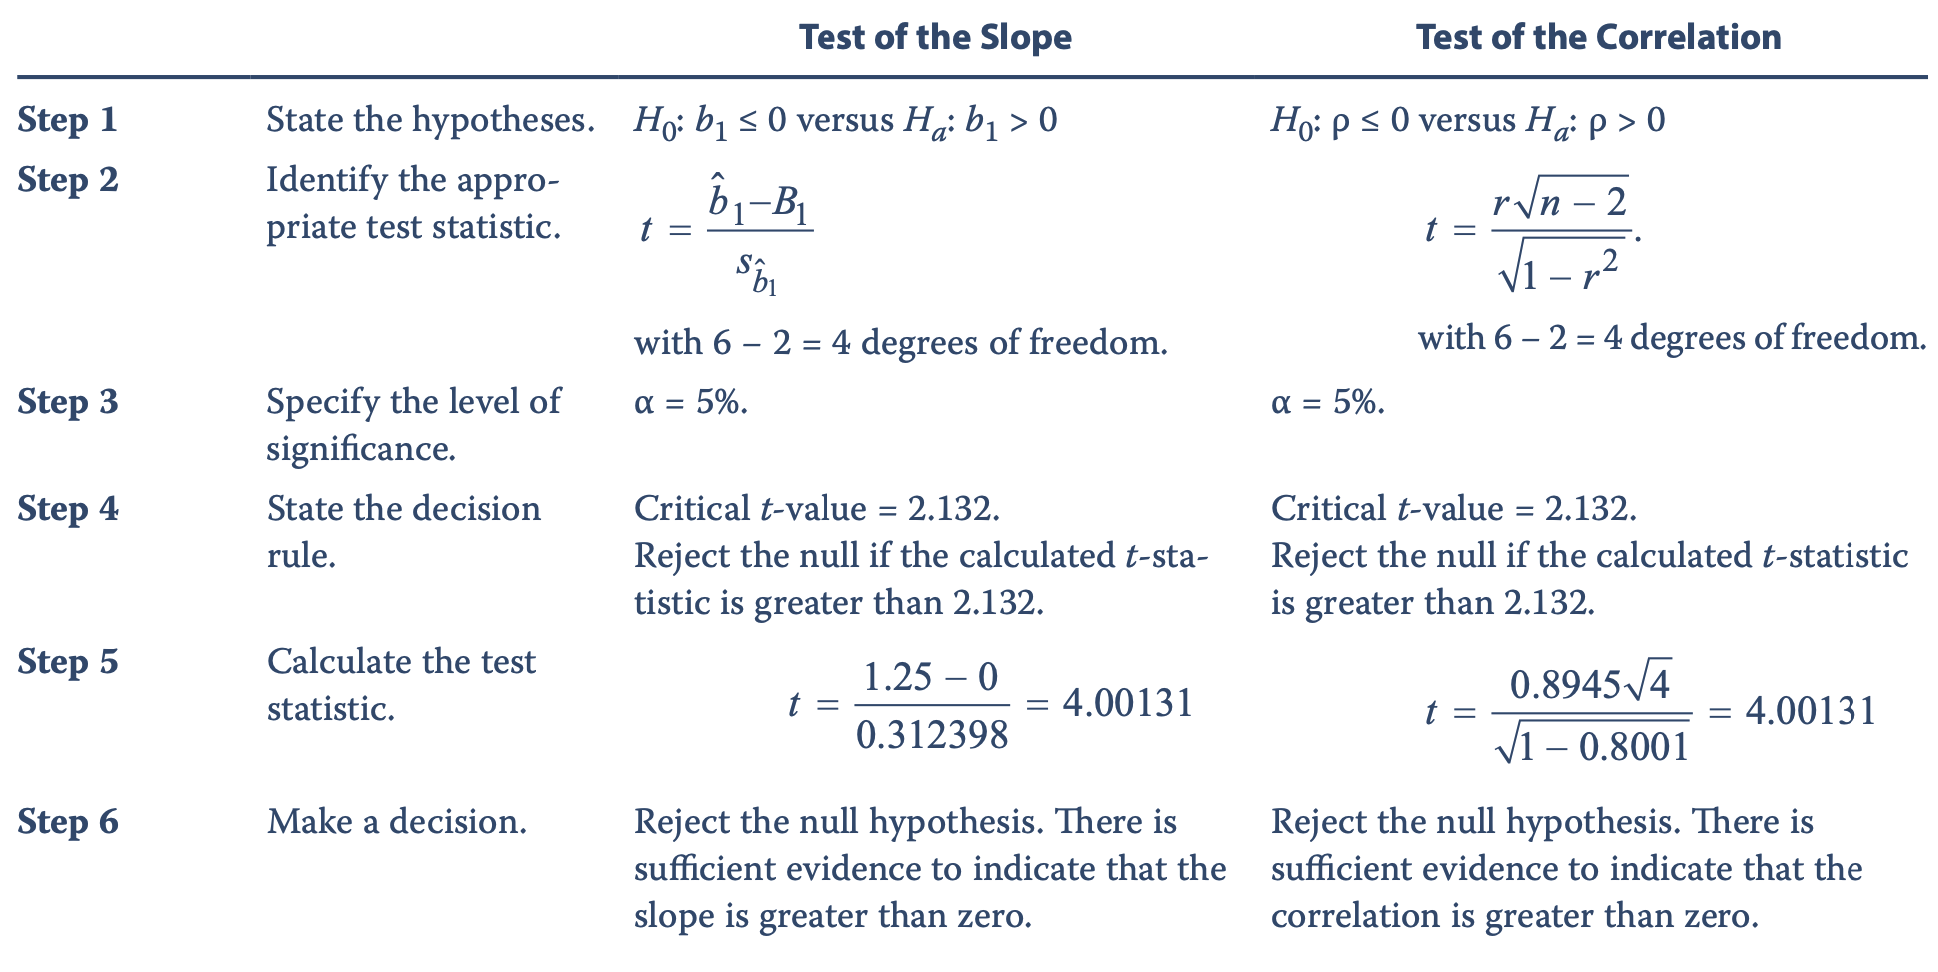
\includegraphics[scale=0.5]{quant/onesidetest}
\caption{One-sided tests for slop and correlation, single regression}
\end{figure}

\begin{definition} The \hlt{predicted values confidence interval} is defined as $\hat{Y} \pm (t_{\alpha/2} \times SE_{f})$, where $t_{\alpha/2}$ is the critical two-tailed t-value for the confidence level $\alpha$, with degrees of freedom $df = n-2$, and $SE_f$ is the standard error of the forecast. 
 Note that $SE_f^2 = SEE^2 \left[1 + \frac{1}{n} + \frac{(X - \overline{X})^2}{(n-1)\sigma^2_X} \right]$, where $\sigma^2_X$ is the variance of the independent variable, $X$ is the value of the independent variable for which the forecast was made.
\end{definition}

\begin{figure}[H]
\centering
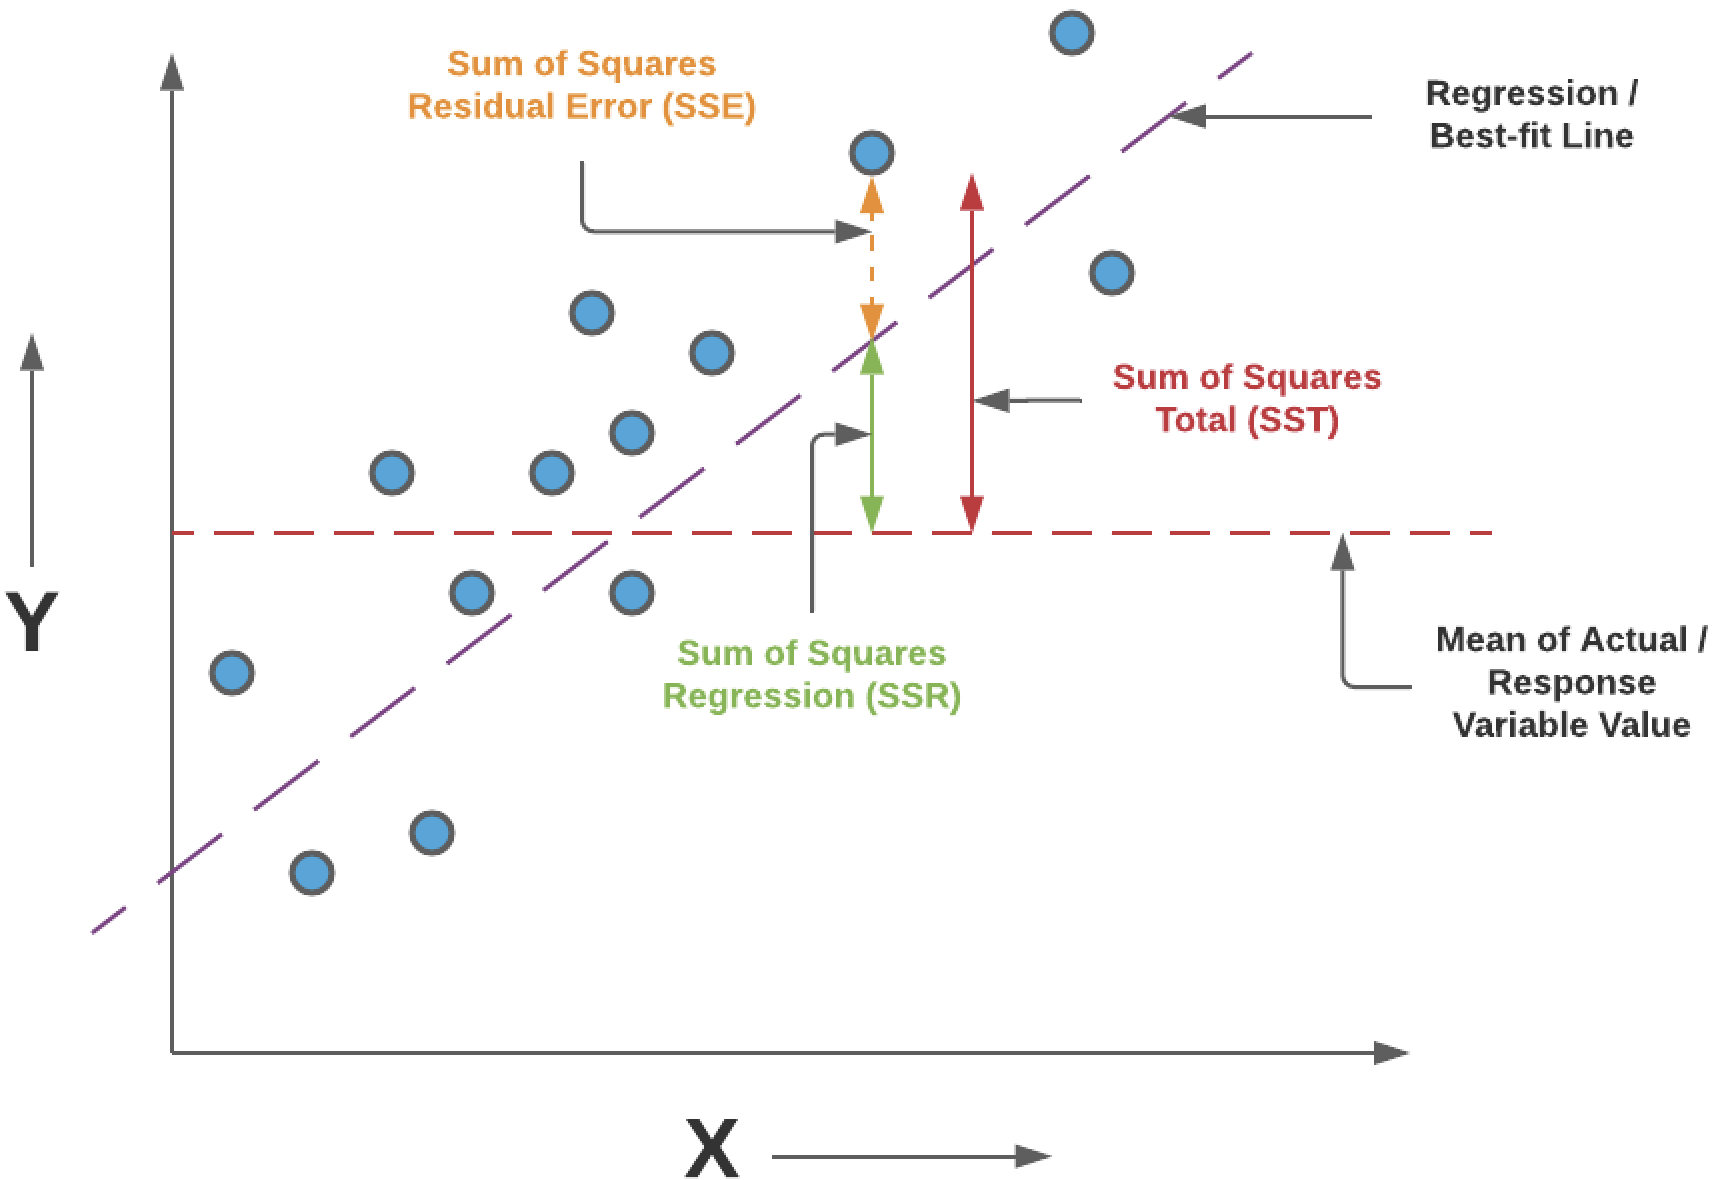
\includegraphics[scale=0.25]{quant/ssr}
\caption{Regression Error Terms}
\end{figure}
 
\begin{definition} \hlt{Analysis of Variance (ANOVA)} analyses the total variability of the dependent variable:
\begin{enumerate}[label=\roman*.]
\setlength{\itemsep}{0pt}
\item Sum of total squares (SST): measures total variation in dependent variable. Sum of squared differences between actual and mean value, $SST = \sum\limits_{i=1}^n (Y_i - \overline{Y})^2$.
\item Sum of squares regression (SSR): measures variation in dependent variable as explained by independent variable. Sum of square distances between predicted and mean value, $SSR = \sum\limits_{i=1}^n (\hat{Y}_i - \overline{Y})^2$.
\item Sum of squares residual error (SSE): measures unexplained variation in dependent variable. Sum of squared vertical distance between actual and predicted values. $SSE = \sum\limits_{i=1}^n (Y_i - \hat{Y})^2$.
\item Mean squares regression (MSR): $MSR = \frac{SSR}{k}$, where $k$ is number of independent variables.
\item Mean squares error (MSE): $MSE = \frac{SSE}{n-k-1}$, where $k$ is number of independent variables.
\item Standard error of estimate (SEE): $SEE = \sqrt{\frac{\sum\limits_{i=1}^n (Y_i - \hat{Y})}{n-2}} = \sqrt{MSE}$.
\item Standard error of intercept: $SE_{\hat{b}_0} = \sqrt{\frac{1}{n} + \frac{\overline{X}^2}{\sum\limits_{i=1}^n(X_i - \overline{X})^2}}$
\end{enumerate}
\end{definition}

\begin{definition} \hlt{Test of Slope Intercept Significance}\\
Two-tailed test $H_0: b_0 \leq B_0$ against $H_{\alpha} : b_0 > B_0$.\\
Test statistic is $t = \frac{\hat{b}_0 - B_0}{SE_{\hat{b}_0}}$, with degrees of freedom $df = n-2$.\\
Reject $H_0$ if $t > t_{\alpha}$.
\end{definition}

\begin{figure}[H]
\centering
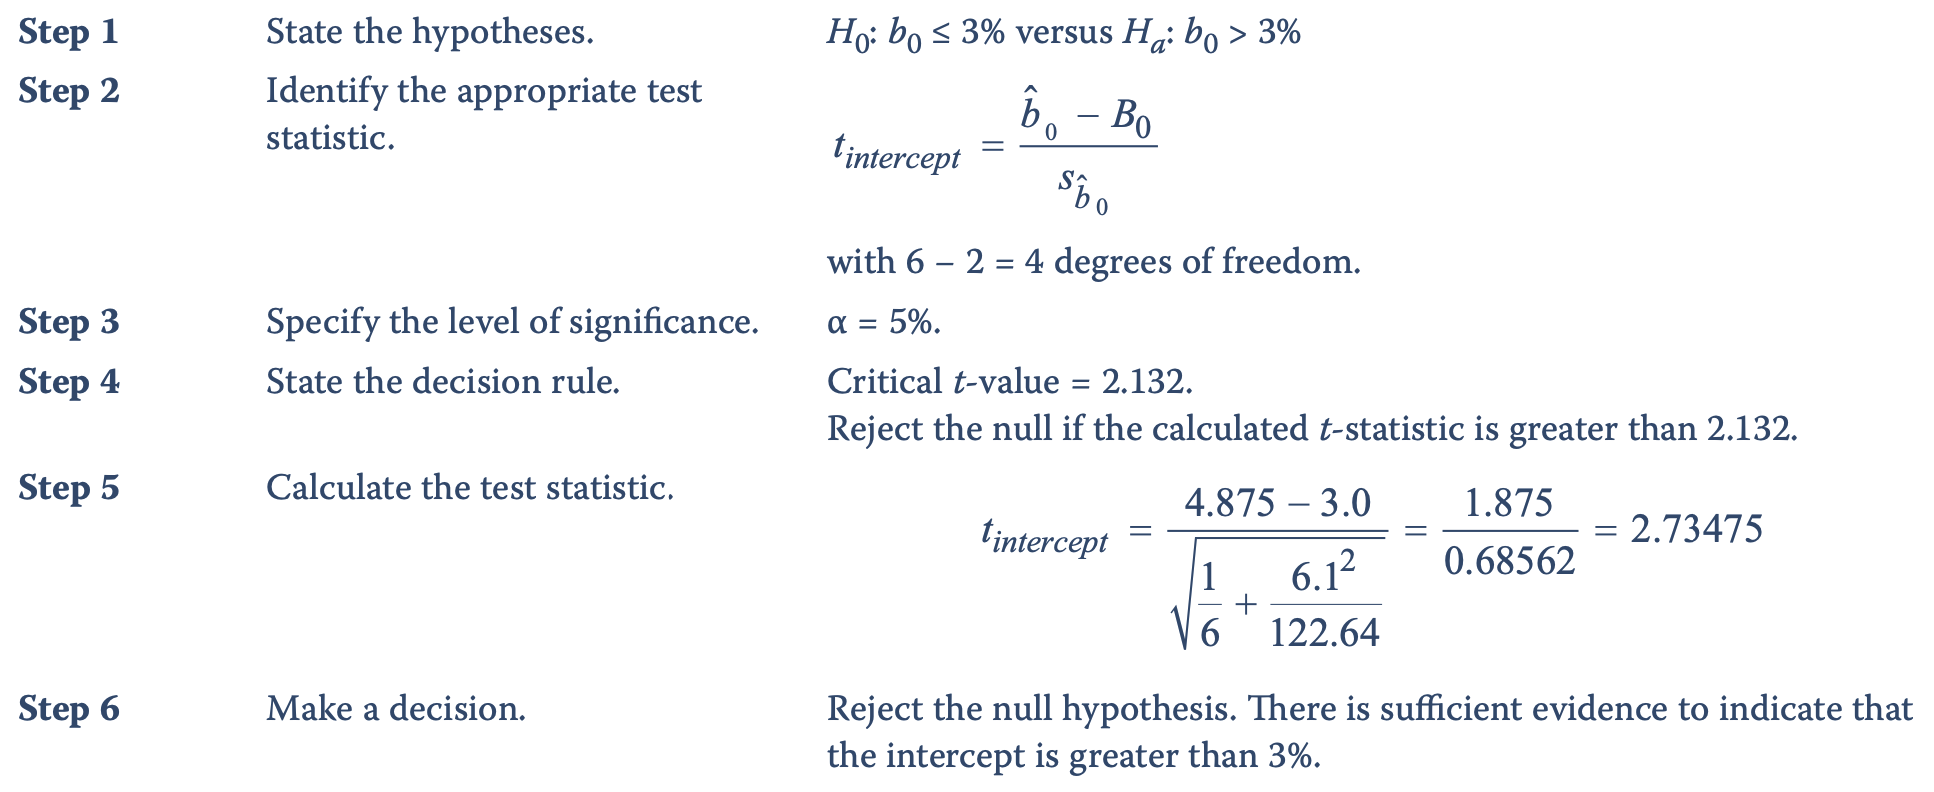
\includegraphics[scale=0.5]{quant/slopeintercept}
\caption{Slope intercept test of regression}
\end{figure}

\begin{definition} \hlt{Coefficient of determination, $R^2$}, measure goodness of fit of regression to data.
\begin{equation}
R^2 = \frac{SST - SSE}{SST} = \frac{SSR}{SST} \nonumber
\end{equation}
\end{definition}

Note that $R^2$ do not allow us to know if coefficients are statistically significant. There is no info on bias in estimated coefficients and predicted values. There is no info if model fit is good as well.

\begin{definition} \hlt{Adjusted $R^2$}, adjusts for degrees of freedom.
\begin{equation}
\overline{R}^2 = 1 - \left[\left(\frac{n-1}{n-k-1} (1-R^2) \right) \right] \nonumber
\end{equation}
where $k$ is number of independent variables.
\end{definition}

If we are adding new independent variable to the regression, if the coefficient t-statistics $> \abs{1.0}$, then $\overline{R}^2$ will increase. If coefficient t-statistics $< \abs{1.0}$, then $\overline{R}^2$ will decrease.

\begin{definition} \hlt{Information Criterions}
\begin{enumerate}[label=\roman*.]
\setlength{\itemsep}{0pt}
\item \hlt{Akaike Information Criterion (AIC)}: evaluate model parsimony. Lower AIC means better fitting.
\begin{equation}
AIC = n \ln(\frac{SSE}{n}) + 2(k+1) \nonumber
\end{equation}
where $n$ is the sample size, k is number of independent variables.
\item \hlt{Bayesian Information Criterion (BIC)}: gives greater penalty than AIC if model has more parameters. Lower BIC means better fitting.
\begin{equation}
BIC = n \ln(\frac{SSE}{n}) + \ln(n)(k+1) \nonumber
\end{equation}
\end{enumerate}
\end{definition}

AIC is preferred if model is used for prediction. BIC is preferred if best goodness of fit is desired.


\newpage

\subsection{Time Series Analysis}

\subsubsection{Trend Model}

\begin{definition} \hlt{Linear Trend Model}\\
Dependent variable changes at a constant rate with them.
\begin{equation}
y_t = b_0 + b_1 t + \epsilon_t, \ \ \ t \in {1, \ldots, T} \nonumber
\end{equation}
Ordinary Least Squares (OLS) is used to estimate coefficient, to get $\hat{Y}_t = \hat{B}_0 + \hat{B}_1 (t)$\\
Trend models may use Durbin-Watson test for serial correlation.
\end{definition}

\begin{definition} \hlt{Log-Linear Trend Models}\\
Used in cases where there is exponential growth.
\begin{equation}
\ln (y_t) = b_0 + b_1 t + \epsilon_t, \ \ \ t \in {1, \ldots, T} \nonumber
\end{equation}
\end{definition}

\begin{figure}[H]
\centering
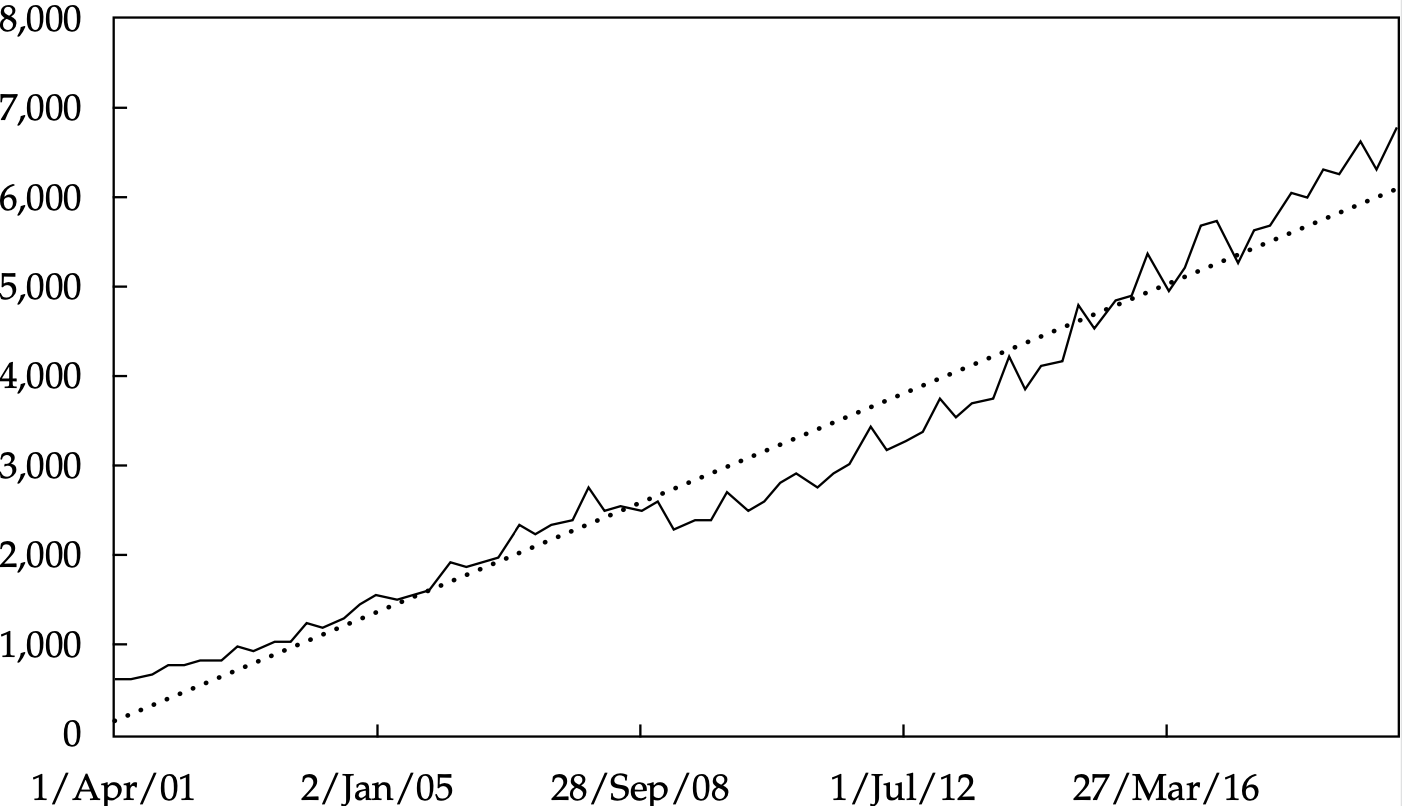
\includegraphics[scale=0.27]{/quant/lintrend}
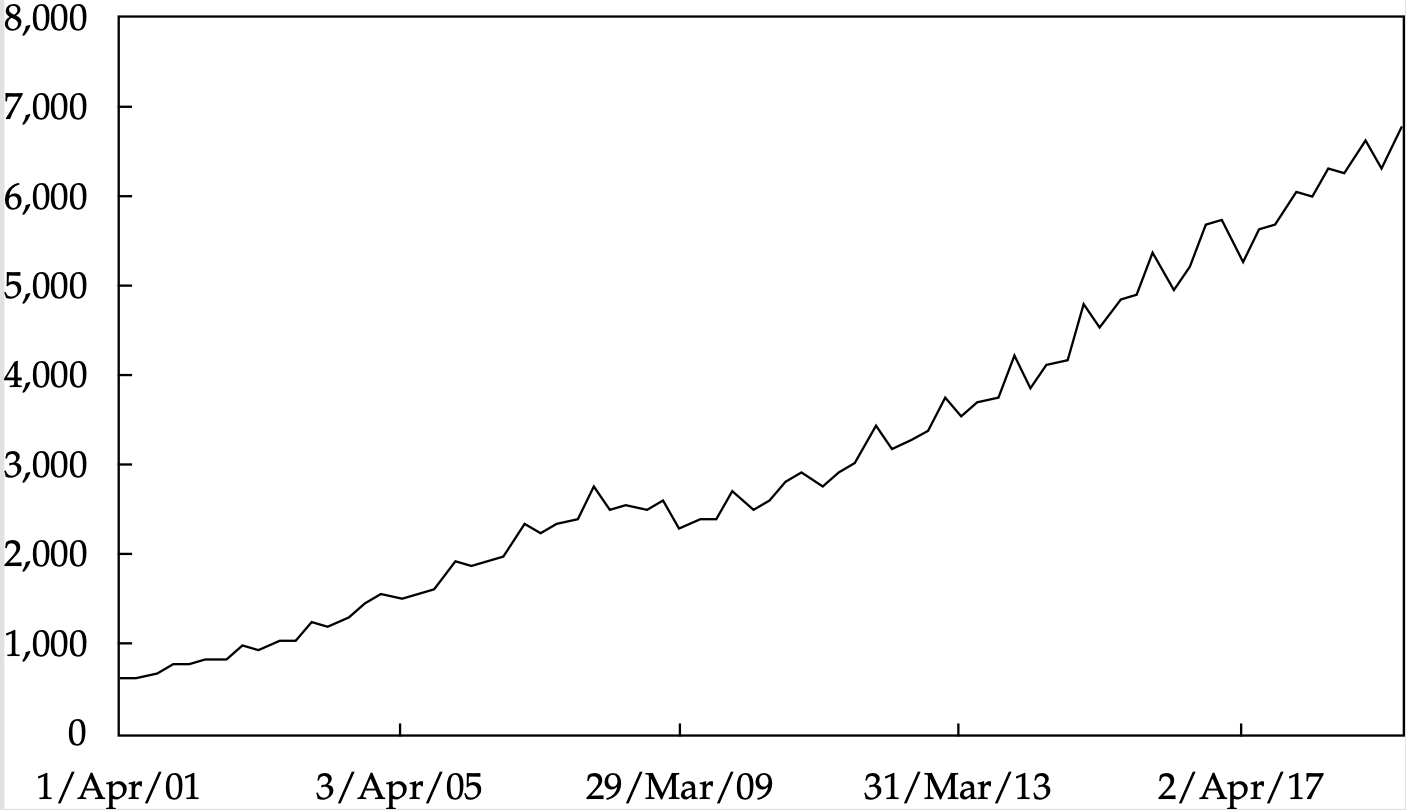
\includegraphics[scale=0.27]{/quant/exptrend}
\caption{Linear trend, exponential trend}
\end{figure}

\subsubsection{AR Models}

\begin{definition} \hlt{Autoregressive (AR) Model of Order $p$}\\
Dependent variable is regressed against one or more lagged values of itself. For a model of order $p$, AR($p$),
\begin{equation}
x_t = b_0 + \sum\limits_{i=1}^p b_i x_{t-p} + \epsilon_t \nonumber
\end{equation}
\end{definition}

\begin{definition} \hlt{Covariance Stationary}\\
Statistical inference based on OLS estimates for AR($p$) model is invalid unless time series is covariance stationary:
\begin{enumerate}[label=\roman*.]
\setlength{\itemsep}{0pt}
\item Constant and finite expected value (expected value is constant over time; mean-reverting)
\item Constant and finite variance (volatility around its mean does not change over time)
\item Constant and finite covariance between values at any given lag
\end{enumerate}
\end{definition}

\begin{remark} \hlt{Test of Autocorrelation}
\begin{enumerate}[label=\roman*.]
\setlength{\itemsep}{0pt}
\item Compute the AR($p$) model using linear regression
\item Calculate the autocorrelation of the model residuals.\\
Note, the $k$-th order estimated autocorrelation $\hat{\rho}_k$ and autocorrelations of error term $\rho_{\epsilon, k}$ are as follows
\begin{align}
\hat{\rho}_k = \frac{\sum\limits_{t=k+1}^T [(x_t - \overline{x}) (x_{t-k} - \overline{x})]}{\sum\limits_{t=1}^T (x_t - \overline{x})^2}, \ \ \ \ \rho_{\epsilon, k} = \frac{E(\epsilon_t \epsilon_{t-k})}{\sigma_{\epsilon}^2} \nonumber
\end{align}
\item Test if the residual correlations are significantly from zero.\\
If model is correctly specified, none of the autocorrelations will be statistically significant.\\
To test for significant,$H_0: \rho_{\epsilon, k} = 0$ and $H_a: \rho_{\epsilon, k} \neq 0$.  $t$-statistic with $df = T-2$ is
\begin{equation}
t = \frac{\rho_{\epsilon, k}}{1/\sqrt{T}} \nonumber
\end{equation}
Note the standard error of residual correlation is $1/\sqrt{T}$.
\end{enumerate}
\end{remark}

\begin{remark} \hlt{Mean Reversion}\\
Time series exhibits tendency to move towards its mean.\\
For AR($1$), mean reverting is when $x_t = b_0 + b_1 x_t$, hence mean reverting level is $x_t = \frac{b_0}{1-b_1}$.\\
All covariance stationary time series have a finite mean-reverting level.
\end{remark}

\begin{remark} \hlt{Types of Forecasts}
\begin{enumerate}[label=\roman*.]
\setlength{\itemsep}{0pt}
\item In-Sample Forecasts: $\hat{Y}$ made within the range of data used to estimate the model.
\item Out-of-Sample Forecasts: made outside of the sample period, provides test of whether model has predictive power in real world.
\end{enumerate}
\end{remark}

\begin{remark} \hlt{Root Mean Squared Error (RMSE)}\\
RMSE is used to compare accuracy of AR($p$) models for out-of-sample values.
\begin{equation}
RMSE = \sqrt{\sum\limits_{i=1}^n \frac{(\hat{Y}_i - Y_i)^2}{n}} \nonumber
\end{equation}
where $\hat{Y}_i$ are predicted values, $Y_i$ are actual values, $n$ is number of observations.\\
Model with lowest RMSE for in-sample data may not be model with lowest RMSE for out-of-sample data.\\
Model with lower RMSE for out-of-sample data will have lower forecast error and better predictive power.
\end{remark}

\begin{definition} \hlt{Random Walk}\\
Time series in which the value of the series in one period is the value of the series in the previous period plus an unpredictable random error.
\begin{align}
x_t &= x_{t-1} + \epsilon_t \nonumber \\
E[\epsilon_t] &= 0, E[\epsilon_t^2] = \sigma^2 \nonumber \\
\text{Cov}[\epsilon_t, \epsilon_s] &= E[\epsilon_t \epsilon_s] = 0 \ \ \text{if} \ \ i \neq j \nonumber
\end{align}
Expected value of error is zero, variance of error is constant, there is no serial correlation in error.
\end{definition}

\begin{definition} \hlt{Random Walk with Drift}\\
Time series expected to increase or decrease by a constant amount each period.
\begin{equation}
x_t = b_0 + b_1 x_{t-1} + \epsilon_t \nonumber
\end{equation}
\end{definition}

\begin{remark} \hlt{Properties of Random Walk}\\
Random walk has an undefined mean-reverting level ($\frac{b_0}{1-b_1} = \frac{b_0}{0}$), hence is not covariance stationary.\\
All random walks have a unit root $b_1 = 1$, hence least squares regression cannot be used.
\end{remark}

\begin{definition} \hlt{First Difference}\\
Subtracts value of the time series in the first prior period from the current value of the time series.
\begin{equation}
\Delta x_t = x_t - x_{t-1} \nonumber
\end{equation}
\end{definition}

\begin{remark} \hlt{Dickey-Fuller Unit Root Test}\\
Given an AR($1$) model $x_t = b_1 x_{t-1} + \epsilon_t$, take the first difference to get $\Delta x_t = (b_1 - 1)x_{t-1} + \epsilon_t$.\\
Let $g_1 = b_1 -1 $. If there is a unit root in the model, then $g_1 = 0$.\\
Hypothesis test is then $H_0: g_1 = 0$ (has unit root, non-stationary), and $H_a: g_1 < 0$ (no unit root, stationary)\\
$t$-statistic is computed in a conventional manner for $\hat{g}_1$, but a revised set of values are used for the test.
\end{remark}

\begin{remark} \hlt{Seasonality}\\
Pattern that tends to repeat form year to year.\\
To adjust for seasonality in an AR($p$) model, add additional lag, i.e., $x_t = b_0 + b_1 x_{t-1} + b_2 x_{t-4} + \epsilon_t$
\end{remark}

\subsubsection{ARMA, ARCH Models}

\begin{definition} \hlt{Moving Average (MA) Models}\\
The MA($q$) model is as follows:
\begin{align}
x_t = \mu + \sum\limits_{i=1}^q \theta_i \epsilon_{t-i} + \epsilon_t, \ \ \ E[\epsilon_t] = 0, E[\epsilon_t^2] = \sigma^2, \text{Cov}[\epsilon_t, \epsilon_s] = E[\epsilon_t \epsilon_s] = 0 \ \ \text{for} \ \ t \neq s \nonumber
\end{align}
where $\mu$ is mean of the series, $\theta$ are coefficients of the series
\end{definition}

\begin{definition} \hlt{Autoregressive Moving Average (ARMA) Model}\\
Combines both autoregressive lags of dependent variable and moving-average errors. ARMA($p,q$) is as follows:
\begin{equation}
x_t = b_0 + \sum\limits_{i=1}^p b_i x_{t-i} + \mu + \sum\limits_{i=1}^q \theta_i \epsilon_{t-i} + \epsilon_t, \ \ \ E[\epsilon_t] = 0, E[\epsilon_t^2] = \sigma^2, \text{Cov}[\epsilon_t, \epsilon_s] = E[\epsilon_t \epsilon_s] = 0 \ \ \text{for} \ \ t \neq s \nonumber
\end{equation}
Note that parameters in ARMA models can be very unstable to slight perturbations.\\
Choosing the right $p,q$ values is more of an art than a science, as criteria for choosing is far from perfect.\\
Even after a model is selected, the model may not forecast well.
\end{definition}

\begin{definition} \hlt{Autoregressive Conditional Heteroskedasticity (ARCH) Model}\\
Used to test for autoregressive conditional heteroskedasticity. The time series variance of residuals in on e period is dependent on variance of residuals in preceding periods. An ARCH($q$) mode is as follows
\begin{equation}
\epsilon_t \sim N \left( 0, a_0 + \sum\limits_{i=1}^q a_i \epsilon_{t-1}^2 \right), \ \ \ \epsilon_t^2 = a_0 + \sum\limits_{i=1}^q a_i \epsilon_{t-1}^2 \nonumber
\end{equation}
Using $t$-statistics, if $a_i$ is statistically significant from zero, then series is ARCH($q$).
\end{definition}

\subsubsection{Regression on Multiple Timeseries}

\begin{remark} \hlt{Multiple Timeseries Regression}\\
To regress a time series $y_t$ on another time series $x_t$, i.e., $y_t = b_0 + b_1 x_t + \epsilon_t$.\\
As there are two different time series $x_t$ and $y_t$, either of both can be subject to non-stationarity.\\
First estimate the regression $y_t = b_0 + b_1 x_t + \epsilon_t$, then to run separate Dickey-Fuller tests with possible results:
\begin{enumerate}[label=\roman*.]
\setlength{\itemsep}{0pt}
\item Neither have unit root, i.e., both time series are covariance stationary.
\item Only dependent variable time series is covariance stationary, i.e, $H_0$ for dependent variable not rejected.
\item Only independent variable time series is covariance stationary, i.e, $H_0$ for independent variable not rejected.
\item Neither is covariance stationary, and both time series are not co-integrated.
\item Neither is covariance stationary, and both time series are co-integrated.
\end{enumerate}
For scenario $1$, linear regression may be used, and coefficients should be statistically reliable.\\
For scenario $2, 3$, linear regression may not be used, as coefficients will not be statistically reliable.\\
For scenario $4, 5$, whether linear regression can be used depends on whether two time series are co-integrated.
\end{remark}

\begin{definition} \hlt{Co-Integration of Time Series}\\
Two time series are economically linked, or follow the same trend, and relationship is not expected to change.\\
If two time series are co-integrated, the error term from regressing on eon the other is covariance stationary.
\begin{enumerate}[label=\roman*.]
\setlength{\itemsep}{0pt}
\item Estimate regression $y_t = b_0 + b_1 x_t + \epsilon_t$.
\item Test if $\epsilon_t$ has unit root with Dickey-Fuller, but use critical values by Engle and Granger (DF-EG test).
\item If test rejects $H_0$, then $\epsilon_t$ is covariance stationary, and both are co-integrated.
\end{enumerate}
\end{definition}

\begin{definition} \hlt{Steps for Time-Series Forecasting}
\begin{enumerate}[label=\roman*.]
\setlength{\itemsep}{0pt}
\item Understand investment problem, casual relationships of variables
\item Plot time series for indications of seasonality, structural shifts, linear or exponential trend.
\item If no seasonality or structural shifts, use a trend model.
\begin{enumerate}[label=\arabic*.]
\setlength{\itemsep}{0pt}
\item If data plot is a straight line, use a linear trend model
\item If data plot is a curve, use a log-linear trend model
\end{enumerate}
\item Run trend analysis, compute the residuals, test for serial correlation using Durbin-Watson test
\begin{enumerate}[label=\arabic*.]
\setlength{\itemsep}{0pt}
\item If no serial correlation, the trend model can be used.
\item If serial correlation is detected, use a more complex model
\end{enumerate}
\item If data has serial correlation, reexamine the data for stationarity before running AR model. If it is not stationary, treat the data for use in an AR model as follows:
\begin{enumerate}[label=\arabic*.]
\setlength{\itemsep}{0pt}
\item If data has linear trend, first-difference the data
\item If data has exponential trend, first-difference the natural log of the data
\item If there is structural shift in the data, run two separate models
\item If data has seasonal component, incorporate seasonality into the AR model
\end{enumerate}
\item After first-differencing, if series is covariance stationary, run AR($1$), test for serial correlation \& seasonality.
\begin{enumerate}[label=\arabic*.]
\setlength{\itemsep}{0pt}
\item If there is no remaining serial correlation, model may be used
\item If serial correlation is detected, incorporate lagged values of the variable (possibly including one for seasonality) into the AR model until serial correlation has been removed.
\end{enumerate}
\item Test residuals with ARCH. Regress square residuals on squared lagged value of residuals and test if resulting coefficient is significantly different from zero.
\begin{enumerate}[label=\arabic*.]
\setlength{\itemsep}{0pt}
\item If coefficient is not significantly different from zero, model may be used.
\item If coefficient is significantly different from zero, ARCH is present. Use generalised least squares.
\end{enumerate}
\item Perform tests of model’s out-of-sample forecasting performance with RMSE.
\end{enumerate}
\end{definition}


\newpage

\subsection{Machine Learning}

\begin{flushleft}
ML Algorithm Overview
\begin{tabularx}{\textwidth}{p{6.5em}|p{7.7em}|p{9.5em}|X}
\hline
\rowcolor{gray!30}
Variable Input & ML Classification & ML Type & ML Algorithms \\
\hline
Continuous & Supervised & Regression &
\xxx Linear, penalised regression/LASSO
\xxx Logistic
\xxx Classification and Regression Tree (CART)
\xxx Random Forest \\
& Unsupervised & Dimension Reduction & 
\xxx Principal Component Analysis (PCA) \\
& & Clustering &
\xxx K-Means
\xxx Hierarchical \\
\hline
Categorical & Supervised & Classification &
\xxx Logistic
\xxx Support Vector Machine (SVM)
\xxx K-Nearest Neighbour (KNN)
\xxx Classification and Regression Tree (CART) \\
& Unsupervised & Dimension Reduction & 
\xxx Principal Component Analysis (PCA) \\
& & Clustering &
\xxx K-Means
\xxx Hierarchical \\
\hline
Both & Both & &
\xxx Neural Networks
\xxx Deep Learning
\xxx Reinforcement Learning \\
\hline
\end{tabularx}
\end{flushleft}

\begin{remark} \hlt{Sources of Out-of-Sample Error}
\begin{enumerate}[label=\roman*.]
\setlength{\itemsep}{0pt}
\item Bias error: degree to which a model fits the training data. Poor algorithm assumptions lead to high bias, poor approximation, under-fitting, high in-sample error.
\item Variance error: how much the model’s results change in response to new data from validation and test samples. Unstable models pick up noise, produce high variance, overfitting, high out-sample error.
\item Base error: due to randomness of the data
\end{enumerate}
\end{remark}

\begin{figure}[H]
\centering
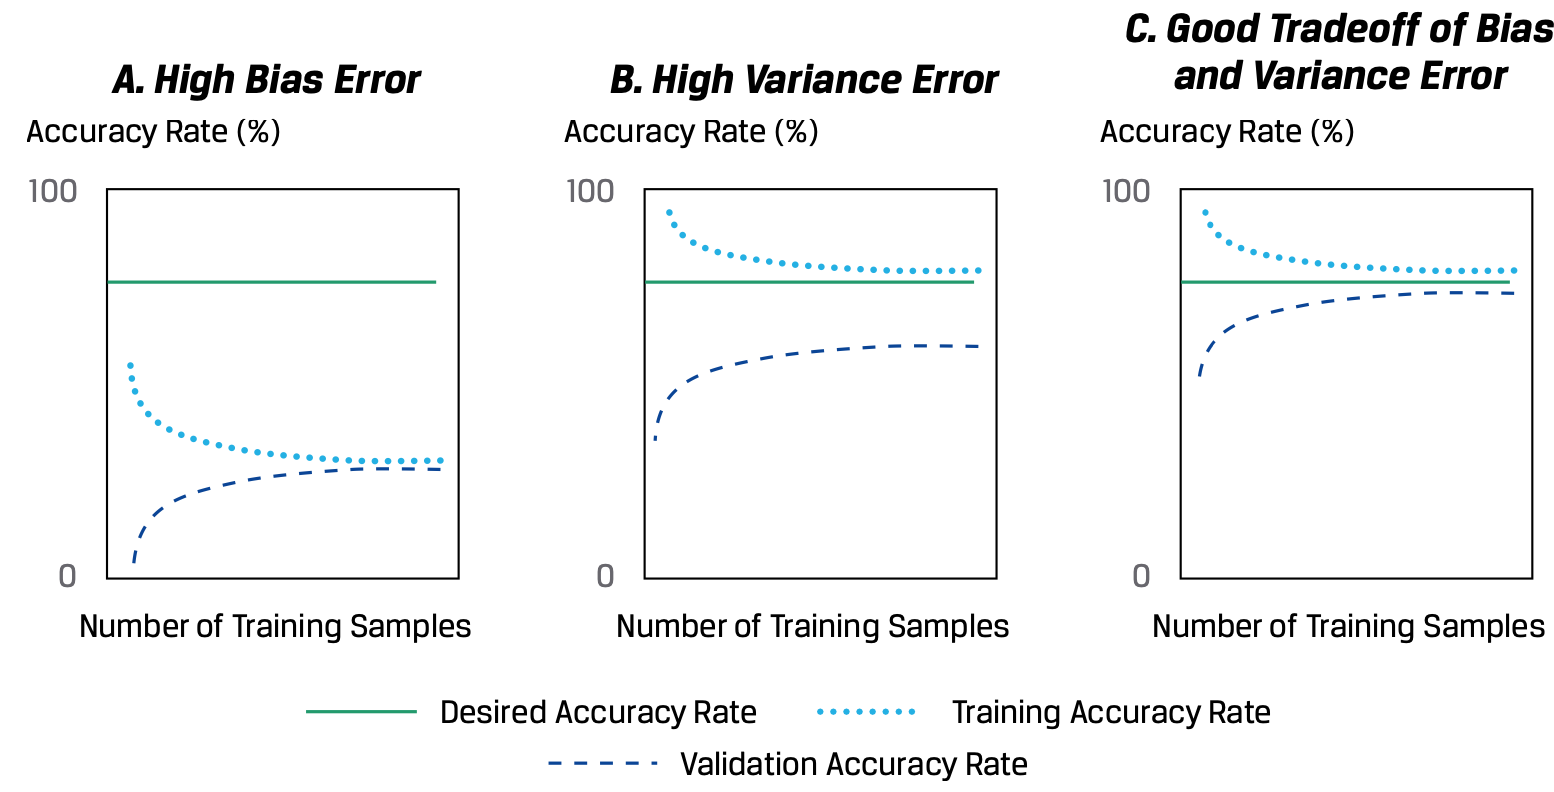
\includegraphics[scale=0.4]{/quant/learningcurves}
\caption{Learning curves showing accuracy in validation and training samples}
\end{figure}

\begin{figure}[H]
\centering
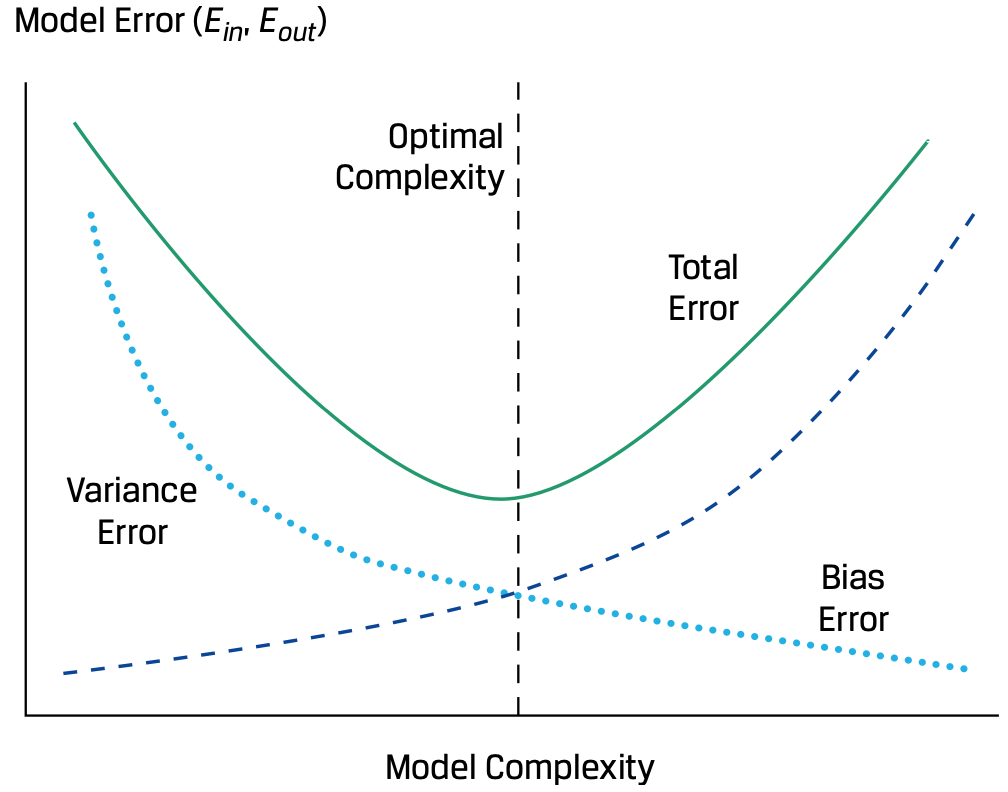
\includegraphics[scale=0.35]{/quant/fittingcurve}
\caption{Fitting curve showing bias-variance tradeoff and model complexity}
\end{figure}

\begin{definition} \hlt{$k$-Fold Cross Validation}\\
Data divided into $k$ samples. Rotate each sample used for validation.\\
Error is then measured for the model in each of the parts, process repeats $k$ times.\\
Average in-sample and out-of-sample error rates are then compiled.
\end{definition}

\begin{definition} \hlt{Penalised Regression}\\
Reduce the problem of overfitting by imposing a penalty based on number of features used.\\
Penalty value increases with number of independent variables used.\\
Penalty exclude features that are not meaningfully contributing to out-of-sample prediction accuracy.\\
Model seek to minimise Sum of Square Errors (SSE) and penalty value. 
\end{definition}

\begin{definition} \hlt{Least Absolute Shrinkage and Selection Operator (LASSO)}\\
In addition to minimising SSE, LASSO minimises the sum of the absolute values of the slope coefficients.\\
LASSO automatically eliminates the least predictive features.
\begin{equation}
\text{Penalty Term} = \lambda \sum\limits_{k=1}^K \abs{\hat{b}_k} \nonumber
\end{equation}
where $\lambda > 0$ is the hyper-parameter that balances between overfitting and parsimonious model.
\end{definition}

\begin{definition} \hlt{Regularisation}\\
Methods that reduce statistical variability in high-dimensional data estimation problems.\\
Aim to reduce regression coefficient estimates toward zero, avoiding complex models and the risk of overfitting
\end{definition}

\begin{definition} \hlt{Support Vector Machine (SVM)}\\
Linear classification algorithm that separates the data into one of two possible classifiers.\\
Algorithm maximises the probability of making a correct prediction by determining the boundary that is farthest away from all the observations, which is a discriminant boundary with margins on the side.\\
Margins are determined by the support vectors, observations that are closest to the boundary.\\
Misclassified observations in training data are handled via soft margin classification. This optimises the tradeoff between a wider margin and classification error.\\
Particularly suited for small to medium-size but complex high-dimensional datasets.
\end{definition}

\begin{figure}[H]
\centering
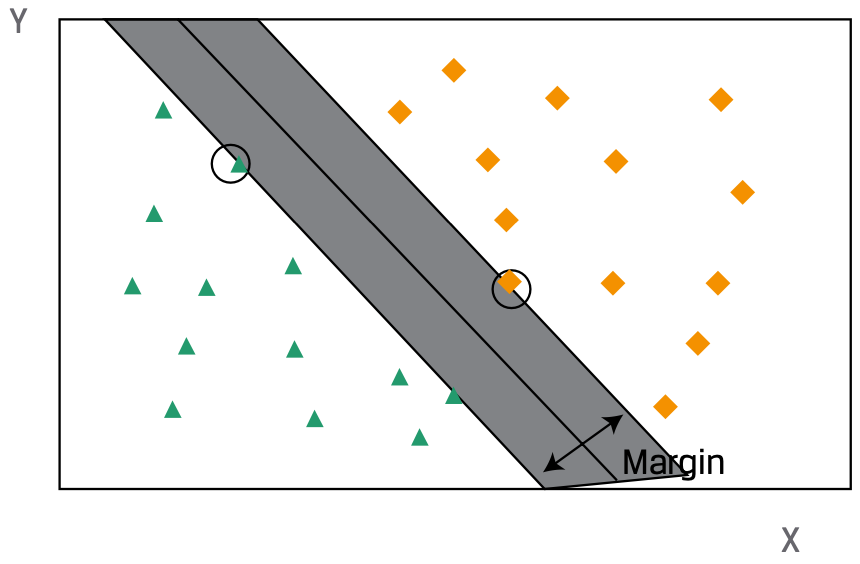
\includegraphics[scale=0.35]{/quant/svm}
\caption{Support Vector Machine}
\end{figure}

\begin{definition} \hlt{$K$-Nearest Neighbour ($K$NN)}\\
Classify an observation based on nearness to the observations in the training sample\\
Hyper-parameter $K$ is specified on number of categories to produce. If $K$ is too small, there is high error rate; if $K$ is too large, result diluted. If $K$ is even, there may be ties, with no clear winner.\\
Requires a distance metric to be specified. Inclusion of irrelevant or correlated features can skew the results.
\end{definition}

\begin{figure}[H]
\centering
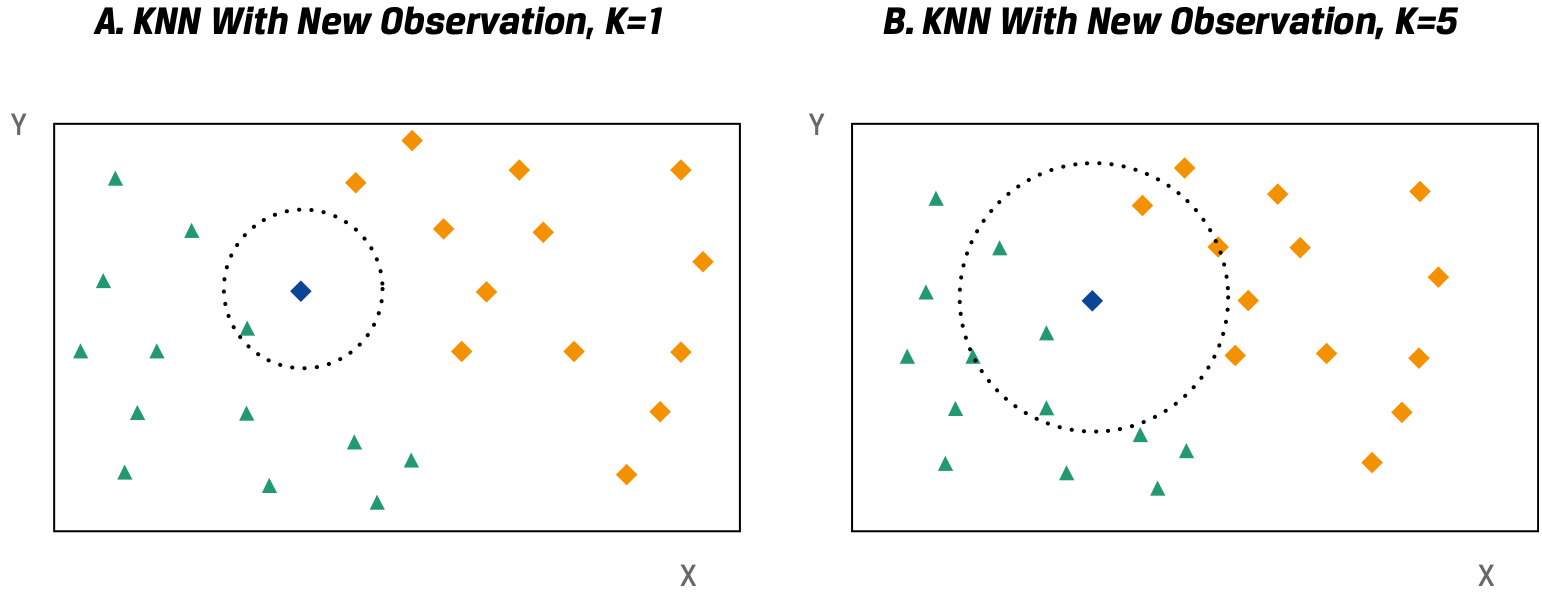
\includegraphics[scale=0.35]{/quant/knn}
\caption{$K$-Nearest Neightbour}
\end{figure}

\begin{definition} \hlt{Classification and Regression Trees (CART)}\\
Appropriate when target variable is categorical, and used when target is binary (classification tree) or a continuous target variable (regression tree).\\
Classification trees assign observations to one of two possible classification at each node. At top of the tree, top feature is selected, and a cutoff value $c$ is estimated.\\
Observations with feature values $> c$ are assigned to one classification, remainder assigned to the other.\\
Tree stops when error cannot be reduced further, resulting in a terminal node.\\
To avoid overfitting, regularisation criteria such as maximum tree depth, maximum number of decision nodes can be specified. Alternatively, sections of tree with minimal explanatory power are pruned.
\end{definition}

\begin{figure}[H]
\centering
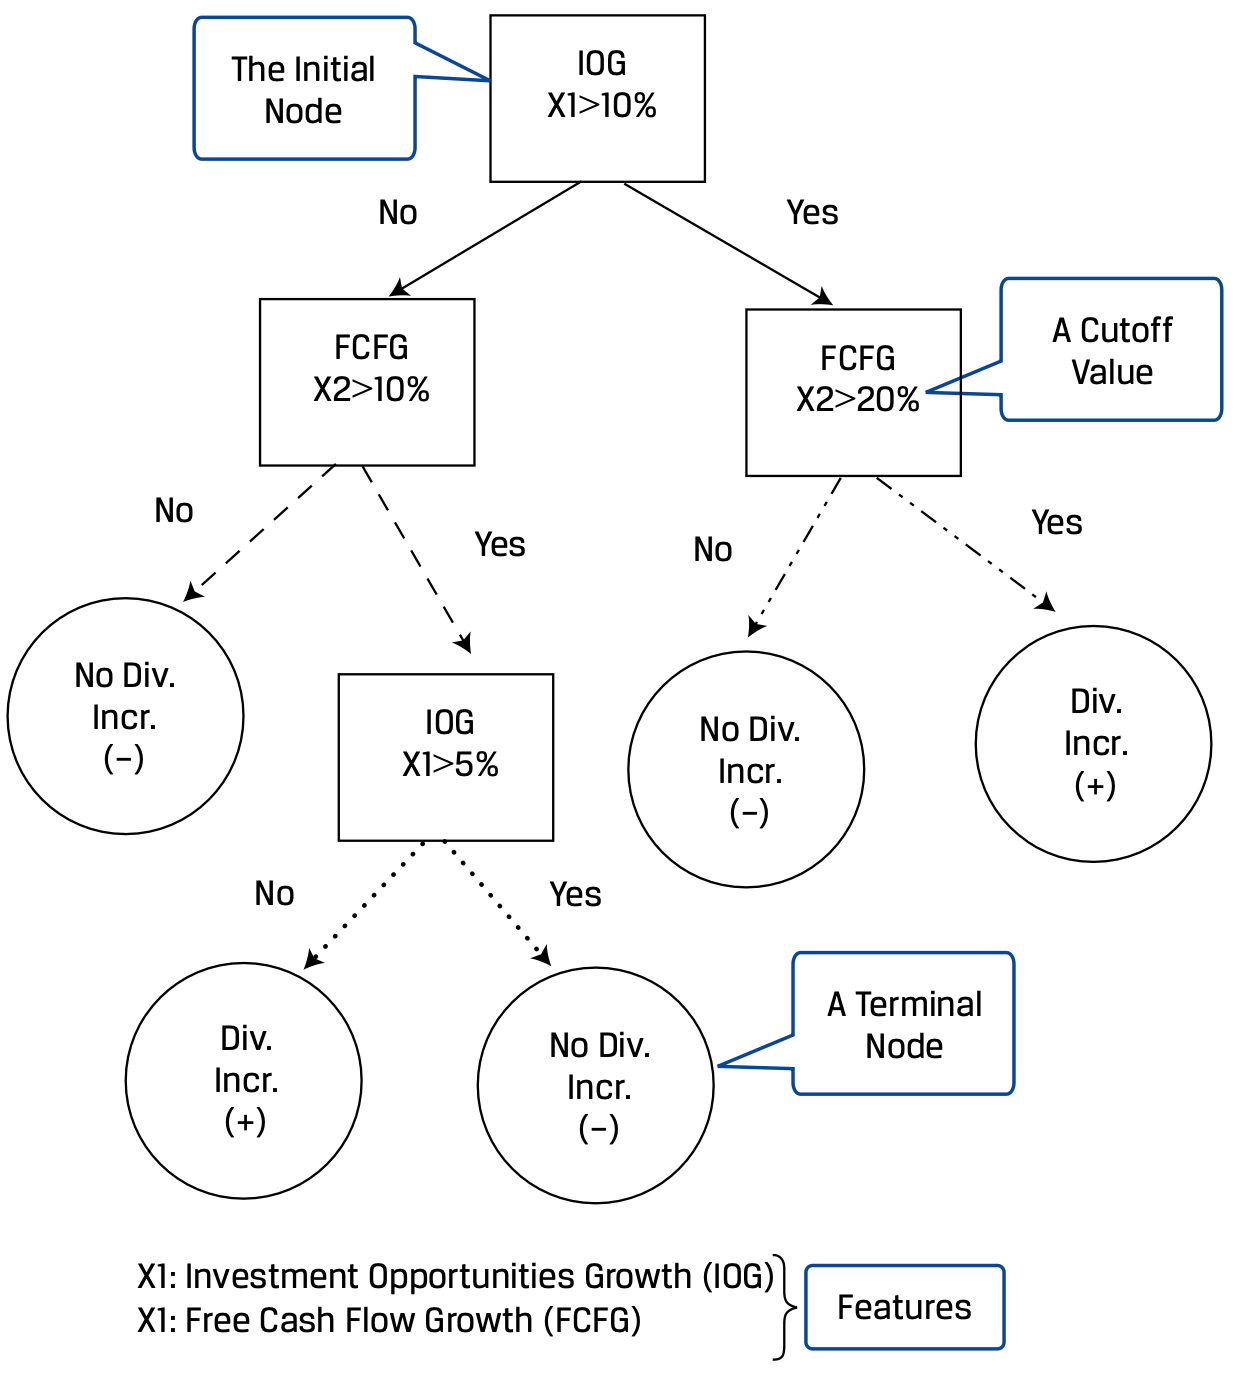
\includegraphics[scale=0.3]{/quant/cart}
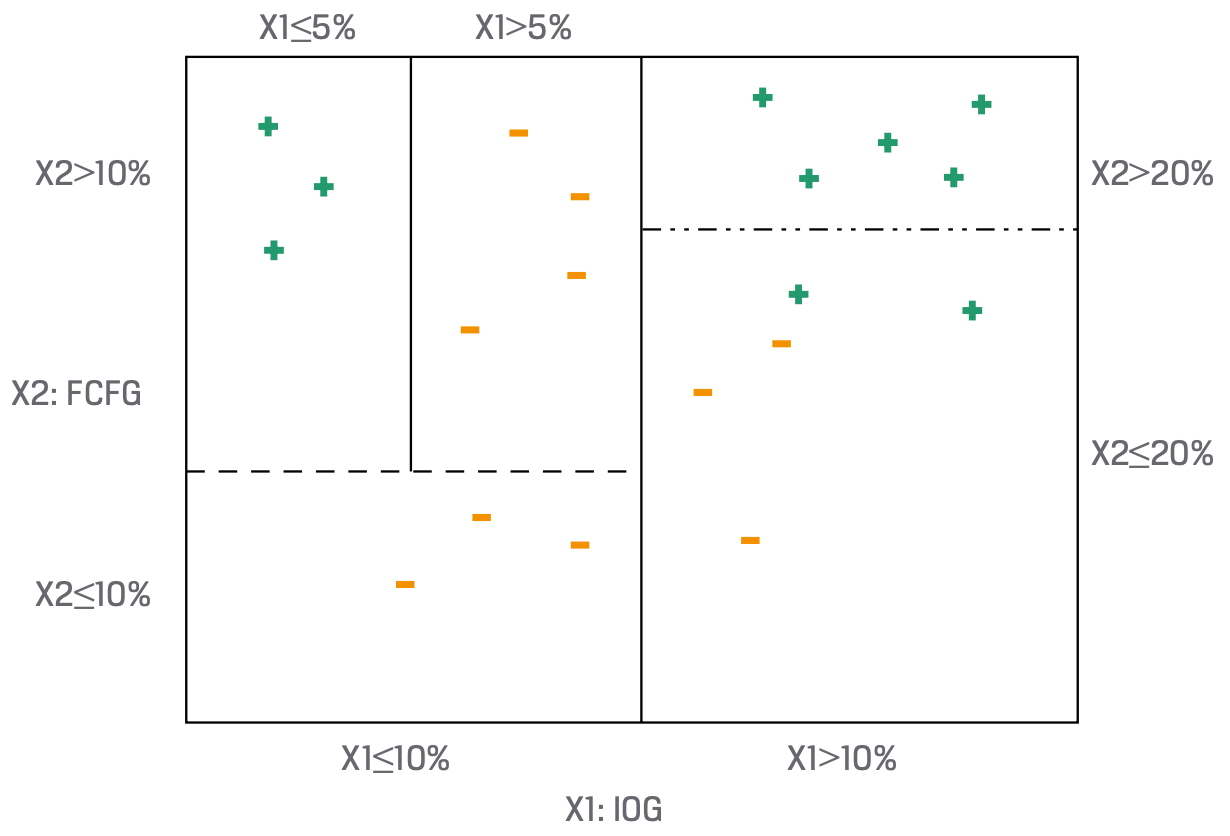
\includegraphics[scale=0.4]{/quant/cartspace}
\caption{CART and the partitioned space}
\end{figure}

\begin{definition} \hlt{Ensemble Learning}\\
Combining the predictions from a collection of models.\\
Produces more accurate and more stable predictions than the best single model. 
\end{definition}

\begin{definition} \hlt{Ensemble Method}\\
Combination of multiple learning algorithms.
\end{definition}

\begin{definition} \hlt{Voting Classifiers}\\
Aggregation of heterogeneous learners, where different algorithms are combined with voting classification.\\
A majority-vote classifier will assign to a new data point the predicted label with the most votes.\\
There is an optimal number of models beyond which performance will deteriorate from overfitting.\\
To look for diversity in the choice of algorithms, modelling techniques, and hypotheses.
\end{definition}

\begin{definition} \hlt{Bootstrap Aggregating (Bagging)}\\
Aggregation of homogeneous learners, where the same algorithm is used on different training data.\\
For each new observation, aggregate the $n$ predictions using a majority-vote classifier for a classification or an average for a regression. Helps to improve the stability of predictions and protects against overfitting the model.
\end{definition}

\begin{definition} \hlt{Random Forest}\\
Collection of a large number of decision trees trained via a bagging method.\\
A randomly selected subset of features is used in creating each tree, which can mitigate the problem of overfitting.\\
Can increase the signal-to-noise ratio because errors across different trees tend to cancel each other out.\\
Note that the transparency of CART is lost when applying random forest classifier.
\end{definition}

\begin{definition} \hlt{Principal Component Analysis (PCA)}\\
Used to summarise or transform highly correlated features of data into a few main, uncorrelated composite variables. Transforms the covariance matrix of features into eigenvectors and eigenvalues.\\
Eigenvectors define new, mutually uncorrelated composite variables that are linear combinations of the original features. Eigenvalue gives proportion of total variance in the initial data that is explained by each eigenvector.
\end{definition}

\begin{definition} \hlt{Scree Plots}\\
Show the proportion of total variance in the data explained by each principal component.\\
The smallest number of principal components that collectively capture $85\%–95\%$ of total variance are retained.
\end{definition}

\begin{figure}[H]
\centering
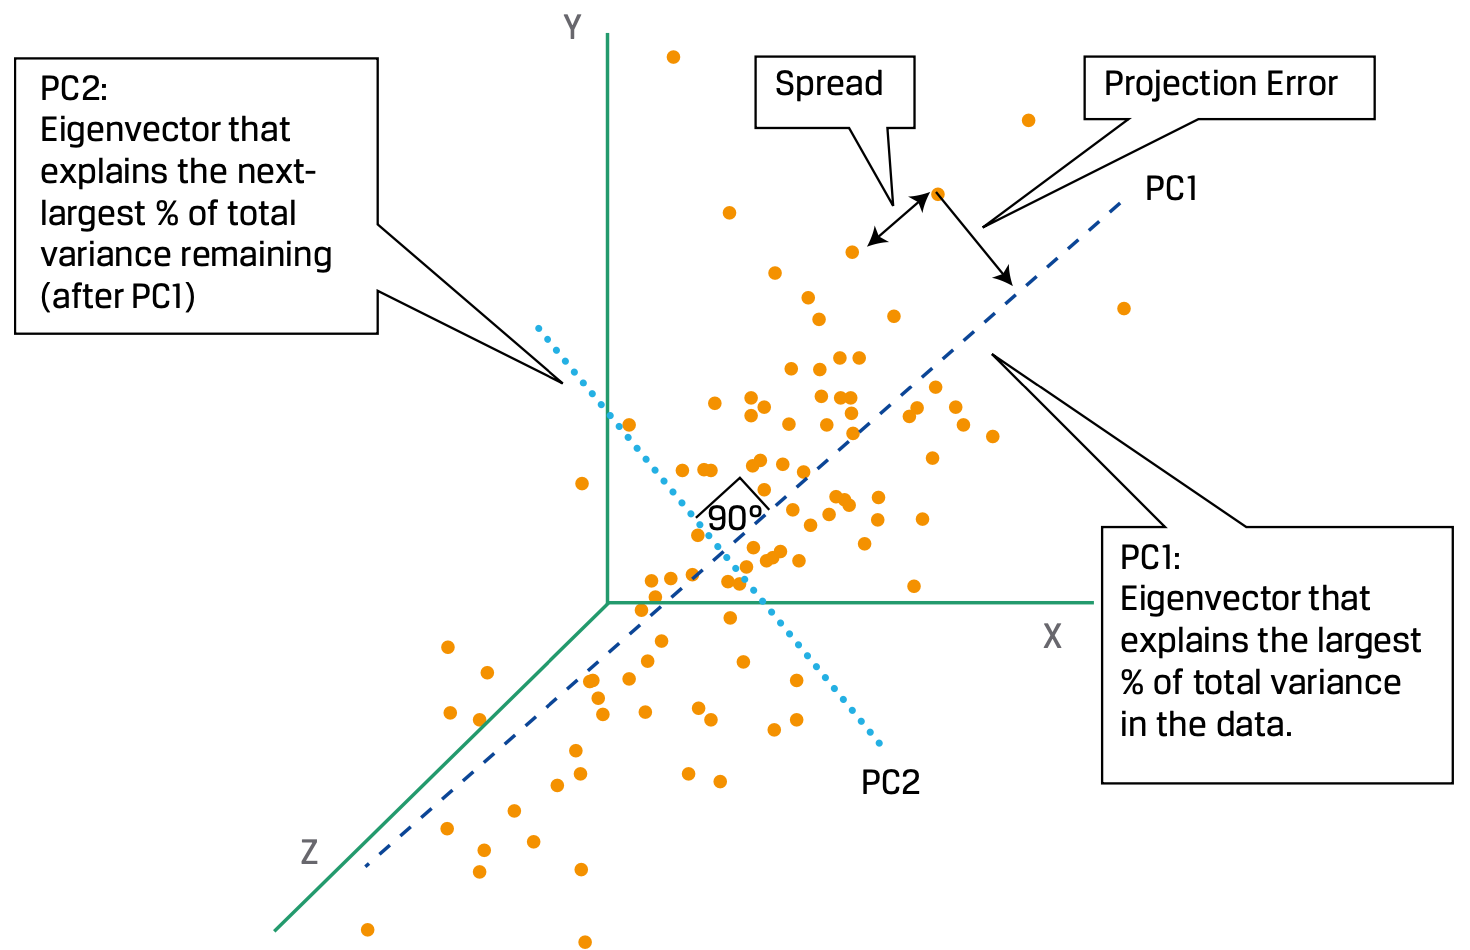
\includegraphics[scale=0.35]{/quant/pca}
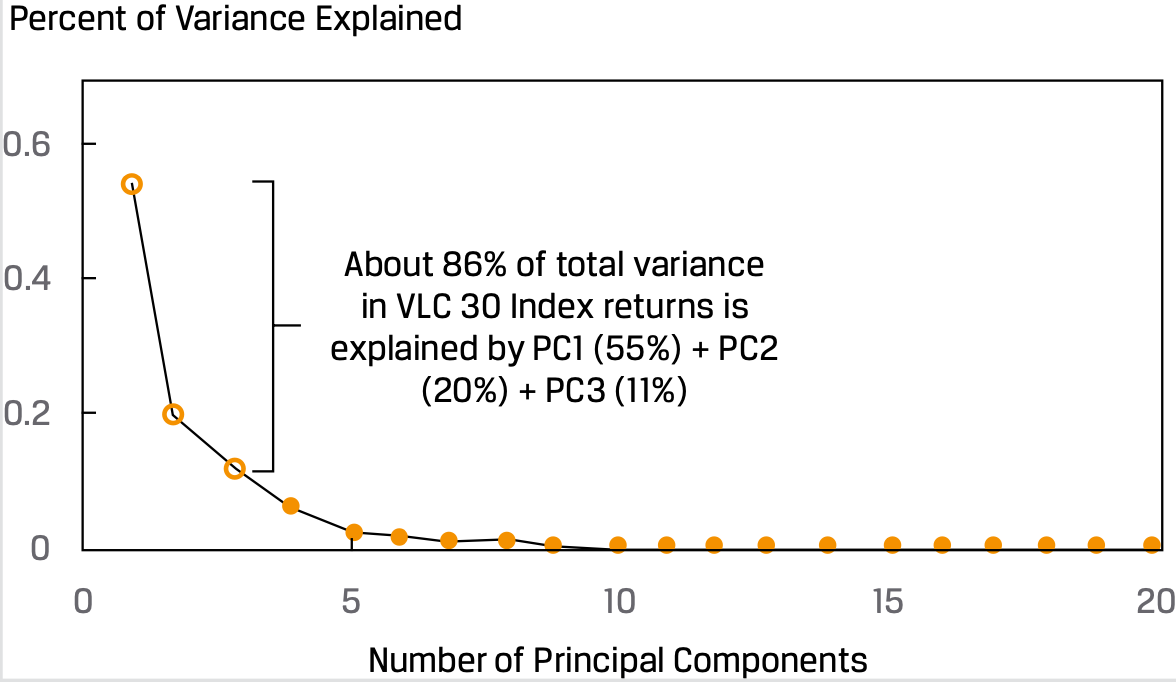
\includegraphics[scale=0.37]{/quant/screeplot}
\caption{PCA and the associated scree plot}
\end{figure}

\begin{definition} \hlt{$K$-Means Clustering}\\
Partitions observations into $k$ non-overlapping clusters, where $k$ is a hyper-parameter.\\
Each cluster has a centroid, each new observation is assigned to a cluster based on its proximity to the centroid.\\
As a new observation gets assigned to a cluster, its centroid is recalculated, which may result in reassignment of some observations, resulting in a new centroid and so forth until all observations are assigned, and no new assignment is made.
\end{definition}

\begin{definition} \hlt{Hierarchical Clustering}\\
Builds a hierarchy of clusters without any predefined number of clusters.\\
May be built bottom-up (agglomerative) or top-down (divisive).\\
Dendrograms may be used to visualise the hierarchical clusters.
\end{definition}

\begin{figure}[H]
\centering
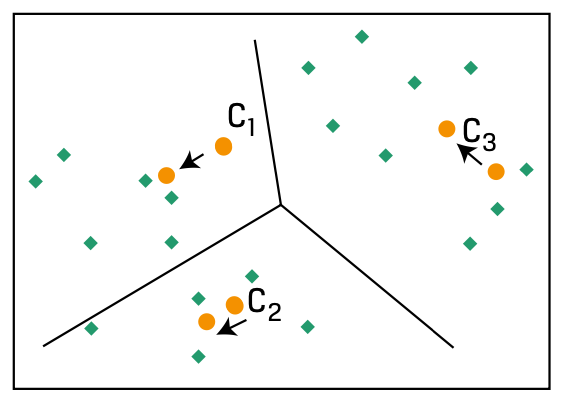
\includegraphics[scale=0.45]{/quant/kmeans}
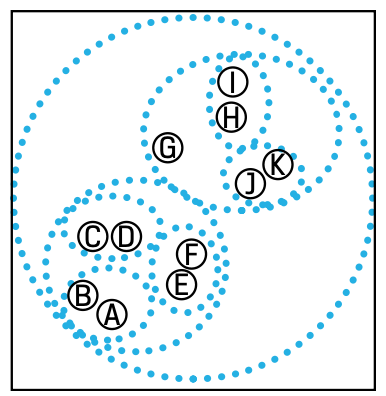
\includegraphics[scale=0.45]{/quant/hcluster}
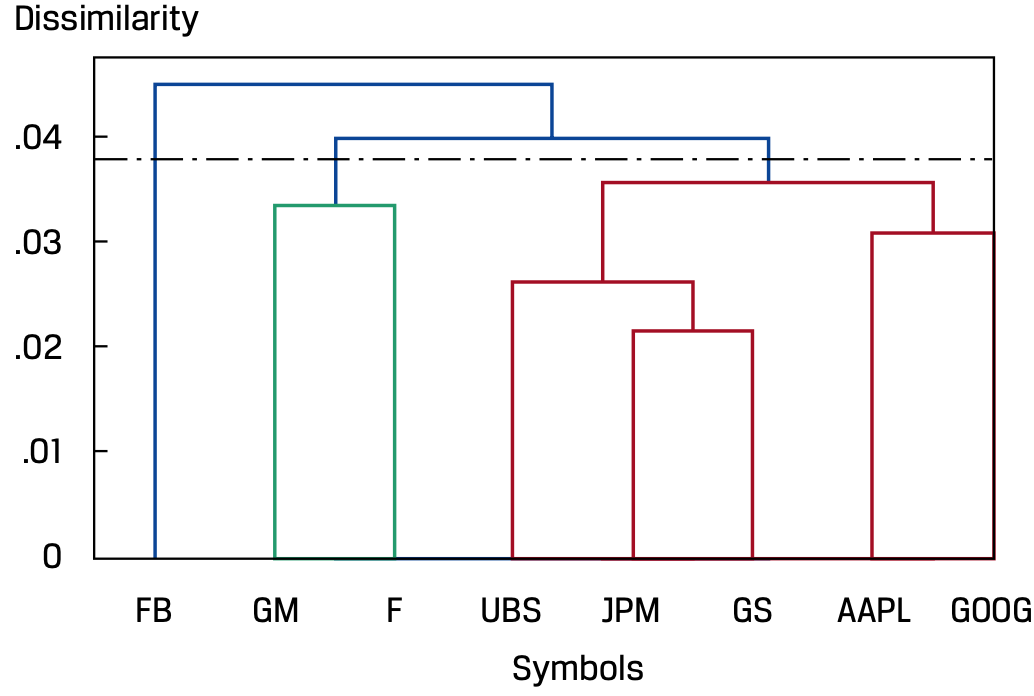
\includegraphics[scale=0.3]{/quant/dendrogram}
\caption{$K$-Means Clustering, Hierarchical Clustering with Dendrogram}
\end{figure}

\begin{definition} \hlt{Neural Networks}\\
Used for classification and regression in supervised learning but are also important in reinforcement learning, which does not require human-labeled training data.\\
Able to model nonlinear relationships between dependent and independent variables.\\
Input layer has nodes equal to dimension (feature set). Hidden layers has nodes with summation operator, activation function. Output layer produces set of probability in target categories. 
\end{definition}

\begin{figure}[H]
\centering
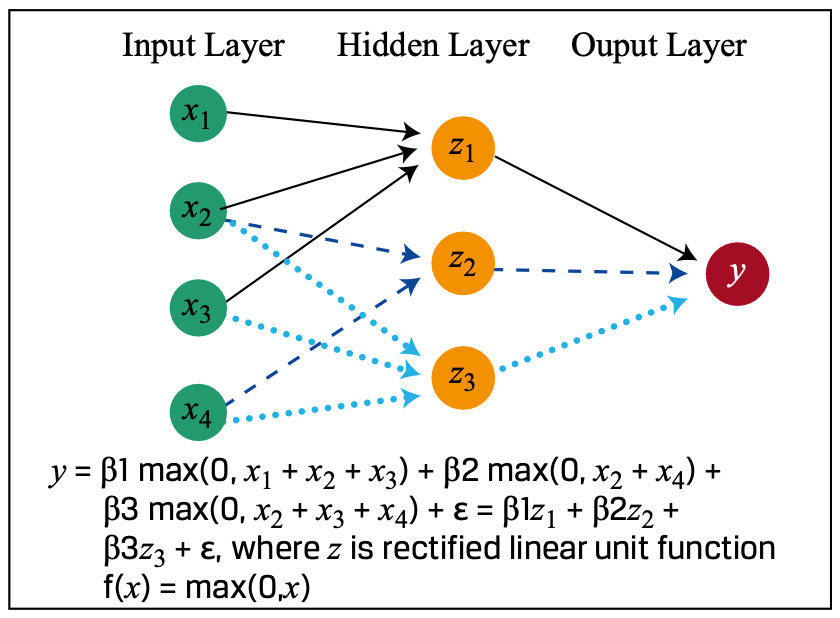
\includegraphics[scale=0.4]{/quant/nn}
\caption{Neural Network}
\end{figure}

\begin{definition} \hlt{Deep Neural Networks (DNNs)}\\
Neural networks with at least $2$ but potentially more than $20$ hidden layers.
\end{definition}

\begin{definition} \hlt{Reinforcement Learning (RL)}\\
Algorithms have an agent that seeks to maximise a defined reward given defined constraints.\\
Does not rely on training data; learns based on feedback from trials. 
\end{definition}

\begin{figure}[H]
\centering
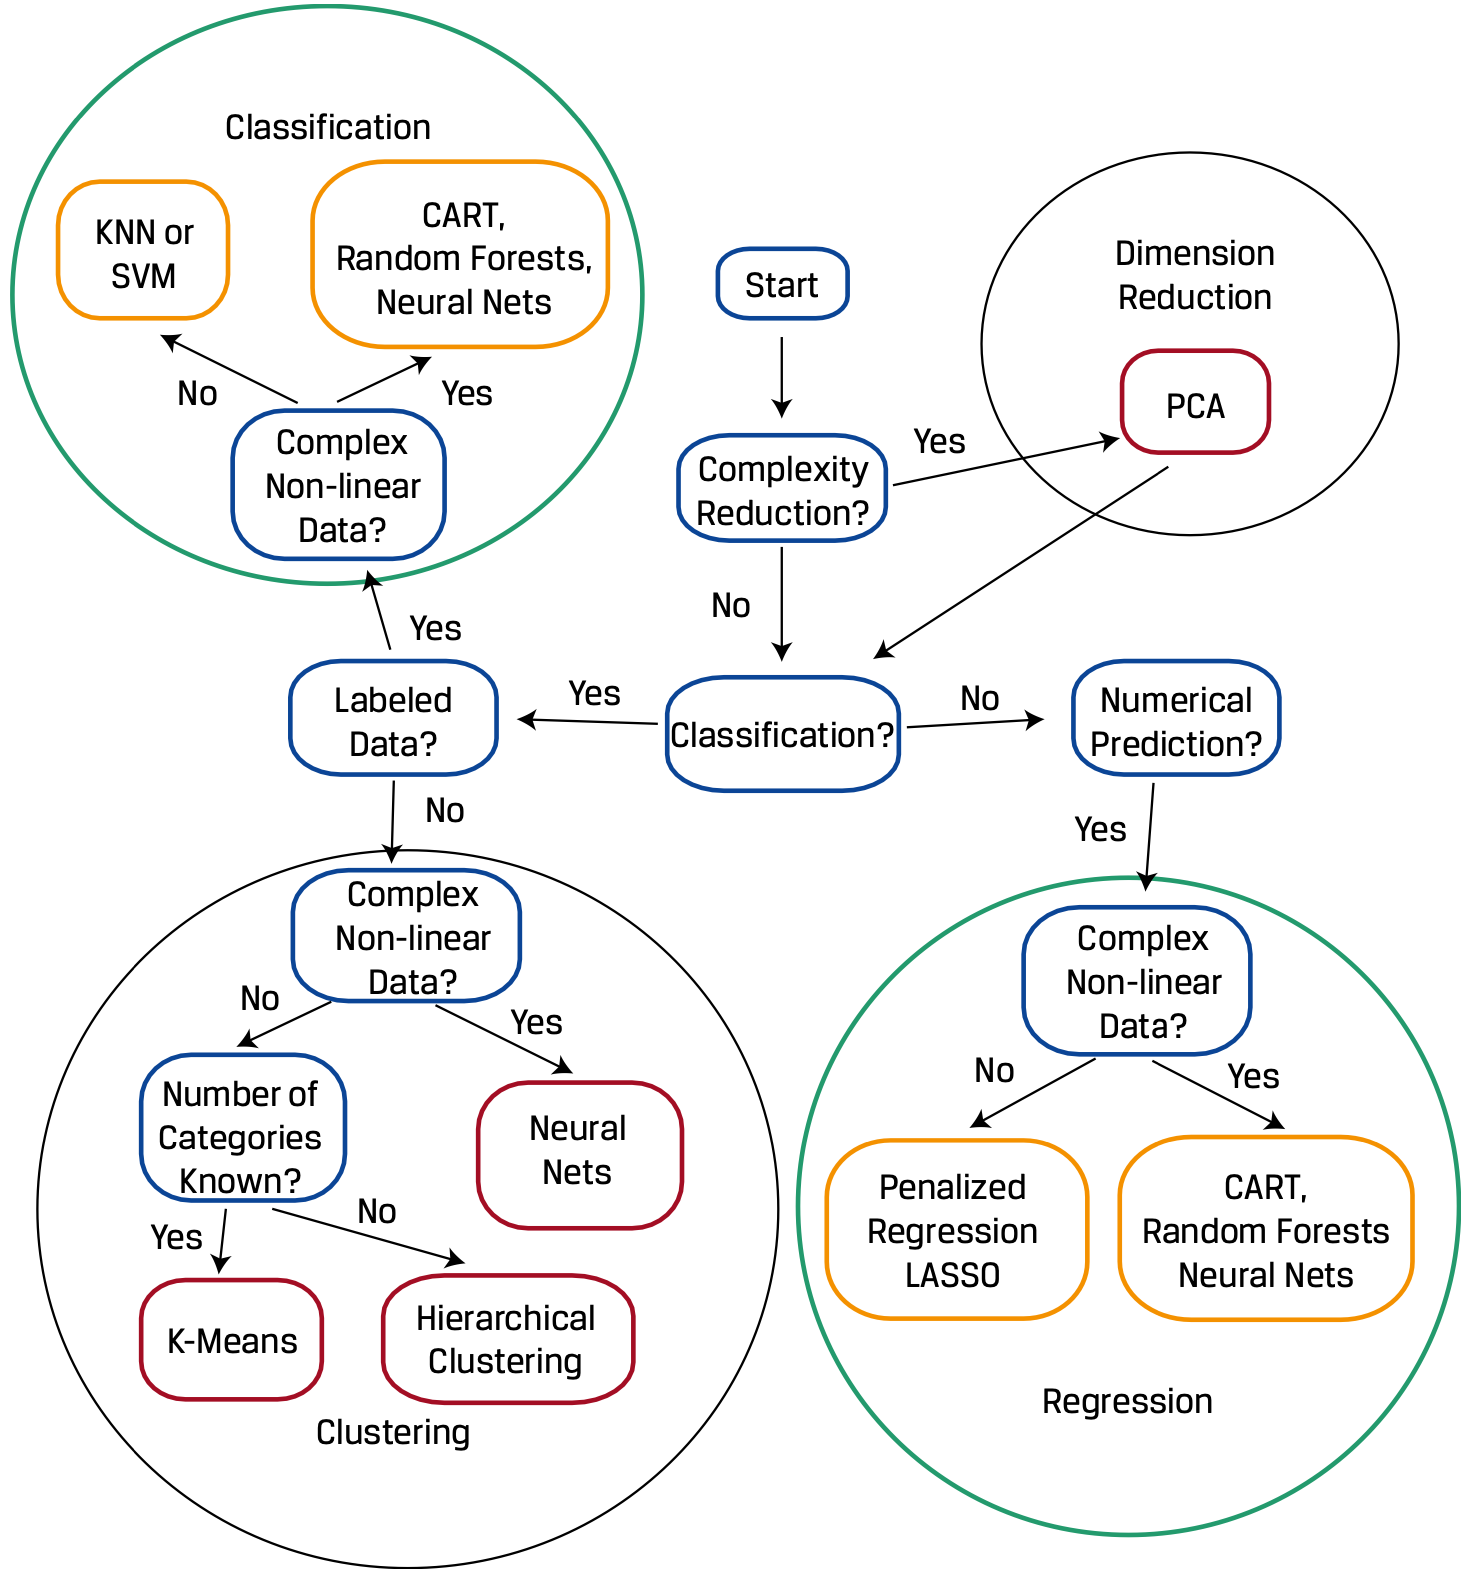
\includegraphics[scale=0.45]{/quant/flowchart}
\caption{Flowchart for choosing ML Algorithms}
\end{figure}


\newpage

\subsection{Big Data Projects}

\begin{remark} \hlt{ML Model Building Steps for Structured Data}
\begin{enumerate}[label=\roman*.]
\setlength{\itemsep}{0pt}
\item Conceptualisation of modelling task: define output, user, usage in existing or new processes
\item Data collection: whether from internal or external source
\item Data preparation and wrangling: cleansing, pre-processing of data
\item Data exploration: Exploratory Data Analysis (EDA), feature selection, feature engineering
\item Model training: select ML method, evaluate performance, tuning model
\end{enumerate}
\end{remark}

\begin{remark} \hlt{ML Model Building Steps for Unstructured Data}
\begin{enumerate}[label=\roman*.]
\setlength{\itemsep}{0pt}
\item Problem formulation: define input and output, usage, purpose
\item Data curation: via web scraping, and annotation of labels.
\item Text preparation and wrangling: convert data to usable format
\item Text exploration: create word clouds, text feature selection and engineering
\end{enumerate}
\end{remark}

\begin{figure}[H]
\centering
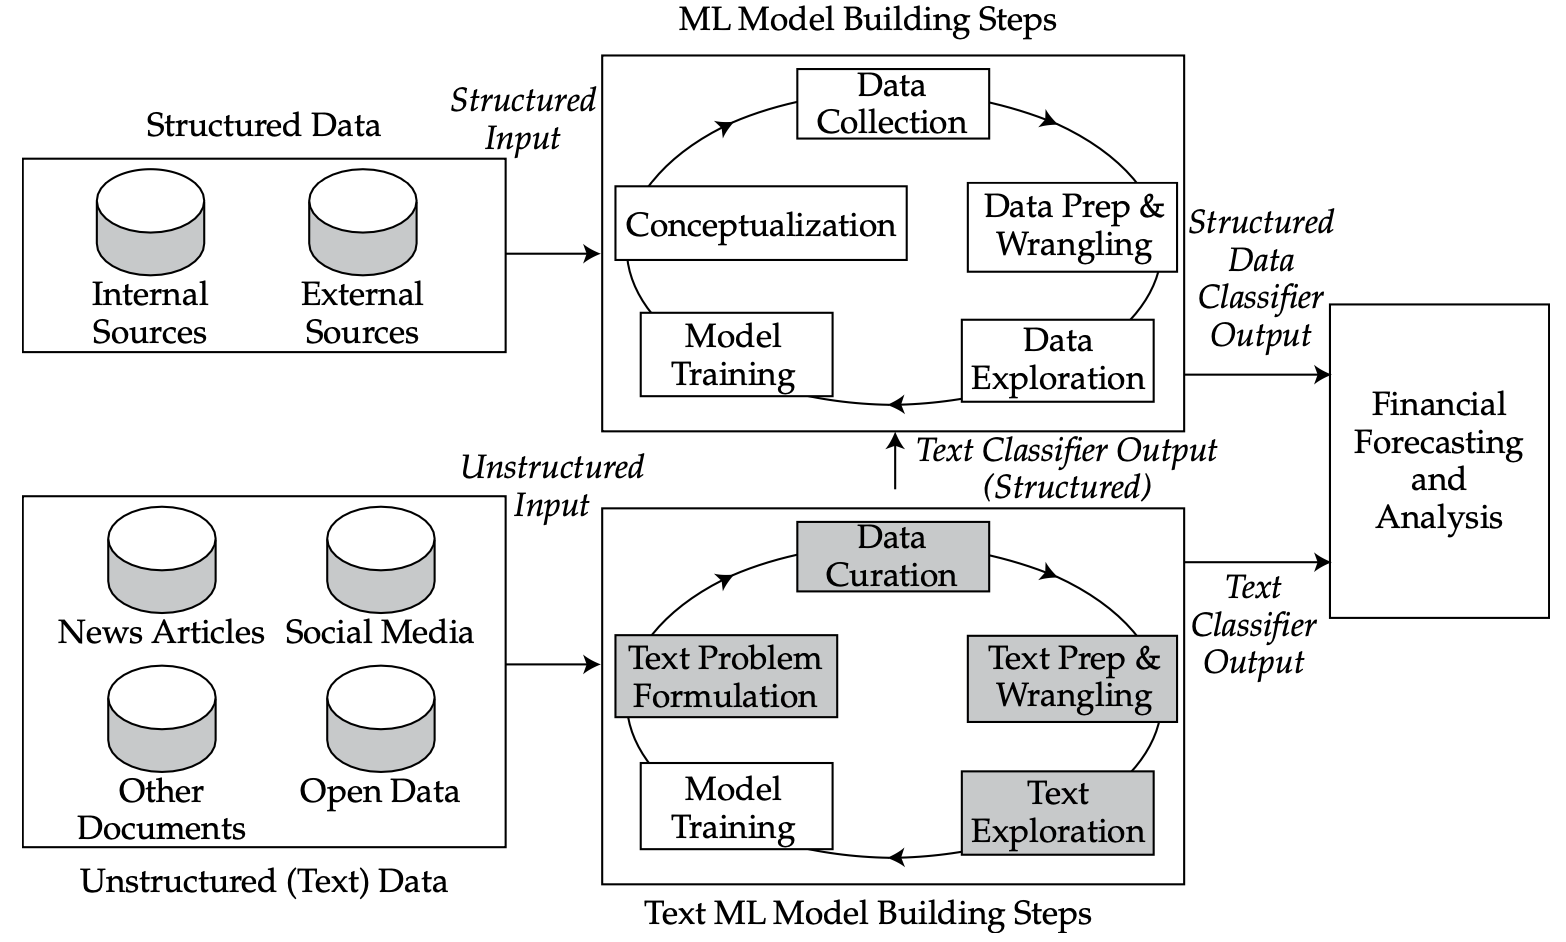
\includegraphics[scale=0.45]{/quant/mlbuild}
\caption{Model building for financial forecasting using big data}
\end{figure}

\begin{definition} \hlt{Data Cleansing}\\
Deals with reducing errors in raw data. Spot incomplete, duplicated, erroneous, or inaccurate values.\\
Metadata (summary data) may serve as starting point for error identification
\end{definition}

\begin{definition} \hlt{Data Wrangling}\\
Preprocessing the data for model use. Includes dealing with outliers, extract useful variables from existing data points, scaling the data, feature selection, aggregation of variables.
\end{definition}

\begin{definition} \hlt{Types of Data Errors and Rectification}
\begin{enumerate}[label=\roman*.]
\setlength{\itemsep}{0pt}
\item Incompleteness error: missing values and NA to be omitted or substituted
\item Invalidity error: data outside of meaningful range. Data to be verified.
\item Inaccuracy error: data not a measure of true value. To be rectified with business records.
\item Inconsistency error: in conflict with rest of data. To clarify with another source.
\item Non-uniformity error: data not in same format. To be converted to same format.
\item Duplication error: to remove duplicate entries.
\end{enumerate}
\end{definition}

\begin{remark} \hlt{Dealing with Outlier Data}
\begin{enumerate}[label=\roman*.]
\setlength{\itemsep}{0pt}
\item Trimming: removing highest and lowest $\alpha \%$ of observations
\item Winsorisation: extreme values replaced by maximum value allowable for that variable
\end{enumerate}
\end{remark}

\begin{remark} \hlt{Conversion of Data Features}
\begin{enumerate}[label=\roman*.]
\setlength{\itemsep}{0pt}
\item Normalisation: scales values between $0$ and $1$.
\begin{equation}
X_i = \frac{X_i - X_{\min}}{X_{\max} - X_{\min}} \nonumber
\end{equation}
\item Standardisation: centres variables at $0$, then scales them as standard deviations from mean.
\begin{equation}
X_i = \frac{X_i - \mu}{\sigma} \nonumber
\end{equation}
\end{enumerate}
Normalisation is sensitive to outliers. Standardisation is less sensitive to outliers
\end{remark}

\begin{method} \hlt{Text Preparation or Cleansing}
\begin{enumerate}[label=\roman*.]
\setlength{\itemsep}{0pt}
\item Remove HTML text using regular expression (regex).
\item Remove punctuations, except percentage, currency symbols, question marks. These to be substituted with annotations to preserve grammatical meaning.
\item Remove numbers and substituted with annotation /number/, except if of interest
\item Remove white spaces
\end{enumerate}
\end{method}

\begin{method} \hlt{Text Tokenisation (Normalisation of Text)}
\begin{enumerate}[label=\roman*.]
\setlength{\itemsep}{0pt}
\item Lowercase all alphabets to remove distinction among the same words
\item Stop words removed to reduce number of tokens in training set, except if critical
\item Stemming: convert inflicted forms of word to its base word. Porter’s algorithm may be used.
\item Lemmatisation: convert inflicted forms of word into its morphological root.
\end{enumerate}
Stemming, lemmatisation reduce repetition of words in various forms.
\end{method}

\begin{remark} \hlt{Output of Text Tokenisation}
\begin{enumerate}[label=\roman*.]
\setlength{\itemsep}{0pt}
\item Bag of words (BOW): collection of distinct set of tokens from all text in sample data
\item Document term matrix (DTM): each row is a document, each column is a token. 
\item N-grams: representation of word sequences. Provide context for advanced ML.
\end{enumerate}
\end{remark}

\begin{method} \hlt{Exploratory Data Analysis (EDA)}\\
Uses visualisation to summarise and observe data. To understand data properties, find patterns and relationships in data, inspect basic questions and hypothesis, document data distribution and characteristics, plan modelling strategies for next steps.
\begin{enumerate}[label=\roman*.]
\setlength{\itemsep}{0pt}
\item Feature selection: only pertinent features selected for training. Statistical measures used to assign a score gauging importance of each feature, then ranked.
\item Feature engineering: create new features by changing, transforming existing features
\item One-hot encoding: convert categorical variables into binary form.
\end{enumerate}
\end{method}

\begin{remark} \hlt{Text Exploration}
\begin{enumerate}[label=\roman*.]
\setlength{\itemsep}{0pt}
\item Term frequency (TF): ratio of number of times token occur, divided by total number of tokens.\\
To prune words with very low and very high TF values so as to remove noise.
\item Document frequency (DF): number of documents that contain token, divide by total document number.
\item Inverse document frequency (IDF): $IDF = \log (1/DF)$, measure how unique a term is.
\item TF-IDF: $=TF \times IDF$. A higher value means more frequent in smaller number of docs, hence indicates a more important word.
TF-IDF value varies by number of documents in dataset, hence performance vary if document number is small. Metric is calculated at the sentence level, not at collection level.
\item Word cloud: visualises the most informative words based on their TF value.
\end{enumerate}
\end{remark}

\begin{remark} \hlt{Feature Selection for Text}
\begin{enumerate}[label=\roman*.]
\setlength{\itemsep}{0pt}
\item Frequency measure used for vocabulary pruning, filter very high and low TF values.
\item $\chi^2$ test applied to test independence of $2$ events: occurrence of token and occur of class.\\
Test ranks tokens by usefulness to each class in text class probability.\\
Tokens with highest $\chi^2$-statistics occur more frequently in texts associated with a class, hence may be used as feature due to higher discriminatory potential.
\item Mutual information (MI) measures how much info is contributed by token to class of text.\\
$MI = 0$ if token distribution in all text class is same.\\
$MI = 1$ if token in any one class tends to occur more often in only that particular class of text.
\end{enumerate}
\end{remark}

\begin{remark} \hlt{Feature Engineering for Text}
\begin{enumerate}[label=\roman*.]
\setlength{\itemsep}{0pt}
\item Numbers: converted to token such as /number/
\item N-grams: multi-word patters that are discriminative identified, with connection intact
\item Name entity recognition (NER): analyse individual token and their surrounding semantics while referring to its dict to tag an object class to the token.\\
Can identify critical tokens on which lowercasing, stemming can be avoided.
\item Parts of speech (POS): tags words as noun, verb, adjective etc.\\
Useful for separating verbs and nouns for text analytics.
\end{enumerate}
\end{remark}

\begin{remark} \hlt{Causes of Model Fitting Errors}
\begin{enumerate}[label=\roman*.]
\setlength{\itemsep}{0pt}
\item Dataset size: small datasets lead to under-fitting the model
\item Number of features: may lead to under-fit or overfit.
\end{enumerate}
\end{remark}

\begin{remark} \hlt{Model Selection Factors}
\begin{enumerate}[label=\roman*.]
\setlength{\itemsep}{0pt}
\item Supervised or unsupervised learning: whether data is labelled/unlabelled, purpose of model
\item Type of data: numeric data use CART, text data use GLM and SVM. Image data use NN ad deep learning. Speech data use deep learning methods.
\item Size of data: type of models used depends on number of features and number of instances of data
\end{enumerate}
\end{remark}

\begin{definition} \hlt{Class Imbalance}\\
Number of instances for one class significantly larger than other classes. Not ideal for supervised learning.\\
Choice of under-sample or oversample depends on context.\\
Advanced techniques may reproduce synthetic data from existing data.
\end{definition}

\begin{flushleft}
Confusion Matrix\\
\begin{tabular}{|c|c|c|}
\hline
\rowcolor{gray!30}
Prediction vs Actual & Class $1$ & Class $0$ \\
\hline
Class $1$ & True Positives (TP) & False Positives (FP), Type I Error\\
\hline
Class $0$ & False Negatives (FN), Type II Error & True Negatives (TN)\\
\hline
\end{tabular}
\end{flushleft}

\begin{definition} \hlt{Model Performance Metrics}
\begin{enumerate}[label=\roman*.]
\setlength{\itemsep}{0pt}
\item Precision: ratio of true positives to all predicted positives.\\
High precision valued when cost of Type I error is large.
\begin{equation}
P = \frac{TP}{TP + FP} \nonumber
\end{equation}
\item Recall: ratio of true positives to all actual positives.\\
High recall valued when cost of Type II error is large.
\begin{equation}
R = \frac{TP}{TP + FN} \nonumber
\end{equation}
\item Accuracy: proportion of correct forecasts out of a total number of forecasts
\begin{equation}
\text{Accuracy} = \frac{TP + TN}{TP + FP + TN + FN} \nonumber
\end{equation}
\item $F1$ Score: harmonic mean of precision and recall.\\
More appropriate to be used when unequal class distribution is present in the dataset.
\begin{equation}
F1 \text{ Score} = \frac{2 \times P \times R}{P + R} \nonumber
\end{equation}
\end{enumerate}
\end{definition}

\begin{definition} \hlt{Receiver Operating Characteristic (ROC)}\\
Plots curve showing trade-off between false positive rate ($x$-axis) and true positive rate ($y$-axis).\\
More convex curve indicates better performance.\\
Area under the curve (AUC): $AUC \rightarrow 1$ is perfect prediction. $AUC \rightarrow 0.5$ is as good as random guess.
\begin{align}
TPR &= \frac{TP}{TP + FN}, \ \ \ FPR = \frac{FP}{FP + TN} \nonumber
\end{align} 
\end{definition}

\begin{figure}[H]
\centering
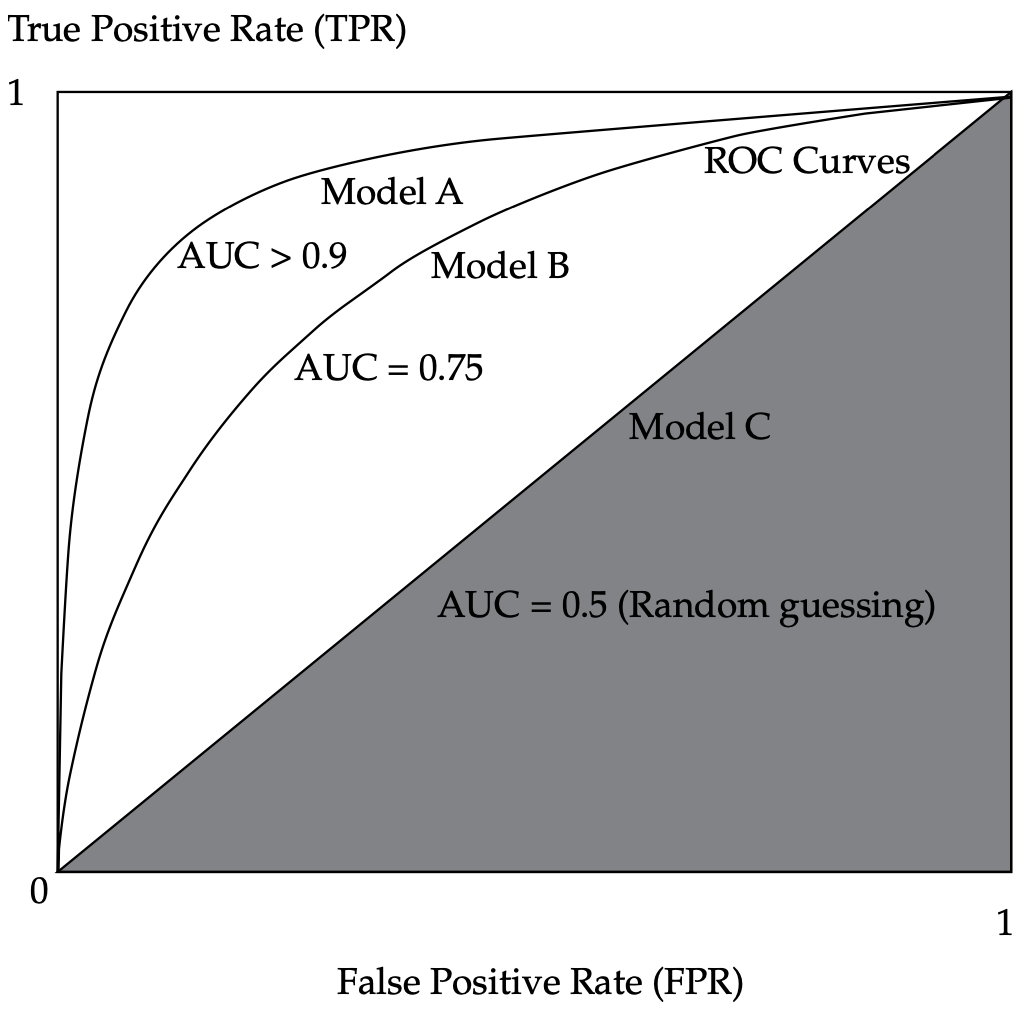
\includegraphics[scale=0.3]{/quant/aucroccurve}
\caption{ROC Curve}
\end{figure}

\begin{definition} \hlt{Root Mean Squared Error (RMSE)}\\
Useful for data predictions that are continuous, such as regression models.\\
The RMSE is a single metric summarising the prediction error in a sample.
$RMSE = \sqrt{\frac{1}{n} \sum\limits_{i=1}^n (\text{Predicted}_i - \text{Actual}_i)^2}$
\end{definition}

\begin{definition} \hlt{Grid Search}\\
Systematically train ML model using different combination of hyper-parameter values to determine combination of values that has best model performance.
\end{definition}

\begin{definition} \hlt{Regularisation}\\
Slight regularisation lightly penalises model complexity, thereby allowing most or all of the features to be included in the model and thus potentially enabling the model to memorise the data.\\
Large regularisation excessively penalises model complexity, thereby allowing too few of the features to be included in the model and causing the model to learn less from the data.\\
Optimum regularisation minimises both variance and bias errors in a balanced fashion. 
\end{definition}

\begin{figure}[H]
\centering
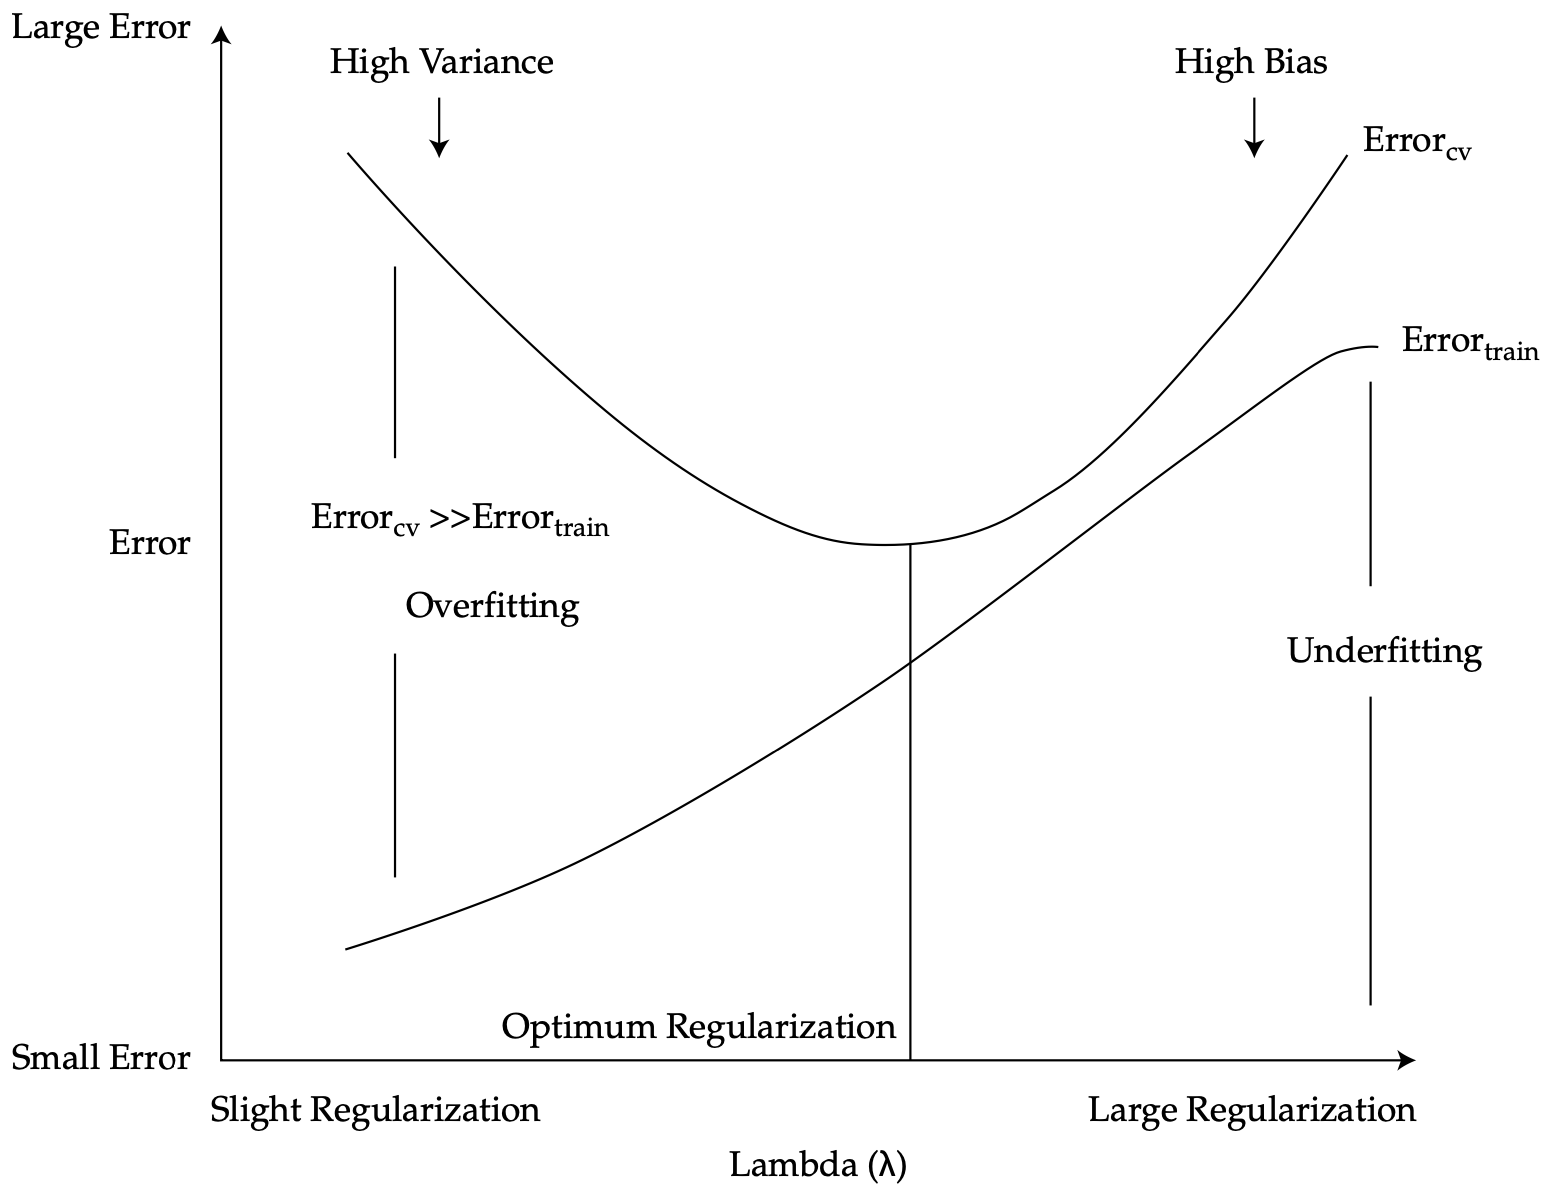
\includegraphics[scale=0.3]{/quant/hypparamfitcurve}
\caption{Fitting Curve for Regularisation Hyper-parameter $\lambda$}
\end{figure}

\begin{definition} \hlt{Ceiling Analysis}\\
Systematic process of evaluating different components in the pipeline of model building.\\
Determine which sub-model needs to be tuned to improve the overall accuracy of the larger model.
\end{definition}







\newpage

\section{Economics}

\subsection{Currency Exchange Rates}

\begin{definition} \hlt{Exchange Rate}\\
Price of one currency in terms of another.\\
Typically quoted as 'Price/Base' notation, i.e., $1.650$ USD/EUR means $1$ EUR cost $1.650$ USD.
\begin{enumerate}[label=\roman*.]
\setlength{\itemsep}{0pt}
\item Spot exchange rate: for immediate delivery, with $T+2$ settlement (except CAD/USD, with $T+1$)
\item Forward exchange rate: to be done in future.
\end{enumerate}
\end{definition}

\begin{remark} \hlt{Dealer Quotes}\\
Quoted as 'Bid-Ask', where bid price is price at which dealer will buy, ask is price at which dealer sells.
\end{remark}

\begin{remark} \hlt{Foreign Exchange Spread}\\
Difference between offer and bid price is the spread, quoted as 'pips', which is $1/10,000$ of a dollar.\\
Ask Price $>$ Bid Price. Bid-offer spread from dealer is wider than the spread dealer receives from interbank.
\end{remark}

\begin{remark} \hlt{Dealer Spread Factors}
\begin{enumerate}[label=\roman*.]
\setlength{\itemsep}{0pt}
\item Spread in interbank market: spreads vary directly with spreads quoted in interbank market.
\item Size of transaction: large, liquidity-demanding transactions get quoted larger spread.
\item Relationship between dealer and client: dealer give favourable rates to preferred clients based on other ongoing business relationships.
\end{enumerate}
\end{remark}

\begin{remark} \hlt{Interbank Spread Factors}
\begin{enumerate}[label=\roman*.]
\setlength{\itemsep}{0pt}
\item Currencies traded: high-volume currency pairs command lower spreads than lower-volume pairs
\item Time of day: most liquid when major trading centres are open (Asian session not as liquid as London, NY sessions). Spreads are narrower when both NY, London sessions are open.
\item Market volatility: higher volatility due to geopolitical events, market crashes, major data releases will lead to wider spreads. Spreads change over time in response to volatility changes.
\end{enumerate}
\end{remark}

\begin{remark} \hlt{Forward Exchange Rate Spreads}\\
Spreads in forward exchange rate quotes increase with maturity, as:
\begin{enumerate}[label=\roman*.]
\setlength{\itemsep}{0pt}
\item longer maturity contracts tend to be less liquid,
\item counterparty credit risk in forward contracts increase with maturity,
\item interest rate risk in forward contracts increase with maturity
\end{enumerate} 
\end{remark}

\begin{remark} \hlt{Tips with Foreign Transaction Quotes}
\begin{enumerate}[label=\roman*.]
\setlength{\itemsep}{0pt}
\item For transactions in base currency, buy base currency at ask, sell base currency at bid.
\item For transactions in price currency, buy price currency at bid, sell price currency at ask.
\item Alternatively, follow the up-the-bid-and-multiply, down-the-ask-and-divide rule.\\
i.e., given USD/AUD, to convert USD into AUD, use ask (going down the quote).\\
To convert AUD to USD, use bid (going up the quote).
\end{enumerate}
\end{remark}

\begin{definition} \hlt{Cross Rate}\\
Exchange rate between two currencies implied by exchange rates with a common third currency.\\
To use cross rates when there is no active FC market in currency pair considered.
\end{definition}

\begin{remark} \hlt{Cross Rates with Bid-Ask Spreads}\\
Bid-ask spreads complicate the computation of cross rates. Suppose we have currencies $A,B,C$.
\begin{align}
\left(\frac{A}{C} \right)_{\text{Bid}} &= \left(\frac{A}{B} \right)_{\text{Bid}} \times \left(\frac{B}{C} \right)_{\text{Bid}}, \ \ \ \ \ \ \ \ \ \ \left(\frac{A}{C} \right)_{\text{Offer}}  = \left(\frac{A}{B} \right)_{\text{Offer}} \times \left(\frac{B}{C} \right)_{\text{Offer}} \nonumber
\end{align}
If given instead $A/B$ and $C/B$ rates, make adjustments to obtain $B/C$ bid and offer rates from $C/B$ bid and offer rates, as $A/B \times C/B \neq A/C$. Process is
\begin{align}
\left(\frac{B}{C} \right)_{\text{Bid}} = \frac{1}{\left(\frac{C}{B} \right)_{\text{Offer}}}, \ \ \ \ \ \ \ \left(\frac{B}{C} \right)_{\text{Offer}} = \frac{1}{\left(\frac{C}{B} \right)_{\text{Bid}}} \nonumber
\end{align}
\end{remark}

\begin{method} \hlt{Triangular Arbitrage}\\
Begin with tree pairs of currencies, each with bid-ask quotes, construct a triangle where each node in triangle represents one currency. To check for arbitrage, go around the triangle clockwise (and counterclockwise) until starting point. Follow the up-the-bid-and-multiply, down-the-ask-and-divide rule.\\
Only one direction is profitable; cannot earn arbitrage profit in both directions.
\end{method}

\begin{figure}[H]
\centering
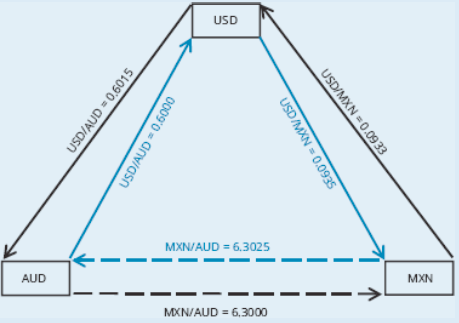
\includegraphics[scale=0.5]{/econ/trianglearb}
\caption{Example of triangle arbitrage, only blue is profitable}
\end{figure}

\begin{definition} \hlt{Forward Rates}\\
Currency is quoted at forward premium (discount) relative to second currency if forward price is greater (less) than spot price. The premium or discount is for the base currency.
\begin{equation}
\text{Forward Premium} = F_{f/d} - S_{f/d} \nonumber
\end{equation}
In FX markets, forward quotes are presented as premium or discount over spot rates.\\
Note, spot rate $S_{f/d}$ is mid-market of bid-offer spread.
\end{definition}

\begin{remark} \hlt{Mark-to-Market Value}\\
Value of forward contract prior to expiration is also known as mark-to-market value.\\
Take difference between forward price locked-in and currency forward price, multiply that by size of contract, then discount for time remaining until contract settlement date.
\begin{equation}
V_t = \frac{(F_t - F_0)(\text{Contract Size})}{1 + i_f(\frac{n}{360})} \nonumber
\end{equation}
where $i_f$ is interest rate (MRR) of price currency, $n$ is days remaining to maturity of contract ($T-t$).\\
Note the forward price is to sell base currency, and MRR is market reference rate.
\end{remark}

\subsubsection{International Parity Conditions}

\begin{remark} \hlt{Relationship of Forward Rate to Spot Rates}\\
Given one unit of domestic currency, two investment choices may be made:
\begin{enumerate}[label=\roman*.]
\setlength{\itemsep}{0pt}
\item Invest in cash for $1$ year at domestic risk-free rate to earn $1 + i_d$.
\item Convert domestic currency to foreign currency at spot rate $S_{f/d}$, invest for one year at foreign risk-free rate $i_f$, then at end of period, will have $S_{f/d}(1+i_f)$ units of foreign currency.\\
Convert back at forward rate of $F_{f/d}$, then we would have $S_{f/d}(1+i_f)(1/F_{f/d})$ units of domestic currency.
\end{enumerate}
As both are risk free, should offer same return, hence we have the relationship
\begin{equation}
(1+i_d) = S_{f/d} (1+i_f) \left( \frac{1}{F_{f/d}} \right) \nonumber
\end{equation}
\end{remark}

\begin{definition} \hlt{Covered Interest Rate Parity}\\
'Covered' means bound by arbitrage; arbitrage force forward contract exchange rate to a level consistent with difference between two country's nominal interest rates.\\
Parity holds when any forward premium or discount exactly offsets differences in interest rates, hence investor would earn the same return in either currency.\\
If foreign interest rates are higher than local interest rates, the forward discount on foreign currency relative to local currency will just offset the higher foreign interest rate.
\begin{align}
F_{f/d} = S_{f/d} \left( \frac{1 + i_f (\frac{n}{360})}{1 + i_d (\frac{n}{360})} \right), \ \ \ \ \ \  \text{Forward Premium} = F_{f/d} -  S_{f/d} = S_{f/d} \left( \frac{(\frac{n}{360})}{1 + i_d (\frac{n}{360})} \right) (i_f - i_d) \nonumber
\end{align}
\end{definition}

\begin{definition} \hlt{Uncovered Interest Rate Parity}\\
'Uncovered' means not bound by arbitrage. If forward contracts are not available, or if capital flows are restricted so as to prevent arbitrage, then the relationship need not hold.\\
Given $f/d$, the base currency $d$ is expected to appreciate by approximately $i_f - i_d$.
\begin{equation}
\% \Delta S^e_{f/d} = i_f - i_d \nonumber
\end{equation}
where $\% \Delta S^e_{f/d}$ is change in spot rate expected.\\
There is no reason that uncovered interest rate parity must hold in short run.\\
There is evidence that it does generally hold in the long-run, hence longer-term expected future spot rate based on uncovered parity are often used as future exchange rate forecasts.
\end{definition}

\begin{remark} \hlt{Covered vs Uncovered Interest Rate Parity}
\begin{enumerate}[label=\roman*.]
\setlength{\itemsep}{0pt}
\item Covered parity derives the no-arbitrage forward rate, while uncovered parity derives the expected future spot rate (which is not market traded).
\item Under uncovered parity, if foreign interest rate is higher, foreign currency is expected to depreciate by approximately same amount, hence investor is indifference between investing in foreign or domestic currency. An investor that chooses to invest to foreign currency without additional return is not demanding a risk premium for foreign currency risk. Hence uncovered parity assumes investor is \hlt{risk-neutral}.
\end{enumerate}
\end{remark}

\begin{definition} \hlt{Forward Rate Parity}\\
If covered interest rate parity holds, and uncovered interest rate parity also holds; where the no-arbitrage forward rate equals the expected future spot rate.
\begin{equation}
\frac{F_{f/d} - S_{f/d}}{S_{f/d}} = \% \Delta S^e_{f/d} = i_f - i_d \nonumber
\end{equation}
Hence $F_{f/d} = S_{f/d, t}^e$. The forward rate is an unbiased predictor of future spot rate.
\end{definition}

\begin{definition} \hlt{(Domestic) Fisher Relation}\\
Nominal rate of return is approximately the sum of real rate and expected rate of inflation.
\begin{equation}
i = r + \pi^e \nonumber
\end{equation}
\end{definition}

\begin{definition} \hlt{Real Interest Rate Parity}\\
Real interest rates will converge to same level across different markets.
\begin{equation}
r_f - r_d = 0 \nonumber
\end{equation}
\end{definition}

\begin{definition} \hlt{International Fisher Effect}\\
Taking domestic fisher relation and real interest rate parity together; difference between two countries' nominal interest rates should be equal to difference between their expected inflation rates.
\begin{equation}
i_f - i_d = \pi_f^e - \pi_d^e \nonumber
\end{equation}
Argument for equality of real interest rates across countries is based on idea that free capital flows, funds will move to a country with higher real rate until real rates are equalised.
\end{definition}

\begin{definition} \hlt{Law of One Price}\\
Identical goods should trade at the same price across countries when valued in terms of a common currency.
\end{definition}

\begin{definition} \hlt{Absolute Purchasing Power Parity (Absolute PPP)}\\
Compares average price of representative basket of consumption goods between countries using an index.\\
Requires only that the law of once price be correct on average. Assumes goods arbitrage will equate prices of all goods and services across countries.
\begin{equation}
S_{f/d} = \frac{P_f}{P_d} \nonumber
\end{equation}
In practice, even of law of one price holds, absolute PPP might not hold as weights (consumption patterns) of various goods in two economies may not be the same.
\end{definition}

\begin{definition} \hlt{Relative Purchasing Power Parity (Relative PPP)}\\
Changes in exchange rates should exactly offset the price effects of any inflation differential between two countries. Assumes transaction costs and other trade impediments are constant over time.
\begin{equation}
\% \Delta S_{f/d} = \pi_f - \pi_d \nonumber
\end{equation}
Based on idea that even if absolute PPP does not hold, there may still be a relationship between changes in exchange rate and differences between inflation rates of two countries.\\
As there is no true arbitrage available to force relative PPP to hold, violations of relative PPP in short run are common. However, evidence suggests that relative PPP holds approximately in the long-run, and remains a useful method for estimating relationship between exchange rates and inflation rates.
\end{definition}

\begin{definition} \hlt{Ex-Ante Purchasing Power Parity (Ex-Ante PPP)}\\
Same as relative PPP, except it uses expected inflation instead of actual inflation.\\
Countries with persistently high inflation rates should expect to see their currencies depreciate.
\begin{equation}
\% \Delta S_{f/d}^e = \pi_f^e - \pi_d^e \nonumber
\end{equation}
\end{definition}

\begin{figure}[H]
\centering
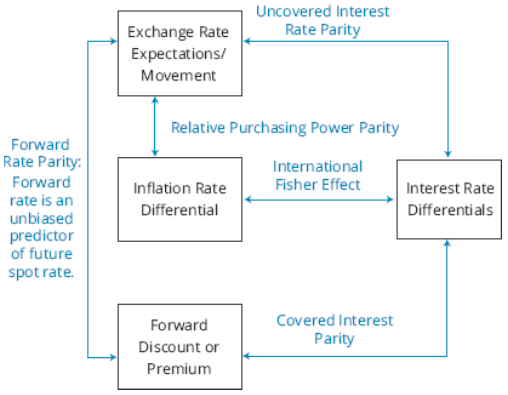
\includegraphics[scale=0.523]{/econ/intparity}
\caption{Relationship between international parity conditions}
\end{figure}

\begin{remark} \hlt{Summary of International Parity Conditions}
\begin{enumerate}[label=\roman*.]
\setlength{\itemsep}{0pt}
\item Covered interest rate parity: arbitrage ensures nominal i/r spread = \% forward premium
\item Uncovered interest rate parity: expected $\% \Delta$ spot rate = nominal i/r spread
\item If covered and covered parity holds, then forward rate is unbiased predictor of future spot rate
\item Ex ante PPP: expected $\Delta$ spot rate = expected diff in domestic and foreign i/r
\item Fisher effect: nominal i/r = real i/r $+$ expected inflation rate; real i/r parity holds
\item International fisher effect: nominal yield spread $=$ domestic and foreign i/r expected inflation differential
\item If ex ante PPP, international fisher effect hold, then expected inflation diff = expected change in exchange rate and nominal i/r differential.\\
Relationship implies expected $\Delta$ exchange rate $=$ nominal i/r diff (uncovered i/r parity)
\end{enumerate}
\end{remark}

\begin{remark} \hlt{Observations of Relationship of Parity Conditions}
\begin{enumerate}[label=\roman*.]
\setlength{\itemsep}{0pt}
\item Covered interest rate parity holds by arbitrage. If forward rate parity holds, uncovered interest rate parity also holds (and vice versa)
\item Interest rate differentials should mirror inflation differentials. This holds true if the international Fisher relation holds. If that is true, can also use inflation differentials to forecast future exchange rates, which is the premise of ex-ante PPP.
\item If ex-ante PPP and international Fisher relation both hold, uncovered interest rate parity will also hold.
\end{enumerate}
\end{remark}

\begin{remark} \hlt{All Parity Condition Holds}\\
If all key international parity conditions hold at all times, $\Delta$ spot rate equals:
\begin{enumerate}[label=\roman*.]
\setlength{\itemsep}{0pt}
\item forward premium or discount (in percentage terms)
\item nominal yield spread between countries
\item difference between expected national inflation rates
\end{enumerate}
Impossible for global investor to earn consistent profit on forex movements.
\end{remark}

\begin{definition} \hlt{FX Carry Trade}\\
Long high-yield currencies, short low-yield currencies. Bets that high-yield currencies have not depreciated and low-yield currencies have not appreciated to levels predicted by interest rate differentials.\\
Strategy can be executed as uncovered interest parity does not hold over short, medium term periods.\\
Strategy attempts to capture interest rate differential, and is a bet against uncovered interest rate parity.\\
Carry trades perform well in low-volatility periods. Higher yields attract larger capital flows, lead to economic boom and appreciation of higher-yield currency, hence earning currency appreciation and interest rate spread. 
\end{definition}

\begin{remark} \hlt{Risks of FX Carry Trade}\\
Risk is that the funding currency may appreciate significantly against investment currency, leading to loss.\\
Return distribution is not normal, with negative skewness and excess kurtosis (fat tails), hence there is a high probability of a large loss (crash risk), this stems from carry trade's leveraged nature.
\end{remark}

\subsubsection{Central Bank Influence}

\begin{definition} \hlt{Balance-of-Payments (BOP) Accounting}\\
Method used to keep track of transactions between country and trading partners.\\
Includes government transactions, consumer transactions, and business transactions.\\
Accounts reflect all payments and liabilities to and from foreigners.
\end{definition}

\begin{definition} \hlt{Current Account}\\
Measures exchange of goods and services, investment income, and unilateral transfers (gifts).
\end{definition}

\begin{definition} \hlt{Financial Account}\\
Measures the flow of funds for debt and equity investment into and out of the country.
\end{definition}

\begin{remark} \hlt{Relationship between Current Account and Capital Account}\\
With current account deficit, to generate a surplus in capital account (or currency will depreciate).\\
Capital flows tend to be the dominant factor influencing exchange rates in the short term, as capital flows tend to be larger and more rapidly changing than goods flows.
\end{remark}

\begin{remark} \hlt{Current Account Influences on Exchange Rates}
\begin{enumerate}[label=\roman*.]
\setlength{\itemsep}{0pt}
\item Flow Supply/Demand Channel: if country sold more goods and services than it purchased (current account surplus), demand for currency should rise, hence appreciate.\\
Assumes trade imbalances will be corrected as deficit country’s currency depreciates.\\
Amount by which exchange rate adjusts depends on
\begin{enumerate}[label=\arabic*.]
\setlength{\itemsep}{0pt}
\item Initial surplus: larger surplus requires larger appreciation of domestic currency
\item Influence of exchange rates on domestic import and export prices
\item Price elasticity of demand of traded goods 
\end{enumerate}
\item Portfolio Balance Channel: country with current account surpluses have capital account deficits, which are investments in countries with current account deficits. Due to flows of capital, investor countries portfolio composition is dominated by few investee currencies. When investor rebalance portfolios, it may have significant negative impact on value of investee country currencies.
\item Debt Sustainability Channel: country with current account deficit is running a current account surplus by borrowing from abroad. When level of debt is too high relative to GDP, investors may question sustainability of debt level, leading to rapid depreciation of borrower currency.
\end{enumerate}
\end{remark}

\begin{remark} \hlt{Capital Account Influences on Exchange Rates}\\
As capital flows into country, demand for currency increases, resulting in appreciation.\\
Higher relative real rates of return attract foreign capital. Capital flows into a country may be needed to overcome shortage of internal savings to fund investments. However, capital flows in excess of needed investment capital pose several problems:
\begin{enumerate}[label=\roman*.]
\setlength{\itemsep}{0pt}
\item Excessive real appreciation of the domestic currency,
\item Financial asset and/or real estate bubbles.
\item Increases in external debt by businesses or government. 
\item Excessive consumption in the domestic market fuelled by credit.
\end{enumerate}
Emerging market governments counteract excessive capital inflows by imposing capital controls or by direct intervention in the foreign exchange markets.
\end{remark}

\begin{definition} \hlt{Mundell-Fleming Model}\\
Model evaluates the short-term impact of monetary and fiscal policies on interest rates, exchange rates.\\
Assumes there is sufficient slack in economy to handle changes in aggregate demand, and inflation is not concern.\\
Changes in inflation rates play no role in exchange rate determination.
\end{definition}

\begin{remark} \hlt{Mundell-Fleming Model: Flexible Exchange Rate Regimes}\\
Rates are determined by supply and demand in FX markets. 
\begin{enumerate}[label=\roman*.]
\setlength{\itemsep}{0pt}
\item High Capital Mobility:
\begin{enumerate}[label=\arabic*.]
\setlength{\itemsep}{0pt}
\item Expansionary monetary policy reduce interest rate, and hence reduce inflow of capital investment in physical and financial assets, hence reduces demand for domestic currency, resulting in appreciation of domestic currency. Vice versa for restrictive monetary policy.
\item Expansionary fiscal policy increase government borrowing and hence increase interest rates, attracting foreign investment, improve financial account, increase demand for currency. Vice versa for restrictive.
\end{enumerate}
\item Low Capital Mobility: impact of trade imbalance on exchange rates is greater than impact of interest rates. Expansionary fiscal or monetary policy leads to increases in net imports, leading to depreciation.
\end{enumerate}
\end{remark}

\begin{flushleft}
Monetary and Fiscal Policy and Exchange Rates
\begin{tabularx}{\textwidth}{p{10em}|p{10em}|X|X}
\hline
\rowcolor{gray!30}
Monetary Policy & Fiscal Policy & High Capital Mobility & Low Capital Mobility\\
\hline
Expansionary & Expansionary & Uncertain & Depreciation\\
\hline
Expansionary & Restrictive & Depreciation & Uncertain\\
\hline
Restrictive & Expansionary & Appreciation & Uncertain\\
\hline
Restrictive & Restrictive & Uncertain & Appreciation\\
\hline
\end{tabularx}
\end{flushleft}

\begin{remark} \hlt{Mundell-Fleming Model: Fixed Exchange Rate Regime}\\
Expansionary monetary policy will lead to depreciation of domestic currency. Government to purchase own currency in FX market, reversing the expansionary stance.\\
Hence, governments cannot both management exchange rates and pursue independent monetary policy. If government wants to manage 
\end{remark}

\begin{definition} \hlt{Monetary Approach to Exchange Rate Determination}\\
Assume that output is fixed, so monetary policy primarily affects inflation, which affects exchange rates.
\begin{enumerate}[label=\roman*.]
\setlength{\itemsep}{0pt}
\item Pure Monetary Model: PPP holds at any point in time, output is held constant. Expansionary monetary policy results in $x \% \uparrow$ money supply, hence  $x \% \uparrow$ in price levels, and an  $x \%$ depreciation of currency.\\
Approach does not take into account expectations on future monetary expansion or contraction.
\item Dornbusch Overshooting Model: assumes prices are sticky in short term, hence do not immediately reflect changes in monetary policy (PPP does not hold in short term). Exchange rates will overshoot long-run PPP value in short term. Expansionary monetary policy increase prices, but in over time leads to a decrease in interest rates, and a larger-than-PPP-implied depreciation of domestic currency due to capital inflows. In long run, exchange rates gradually increase towards PPP implied values.
\end{enumerate}
\end{definition}

\begin{definition} \hlt{Portfolio Balance Approach to Exchange Rate Determination}\\
Approach focuses on the long-term effects of fiscal policy only, and evaluates effects of a sustained fiscal deficit or surplus on currency values.\\
When government runs fiscal deficit, money is borrowed from investors.\\
Investors evaluate debt based on expected risk and return; return is earned on both debt's yield and currency return. Long-term expansionary fiscal policy leads to growing government budget deficit, increasing supply of domestic bonds; investors will continue to purchase the bonds if there is sufficient expected return.\\
However, continued increases in fiscal deficits are unsustainable; investors may refuse to fund the deficits, leading to currency deprecation.
\end{definition}

\begin{remark} \hlt{Combination of Mundell-Flemming and Portfolio Balance Approach}\\
In short term, with free capital flows, expansionary fiscal policy leads to domestic currency appreciation (with higher interest rates). In long term, government has to use tighter fiscal policy, leading to depreciation of domestic currency; else, it would have to use monetary expansion, also leading to depreciation of currency.
\end{remark}

\begin{remark} \hlt{Objectives of Capital Flows}
\begin{enumerate}[label=\roman*.]
\setlength{\itemsep}{0pt}
\item To resist excessive inflows and currency bubbles
\item Use independent monetary policies without being hindered by impact on currency values
\item Reduce aggregate volume of inflow for foreign capital
\end{enumerate}
\end{remark}

\begin{remark} \hlt{Effectiveness of Capital Controls}\\
For developed markets, volume of trading of currency is very large relative to foreign exchange reserves of central bank, hence this is ineffective in intervening in the foreign exchange markets due to lack of sufficient resources.\\
For emerging markets, central banks may be able to accumulate sufficient foreign exchange reserves relative to trading volume to affect supply and demand of currencies in FX markets.
\end{remark}

\begin{remark} \hlt{Warning Signs of Currency Crisis}\\
Deteriorating economic fundamentals precede crisis if these tend to deteriorate steadily and predictably. Currency crisis may also occur to economies with sound fundamentals due to contagion from sudden adverse shifts.\\
Early warning system has the following conditions:
\begin{enumerate}[label=\roman*.]
\setlength{\itemsep}{0pt}
\item Prior to currency crisis, capital markets are liberalised to allow free flow of capital
\item Large inflow of foreign capital (relative to GDP) in period before crisis, with short-term funding denominated in foreign currency being problematic
\item Currency crisis are preceded (and coincide with) banking crisis
\item Countries with fixed or partially fixed forex rates more susceptible to crisis than countries with floating forex rates
\item Foreign currency reserves decline precipitously as a crisis approaches
\item In period leading up to crisis, currency risen substantially above historical mean
\item Ratio of exports to imports deteriorates before a crisis
\item Broad money growth and ratio of M2 to bank reserves rise prior to crisis
\item Inflation significantly higher in pre-crisis periods compared to tranquil periods
\end{enumerate}
\end{remark}

\newpage



\newpage

\section{Financial Statement Analysis}

\subsection{Financial Reporting}

\begin{remark} Role of Financial Statement Analysis
\begin{enumerate}[label=\roman*.]
\setlength{\itemsep}{0pt}
\item Role of financial reporting: provide information about company’s financial position for use by internal and external parties.
\item Role of financial analysis: evaluate company past, current, prospective financial position and performance for investment, credit, and similar decisions
\end{enumerate}
\end{remark}

\begin{definition} \hlt{Financial Statements}
\begin{enumerate}[label=\roman*.]
\setlength{\itemsep}{0pt}
\item Balance sheet (BS): provides information on liquidity, solvency, financial position at a point of time.
\begin{equation}
\text{Assets} = \text{Liabilities} + \text{Owner's Equity} \nonumber
\end{equation}
\item Income statement (IS): provides information on financial performance of activities over period of time on a consolidated basis
\item Cash Flow Statement (CFS): discloses sources and use of cash. For liquidity, solvency, financial flexibility
\item Statement of changes in equity: shows changes in owner’s investment in the business over time, in order of liquidation and dividends
\item Financial footnotes: includes accounting methods (assumptions and estimates), and disclosure on fixed assets, inventory methods, income taxes, pensions, debt, contingencies etc.
\item Supplementary schedules: includes additional info on assets and liabilities of company, but is unaudited
\item Management commentary: includes specific issues on financial statements, current financial condition, liquidity, and planned capital expenditure (Capex). Not audited, for public companies only.
\end{enumerate}
\end{definition}

\begin{remark} \hlt{Auditor Reports}. In accordance with GAAP, identify inconsistent principles.
\begin{enumerate}[label=\roman*.]
\setlength{\itemsep}{0pt}
\item Unqualified opinion: free of material misstatements (by GAAP). Fairly represented.
\item Qualified opinion: 1 to 2 situations not compliant with GAAP, rest are fairly presented.
\item Adverse opinion: materially misstated, generally do not comply with GAAP. Unreliable, inaccurate.
\item Disclaimer of opinion: auditor could not form and refuses to present an opinion. Issued when auditor cannot complete work.
\end{enumerate}
\end{remark}

\begin{remark} \hlt{Standard Setting Bodies}. These are private sector, self-regulated bodies.
\begin{enumerate}[label=\roman*.]
\setlength{\itemsep}{0pt}
\item IASB: Standard-setting body of IFRS Foundation. Deliberate, develop, issue international financial reporting standards.
\item FASB: Issues new and revised standards to develop standards of financial reporting.  US GAAP recognised by SEC, but SEC retains authority to establish standards.
\end{enumerate}
Principles: To provide full, accurate, and timely disclosure of financial results, risks, and other information material to investor’s decisions. High and internationally acceptable quality.
\end{remark}

\begin{remark} \hlt{Regulatory Bodies}. These have the legal authority to enforce financial reporting requirements, can overrule private-sector standard setting bodies.
\begin{enumerate}[label=\roman*.]
\setlength{\itemsep}{0pt}
\item IOSCO: Regulate world financial markets. Protect investors, ensure markets are fair, efficient, and transparent, and reduce systematic risk.
\item SEC: Governs form and content of financial statements through securities act. Oversees PCAOB.
\end{enumerate}
\end{remark}

\begin{remark} \hlt{Key Regulations}
\begin{enumerate}[label=\roman*.]
\setlength{\itemsep}{0pt}
\item Securities exchange act of 1934: Created SEC, give SEC authority over all aspects of securities industry, empower SEC to require periodic reporting.
\item Securities act of 1993: Specified financial and other significant information that investors must receive when securities are sold, prohibits misrepresentations, requires initial registration of all public issuances of securities.
\item Sarbanes-Oxley Act of 2002: Oversee auditors. Ensure auditor independence, corporate responsibility for financial reports, effectiveness of firm’s internal control over financial reporting.
\end{enumerate}
\end{remark}

\begin{remark} \hlt{Financial Statement Analysis Process}\\

\begin{tabularx}{\textwidth}{c|p{90pt}XX}
\hline
\rowcolor{gray!30}
Step & Step Name & Input & Output \\
\hline
$1$ & Articulate the purpose and context of the analysis & 
\xxx The nature of the analyst's function and context of the analysis such as evaluating an equity or debt investment or issuing a credit rating.
\xxx Communication with client or supervisor on needs and concerns.
\xxx Institutional guidelines related to developing specific work product.
& 
\xxx Statement of the purpose or objective of the analysis.
\xxx A list (written or unwritten) of specific questions to be answered by the analysis.
\xxx Nature and content of the report to be provided.
\xxx Timetable and budgeted resources for completion. \\
\hline
$2$ & Collect input data
& 
\xxx Financial statements, other financial data, questionnaires, and industry, economic data.
\xxx Discussions with management, suppliers, customers, and competitors.
\xxx Company site visits (e.g., to production facilities or retail stores).
& 
\xxx Organised financial statements.
\xxx Financial data tables.
\xxx Completed questionnaires, if applicable. \\
\hline
$3$ & Process data
&
\xxx Data from previous phase.
&
\xxx Adjusted financial statements.
\xxx Common-size statements.
\xxx Ratios and graphs.
\xxx Forecasts \\
\hline
$4$ & Analyse and interpret the processed data
&
\xxx Input data as well as processed data.
&
\xxx Analytical results. \\
\hline
$5$ & Develop and communicate conclusions and recommendations (e.g., with an analysis report). &
\xxx Analytical results and previous reports.
\xxx Institutional guidelines for published reports.
&
\xxx Analytical report answering questions posed in Phase 1.
\xxx Recommendation regarding the purpose of the analysis, such as whether to make an investment or grant credit. \\
\hline
$6$ & Follow up &
\xxx Information gathered by periodically repeating above steps as necessary to determine whether changes to holdings or recommendations are necessary. &
\xxx Updated reports and recommendations. \\
\hline
\end{tabularx}
\end{remark}

\begin{remark} \hlt{Types of Reports}
\begin{enumerate}[label=\roman*.]
\setlength{\itemsep}{0pt}
\item Registration statement: provides disclosure about securities offered for sale; relationship of new securities to other securities; informational provided in annual filings; recent audited financial statement; risk factors in the business.
\item Forms 10-K, 20-F, 40-F: Forms 10-K are for US registrants, 40-F are for Canadian, and 20-F for other non-US registrations. This is a legal document with minimal marketing. Provides information on business, financial disclosures, legal proceedings, information related to management. 
\item Annual report: Not SEC requirement. Opportunity for company to present itself to stakeholders and other external parties. Highly polished marketing document. Overlap with 10-K.
\item Proxy statements, Form DEF-14A: Provides information on litigation, executive compensation, related-party transactions. Proposals that require shareholder vote, security ownership by management and principal owners, director’s biographic information.
\item Interim reports, Forms 10-Q, 6-K: Provided on a quarterly basis, less detailed than annual reports, unaudited statements and footnotes. If no-recurring events take place, included in 10-Q report.
\item Forms 8-K: Announce major events such as acquisitions, disposal of corporate assets, changes in securities and trading markets, matters related to accountants and financial statements, corporate governance and management changes, regulation FD disclosures.
\item Forms 3, 4, 5: Report beneficial ownership of securities for any owners greater than 10\% per class of securities. Form 3 is initial statement, Form 4 is changes, Form 5 is annual report.
\item Form 155: Notice of proposed sale of restricted securities or securities held by affiliate of the issuer.
\item Form 11-K: Annual report of employee stock purchase, savings, etc.
\end{enumerate}
\end{remark}

\begin{definition} \hlt{Financial Reporting Recognition Principles}
\begin{enumerate}[label=\roman*.]
\setlength{\itemsep}{0pt}
\item \hlt{Probable}: economic outcome has high probability of occurrence.
\item \hlt{Measurable}: economic outcome measured exactly with reliability.
\end{enumerate}
\end{definition}

\begin{definition} \hlt{Financial Reporting Fundamental Qualitative Factors}
\begin{enumerate}[label=\roman*.]
\setlength{\itemsep}{0pt}
\item \hlt{Relevance}: potential to affect or make difference in user’s decisions. Predictive, confirmatory value.
\item \hlt{Materiality}: omission or misstatement can influence user decisions
\item \hlt{Faithful Representation}: complete, neutral, free from error
\end{enumerate}
\end{definition}

\begin{definition} \hlt{Financial Reporting Enhancing Qualitative Factors}\\
Comparable and consistent, verifiable, timeliness, and understandable.
\end{definition}

As it takes time to get reliable information, will need to get balance between relevance and reliability.

\begin{definition} \hlt{Accounting Assumptions}: on an accrual basis, going concern principle.
\end{definition}

\begin{definition} \hlt{Types of Costs}
\begin{enumerate}[label=\roman*.]
\setlength{\itemsep}{0pt}
\item \hlt{Historical Cost}: recorded at value paid at time of acquisition for assets, and liabilities proceeds in return for obligation.
\item \hlt{Amortised Cost}: historical cost adjusted for amortisation, depreciation, or depletion/impairment.
\item \hlt{Current Cost}: cash or cash equivalents if asset is paid for or liability required to settle obligation currently.
\end{enumerate}
\end{definition}

\begin{definition} \hlt{Types of Value}
\begin{enumerate}[label=\roman*.]
\setlength{\itemsep}{0pt}
\item \hlt{Realisable Value}: cash or cash equivalents if assets sold in an orderly disposal, and liability at settlement.
\item \hlt{Present Value}: assets at present value (PV) discounted of future cash flows. Liabilities at PV discounted of future net cash flows required to settle.
\item \hlt{Fair Value}: amount which an asset could be exchanged, or liability settled between willing parties.
\end{enumerate}
\end{definition}

\begin{remark} \hlt{IFRS Reporting Requirements}
\begin{enumerate}[label=\roman*.]
\setlength{\itemsep}{0pt}
\item Required financial statements: balance sheet, income statement, statement of changes in equity, cash flow statement, notes.
\item Required features: fair representation, going concern, accrual basis, consistency, materiality and aggregation, no offsetting. Annual frequency of reporting. Comparative information from previous periods.
\item Structure and Content:
\begin{enumerate}[label=\arabic*.]
\setlength{\itemsep}{0pt}
\item Balance Sheet: disclose current and non-current assets and liabilities, unless if liquidity-based presentation is more reliable and relevant.
\item Financial Statements: minimum line-item disclosures.
\item Notes: disclosures on information.
\item Comparative information: disclosed for previous period.
\end{enumerate}
\item Disclosure of accounting policies:
\begin{enumerate}[label=\arabic*.]
\setlength{\itemsep}{0pt}
\item Measurement bases used in preparing financial statements
\item Significant accounting policies used
\item Judgments made in applying accounting policies that have the most significant effect on the amounts recognised in the financial statements
\end{enumerate}
\item Sources of estimation uncertainty: Key assumptions about the future and other key sources of estimation uncertainty that have a significant risk of causing material adjustment to the carrying amount of assets and liabilities within the next year
\item Other Disclosures: 
\begin{enumerate}[label=\arabic*.]
\setlength{\itemsep}{0pt}
\item Information about capital and about certain financial instruments classified as equity
\item Dividends not recognised as a distribution during the period, including dividends declared before the financial statements were issued and any cumulative preference dividends
\item Description of the entity, including its domicile, legal form, country of incorporation, and registered office or business address
\item Nature of operations and principal activities
\item Name of parent and ultimate parent
\end{enumerate}
\end{enumerate}
\end{remark}

Effective financial reporting have the following characteristics: transparency, comprehensiveness, consistency

\begin{remark} \hlt{Barriers to a single standard}:
\begin{enumerate}[label=\roman*.]
\setlength{\itemsep}{0pt}
\item Valuation approach: judgement is required
\item Standard-setting approach: principles-based vs rule-based
\item Measurement approach: what constitutes an asset and a liability. Use of matching principle 
\end{enumerate}
\end{remark}

If new products are launched by a business, understand the business purposes, then evaluate potential effect on financial statements.


\newpage

\subsection{Basic Financial Statement Analysis}

\subsubsection{Income Statement Analysis}

\begin{remark} \hlt{Revenue Recognition}\\
Revenue is recognised even if cash is not collected until next accounting period.
\end{remark}

\begin{definition} \hlt{Common Income Statement Line Items}
\begin{enumerate}[label=\roman*.]
\setlength{\itemsep}{0pt}
\item Net Sales: 
\begin{equation}
\text{Net Sales} = \text{Gross Sales} - \text{Sales returns and allowances} - \text{discounts} \nonumber
\end{equation}
\item Gross Margin: 
\begin{equation}
\text{Gross Margin} = \text{Net Sales} - \text{Cost of Goods Sold} \nonumber
\end{equation}
\item Operating Expenses: expenses other than cost of goods sold (COGS), i.e. selling expenses, general and administrative expenses
\item Operating Income: 
\begin{equation}
\text{Operating Income} = \text{Gross Margin} - \text{Operating Expenses} \nonumber
\end{equation}
\item Earnings Before Interest and Taxes (EBIT): amount earned from all activities before income taxes.
\item Net Income: gross margin.
\begin{equation}
\text{Net Income} = \text{EBIT} - \text{Income Tax} \nonumber
\end{equation}
\end{enumerate}
\end{definition}

\begin{method} \hlt{B.A.S.E. Technique}
\begin{enumerate}[label=\roman*.]
\setlength{\itemsep}{0pt}
\item[B:] Beginning balance
\item[A:] Add cash payments and liability account ending balances
\item[S:] subtract asset accounting ending balances
\item[E:] equals ending balance
\end{enumerate}
\end{method}

\begin{definition} \hlt{Accrual Accounting}\\
Revenue is recognised when earned.\\
If revenue is on credit, it is on trade and accounts receivable account.\\
If revenue is earned in advance, there is liability account for unearned revenue.
\end{definition}

\begin{method} \hlt{Revenue Recognition}
\begin{enumerate}[label=\arabic*.]
\setlength{\itemsep}{0pt}
\item Identify the contract with a customer
\item Identify distinct performance obligations in the contract
\item Determine contract transaction price
\item Allocate transaction price to obligations
\item Recognize revenue when obligation is satisfied.
\end{enumerate}
\end{method}

\begin{remark} \hlt{Revenue Recognition Conditions}
\begin{enumerate}[label=\roman*.]
\setlength{\itemsep}{0pt}
\item Completion of earnings process (no obligation for future services, i.e. warranty protection)
\item Assurance of payment (quantified amount must be reliable)
\end{enumerate}
\end{remark}

\begin{method} \hlt{Percentage of Completion Method}
\begin{align}
\text{Percentage completed} &= \frac{\text{Costs incurred to date}}{\text{Most recent estimate of total costs}} \nonumber \\
\text{Revenue to be recognised to-date} &= \text{Percent completed} \times \text{Estimated total revenue} \nonumber \\
\text{Current period revenue} &= \text{Revenue to be recognised to-date} - \text{Revenue recognised prior} \nonumber
\end{align}
\end{method}

\begin{method} \hlt{Completed Contract Method}\\
Used if there is no contract, or estimates are unreliable, or ability to collect revenue is uncertain.
\end{method}

\begin{method} \hlt{Instalment Sales Method}\\
Used if COGS are known, but collectability of sale proceeds cannot be reasonably determined.
\begin{align}
\text{Gross Profit Rate} &= \frac{\text{Sales} - \text{COGS}}{\text{Sales}} \nonumber \\
\text{Realised Gross Profit} &= \text{Cash Collection} \times \text{Gross Profit Rate} \nonumber
\end{align}
\end{method}

\begin{method} \hlt{Cost Recovery Method}\\
More conservative than instalment sales. Used if COGS cannot be reasonably determined.\\
Sales recognised when cash is received but no gross profit is recognised until all of COGS collected. Profit recognised only when cash collections exceed total COGS.
\end{method}

\begin{method} \hlt{Barter Transaction Recognition}\\
Revenue should be reported only if fair value of transaction is determined based on company’s historical practice of receiving cash for similar transaction from buyers unrelated to the counterparty for the barter.
\end{method}

\begin{method} \hlt{Reseller Revenue Recognition}
\begin{enumerate}[label=\roman*.]
\setlength{\itemsep}{0pt}
\item Gross reporting used if company has general inventory risk, can determine product price, can change supplier, bears credit risk. 
\item Net reporting if company is sales agent.
\end{enumerate}
\end{method}

\begin{definition} \hlt{Revenue Matching Principle}
\begin{enumerate}[label=\roman*.]
\setlength{\itemsep}{0pt}
\item Operating expenses only recognised when the work or product makes contribution to revenue.
\item Expenses are to be grouped by either function or nature.
\item Current period expenses to appear on Income Statement.
\item Future period expenses are capitalised. When revenues are recognised, asset is converted to expenses in these periods.
\end{enumerate}
\end{definition}

\begin{method} \hlt{Direct Write-Off Method}\\
Uncollectible accounts charged to expense in the period they are determined to be worthless.\\
Revenue matching principle is not adhered to.
\end{method}

\begin{method} \hlt{Allowance Method}\\
Bad debt expense recorded in same period as sale.\\
Estimate on percentage-of-sales basis (on IS) or outstanding receivables (on BS) basis.
\end{method}

\begin{method} \hlt{Warranty Recognition}\\
Recognize estimate warranty expense in period of the sale, and update expense indicated by experience over life of warranty.
\end{method}


\newpage

\subsection{Inter-Corporate Investments}

\begin{flushleft}
\begin{tabularx}{\textwidth}{p{5em}|p{10.5em}|X|X|p{9.5em}}
\hline
\rowcolor{gray!30}
 & Financial Assets & Associates & Business Combi & Joint Ventures \\
\hline
Influence & Not significant & Significant & Controlling & Shared Control \\
\hline
Interest \% & Usually $< 20\%$ & Usually $20\%$ to $50\%$ & Usually $>50\%$ or other indications of control & \\
\hline
Financial Reporting & Classified as
\xxx Fair value through profit or loss (FVPL)
\xxx Fair value through other comprehensive income (FVOCI)
\xxx Amortised Cost
& Equity Method
& Consolidation
& IFRS: Equity Method \\
\hline
IFRS & IFRS 9 & IAS 28 & IAS 27, IFRS 3, IFRS 10 & IFRS 11, IFRS 12, IAS 28 \\
\hline
GAAP & FASB ASC Topic 320 & FASB ASC Topic 323 & FASB ASC Topics 805 and 810 & FASB ASC Topic 323\\
\hline
\end{tabularx}
\end{flushleft}
\begin{enumerate}[label=\roman*., before=\small]
\setlength{\itemsep}{0pt}
\item IFRS 9 Financial Instruments; IAS 28 Investments in Associates; IAS 27 Separate Financial Statements; IFRS 3 Business Combinations; IFRS 10 Consolidated Financial Statements; IFRS 11 Joint Arrangements; IFRS 12, Disclosure of Interests in Other Entities.
\item FASB ASC Topic 320 [Investments-Debt and Equity Securities]; FASB ASC Topic 323 [Investments- Equity Method and Joint Ventures]; FASB ASC Topics 805 [Business Combinations] and 810 [Consolidations].
\end{enumerate}

\subsubsection{Investment in Financial Assets: IFRS 9}

\begin{figure}[H]
\centering
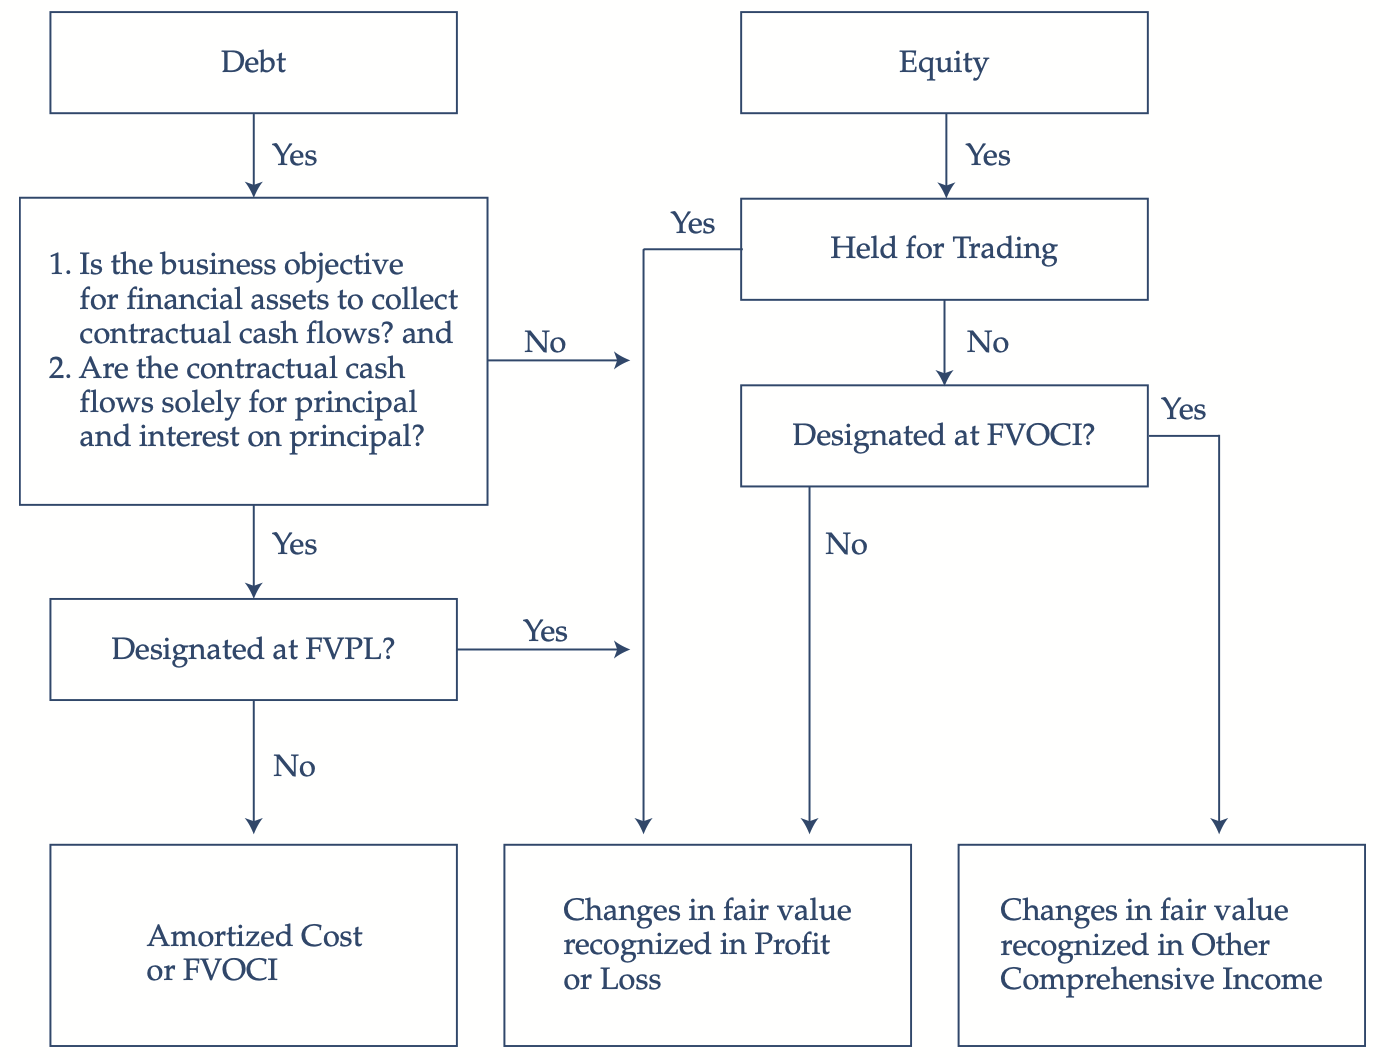
\includegraphics[scale=0.6]{fsa/ifrs9}
\caption{Financial Assets Classification and Measurement Model, IFRS9}
\label{fig:IFRS9}
\end{figure}

\begin{definition} \hlt{Investment in Financial Assets: IFRS 9}\\
IFRS 9 considers contractual characteristics of cash flow and management of financial assets.\\
For loan impairment, expected credit loss model will be used.
\end{definition}

\begin{method} \hlt{Amortised Cost Method - Debt Only}\\
Debt securities meeting following two criteria are accounted for using the amortised cost method:
\begin{enumerate}[label=\roman*.]
\setlength{\itemsep}{0pt}
\item Business Model Test: debt securities are being held to collect contractual cash flows
\item Cash Flow Characteristics Test: the contractual cash flows are principal, or interest on principal, only.
\end{enumerate}
These are reported on the balance sheet at amortised cost - the original cost of debt plus or minus any discount or premium that has been amortised to date.\\
Interest income (coupon cash flow adjusted for amortisation of premium or discount) is recognised in income statement; subsequent changes in fair value are ignored.
\end{method}

\begin{method} \hlt{Fair Value through Profit or Loss - Debt and Equity}
\begin{enumerate}[label=\roman*.]
\setlength{\itemsep}{0pt}
\item Debt: classified as FVPL if held for trading, or if accounting for these securities at amortised cost results in accounting mismatch (inconsistency from different measurement bases for assets and liabilities)
\item Equity: classified as FVPL if held for trading. Otherwise, may be classified as either FVPL or FVOCI, choice is irrevocable.
\item Derivatives: classified as FVPL if not used for hedging. If asset has embedded derivative (i.e., convertible bonds), asset as a whole is valued at FVPL.
\end{enumerate}
Securities are reported on balance sheet at fair value. Changes in fair value (realised and unrealised) are recognised in income statement with any dividend or interest income.
\end{method}

\begin{method} \hlt{Fair Value through Other Comprehensive Income - Debt and Equity}\\
Securities are reported on balance sheet at fair value; any unrealised gain or loss is reported on OCI.\\
Realised gains or losses, dividends, interest income are reported on the income statement.
\end{method}

\begin{flushleft}
\begin{tabularx}{\textwidth}{p{5em}|p{14.5em}|X|p{16em}}
\hline
\rowcolor{gray!30}
 & Amortised Cost & FVPL & FVOCI \\
\hline
Balance Sheet & Amortised cost & Fair Value & Fair value, with unrealised gains and losses (GL) recognised in equity \\
\hline
Income Statement & Interest (including amortisation) & Interest & Interest \\
& & Dividends & Dividends \\
& Realised GL & Realised GL & Realised GL \\
& & Unrealised GL & \\
\hline
\end{tabularx}
\end{flushleft}

\begin{method} \hlt{Reclassification under IFRS 9}
\begin{enumerate}[label=\roman*.]
\setlength{\itemsep}{0pt}
\item Debt: permitted only if business model has changed such that it significantly affects operations.
\item Equity: not permitted, as initial designation is irrevocable.
\end{enumerate}
\end{method}

\begin{method} \hlt{Loan Impairment under IFRS 9}\\
Incurred loss model for loan impairment replaced by expected credit loss model. Require companies to evaluate current and historical information on loan performance (loan commitments and lease receivables), and also forward-looking information.\\
Results in earlier recognition of loan impairment (12 month expected losses for performing loans, lifetime expected losses for non-performing loans).
\end{method}

\subsubsection{Investment in Associates: Equity Method}

\begin{remark} \hlt{Signs of Significant Influence}
\begin{enumerate}[label=\roman*.]
\setlength{\itemsep}{0pt}
\item Investment ownership between 20\% and 50\%
\item Representation on board of directors
\item Participation in the policy-making process
\item Material transactions between investor and investee
\item Interchange of managerial personnel
\item Technological dependency
\end{enumerate}
\end{remark}

\begin{method} \hlt{Equity Method}
\begin{enumerate}[label=\roman*.]
\setlength{\itemsep}{0pt}
\item Initial investment recorded at cost as non-current asset on BS.
\item Carrying amount of investment adjusted to recognise proportionate share of Profit and Loss (PnL); the PnL are recorded on IS.
\item Dividends and other distributions from investee is return of capital, reduce carrying amount of investment on BS, but not reported in investor PnL on IS.
\item On investee loss, investor will receive proportionate share of the loss, reducing the investment account, lower earnings in investor IS.
\item If investment value reduced to zero, equity method is discontinued; further losses will not be recorded. If investee subsequently reports profits, equity method is resumed after investor’s share of profit exceed the share of losses not recognised during the suspension period.
\end{enumerate}
\end{method}

\begin{remark} \hlt{Fair Value Option}
\begin{enumerate}[label=\roman*.]
\setlength{\itemsep}{0pt}
\item GAAP: allows investments to be recorded at fair value.
\item IFRS: fair value option only available to VC, mutual funds, unit trusts, ILPs etc. 
\end{enumerate}
Decision to use fair value option is irrevocable; any changes in value (with dividends) are recorded in IS.\\
Investor investment account on BS do not reflect proportionate share of PnL, dividends or other distributions. Excess of cost over fair value of investee identifiable net assets is not amortised, nor is goodwill created.
\end{remark}

\begin{remark} \hlt{Excess of Purchase Price over Book Value Acquired}
\begin{enumerate}[label=\roman*.]
\setlength{\itemsep}{0pt}
\item At acquisition, the difference is first allocated to specific assets and liabilities (AnL) of assets using fair values, accounted in manner consistent with accounting treatment for the specific AnL to which it is assigned. Amounts allocated to AnL which are expensed or depreciated to be similarly treated. \\
Initially the BS records the cost in the investment account.
\item The difference is then amortised to proportionate share of investee PnL over economic lives of the assets (whose fair value exceeds book value).\\
On the BS, as the differences are amortised, the balance in investment account will converge to proportionate share of book value of net assets of the associate.\\
Investor record these adjustments by reducing carrying amount of investment on BS and reducing investee profit recognised on its IS.
\item The goodwill is reviewed for impairment on regular basis. This is included in carrying amount of the investment on the investor BS.
\end{enumerate}
\end{remark}

\begin{method} \hlt{Investor Balance Sheet Impact: Equity Method}
\begin{align}
\text{Purchase Price} - \text{\% share of net asset BV} &= \text{Excess of purchase price} \nonumber \\
\text{Excess of purchase price} - \text{\% share of (FV} -  \text{BV) of PPE} &= \text{Goodwill} \nonumber \\
\text{Investor \% share of investee net income} - \text{Depreciation of \% share of excess PPE} &= \text{Equity income} \nonumber \\
\text{Investment balance beginning} + \text{Equity income} - \text{\% share of dividends} &= \text{Investment balance end} \nonumber
\end{align}
\end{method}

\begin{method} \hlt{Investor Income Statement Impact: Equity Method}
\begin{align}
\text{Impact} = \text{Equity income} - \text{\% share of unrealised profit from downstream and upstream sale} \nonumber
\end{align}
\end{method}

\begin{remark} \hlt{Treatment of PPE Depreciation on Investor}
\begin{enumerate}[label=\roman*.]
\setlength{\itemsep}{0pt}
\item IFRS: PPE is to be carried at either historical cost or fair value (less accumulated depreciation)
\item GAAP: PPE is to be carried at historical cost (less accumulated depreciation) only
\end{enumerate}
\end{remark}

\begin{method} \hlt{Impairment of Investments}\\
IFRS and GAAP require periodic reviews for impairment. If fair value of investment is less than carrying value permanently, impairment loss is recognised.
\begin{enumerate}[label=\roman*.]
\setlength{\itemsep}{0pt}
\item IFRS: require objective evidence due to one or more loss events that occur after initial recognition, and the loss event has impact on future CF reliably estimated.\\
Entire carrying amount tested by comparing recoverable amount with carrying amount.\\
Impairment loss recognised on IS; carrying amount on BS reduced directly or through allowance account.\\
Reversal of impairment loss allowed to extent that recoverable amount of net investment increases.
\item GAAP: treat impairment as permanent.\\
Impairment loss recognised on IS; carrying value of investment on BS reduced to fair value.\\
Prohibit reversal of impairment loss even if fair value later increases.
\end{enumerate}
\end{method}

\begin{remark} \hlt{Transactions with Associates}\\
Investor can influence terms and timing of transactions with associates. Profits from such transactions cannot be realised until confirmed through use or sale to third parties.\\
Investor share of unrealised profit deferred by reducing amount recorded under equity method. When deferred profit is confirmed, added this to equity income based on recorded values in associate’s accounts.
\begin{enumerate}[label=\roman*.]
\setlength{\itemsep}{0pt}
\item Upstream (investee to investor): profit recorded on investee IS as PnL. Investor’s share of unrealised profit is thus included in equity income on investor IS.\\
However, for profit that is unconfirmed (goods not been used or sold by investor), investor must eliminate proportionate share of profit from equity income of investee.
\item Downstream (investor to investee): profit recorded on investor IS. Investor must eliminate proportionate share of profit that is unconfirmed. Adjust equity income on investor’s IS by deducting on share percent.
\end{enumerate}
\end{remark}

\begin{remark} \hlt{Disclosures from Transactions with Associates}\\
Investee results are included in investor’s accounts with time lag (not more than one quarter). Dividends from investee are not included in investor income.\\
In consolidated BS, book value of shareholdings in investee is increased by investor’s share of associate net income, reduced by amortisation of surplus values and amount of dividends received.
\end{remark}

\begin{remark} \hlt{Analytical Issues of Equity Method}
\begin{enumerate}[label=\roman*.]
\setlength{\itemsep}{0pt}
\item Degree of control of investor on investee may not be proportional to shareholdings.
\item Significant AnL of investee are not reflected on investor BS, which affect debt ratios. Net margin ratios may be overstated as income for investee is included in investor net income, but not in sales.
\end{enumerate}
When analysing associates, consider quality of equity method earnings, potential restriction on dividend CF.
\end{remark}

\subsubsection{Business Combinations: Consolidation}

\begin{definition} \hlt{Types of Business Combinations}
\begin{enumerate}[label=\roman*.]
\setlength{\itemsep}{0pt}
\item \hlt{Merger}: Target 100\% absorbed. Net assets of Company B transferred to Company B.
\begin{equation}
\text{Company } A + \text{Company } B = \text{Company } A \nonumber
\end{equation}
\item \hlt{Acquisition}: Companies connected by parent-subsidiary relationship. May acquire less than 50\% and still exert control. May acquire less than 100\%, and non-controlling (minority) shareholder interest reported on consolidated financial statements.
\begin{equation}
\text{Company } A + \text{Company } B = (\text{Company } A + \text{Company } B) \nonumber
\end{equation}
\item \hlt{Consolidation}: New legal entity formed, take over net assets of both companies. 
\begin{equation}
\text{Company } A + \text{Company } B = \text{Company } C \nonumber
\end{equation}
\end{enumerate}
IFRS: no distinction made among business combinations.\\
GAAP: classified as merger, acquisition, or consolidation.
\end{definition}

\begin{method} \hlt{Pooling-of-Interests Method (IFRS Defunct)}\\
Ownership interest of two firms combined, participants viewed as equals.
\begin{enumerate}[label=\roman*.]
\setlength{\itemsep}{0pt}
\item Two firms asset and liabilities combined using historical book values
\item Operating results for prior periods restated as though the two firms were always combined
\item Ownership interests continue, former accounting bases are maintained
\end{enumerate}
\end{method}

\begin{method} \hlt{Acquisition Method: Recognition and Measurement}\\
Fair value of target includes acquisition-date fair value of any contingent consideration. Direct costs of business combination are expensed. Recognition and measurement of:
\begin{enumerate}[label=\roman*.]
\setlength{\itemsep}{0pt}
\item Identifiable assets and liabilities: measure at fair value at date of acquisition, including intangible assets
\item Contingent liabilities (CL): measure if it is a present obligation from past events, can be measured reliably.
\begin{enumerate}[label=\arabic*.]
\setlength{\itemsep}{0pt}
\item IFRS: includes CL if fair values can be reliably measured.
\item GAAP: only includes CL that are probable and can be reasonably measured.
\end{enumerate}
\item Indemnification assets (IA): recognise IA if seller contractually indemnifies acquirer for outcome of a contingency or uncertainty related to all or part of a specific asset or liability of the seller. Seller may also indemnify acquirer against losses above a specified amount on a liability arising from a particular contingency. Acquirer will recognise the IA at the acquisition date fair value.
\item Financial assets and liabilities: identifiable AnL are classified according to IFRS and GAAP standards. Acquirer reclassifies financial AnL based on contractual terms, economic conditions, acquirer’s operation and accounting policies.
\item Goodwill: GAAP requires full goodwill. IFRS prefers partial goodwill; full can be used. IFRS allows recognition on transaction-by-transaction basis. 
\begin{enumerate}[label=\arabic*.]
\setlength{\itemsep}{0pt}
\item Partial Goodwill: acquisition price less acquirer’s share of fair value of all tangible and intangible AnL, CL acquired. \begin{align}
\text{Partial Goodwill} &= \text{Acquisition Price} - \text{\% share of fair value of net identifiable assets} \nonumber \\
\text{Partial Goodwill} &= \text{Acquirer \% share of equity} \times \text{Full Goodwill} \nonumber \\
\text{Non-Controlling Interest} &= \text{\% share of NCI} \times \text{Acquiree fair value of identifiable net assets} \nonumber
\end{align}
\item Full Goodwill: fair value of entity less fair value of all tangible and intangible AnL, CL 
\begin{align}
\text{Full Goodwill} &= \text{Fair value of combined entity} - \text{fair value of net identifiable assets} \nonumber \\
\text{Non-Controlling Interest} &= \text{\% share of NCI} \times \text{Fair value of entity} \nonumber
\end{align}
\end{enumerate}
\item Bargain purchase: when acquisition price is less than fair value. Difference to be recognised immediately in PnL on IS. Any contingent consideration is measured and recognised at fair value; subsequent changes in value are recognised in PnL.
\end{enumerate}
\end{method}

\begin{remark} \hlt{Full Goodwill vs Partial Goodwill} \\
Full goodwill results in higher total assets and higher total equity than partial goodwill.\\
ROA and ROE will be lower if full goodwill method is used.
\end{remark}

\begin{method} \hlt{Investor Balance Sheet Impact: Acquisition Method}
\begin{align}
\text{End current assets} &= \text{Beginning current assets} + \text{acquiree current assets} - \text{acquisition cash fee} \nonumber \\
\text{End current liabilities} &= \text{Beginning current liabilities} + \text{acquiree current liabilities} \nonumber \\
\text{Minority Interest in Equity} &= \text{\% share of NCI} \times \text{Subsidiary equity} \nonumber
\end{align}
\end{method}

\begin{method} \hlt{Investor Income Statement Impact: Acquisition Method}
\begin{align}
\text{End revenue} &= \text{Beginning revenue} + \text{acquiree revenue} \nonumber \\
\text{End expenses} &= \text{Beginning expenses} + \text{acquiree expenses} \nonumber \\
\text{Minority Interest} &= - \text{\% share of NCI} \times \text{acquiree net income} \nonumber
\end{align}
Acquisition method results in higher revenue and expenses, but net income is the same.
\end{method}

\begin{method} \hlt{Goodwill Impairment}
\begin{enumerate}[label=\roman*.]
\setlength{\itemsep}{0pt}
\item IFRS: At acquisition, total goodwill recognised is allocated to each of acquirer’s cash generating units (lowest level within combined entity monitored for impairment purposes) that will benefit from expected synergies due to the combination with the target.\\
Impairment testing under one-step approach: If recoverable amount < carrying value of cash-generating unit, then impairment loss is recognised. 
\begin{equation}
\text{Impairment Loss} = \text{Carrying value of unit} - \text{Recoverable amount of unit} \nonumber
\end{equation}
Impairment loss is first applied to goodwill allocated to cash-generating unit; if reduced to zero, remaining amount allocated to other non-cash assets in the unit on pro-rata basis.
\item GAAP: At acquisition, total goodwill allocated to each of acquirer’s reporting units (operating segment or component of operating segment that is one level below operating segment as a whole).\\
Impairment testing under two-step approach: 
\begin{enumerate}[label=\arabic*.]
\setlength{\itemsep}{0pt}
\item If fair value < carrying value of reporting unit (with goodwill), potential impairment identified.
\begin{equation}
\text{Implied goodwill} = \text{Fair value of unit} - \text{Fair value of unit identifiable net assets} \nonumber
\end{equation}
\item Impairment loss is difference between carrying value of goodwill and implied fair value of goodwill.
\begin{equation}
\text{Impairment loss} = \text{Carrying value of goodwill} - \text{Implied goodwill} \nonumber
\end{equation}
\end{enumerate}
Impairment loss then applied to goodwill allocated to reporting unit; if reduced to zero, no other adjustment made to carrying value of any of reporting unit’s other AnL. Prudent to test other asset values for recoverability and possible impairment.
\end{enumerate}
IFRS and GAAP: impairment loss is recorded as separate line item in IS.
\end{method}

\subsubsection{Joint Ventures: Equity Method, Consolidation Method}

\begin{remark} \hlt{Purpose of Joint Ventures (JV)}\\
For entering foreign markets, conduct specialised activities, engage in risky projects.\\
May be primarily contractual relationships or common ownership of assets.\\
Can be partnerships, LLCs (corps) or other legal forms (unincorporated associations).\\
IFRS identify the characteristic of JVs as follows: a contractual agreement exists between two or more venturers, and the contract establishes joint control.
\end{remark}

\begin{method} \hlt{Equity Method vs Consolidation Method}
\begin{enumerate}[label=\roman*.]
\setlength{\itemsep}{0pt}
\item Proportional consolidation: require venturer’s share of assets, liabilities, income, expenses of JV to be combined or show on line-by-line basis with similar items under its sole control.
\item Equity method: line item 'equity in income of JV' on IS, line item 'investment in JV' on BS.
\end{enumerate}
Proportionate consolidation results in higher AnL, but stockholder's equity and net assets is the same. Proportionate consolidation also results in higher revenues and expenses, but net income is the same.
\end{method}

\subsubsection{Special Purpose Entities, Variable Interest Entities}

\begin{remark} \hlt{Purpose of Special Purpose Entities (SPEs)}\\
Sponsor transfers assets to SPE, obtains right to use assets held by SPE, or perform services for the SPEs. Third party provide funding to the SPE.\\
Third party interest may take form of debt, equity, participation right, or residual interest in a lease. Sponsor retains significant beneficial interest, even if it may own little or none of SPE’s voting equity.\\
For segregation of certain activities, hence reduce risk and lower cost of financing.\\
Typically structured such that sponsor has control over SPE finances or operating activities, and third parties have controlling interest in SPE equity.
\end{remark}

\begin{remark} \hlt{IFRS Sponsor Control of SPEs}\\
IFRS require consolidation if there is sponsor control, where:
\begin{enumerate}[label=\roman*.]
\setlength{\itemsep}{0pt}
\item Investor has ability to exert influence on financial and operating policy of entity.
\item Investor is exposed, or has rights to variable returns from involvement with entity.
\end{enumerate}
SPEs involved in structured financial transaction will require evaluation of the purpose, design and risks.
\end{remark}

\begin{definition} \hlt{Primary Beneficiary}\\
The party that will absorb the majority of SPE expected losses, receive the majority of SPE expected residual returns, or both.
\end{definition}

\begin{remark} \hlt{GAAP Classification of SPE as VIE}\\
VIE includes other entities besides SPEs. Classifies SPE as VIE if one of the conditions is met:
\begin{enumerate}[label=\roman*.]
\setlength{\itemsep}{0pt}
\item Total equity at risk insufficient to finance activities without financial support from other parties; or
\item Equity investors lack one of the following: 
\begin{enumerate}[label=\arabic*.]
\setlength{\itemsep}{0pt}
\item Ability to make decisions
\item Obligation to absorb losses
\item Right to receive returns
\end{enumerate}
\end{enumerate}
\end{remark}

\begin{method} \hlt{GAAP Consolidation for SPEs and VIEs}
\begin{enumerate}[label=\roman*.]
\setlength{\itemsep}{0pt}
\item SPEs: Require primarily beneficiary to consolidate the SPE regardless of its voting interest in the SPE, or its decision-making authority.\\
Two-component consolidation: variable interest component and voting interest (control) component.
\item VIEs: Primary beneficiary of VIE must consolidate it as subsidiary regardless of how much equity the beneficiary has in VIE. The entity absorbing majority of losses must consolidate the VIE if another entity receive majority of VIE’s expected residual returns. Entities must disclose relationship with VIE even if not the primary beneficiary.\\
Non-controlling interests in the VIE must be shown on the consolidated BS and IS of primary beneficiary. 
\end{enumerate}
\end{method}

\subsubsection{Issues that Impair Comparability}

\begin{remark} \hlt{Contingent Assets and Liabilities}
\begin{enumerate}[label=\roman*.]
\setlength{\itemsep}{0pt}
\item IFRS: contingent assets are never recognised.\\
Contingent liabilities whose fair value can be measured reliably are recognised at time of acquisition. Subsequently, contingent liabilities measured at the higher of value initially recognised or best estimate of amount needed to settle.
\item GAAP: Contractual contingent AnL recorded at fair value at date of acquisition. Non-contractual contingent AnL also recorded if 'more likely than not' they meet the definition of an asset or liability.\\
Subsequently, contingent liabilities are measured at higher of amount initially recognised, or best estimate of amount of the loss. Contingent assets are measured at lower of acquisition date fair value or best estimate of the future settlement amount.
\end{enumerate}
\end{remark}

\begin{remark} \hlt{Contingent Consideration}\\
If terms of acquisition involve contingent consideration, this is recognised at fair value under both IFRS and GAAP as an asset, liability, or equity.\\
Subsequent changes in fair value are recognised in income statement, unless value was originally classified in equity (any changes settle within equity and not on IS).
\end{remark}

\begin{remark} \hlt{In-Process R\&D}\\
In-Process R\&D is capitalised as separate intangible asset, measured at fair value (if can be measured reliably).\\
In subsequent periods, this is subject to amortisation if fully completed, or impairment if no product results or if product is not technically and/or financially viable.
\end{remark}

\begin{remark} \hlt{Restructuring Costs}\\
IFRS and GAAP do not recognise restructuring costs. This is recognised as an expense in the periods the restructuring costs are incurred.
\end{remark}

\begin{remark} \hlt{Choice of Accounting Method on BS and IS Items}
\begin{enumerate}[label=\roman*.]
\setlength{\itemsep}{0pt}
\item Net Income: same for all three methods
\item Equity: Equity method and proportionate consolidate has same equity. Acquisition method equity will be higher by amount of minority interest.
\item Assets and Liabilities: highest under acquisition method, lowest under equity method.
\item Revenues and Expenses: highest under acquisition method, lowest under equity method.
\end{enumerate}
\end{remark}

\begin{flushleft}
\begin{tabularx}{\textwidth}{p{8em}|p{17.5em}|p{10em}|X}
\hline
\rowcolor{gray!30}
 & Equity & Prop Cosol & Acquisition \\
\hline
Net Profit Margin & Higher (sales lower, net income same) & In-Between & Lower \\
\hline
ROE & Higher (equity lower, net income same) & Same as equity method & Lower \\
\hline
ROA & Higher (net income same, assets lower) & In-Between & Lower \\
\hline
\end{tabularx}
\end{flushleft}

\newpage




\newpage

\section{Corporate Issuers}

\subsection{Analysis of Dividends and Share Repurchases}

\begin{definition} Common Terminology
\begin{enumerate}[label=\roman*.]
\setlength{\itemsep}{0pt}
\item \hlt{Ex-Dividend Date}: first date that shares trade without right to receive declared dividend for the period.
\item \hlt{Payout Policy}: set of principles guiding cash dividends and value of shares repurchased
\end{enumerate}
\end{definition}

\begin{remark} Types of Dividends
\begin{enumerate}[label=\roman*.]
\setlength{\itemsep}{0pt}
\item \hlt{Regular Cash Dividends}: distribution of cash. Firms strive for stability by increasing them slowly, refraining from any reductions. Stable or increasing dividends are signs of consistent or increasing profitability.\\
Frequency of payment vary. US and Canadian companies typically pay quarter, European and Asian companies typically pay semiannually and annually.
\item \hlt{Extra or Special (Irregular) Dividends}: cash dividend supplementing regular dividends, or dividend from company that normally does not pay dividends. Paid under special circumstances with expectation that dividend is not recurring, or when company has a very profitable year but does not want to commit to higher ongoing regular dividend payment. Usually used by firms in cyclical industries.
\item \hlt{Liquidating Dividend}: paid when the company:
\begin{enumerate}[label=\arabic*.]
\setlength{\itemsep}{0pt}
\item is bankrupt, and net assets (after all liabilities are paid) are distributed to shareholders
\item sells a portion of its business for cash, proceeds distributed to shareholders
\item pays a dividend that exceeds accumulated retained earnings (reduces stated capital)
\end{enumerate}
Liquidating dividend is a return of capital, rather than a return on capital.
\item \hlt{Stock Dividend}: non-cash dividend paid in form of additional shares. After payment, shareholders have more shares, and cost per shares will be lower. Shareholder proportionate ownership does not change, as each shareholder receives same percentage of stock dividend. Stock dividends are not taxed. Market price per share declines, leaving shareholders with no net gain.\\
Stock dividends encourage long-term investing, hence may reduce cost of equity capital. Stock dividends also increase stock float and hence its liquidity, and decrease market price of stock to a desirable trading range that attracts more investors.\\
Companies paying same regular cash dividend per share has increased their share dividend, but companies that have the same payout ratio would decrease dividend per share (dividend yield unchanged).\\
Stock dividend is accounted for as transfer of retained earnings to contributed capital.
\item \hlt{Stock Splits}: similar to stock dividends but larger in size. Reverse stock splits reduce number of shares outstanding and increase price per share, used to increase market price of stock to a desirable range to attract institutional investors and mutual funds that shun low-priced stocks.
\end{enumerate}
\end{remark}

\begin{remark} \hlt{Effects of Dividends on Financial Statement and Ratios}\\
Cash dividend payments reduce cash and stockholders equity, resulting in lower quick ratio and current ratio, and higher leverage ratios (i.e., debt-to=equity, debt-to-asset).\\
Stock dividends, stock splits or reverse stock splits leave the capital structure unchanged, do not affect ratios.\\
For stock dividend, decrease in retained earnings (corresponding to value of stock dividend) is offset by increase in contributed capital, leaving value of total equity unchanged.\\
Stock split or reverse stock split does not affect book value of equity and tax cost basis for shareholders.
\end{remark}

\subsubsection{Theory of Dividend Policy}

\begin{remark} \hlt{Dividend Irrelevance Theory}\\
Based on Miller and Modigliani (MM), under perfect capital market assumptions (no taxes, transaction costs, equal information), dividend policy should have no impact on cost of capital or shareholder wealth. The MM theory is based on the firm's total payout policy.\\
Theory is based on concept of 'homemade dividends', where an investor may tailor his own dividends irrespective of company dividend policy. If cash dividend is too large, investor may take excess cash received and buy more stock. If cash dividend is too small, investor may sell some stock to get the cash flow. Hence, combination of value of investor investment in firm and cash in hand will be the same.\\
In real world, market imperfections causes issues, as companies issuing new shares incurs flotation costs. Shareholders selling shares would incur transaction costs and capital gain taxes.  Selling shares on periodic basis will be problematic if share prices are volatile.
\end{remark}

\begin{remark} \hlt{Dividend Preference Theory (Bird in Hand Argument)}\\
Even under perfect capital market assumptions, investors prefer dollar of dividends to dollar of potential capital gains from earnings as dividends are viewed as less risky.\\
Company that pays dividends will have lower cost of equity capital than a company that does not pay dividends, hence this should result in a higher share price.\\
When measuring total return, dividend yield component $\frac{D_1}{P_0}$ is less risky than growth component $g$.
\end{remark}

\begin{remark} \hlt{Tax Aversion Theory}\\
Investors prefer not to receive dividends due to higher tax rates. In the extreme, this implies investors would ant companies to have zero dividend payout ratio.\\
In real world, tax laws prevent companies from accumulating excess earnings; dividend payments necessary.
\end{remark}

\begin{remark} \hlt{Information Asymmetry}\\
Company board and management have more information compared to investors. Dividends convey credit information to investors, as dividends entail actual cash flow and are expected to continue in the future.\\
Companies avoid increasing dividends unless higher levels of dividends are expected to continue in the future. Dividends will not decrease unless companies expect long-run poorer prospects of the company in the future.
\end{remark}

\begin{remark} \hlt{Dividend Initiation}\\
Information conveyed is ambiguous. Dividend initiation may indicate that company is optimistic about its future and is sharing its wealth with stockholders; company may also have lack of profitable investment opportunities.
\end{remark}

\begin{remark} \hlt{Unexpected Dividend Increase}\\
Signal that business prospects are strong, managers will share success with shareholders.\\
Companies with long history of dividend increases are dominant in their industries, and have high return on assets and low debt ratios.
\end{remark}

\begin{remark} \hlt{Unexpected Dividend Decrease or Omissions}\\
Typically negative signals that business is in trouble, management does not believe current dividend payment can be maintained. May also mean profitable investment opportunities are available, shareholders will receive greater benefit by having earnings reinvested in company.
\end{remark}

\begin{remark} \hlt{Agency Costs and Dividends as Control Mechanism}
\begin{enumerate}[label=\roman*.]
\setlength{\itemsep}{0pt}
\item Between shareholders and managers: managers have incentive to over-invest, leading to investment in some negative NPV projects which reduces stockholder wealth. To reduce agency cost, increase payout of FCF as dividends. Mature firms in relatively non-cyclical industries do not need to hoard cash, hence a higher dividend payout would be welcomed by investors, resulting in increases in stock value.
\item Between shareholders and bondholders: when there is risky debt outstanding, shareholders may pay themselves a large dividend, leaving bondholders with lower asset base as collateral, hence resulting in wealth transfer from bondholders to stockholders. Typically resolved via provisions in bond indentures, which include restrictions on dividend payment, maintenance of certain BS ratios, etc.
\end{enumerate}
\end{remark}

\begin{definition} \hlt{Taxation Methods}
\begin{enumerate}[label=\roman*.]
\setlength{\itemsep}{0pt}
\item Double taxation system: corporate pretax earnings taxed at corporate levels, then taxed again at shareholder level if distributed to taxable shareholders as dividends.
\item Dividend imputation tax system: corporate earnings first taxed at corporate level. When earnings are distributed to shareholders as dividends, shareholders receive a tax credit (franking credit). If shareholder's marginal tax rate is higher than company's, shareholder pays the difference between the two rates.
\end{enumerate}
\end{definition}

\begin{remark} \hlt{Factors Affecting Dividend Payout Policy}
\begin{enumerate}[label=\roman*.]
\setlength{\itemsep}{0pt}
\item Investment opportunities: availability of positive NPV investment opportunities and speed at which firm must react to opportunities determine amount of cash firm must keep at hand. If there are many profitable opportunities and quick reaction required, dividend payout must be low.
\item Expected volatility of future earnings: firms tie target payout ratio to long-run sustainable earnings, are reluctant to increase dividends unless reversal is not expected in the near future.\\
When earnings are volatile, firms are more cautions in changing dividend payout.
\item Financial flexibility: firms with excess cash and desire to maintain financial flexibility may use stock repurchases instead of cash dividends, which is less sticky. Having cash on hand allows flexibility to meet unforeseen operating needs and investment opportunities, which is especially important in times of crisis where liquidity is low and credit is hard to obtain.
\item Tax considerations: depends on method and amount of tax applied on dividend payment.\\
For companies with favourable capital gains tax compared to dividends, high-tax-bracket investors prefer low dividend payouts, low-tax-bracket investors prefer high dividend payouts.\\
Lower dividend tax rate compared to capital gains do not mean companies will raise their dividend payouts. Stockholders may not prefer higher dividend payout as:
\begin{enumerate}[label=\arabic*.]
\setlength{\itemsep}{0pt}
\item taxes on dividends are paid when dividend is received, while capital gains taxes are paid only when shares are sold
\item cost basis of shares may receive step-up in valuation at shareholder's death, hence taxes on capital gains may not have to be paid at all
\item tax-exempt institutions will be indifferent between dividends or capital gains
\end{enumerate}
\item Flotation costs: when company issues new shares of common stock, flotation costs of $3\%$ to $7\%$ is taken from amount of capital raised to pay for costs associated with issuing new stock. As retained earnings have no such fee, cost of new equity capital is always higher than cost of retained earnings.\\
Larger companies have lower flotation costs as compared to smaller companies.\\
The higher the flotation costs, the lower the dividend payout.
\item Contractual and legal restrictions: Companies may be restricted from paying dividends by legal requirements, or by implicit restrictions due to cash needs of the business:
\begin{enumerate}[label=\arabic*.]
\setlength{\itemsep}{0pt}
\item Impairment of capital rule: dividends paid cannot be in excess of retained earnings
\item Debt covenants; designed to protect bondholders. May have target for liquidity ratios and coverage ratios before a dividend can be paid
\end{enumerate}
\end{enumerate}
\end{remark}


\begin{definition} \hlt{Taxation Methods}
\begin{enumerate}[label=\roman*.]
\setlength{\itemsep}{0pt}
\item Double taxation system: corporate pretax earnings taxed at corporate levels, then taxed again at shareholder level if distributed to taxable shareholders as dividends.
\begin{equation}
\text{Effective tax rate} = \text{Corporate tax rate} + (1-\text{Corporate tax rate})(\text{Individual tax rate}) \nonumber
\end{equation}
\item Split rate tax system: earnings distributed as dividends are taxes at lower rate than earnings retained. Effect is to offset the higher (double) tax rate applied to dividends at individual level.\\
Calculation of effective rate is similar to that under double taxation, except rate applicable would be corporate tax rate for distributed income
\item Dividend imputation tax system: taxes paid at corporate level but are attributed to shareholder, hence all taxes are effectively paid at shareholder rate.\\
Shareholders deduct their portion of taxes paid by corporation from their tax return. If shareholder tax bracket is lower than company rate, shareholder receive tax credit (franking credit) equal to the difference. If shareholder tax bracket is higher than company rate, shareholder pays the difference.\\
Effective tax rate on dividend is simply the shareholder's marginal tax rate.
\end{enumerate}
\end{definition}

\subsubsection{Payout Policies and Share Repurchases}

\begin{method} \hlt{Target Payout Adjustment Model}\\
Model of gradual adjustment from stable dividend payout policy to target dividend payout ratio.\\
If company earnings are expected to increase, and current payout ratio is below target payout ratio, investor may estimate future dividends with the following:
\begin{align}
\text{Expected increase in dividends} &= [(\text{Expected earnings} \times \text{Target payout ratio}) - \text{Previous dividend}]\times \text{Adj Fac} \nonumber \\
\text{Adj Fac} &= \frac{1}{\text{Number of years which adjustment in dividends will take place}} \nonumber
\end{align}
\end{method}

\begin{remark} \hlt{Trends in Dividend Payout Policy}
\begin{enumerate}[label=\roman*.]
\setlength{\itemsep}{0pt}
\item In developed markets, proportion of companies paying cash dividends trend downwards over LT.
\item Percentage of companies making stock repurchases are trending upwards in US since 1980s and in UK and EU since 1990s. Major companies in Asia (CN, JP), made substantial repurchases since 2010s.
\end{enumerate}
\end{remark}

\begin{remark} Share Repurchase Methods
\begin{enumerate}[label=\roman*.]
\setlength{\itemsep}{0pt}
\item \hlt{Open Market Transactions}: most flexible, allow company to buyback shares at most favourable terms. No obligation for company to complete an announced buyback program.\\
US companies do not need shareholder approval for open market transactions, unlike EU companies.
\item \hlt{Fixed-Price Tender Offer}: firm buys a predetermined number of shares at a fixed price (typically premium over current market price). Company forgoes flexibility to buy back shares quickly.\\
If more than desired number of shares tendered to offer, company will buyback prorated number of shares from each shareholder responding to the offer.
\item \hlt{Dutch Auction}: tender offer where company specifies a range of prices. Identify minimum clearing price for desired number of shares that need to be repurchased. Each participating shareholder indicates price and number of shares tendered. Bids accepted based on lowest price first until desired quantity is filled. Price of last offer accepted will be price paid for all shares tendered. Can be accomplished quickly, but not as quick as tender offers.
\item \hlt{Repurchase by Direct Negotiation}: purchase shares from a major shareholder with premium over market price. Used in greenmail scenario (hostile bidder is offered a premium to go away), also to remove a large overhang in the market that is dampening the share price. Many negotiated transactions occur at discount to market price, indicating urgent liquidity needs of the seller motivating the transaction.
\end{enumerate}
\end{remark}

\begin{remark} \hlt{Financial statement Effects of Repurchases}\\
Repurchases made with surplus cash will decrease cash and shareholder's equity, hence increasing leverage.\\
After repurchase, earnings per share may increase, depending on how much cash was used.\\
If repurchase was financed with additional debt offerings, reduction in net income from (after-tax) cost of borrowed funds to be factored to determine impact on earnings per share.\\
If price paid for share repurchase is higher (lower) than pre-repurchase book value per share (BVPS), then BVPS will decrease (increase).\\
If cost of capital is greater than earnings yield (earnings-to-price ratio), then earnings dilution will result from buyback. If earnings yield is greater than after-tax cost of borrowed funds, EPS will increase.
\end{remark}

\begin{remark} \hlt{Rationales for Share Repurchases}
\begin{enumerate}[label=\roman*.]
\setlength{\itemsep}{0pt}
\item Potential tax advantages: If tax rate on capital gains is lower than tax rate on dividend income, share repurchases have tax advantage over cash dividends.
\item Share price support/signalling: share repurchase signals to market that company views its own stock as a good investment and the future outlook is good, and is important in presence of asymmetric information. Tactic is often used when share price is declining, and management wants to convey confidence.
\item Added flexibility: as paying cash dividend and repurchasing shares are economically equivalent, company could declare small stable dividend, then repurchase shares with leftover earnings. Managers have discretion with respect to market timing of their repurchases.
\item Offsetting dilution from employee stock options: offset EPS dilution from exercise of employee options.
\item Increasing financial leverage: if funded by new debt. May change company's capital structure towards a more optimal one by decreasing the percentage of equity.
\end{enumerate}
\end{remark}

\begin{remark} \hlt{Dividend Safety}\\
Metric used to evaluate probability of dividends continuing at the current rate for a company.\\
Traditional ratios such as dividend payout ratio, or its inverse (dividend coverage ratio) are typically used for this purpose. A higher than normal payout ratio indicates a higher probability of dividend cut.\\
Compare the computed ratio to average ratio for the industry and market within which a company operates. Stable or increasing dividends are more favourable.\\
FCFE Coverage Ratio may also be considered, where dividends and share repurchases are both considered:
\begin{equation}
\text{FCFE Coverage Ratio} = \frac{\text{FCFE}}{\text{Dividends} + \text{Share repurchases}} \nonumber
\end{equation}
FCFE coverage ratio significantly less than one is considered unsustainable, as company is drawing down its cash reserves for dividends and repurchases.
\end{remark}

\newpage

\subsection{ESG Considerations in Investment Analysis}



\newpage

\subsection{Cost of Capital}

Recall that the weight average cost of capital (WACC) is as follows:
\begin{equation}
\text{WACC} = w_e r_e + w_p r_r + w_d r_d (1-t) \nonumber 
\end{equation}
where $r_e$ is cost of equity, $r_p$ cost of preferred equity, $r_d$ cost of debt, and $w_e, w_r, w_d$ cost of weights. Consider the after-tax cost of debt if interest expense is tax-deductible, using the marginal tax rate.

\subsubsection{Cost of Capital Factors}

\begin{remark} Top-down factors that impact cost of capital are as follows:
\begin{enumerate}[label=\roman*.]
\setlength{\itemsep}{0pt}
\item \hlt{Capital Availability}: if economy has greater availability of capital, the cost will be lower. Developed economies with established, liquid capital markets, more stable currencies, better protection and law will have lower cost of capital. In some less-developed markets with lack of corporate debt markets, companies rely on other means for funding, such as bank loans or shadow banking system.
\item \hlt{Market Conditions}: lower expected inflation lead to lower nominal risk-free rates. Risk premiums on debt and equity decrease during economic expansions, and increase during economic contractions. Transparent and predictable monetary policies lead to lower risk premiums and interest rates. Higher currency volatility leads to higher risk premiums for risk-averse investors.
\item \hlt{Legal and Regulatory Considerations, Country Risk}: countries that follow common law-based legal systems have stronger legal systems, hence lower risk premiums compared to that of civil law-based legal systems.
\item \hlt{Tax Jurisdiction}: the higher the marginal tax rate, the greater the tax benefit of using debt.
\end{enumerate}
\end{remark}

\begin{remark} Bottom-up factors that impact cost of capital are as follows:
\begin{enumerate}[label=\roman*.]
\setlength{\itemsep}{0pt}
\item \hlt{Business or Operating Risk}: business with stable revenues, earnings and cash flows are less risky. Companies with higher customer concentration risk require more risk premium. Companies with higher leverage has higher volatility of earnings and cash flows require higher risk premiums. Companies with poor corporate governance, higher ESG-risk exposures will require higher risk premiums.
\item \hlt{Asset Nature and Liquidity}: companies with higher proportion of tangible, fungible assets have higher recovery rate, hence lower risk premium. Specialised assets and intangibles do not have a ready liquid market, hence have lower recovery rate. Assets designated as collateral reduce cost of secured debt, but increase cost of other subordinated unsecured debt as their claim becomes superior.
\item \hlt{Financial Strength and Profitability}: companies with higher profitability, higher ability to generate cash, lower leverage, have lower probability of default, hence a lower risk premium. 
\item \hlt{Security Features}: embedded call options increases current cost of borrowing for issuer, and allows company to refinance the debt at a favourable rate should if interest rates decline. Converse is true for put option. Cumulative preferred stock accumulates missed dividends when company is unprofitable, hence has lower risk premium. Common equity with inferior rights have higher costs than that of superior rights.
\end{enumerate}
\end{remark}

\begin{flushleft}
\begin{tabularx}{\textwidth}{X|p{5em}|p{5em}}
\hline
\rowcolor{gray!30}
Revenues, Earnings, and Cash Flow Volatility & Lower & Higher \\
\hline
Higher stability of revenues, earnings, and cash flows & \checkmark & \\
Higher revenue concentration & & \checkmark \\
Higher earnings predictability & \checkmark & \\
Higher operating leverage & & \checkmark \\
Higher financial leverage & & \checkmark \\
Higher ESG risks & & \checkmark \\
\hline
\rowcolor{gray!30}
Asset Nature and Liquidity & Lower & Higher \\
\hline
Higher proportion of fungible, tangible assets & \checkmark & \\
Higher proportion of liquid assets & \checkmark & \\
\hline
\rowcolor{gray!30}
Financial Strength, Profitability, and Financial Leverage & Lower & Higher \\
\hline
Higher profitability & \checkmark & \\
Higher cash flow generation & \checkmark & \\
Higher interest coverage ratio, liquidity & \checkmark & \\
Higher leverage ratio & & \checkmark \\
\hline
\rowcolor{gray!30}
Security Features & Lower & Higher \\
\hline
Debt: call features & & \checkmark \\
Debt: put features & \checkmark & \\
Debt: conversion feature & \checkmark & \\
Preferred Equity: cumulative feature & \checkmark & \\
Common Equity: inferior cash flow or voting rights & & \checkmark \\
\hline
\end{tabularx}
\end{flushleft}

\subsubsection{Cost of Debt Estimation}

\begin{method} \hlt{Traded Debt}\\
If corporate debt is publicly traded, the yield to maturity (YTM) for longest maturity straight debt (debt with no embedded options) is the best estimate of cost of debt. If there exists shorter-term bonds that are more liquid than longest dated bond, YTM for this may be used instead.	
\end{method}

\begin{method} \hlt{Non-Traded Debt}\\
For private companies, or public companies with non-traded or illiquid debt securities.\\
If credit rating exists, estimate YTM with matrix pricing by considering bonds of other companies with same or similar maturities and credit ratings. If credit rating does not exist, use interest coverage ratio or financial leverage ratio to deduce credit rating.\\
Alternatively, credit spread of specific credit rating and maturity may be applied to benchmark rates.\\
Note, a company may have different ratings depending on debt collateral, seniority, convertibility, and other features. Hence, issuer rating may differ from issuer's individual series of debt.
\end{method}

\begin{method} \hlt{Bank Debt}\\
Determine interest on new bank debt financing for company to estimate cost of bank debt; if new bank debt is recent, then this may be good estimate of cost of debt if interest rate reflects current market conditions, and company risk profile has not changed materially since issuance.
\end{method}

\begin{method} \hlt{Leases}\\
A finance or capital lease is an example of amortised loan, and can be used to estimate cost of borrowing. The rate implicit in the least (RIIL) is the implied cost of capital, which is IRR from:
\begin{equation}
\text{PV of lease payments} + \text{PV of residual value} = \text{Fair value of leased asset} + \text{Lessor's direct initial cost} \nonumber
\end{equation}
If present value of residual value and lessor's direct initial costs are unknown, the incremental borrowing rate (IBR) (rate on new secured loan over same term) may be used.
\end{method}

\begin{method} \hlt{International Considerations for Cost of Debt Estimation}\\
For foreign market, country risk premium is added to debt's yield.\\
A country risk rating (CRR) may be used, which reflects risk related to economic conditions, political risk, exchange rate risk, securities market development and regulation. Country may be assigned a rating relative to benchmark country, which excess of the median interest rate relative to benchmark is the CRR.
\end{method}

\subsubsection{Cost of Equity Estimation}

\begin{method} \hlt{Equity Risk Premium (ERP) Historical Estimates}\\
Approach used when reliable long-term equity return data is available. Typically calculated as mean value of difference between broad-based equity index return and a government debt return (as proxy for risk-free rate).\\
Returns are assumed to be stationary, markets relatively efficient. Decisions to make includes:
\begin{enumerate}[label=\roman*.]
\setlength{\itemsep}{0pt}
\item Equity Index Selection: select an index that accurately represents typical returns earned by equity investors. Broad-based, market-value-weighted indexes typically chosen.
\item Time Period: longer time period that covers multiple business cycles and variety of market conditions should be covered. Older data may not reflect current market conditions,
\item Selection of Mean Type: arithmetic mean is easy to calculate, but is sensitive to extreme values, and overestimated the expected terminal value of wealth. Geometric mean gives outliers less weight, and estimates the expected terminal value of wealth more accurately, hence is more preferred.
\item Selection of Risk-Free Rate Proxy: as duration of equity is long-term (infinite), long-term government bond rates is preferred as proxies for risk-free rate\\
\begin{tabularx}{\textwidth}{p{12.5em}|X|X}
\hline
\rowcolor{gray!30}
Risk-Free Proxy & Advantages & Disadvantages \\
\hline
Short-Term Govt Bill Rate & Exact estimate of risk-free rate, assuming no default & does not closely match duration of infinite-life equity security \\
\hline
Long-Term Govt Bond YTM & YTM more closely match duration of infinite-life equity security & YTM not completely risk-free (unknown coupon reinvestment rates) \\
\hline
\end{tabularx}
\end{enumerate}
\end{method}

\begin{remark} \hlt{Limitations of Historical Approach for Computing ERP}
\begin{enumerate}[label=\roman*.]
\setlength{\itemsep}{0pt}
\item ERPs are countercyclical; low during economic expansion, high during contractions. Estimates based on long time series of historical data is not representative of future ERP.
\item Survivorship bias inflate historical estimates of ERP. Bias is in equity market data when poorly performing or defunct companies are removed from index membership.
\end{enumerate}
\end{remark}

\begin{method} \hlt{Equity Risk Premium (ERP) Forward-Looking Approach}\\
Approach uses current information and expectations on economic and financial variables. Do not rely on assumption of stationarity, and less affected by survivorship bias.
\end{method}

\begin{method} \hlt{Forward-Looking Approach: Survey-Based Estimates}\\
Uses consensus of opinions from experts. Surveys tend to higher ERPs for developing markets relative to developed markets. Biased toward recent market returns.
\end{method}

\begin{method} \hlt{Forward-Looking Approach: Dividend Discount Model Estimates}\\
Simplified model uses expected constant earnings growth rate (Gordon Growth Model), and solving for required return on equity yields
\begin{equation}
r_e = \frac{D_1}{V_0} + g \nonumber
\end{equation}
where $V_0$ is present value of future expected dividends, $\frac{D_1}{V_0}$ is expected dividend yield, $g$ is expected earnings growth rate. Broad-based equity indexes have associated dividend yield, and year-ahead dividend $D_1$ may be fairly predictable. Expected earnings growth rate $g$ may be inferred based on analyst expectations, which can be top-down or bottom-up generated forecasts.\\
Subtracting current risk-free rate from expected market equity return yields forward-looking ERP:
\begin{equation}
\text{ERP} = E\left[\frac{D_1}{V_0}\right] + E[g] - r_f \nonumber 
\end{equation}
Constant growth model assumes constant growth rate in earnings and dividends; else an adjustment on anticipated P/E multiple expansion or contraction needs to be done. P/E increase may be due to increase in earnings growth rate or decrease in risk (vice versa). \\
Aggregate amount spent on buybacks by index constituent companies may be included in dividend yield to reflect total payout; consider degree to which buyback alter growth rates in earnings and dividends.\\
For rapidly growing economies, a three stage growth model (fast, transition, mature) may be used. 
\begin{equation}
\text{Equity Index Price} = PV_{\text{Fast}} + PV_{\text{Transition}} + PV_{\text{Mature}} \nonumber
\end{equation}
The $IRR$ from this is then the required rate of return. Subtract current risk-free rate to get ERP.
\end{method}

\begin{method} \hlt{Forward-Looking Approach: Macroeconomic Model}\\
Grinold-Kroner model is used, which decomposes ERP as follows:
\begin{align}
\text{ERP} &= [\text{Dividend Yield} + \text{Capital Gains Yield}] - E[r_f] \nonumber \\
&= [\text{Dividend Yield} + \text{Expected Repricing} + \text{Earnings Growth per Share}] - E[r_f] \nonumber \\
&= \left[DY + \Delta (P/E) + i + g - \Delta S \right] - E[r_f] \nonumber
\end{align}
\begin{tabularx}{\textwidth}{p{14em}|p{4em}|X}
\hline
\rowcolor{gray!30}
Factor & Symbol & Common Proxy \\
\hline
Expected income component & DY & Broad-based market index dividend yield \\
\hline
Expected growth rate in P/E & $\Delta (P/E)$ & Adjust for market over or under valuation (commonly $0$) \\	
\hline
Expected inflation & $i$ & (nominal yield $-$ real yield) for similar maturity security \\
\hline
Expected growth in real EPS & $g$ & Real GDP growth \\
\hline
Expected $\Delta$\% in shares outstd & $\Delta S$ & Depends on market and time period \\
\hline
\end{tabularx}\\

Common approach to estimate expected inflation is to compare nominal yield on US Treasury bond to yield on equivalent inflation-protected Treasury security (TIPS):
\begin{equation}
i = \frac{1 + \text{YTM}_{\text{Treasury Bond}}}{1 + \text{YTM}_{\text{TIPS}}} - 1 \approx \text{YTM}_{\text{Treasury Bond}} - \text{YTM}_{\text{TIPS}} \nonumber
\end{equation}
\end{method}

\begin{remark} \hlt{Limitations of Forward-Looking Approach for Computing ERP}\\
\begin{tabularx}{\textwidth}{p{5em}|X}
\hline
\rowcolor{gray!30}
Factor & Symbol \\
\hline
Surveys & Subject to sampling and response biases, behavioural biases (recency bias, confirmation bias) \\
\hline
DDM & Assumes constant P/E. Adjustment on P/E to reflect multiple expansion or contraction \\
\hline
Macroecon & Models may have modelling errors or behavioural biases in forecasting \\
\hline
\end{tabularx}
\end{remark}

\begin{method} \hlt{ERP Estimation: Dividend Discount Model}\\
For individual company, cost of equity is dividend yield plus capital gains yield.
\begin{equation}
r_e = \frac{D_1}{P_0} + g \nonumber
\end{equation}
A multi-year forecast may be built, in this case we may solve for $r_e$ in following equation:
\begin{equation}
P_0 = \left[ \sum\limits_{t=1}^n \frac{D_t}{(1+r_e)^t} \right] + \frac{P_n}{(1+r_e)^n} \nonumber
\end{equation}
\end{method}

\begin{method} \hlt{ERP Estimation: Risk-Based Models}\\
Let $r_e$ be sum of compensation for time value of money and for bearing risk.
\begin{enumerate}[label=\roman*.]
\setlength{\itemsep}{0pt}
\item Capital Asset Pricing Model (CAPM): single factor model,
\begin{equation}
r_e = r_f + \hat{\beta}(\text{ERP}) \nonumber
\end{equation}
where $r_f$ is risk-free rate, $\hat{\beta}$ is company beta.\\
This may be estimated with market model, which replaces expected returns on company and market with actual historical returns. Let $r_{i,t}$ be equity excess returns, $r_{f,t}$ be risk-free rate, $r_{m,t}$ be excess returns of an equity market index. Then
\begin{equation}
(r_{i,t} - r_{f,t}) = b_0 + b_1 (r_{m,t} - r_{f,t}) + \epsilon_t \nonumber
\end{equation}
For private companies, beta of a comparable publicly traded company may be used by after adjusting for leverage differences.
\item Fama-French Models: multi-factor model that adds two additional factors to CAPM:
\begin{equation}
r_e = r_f + \beta_1 \text{ERP} + \beta_2 \text{SMB} + \beta_3 \text{HML} \nonumber
\end{equation}
where SMB is size premium, HML is value premium (measured by book-to-market ratio).\\
The five factor model adds profitability factor (robust vs weak profitability) (RMW) and investment factor (conservative vs aggressive investment) (CMA):
\begin{equation}
r_e = r_f + \beta_1 \text{ERP} + \beta_2 \text{SMB} + \beta_3 \text{HML} + \beta_4 \text{RMW} + \beta_5 \text{CMA} \nonumber
\end{equation}
\end{enumerate}
\end{method}

\begin{method} \hlt{ERP Estimation: Private Companies}\\
As there is no market price data, CAPM and Fama-French is not suitable to be directly applied.\\
Illiquidity, lack of transparency (no security filings and disclosures), and ownership structure with greater concentration of control, increases investment risk.\\
Specific-company risk premium (SCRP) reflects factors such as geographic risk, key-person risk, and other firm-specific factors that may not be easy to diversity away.\\

\begin{tabularx}{\textwidth}{X|X}
\hline
\rowcolor{gray!30}
Qualitative Factors & Quantitative Factors \\
\hline
\xxx The industry in which the business operates
\xxx Competitive position within the industry
\xxx Management’s experience and expertise
\xxx Customer and supplier concentration
\xxx Geographic concentration of the business
\xxx Governance model of the company
\xxx Asset nature and type (tangible vs. intangible) 
&
\xxx Financial and operational leverage
\xxx Volatility in cash flows and earnings • Earnings predictability
\xxx Pricing power \\
\hline
\end{tabularx}
\\

Private company valuation also takes into account size premium (SP) and industry risk premium (IP).
\begin{enumerate}[label=\roman*.]
\setlength{\itemsep}{0pt}
\item Expanded CAPM: adds private company related risk premiums to CAPM
\begin{equation}
r_e = r_f + \beta_{\text{Peer}}(\text{ERP}) + \text{SP} + \text{IP} + \text{SCRP} \nonumber
\end{equation}
Estimate industry beta $\beta_{\text{Peer}}$ from peer group of publicly traded companies in same industry. Given estimate of $r_f$ and ERP, compute a CAPM estimate for $r_e$. Next, determine whether additional risk premium for company size and other company-specific risk factors are warranted, and add relevant size and company-specific risk premiums to arrive at final estimate of $r_e$.\\
SP is usually added to smaller private companies, inversely related to size of company. If lowest market-cap decile of public companies are used, then this is equal to return on average-systematic-risk micro-cap public equity issue. 
\item Build-Up Approach: starts with risk-free rate, adds relevant private company premiums.
\begin{equation}
r_e = r_f + (\text{ERP}) + \text{SP} + \text{SCRP} \nonumber
\end{equation}
ERP is not beta-adjusted, as this is the required return on equity for an average-systematic-risk large-cap public equity issue. 
\begin{figure}[H]
\centering
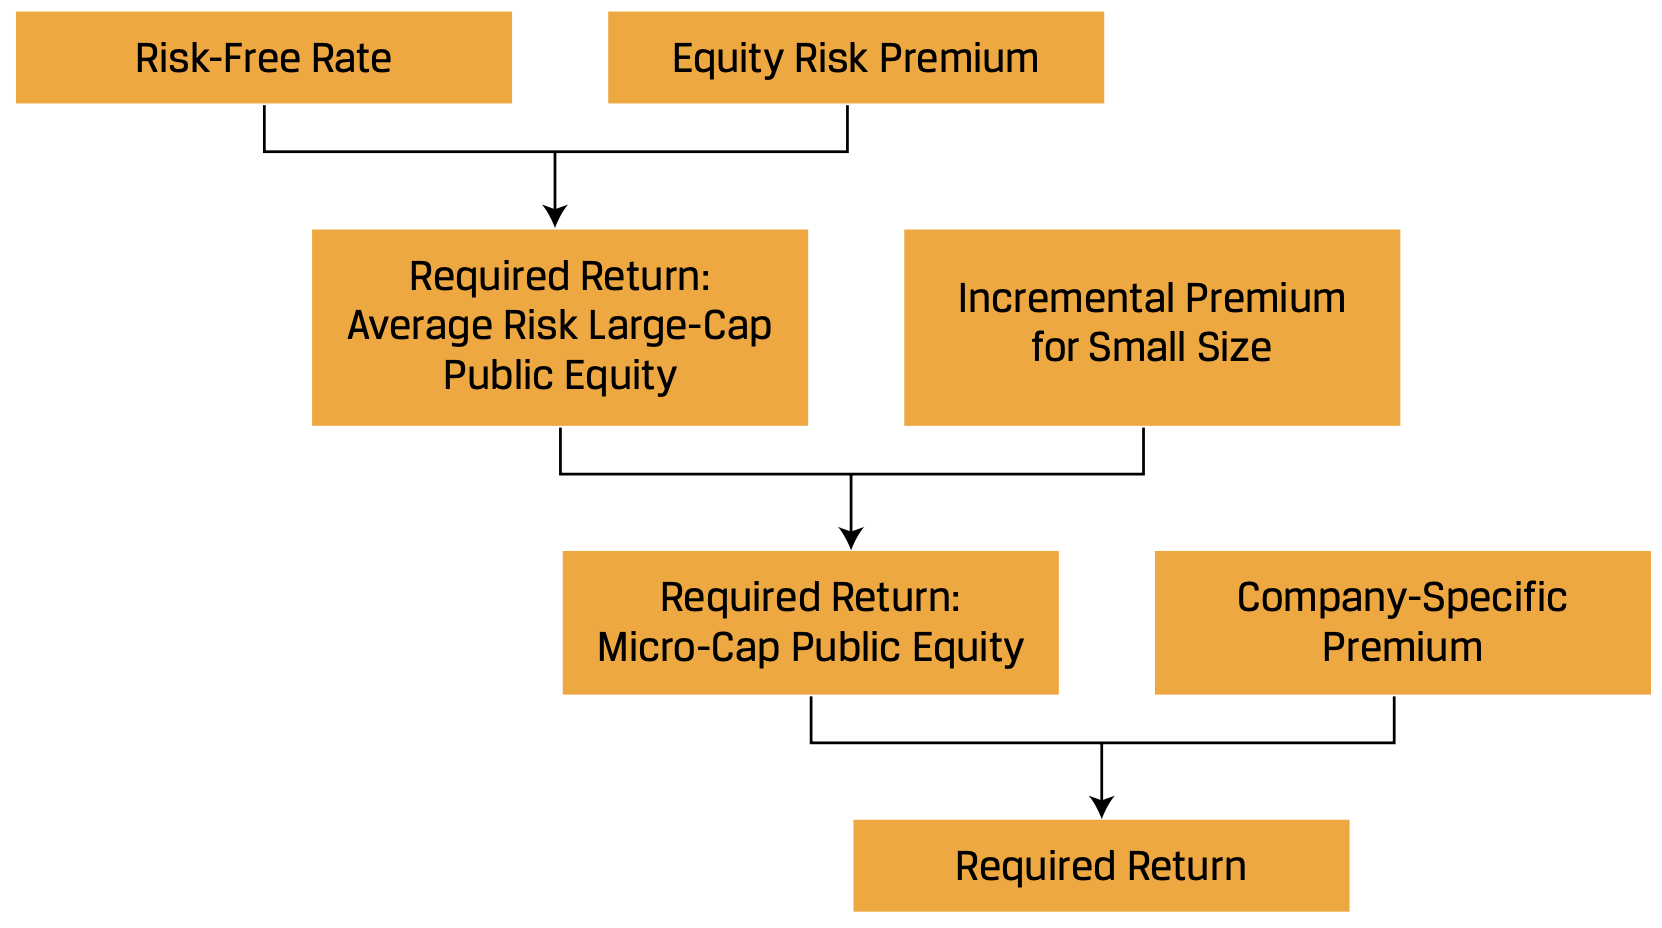
\includegraphics[scale=0.4]{/corpissuer/buildup}
\caption{Build-up approach for private companies.}
\end{figure}
Approach is suitable when set of comparable public companies are unavailable or incomparable.
\end{enumerate}
\end{method}

\begin{method} \hlt{ERP Estimation: International Considerations}\\
Risks for emerging market require additional premiums.
\begin{enumerate}[label=\roman*.]
\setlength{\itemsep}{0pt}
\item Country Spread Model: additional country risk premium (CRP) is to be added. The added risk could be due to economic conditions, risk of expropriation, political risk, or other risk.
\begin{equation}
\text{ERP}_{EM} = \text{ERP}_{DM} + (\lambda \times \text{CRP}) \nonumber
\end{equation}
where $\lambda$ is exposure of the company to the local company.\\
CRP is the premium associated with anticipated greater risk of market compared to benchmark developed market. Sovereign yield spread (yield difference in EM vs DM sovereign securities) may be used; but differences in legal and market environment complicates use of just yield spreads.\\
Aswath Damodaran suggests adjusting the sovereign yield spread by ratio of standard deviation of country's equity and bond markets as follows:
\begin{equation}
\text{CRP} = \text{Sovereign Yield Spread} \times \frac{\sigma_{\text{Equity}}}{\sigma_{\text{Bond}}} \nonumber
\end{equation}
\item Extended CAPM: for companies operating globally, two types of models may be used. If a company operations are global, GCAPM and ICAPM may both be used; however, if operations extend to EM, methodology is less clear (estimation using sovereign yield approach might be appropriate). \\
Global CAPM (GCAPM): global market index is used to estimate ERP. Beta coefficient usually quite low due to low correlation between EM and DM. A second factor representing the local market is sometimes included, but availability of reliable market index data is a concern in EM.\\
International CAPM (ICAPM): 2 factor model based on a global market index ($r_{gm}$) and a foreign currency-denominated, wealth-weighted market index ($r_c$):
\begin{equation}
E[r_e] = r_f + \beta_{G}[E[r_{gm}] - r_f] + \beta_{C}[E[r_c] - r_f] \nonumber
\end{equation}
The first factor of ICAPM captures company relationship with local economy relative to global economy (lower $\beta_{G}$ indicates lower integration of company with global economy). Second factor captures sensitivity of company CF to changes in its local currency value.\\
\end{enumerate}
\end{method}

\newpage

\subsection{Corporate Restructuring}



\newpage




\newpage

\section{Equity}

\subsection{Equity Valuation Application and Processes}

\begin{definition} \hlt{Intrinsic Value}\\
Valuation of an asset or security with complete understanding of the investment characteristic.
\end{definition}

\begin{definition} \hlt{Mis-pricing}\\
Difference between estimated intrinsic value and the market value of an asset.\\
Mis-pricing can be broken into true mis-pricing, and error in estimate of intrinsic value.
\begin{equation}
V_E - P = (V - P) + (V_E - V) \nonumber
\end{equation}
where $V_E$ is estimated intrinsic value, $V$ is actual intrinsic value, $P$ is market price.
\end{definition}

\begin{definition} \hlt{Going concern assumption} assumes that the company will continue to operate as a business.\\
\hlt{Going-concern value} of the company is its value under a going-concern assumption.\\
\hlt{Liquidation value} is value of the company if assets of the firm are sold separately, net company assets.
\end{definition}

\begin{definition} \hlt{Fair market value} is the price that a willing, informed, able seller will trade an asset to a similar buyer. Company's market price should reflect its fair market value over time if market has confidence that the management is acting in interest of equity investors.\\
\hlt{Investment value} is the value of a stock to a particular buyer, and is dependent on buyer's specific needs and expectations, and perceived synergies with existing buyer assets.\\
For most investment decisions, intrinsic value is relevant. For acquisitions, investment value is more appropriate.
\end{definition}

\begin{remark} The applications of equity valuation are as follows:
\begin{enumerate}[label=\roman*.]
\setlength{\itemsep}{0pt}
\item Stock selection: whether the security is fairly priced relative to estimated intrinsic value and comparables
\item Inferring market expectation: evaluate reasonableness of expectations implied by market price by comparing with market implied expectation. Market expectation for fundamentals may be useful as benchmark or comparison value of the same characteristic for another company.\\
To analyst market expectation, select a valuation model that relates value to fundamental expectations and is appropriate given characteristics of the stock. Next, estimate values for all fundamentals in the model except the fundamental of interest. Lastly, solve for the value of the fundamental of interest that results in the model value equal to the current market price.
\item Evaluating corporate events: assess how the events affect a company's cash flow and equity value. Also, in M\&A, as acquirer common stock is often used for purchase, to know if the stock is fairly valued.
\item Rendering fairness opinions: parties involved in merger may be required to seek a fairness opinion on terms of the merger from a third party, which will use valuation.
\item Evaluating business strategies and models: companies maximising shareholder value will evaluate effect of alternative strategies on share value.
\item Communication with analyst and investors: valuation provides target audience with a common basis to discuss and evaluate performance, current state, and future plans.
\item Appraising private businesses: to determine value of firms for transaction purposes and tax-reporting purposes, as well as to evaluate firm characteristics for IPOs.
\item Share-based payment: valuation for executive compensation.
\end{enumerate}
\end{remark}

\subsubsection{Valuation Process}

\begin{method} \hlt{Valuation Process Steps}
\begin{enumerate}[label=\arabic*.]
\setlength{\itemsep}{0pt}
\item Understanding the business: industry and competitive analysis, analysis of financial statements and other company disclosures.
\item Forecasting company performance: via forecast of sales, earnings, dividends, financial position (pro forma)
\item Selecting appropriate valuation model: depending on characteristics of company and context of valuation
\item Converting forecasts to a valuation: estimating value involves judgement
\item Applying valuation conclusions: for investment recommendations, provide opinion on price of transaction, or evaluate economic merits of potential strategic investment.
\end{enumerate}
\end{method}

\begin{remark} \hlt{Elements of Industry Structure} by Porter's Five Forces:
\begin{enumerate}[label=\arabic*.]
\setlength{\itemsep}{0pt}
\item Threat of new entrants
\item Threat of substitutes
\item Bargaining power of buyers
\item Bargaining power of suppliers
\item Rivalry among existing competitors
\end{enumerate}
Attractiveness (long-term profitability) is determined by interaction of these five competitive forces.
\end{remark}

\begin{remark} \hlt{Generic Strategies for Competing}
\begin{enumerate}[label=\roman*.]
\setlength{\itemsep}{0pt}
\item Cost leadership: being the lowest cost producer while offering comparable products.
\item Product differentiation: addition of product features or services to increase attractiveness of the firm's product so that it will command a price premium.
\item Focus: seeking a competitive advantage within a target segment or segments of the industry either through cost leadership or differentiation.
\end{enumerate}
Once a strategy has been identified, evaluate the performance of the business on how well it executes.
\end{remark}

\begin{flushleft}
Quality of Earnings Indicators
\begin{tabularx}{\textwidth}{p{7em}|p{18em}|X}
\hline
\rowcolor{gray!30}
Category & Observation & Potential Interpretation \\
\hline 
Revenue, gains & 
\xxx Recognising revenue early &
Boosts reported income, making a decline in operating performance \\
& 
\xxx Classification of non-operating income or gains as part of operations &
Income/gains non-recurring, not relate to true operating performance, masking declines in operating performance \\
\hline
Expenses, losses &
\xxx Recognising too much or too little reserves in current year &
Boost current income at expense of future income (or vice versa) \\
& 
\xxx Deferral of expenses by capitalising expenditures as asset &
Boost current income at expense of future income. Mask problems with underlying business performance \\
&
\xxx Aggressive estimates and assumptions &
May indicate actions taken to boost income. Changes in assumptions indicate attempt to mask problems with underlying performance in current period.\\
\hline
BS issues &
\xxx Use of off-BS financing, i..e, securitising receivables &
Assets and/or liabilities not properly reflected on BS \\
\hline
CFO &
\xxx Characterisation of an increase in bank overdraft as operating cash flow &
Operating cash flow artificially inflated \\
\hline
\end{tabularx}
\end{flushleft}

\begin{remark} \hlt{Warning Signs of Poor Earnings Quality}
\begin{enumerate}[label=\roman*.]
\setlength{\itemsep}{0pt}
\item Excessive pressure on employees to meet revenue target, combined with dominant, aggressive management
\item Management/director compensation tied to profitability or stock price
\item Economic, industry, or company-specific pressures on profitability
\item Management pressure to meet debt covenants or earnings expectations
\item Existence of related-party transactions
\item Complex organisational structure, where party in control is not apparent
\item High turnover of management, directors, or legal counsel
\item Reported (through regulatory filings) disputes with and/or changes in auditors
\item History of securities law violations, reporting violations, or persistent late filings
\end{enumerate}
\end{remark}

\begin{method} \hlt{Absolute Valuation Models}\\
Estimates asset intrinsic value based on investment characteristics.
\begin{enumerate}[label=\roman*.]
\setlength{\itemsep}{0pt}
\item Dividend Discount Models: estimate value of shares based on present value of all expected dividends discounted at opportunity cost of capital. Measure of cash flow may be expanded to include all expected cash flow to firm not payable to senior claims. These include free cash flow and residual income approach.
\item Asset-Based Models: estimates value of firm as sum of market value of assets it owns or controls. Used to value firms that own or control natural resources.
\end{enumerate}
\end{method}

\begin{method} \hlt{Relative Valuation Models}\\
Estimates asset value relative to other assets. Most common models use market price as a multiple of an individual financial factor, such as P/E ratio.
\end{method}

\begin{method} \hlt{Sum-of-Parts Valuation}\\
Value individual parts of a firm and add them up. Useful when company operates multiple divisions (or product lines) with different business models and risk characteristics (conglomerate).	
\end{method}

\begin{remark} \hlt{Conglomerate Discounts}\\
To markdown value of company that operates in multiple unrelated industries, as compared to value of company that has a single industry focus.
\begin{enumerate}[label=\roman*.]
\setlength{\itemsep}{0pt}
\item Internal Capital Inefficiency: company allocation of capital to different divisions may not have been based on sound decisions.
\item Endogenous (Internal) Factors: company may have pursued unrelated business acquisitions to hide poor operating performance
\item Research Measurement Errors: discount do not exist, and is a result of incorrect measurement
\end{enumerate}
\end{remark}

\begin{remark} \hlt{Criteria for Model Selection}
\begin{enumerate}[label=\roman*.]
\setlength{\itemsep}{0pt}
\item Consistent with characteristics of the company being valued
\item Appropriate given the availability and quality of data
\item Consistent with purpose of valuation, including analyst's perspective
\end{enumerate}
Multiple models are often used, and examining differences in estimated value can reveal how a model's assumption and perspective of the analysis affect the estimated values.
\end{remark}

\begin{flushleft}
Format for Research Reports
\begin{tabularx}{\textwidth}{p{10em}|X|X}
\hline
\rowcolor{gray!30}
Section & Purpose & Content \\
\hline 
Table of Contents &
\xxx Show report organisation, typically in long reports &
\xxx Consistent with narrative in sequence and language \\
\hline
Summary, Investment Conclusion &
\xxx Communicate large picture
\xxx Communicate major conclusions 
\xxx Recommend course of action &
\xxx Capsule description of company
\xxx Major recent developments
\xxx Earnings projections
\xxx Other major conclusions
\xxx Valuation summary
\xxx Investment action \\
\hline
Business Summary &
\xxx Present company in more detail
\xxx Communicate detailed understanding of company economics, situation
\xxx Provide and explain specific forecasts &
\xxx Description to divisional level
\xxx Industry analysis
\xxx Competitive analysis
\xxx Historical performance
\xxx Financial forecasts \\
\hline
Risks &
\xxx Alert readers to risk factors in investing in the security &
\xxx Negative industry developments
\xxx Negative regulatory, legal risks
\xxx Negative company developments
\xxx Risks in the forecasts
\xxx Other risks \\
\hline
Valuation & 
\xxx Communicate a clear and careful valuation &
\xxx Description of model used
\xxx Recapitulation of inputs
\xxx Statement of conclusions \\
\hline
Historical, Pro Forma Tables &
\xxx Organise and present data to support analysis in Business Summary\\
\hline
\end{tabularx}
\end{flushleft}


\newpage

\subsection{Discounted Dividend Valuations}

\begin{definition} \hlt{Dividends as Definition of Cash Flow}
\begin{enumerate}[label=\roman*.]
\setlength{\itemsep}{0pt}
\item Advantages: theoretically justified, as shareholder's investment today is worth the present value of future cash flows he expects to receive, which is repaid in form of dividends. Dividends are also less volatile than other measures, value estimates based on DDMs are less volatile and reflect long-term earning potential.
\item Disadvantages: not all firms pay dividends. Even by forecasting to the point when the firm is expected to begin paying dividends, there is uncertainty with forecasting that far into the future. Also, minority investors cannot control dividend policy. If dividend policy is not related to firm's ability to create value, then dividends are not an appropriate measure of expected cash flow to shareholders.
\end{enumerate}
Dividends are appropriate as measure of cash flow:
\begin{enumerate}[label=\roman*.]
\setlength{\itemsep}{0pt}
\item Company has history of dividends
\item Dividend policy is clear and related to earnings of the firm
\item Perspective is that of a minority shareholder
\end{enumerate}
Firms in mature stage are likely to meet first two criterial
\end{definition}

\begin{definition} \hlt{Free Cash Flow as Definition of Cash Flow}\\
FCFF is cash flow generated by operations in excess of capital investment required to sustain firm's current productive capacity. FCFE is cash available to shareholders after funding capital requirements and expenses associated with debt financing.
\begin{enumerate}[label=\roman*.]
\setlength{\itemsep}{0pt}
\item Advantage: may be applied to firms with different dividend policies or capital structures. Applicable to controlling shareholders as they may influence distribution and application of free cash flow. For minority shareholders, useful if firm is acquired for market price equal to value to controlling party.
\item Disadvantage: firms with significant capital requirements that may have negative FCF, caused by technological revolution in industry that requires greater investment to remain competitive, or by rapid expansion into untapped markets.
\end{enumerate}
FCF models are most appropriate:
\begin{enumerate}[label=\roman*.]
\setlength{\itemsep}{0pt}
\item For firms with no dividend payment history, or if dividend payment history is not related to earnings
\item For firms wth FCF that corresponds with their profitability
\item Perspective is that of a majority shareholder
\end{enumerate}
\end{definition}

\begin{definition} \hlt{Residual income as Definition of Cash Flow}\\
Earnings exceeding investor's required return.
\begin{enumerate}[label=\roman*.]
\setlength{\itemsep}{0pt}
\item Advantage: theoretically justified, as required return is the opportunity cost to suppliers of capital, and residual income is amount generated in excess of this return. Can be applied to firms with negative FCF and to dividend, and non-dividend paying firms.
\item Disadvantage: require in-depth analysis of accounting accruals, where there may be management discretion for both income and expense. If accounting is not transparent or if quality of firm's reporting is poor, accurate estimation of residual income is difficult.
\end{enumerate}
Residual income approach is most appropriate for:
\begin{enumerate}[label=\roman*.]
\setlength{\itemsep}{0pt}
\item firms with no dividend histories
\item firms with negative FCF for the foreseeable future, due to capital demands
\item firms with transparent financial reporting and high-quality earnings
\end{enumerate}
\end{definition}

\begin{definition} \hlt{Multiple Period Dividend Discount Model}
\begin{equation}
V_0 = \sum\limits_{t=1}^n \frac{D_t}{(1+r)^t} + \frac{P_n}{(1+r)^n} \nonumber
\end{equation}
where $V_0$ is value of share today, $P_n$ is expected price per share to time $n$, $D_t$ is expected dividend per share at end of year $t$, $r$ is required rate of return of stock. 
\end{definition}

\begin{definition} \hlt{Gordon Growth Model}\\
Assumes dividends increase at constant rate indefinitely. 
\begin{equation}
V_0 = \frac{D_0 \times (1+g)}{r-g} = \frac{D_1}{r-g} \nonumber
\end{equation}
where $g$ is expected constant growth rate, and $g < r$.\\
Firm's growth rate projection can be compared to growth rate of economy. Unrealistic to assume that any firm can grow indefinitely at rate higher than long-term growth rate in real GDP plus long-term inflation rate.\\
In general, perpetual dividend growth rate above $5\%$ is suspicious.\\
\end{definition}

\begin{remark} \hlt{Share Repurchases on DDM}\\
If companies have share repurchase programs, use total payout (dividends plus repurchases) in valuation model.\\
Alternatively, DDM focusing on cash dividends can be used after adjusting for number of shares outstanding, taking share repurchases into account.
\end{remark}

\begin{remark} \hlt{Value of Non-Callable Fixed-Rate Perpetual Preferred Stock (Capitalisation Rate)}\\
Firm with no additional opportunities to earn returns in excess of required rate of return should distribute all earnings to shareholders in form of dividends. Hence, growth rate will be zero.
\begin{equation}
V_0 = \frac{D}{r} \nonumber
\end{equation}
where $r$ is the discount rate that capitalises the amount $D$ (level dividend).
\end{remark}

\begin{remark} \hlt{Gordon Growth Model Strengths}
\begin{enumerate}[label=\roman*.]
\setlength{\itemsep}{0pt}
\item Applicable to stable, mature, dividend-paying firms
\item Appropriate for valuing market indices
\item Easily communicated and explained due to straightforward approach
\item Can be used to determine price-implied growth rate, required rates of return, value of growth opportunities
\item Can be used to supplement other more complex valuation methods.
\end{enumerate}
\end{remark}

\begin{remark} \hlt{Gordon Growth Model Weaknesses}
\begin{enumerate}[label=\roman*.]
\setlength{\itemsep}{0pt}
\item Valuations are very sensitive to estimates of growth rates and required rates of return
\item Model cannot be easily applied to non-dividend-paying stocks
\item Unpredictable growth patterns of some firms will make model valuations unreliable
\end{enumerate}
\end{remark}

\begin{remark} \hlt{Implied Growth Rates from Gordon Growth Model}\\
Price, current dividend may be observed for publicly traded stock.\\
Assuming a required return, we may calculate the implied growth rate. 
\begin{equation}
r = \frac{D_1}{P_0} + g \nonumber
\end{equation}
\end{remark}

\begin{remark} \hlt{Present Value of Growth Opportunities (PVGO)}\\
Firm with opportunities to earn in excess of required rate of return will retain earnings to invest in growth opportunities. The valuation will then have PVGO as an additional component.
\begin{equation}
V_0 = \frac{E_1}{r} + PVGO \nonumber
\end{equation}
where $E_1/r$ is the no-growth value per share.\\
Growth companies will have substantial portion of value in PVGO, while companies in slow-growth industries will have low PVGO, where most of their value comes from assets in place.
\end{remark}

\begin{remark} \hlt{Price to Earnings Ratio}\\
A justified P/E ratio is fair, warranted, or justified on the basis of fundamentals.
\begin{enumerate}[label=\roman*.]
\setlength{\itemsep}{0pt}
\item Justified Leading P/E: based on earnings forecast for next period.
\begin{equation}
\text{Justified Leading P/E} = \frac{P_0}{E_1} = \frac{D_1/E_1}{r-g} = \frac{1-b}{r-g} \nonumber
\end{equation}
\item Justified Trailing P/E: based on earnings for previous period.
\begin{equation}
\text{Justified Trailing P/E} = \frac{P_0}{E_0} = \frac{D_0(1+g)/E_1}{r-g} = \frac{(1-b)(1+g)}{r-g} \nonumber
\end{equation}
where $E_t$ is earnings at time $t$, $b$ is retention ratio, $(1-b)$ is dividend payout ratio.\\
Note that the price are the fundamental value of stock derived from Gordon Growth Model.\\
If earnings are expected to grow, $E_1 > E_0$, then the justified trailing P/E will be larger than the justified leading P/E due to the smaller denominator.
\end{enumerate}
\end{remark}

\begin{remark} \hlt{Growth Phases for Companies}\\
A justified P/E ratio is fair, warranted, or justified on the basis of fundamentals.
\begin{enumerate}[label=\roman*.]
\setlength{\itemsep}{0pt}
\item Growth Phase: firm has rapidly increasing earnings, little or no dividends, heavy reinvestment
\item Transition Phase: earnings and dividends still increasing but at a slower rate
\item Mature Phase: earnings grow at stable but slower rate, payout ratios are stabilising as reinvestment matches depreciation and asset maintenance requirements
\end{enumerate}
\end{remark}

\begin{flushleft}
\begin{tabularx}{\textwidth}{p{11em}|p{10.5em}|p{12em}|X}
\hline
\rowcolor{gray!30}
Variable & Growth & Transition & Mature \\
\hline 
Earnings Growth & Very High & Above average, decreasing & Stable at long-run level \\
\hline
Capital Investment & Significant requirements & Decreasing & Stable at long-run level \\
\hline
Profit Margin & High &  Above average, decreasing & Stable at long-run level \\
\hline
FCFE & Negative & Maybe position, growing & Stable at long-run level \\
\hline
ROE vs Required Return & $ROE > r$ & $ROE \rightarrow r$ & $ROE = r$ \\
\hline
Dividend Payout & Low or zero & Increasing & Stable at long-run level \\
\hline
Appropriate Model & Three-stage & Two-stage & Gordon Growth \\
\hline
\end{tabularx} 
\end{flushleft}

\begin{method} \hlt{Two-Stage DDM}\\
Company grows at high rate for relatively short period of time, then reverts to long-run perpetual growth rate.\\
Length of high-growth phase is function of visibility of company's operations.
\begin{equation}
V_0 = \sum\limits_{t=1}^n \frac{D_0 (1+g_S)^t}{(1+r)^t} + \frac{D_0 (1+g_S)^n (1+g_L)}{(1+r)^n (r-g_L)} \nonumber
\end{equation}
where $g_S$ is growth rate in stage one $g_L$ is growth rate in stage two.\\
For a firm that doesn't pay dividends, the first stage dividend is set to zero, then computed.
\end{method}

\begin{figure}[H]
\centering
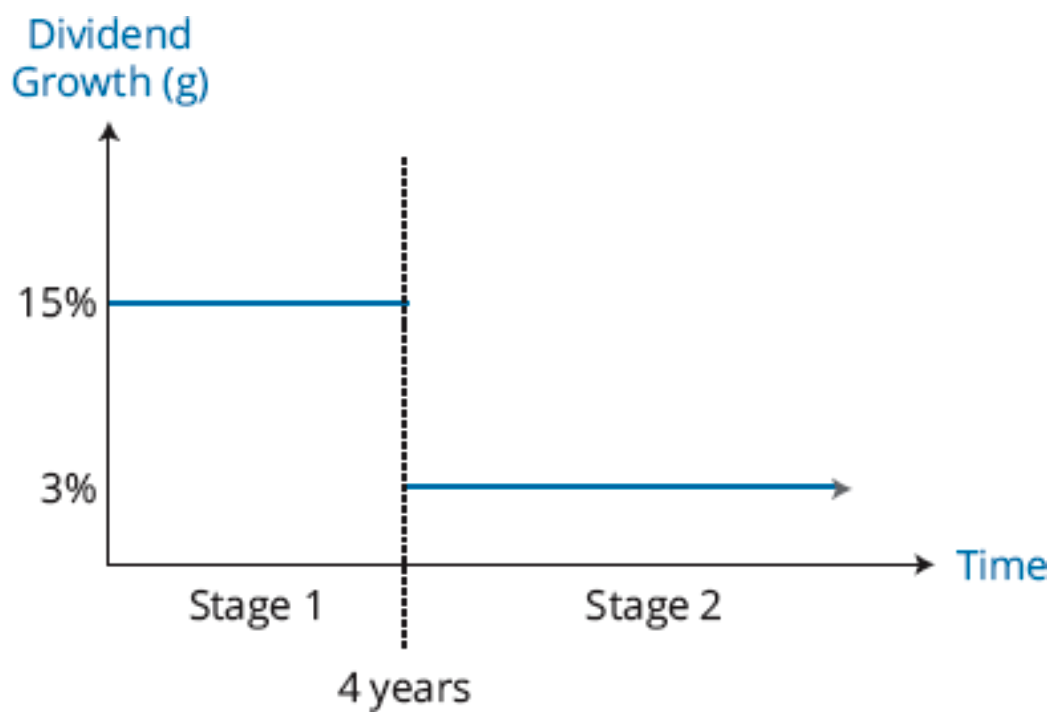
\includegraphics[scale=0.4]{images/equity/twostage}
\caption{Example of a two-stage model}
\end{figure}

\begin{method} \hlt{H-Model DDM}\\
Growth rate starts high, declines linearly over the high-growth stage until the long-run average growth rate.
\begin{equation}
V_0 = \frac{D_0 (1+g_L)}{r-g_L} + \frac{D_0 H (g_S - g_L)}{r-g_L} = \frac{D_0 (1+g_L) + D_0 H (g_S - g_L)}{r - g_L} \nonumber
\end{equation}
where $g_S$ is growth rate in stage one, $g_L$ is growth rate in stage two, $H$ is half-life in years of stage one.\\
The model may be rewritten to solve for $r$:
\begin{equation}
r = \frac{D_0}{P_0} [(1+g_L) + H(g_S - g_L)] + g_L \nonumber
\end{equation}
\end{method}

\begin{figure}[H]
\centering
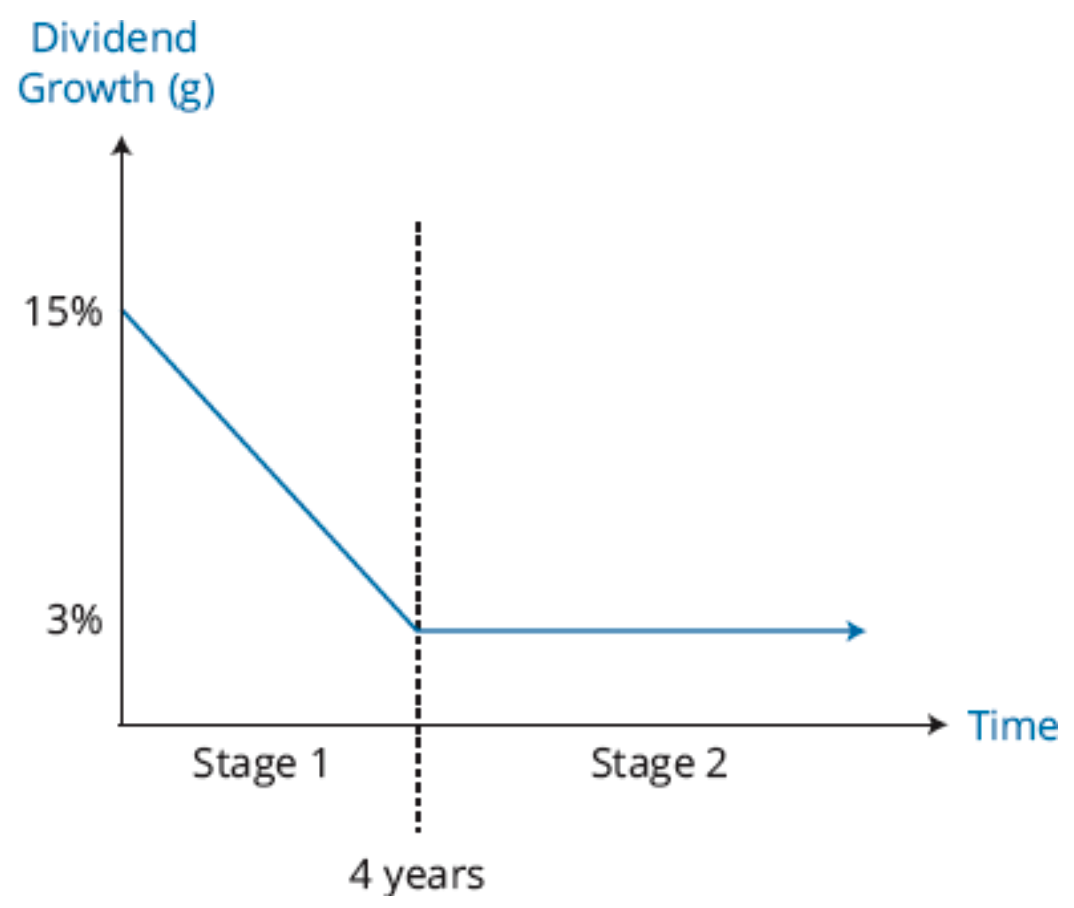
\includegraphics[scale=0.4]{images/equity/hmodel}
\caption{Example of a H-model}
\end{figure}

\begin{method} \hlt{Three-Stage Model DDM}\\
Firms that are expected to have three distinct stages of earnings growth.\\
More complex refinement of two-stage model. Process of using the model is as follows:
\begin{enumerate}[label=\roman*.]
\setlength{\itemsep}{0pt}
\item Gather the required inputs:
\begin{enumerate}[label=\arabic*.]
\setlength{\itemsep}{0pt}
\item the current dividend
\item estimate lengths of first, second, third stages and the expected growth rate in each stage
\item estimate of required return on equity
\end{enumerate}
\item compute the expected dividends in first stage and find sum of their present values. To investigate the company more deeply, such as explicit, individual earnings and dividend forecasts for the near future
\item apply H-model expression to second and third stages to obtain estimate of their value as beginning of second stage, then discount this H-value to as of $t=0$
\item sum the values obtained in the second and third steps
\end{enumerate}
\end{method}

\begin{figure}[H]
\centering
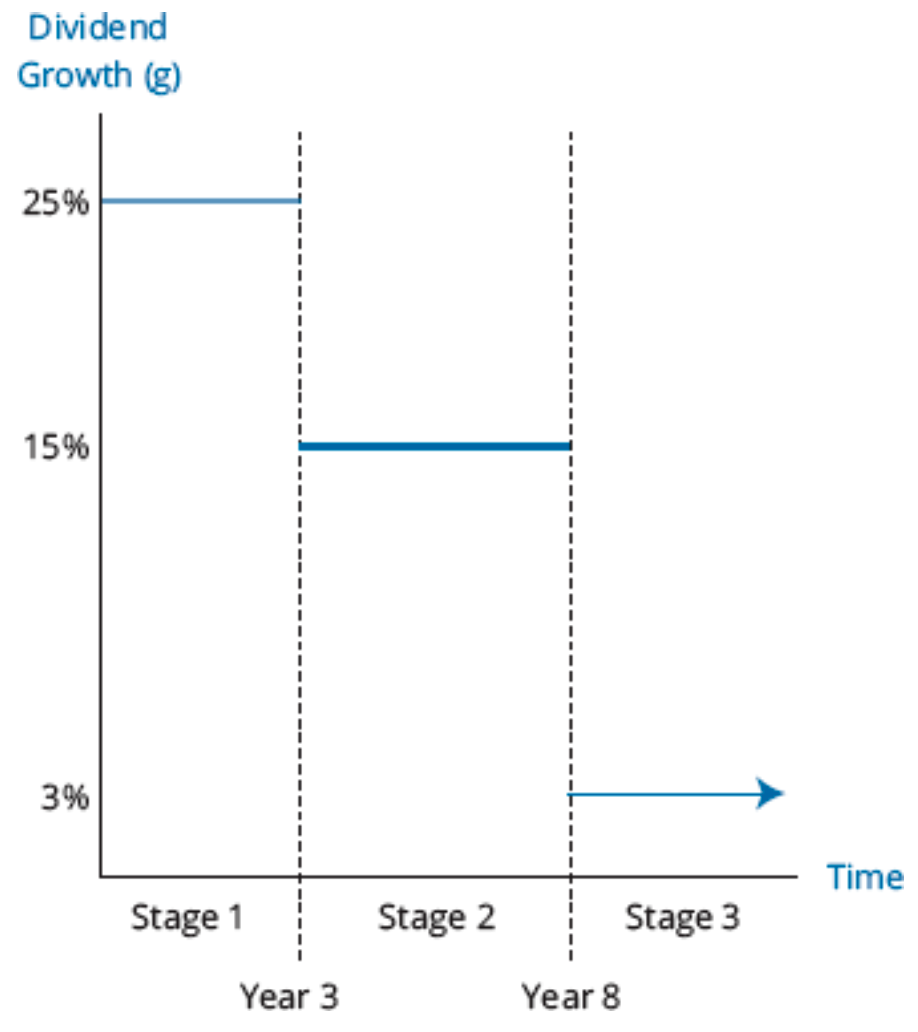
\includegraphics[scale=0.4]{images/equity/threestage}
\caption{Example of a three-stage model}
\end{figure}

\begin{method} \hlt{Terminal Value Estimation}
\begin{enumerate}[label=\roman*.]
\setlength{\itemsep}{0pt}
\item Gordon Growth Model: at some point in the future, assume dividends will grow at constant, long-term rate. The terminal value is then the value from Gordon Growth Model.
\item Market Price Multiples: forecast earnings and P/E ratio at the forecast horizon, then estimate the terminal value as the P/E multiplied by the earnings estimate.
\end{enumerate}
\end{method}

\begin{method} \hlt{Sustainable Growth Rate (SGR)}\\
Rate at which earnings (and dividends) can growth indefinitely, assuming debt-to-equity ratio is unchanged, and no new equity is issued.
\begin{equation}
SGD = b \times ROE \nonumber
\end{equation}
where $b$ is earnings return rate, equal to $1 - $ dividend payout rate.
\begin{enumerate}[label=\roman*.]
\setlength{\itemsep}{0pt}
\item Mature phase ROE may be estimated via:
\begin{enumerate}[label=\arabic*.]
\setlength{\itemsep}{0pt}
\item DuPont decomposition of ROE based on forecasts for components of DuPoint expression
\begin{align}
\text{ROE} &= \frac{\text{NI} - \text{Dividends}}{\text{NI}} \times \frac{\text{NI}}{\text{Sales}} \times \frac{\text{Sales}}{\text{Average assets}} \times \frac{\text{Average assets}}{\text{Average equity}} \nonumber
\end{align}
This is the \hlt{PRAT Model}, where SGR is function of profit margin (P), retention rate (R), asset turnover (A), financial leverage (T). Variables P and A are functions of performance, variables R and T are functions of financing decisions.\\
If actual growth rate is forecasted to be greater than SGR, the firm will have to issue equity unless the firm increases one of PRAT model factors.\\
For equity valuation, beginning-of-year BS values for mixed ratios are used.
\item Setting ROE $=r$, the require rate of return based on equity, on assumption that mature phase companies can do no more than earn investor's opportunity cost of capital
\item Setting ROE in mature phase equal to median industry ROE
\end{enumerate}
\item Relating $g$ to macroeconomic variables such as industry, growth, projections.
\end{enumerate}
\end{method}

\begin{definition} \hlt{Valuation of Stock}\\
If stock price is higher than model price, stock is overvalued.\\
If stock price is lower than model price, stock is undervalued.\\
If stock price is equal to model price, stock is fairly valued.
\end{definition}

\newpage

\subsection{Free Cash Flow Valuation}

\begin{definition} \hlt{Free Cash Flow to Firm (FCFF)}\\
Cash flow available to providers of capital after all operating expenses (including taxes, excluding interest expense), working capital investment and fixed capital investment has been made.
\end{definition}

\begin{definition} \hlt{Free Cash Flow to Equity (FCFE)}\\
Cash flow available to holders of common equity after all operating expenses, interest and principal payments have been paid, and investments in working and fixed capital has been made.
\end{definition}

\begin{remark} \hlt{FCFF vs FCFE Approach to Valuation}\\
In FCFF approach, value of firm is the value of discounted FCFF at WACC.\\
In FCFE approach, value of firm is the value of discounted FCFE at required rate of return for equity.\\
Both approaches should yield the same estimates if all inputs reflect identical assumptions.
\end{remark}

\begin{remark} \hlt{Circumstances of Using FCFF, FCFE}\\
If company capital structure is relatively stable, using FCFE is more direct and simpler than using FCFF.\\
However, there are two cases where FCFF model is chosen:
\begin{enumerate}[label=\roman*.]
\setlength{\itemsep}{0pt}
\item Levered company with negative FCFE. In this case, using FCFF would be the easiest.\\
Discount FCFF to find PV of operating assets, add value of excess cash (in relation to operating needs) and marketable securities and other significant non-operating assets to get total firm value. Then subtract market value of debt to obtain an estimate of intrinsic value of equity.
\item Levered company with changing capital structure. If historical data are used to forecast FCF growth rates, FCFF growth might reflect fundamentals more clearly than FCFE growth.\\
In addition, the required return on equity might be expected to be more sensitive to changes in financial leverage than changes in WACC, hence making the use of constant discount rate difficult to justify.
\end{enumerate}
\end{remark}

\begin{method} \hlt{Adjusted Present Value (APV) Approach}\\
Used when capital structure is expected to change.\\
Firm value is calculated as sum of:
\begin{enumerate}[label=\roman*.]
\setlength{\itemsep}{0pt}
\item un-levered firm value (assumes debt is not used) (discounted FCFF value at un-levered cost of equity)
\item NPV of any effects of debt on firm value (i.e., tax benefits of using debt and any costs of financial distress)
\end{enumerate}
\end{method}

\begin{method} \hlt{FCFF Valuation Approach}\\
Value of firm is PV of future FCFF discounted at WACC.
\begin{align}
\text{Firm Value} &= \sum\limits_{i=1}^{\infty} \frac{\text{FCFF}_t}{(1+\text{WACC})^t} \nonumber \\
\text{Equity Value} &= \text{Firm Value} - \text{MV}_{\text{Debt}} \nonumber \\
\text{WACC} &= \frac{\text{MV}_{\text{Debt}}}{\text{MV}_{\text{Debt}} + \text{MV}_{\text{Equity}}} r_d (1-t) + \frac{\text{MV}_{\text{Equity}}}{\text{MV}_{\text{Debt}} + \text{MV}_{\text{Equity}}}r \nonumber
\end{align}
where $r_d(1-t)$ is the after-tax cost of debt, $r$ is the after-tax cost of equity.
\end{method}

\begin{method} \hlt{FCFE Valuation Approach}\\
Value of firm is PV of future FCFE discounted at required rate of return on equity, $r$.
\begin{equation}
\text{Equity Value} = \sum\limits_{t=1}^{\infty} \frac{\text{FCFE}_t}{(1+r)^t} \nonumber
\end{equation}
\end{method}

\begin{method} \hlt{Constant Growth Models}\\
Assumes FCF grows at a constant rate.
\begin{enumerate}[label=\roman*.]
\setlength{\itemsep}{0pt}
\item FCFF Model: assumes FCFF grows at a constant rate $g$.
\begin{equation}
\text{Firm Value} = \frac{\text{FCFF}_1}{\text{WACC}-g} = \frac{\text{FCFF}_0 (1+g)}{\text{WACC} - g} \nonumber
\end{equation}
\item FCFE Model: assumes FCFE grows at constant rate $g$.
\begin{equation}
\text{Equity Value} = \frac{\text{FCFE}_1}{r-g} = \frac{\text{FCFE}_0 (1+g)}{r - g} \nonumber \end{equation}
\end{enumerate}
\end{method}

\begin{method} \hlt{Computing FCFF from Net Income}
\begin{equation}
\text{FCFF} = \text{NI} + \text{NCC} + \text{Int}(1-t) - \text{FCInv} - \text{WCInv} \nonumber
\end{equation}
where NI is net income, NCC is net non-cash charges, Int is interest expense, FCInv is fixed capital investment, WCInv is working capital investment.\\
\end{method}

\begin{remark} \hlt{Non-Cash Charges Treatment for FCFF}\\
Expenses that reduce reported net income but do not involve cash inflows or outflows.
\begin{flushleft}
\begin{tabularx}{\textwidth}{p{28em}|X}
\hline
\rowcolor{gray!30}
Non-Cash Item & Adjustment to NI to arrive at FCFF\\
\hline
Depreciation expense & Added back \\
\hline
Amortisation expense, impairment of intangibles & Added back \\
\hline
Restructuring charges (expense) & Added back \\
\hline
Restructuring charges (income from reversal) & Subtracted \\
\hline
Amortisation of long-term bond discounts & Added back \\
\hline
Amortisation of long-term bond premiums & Subtracted \\
\hline
Losses on non-operating activity (i.e., long-term assets) & Added back \\
\hline
Gains on non-operating activity (i.e., long-term assets) & Subtracted \\
\hline
Deferred taxes (increases of non-reversible deferred tax liabilities) & Added back \\
\hline
Deferred taxes (increases of non-reversible deferred tax assets) & Subtracted \\
\hline
\end{tabularx}
\end{flushleft}
\end{remark}

\begin{method} \hlt{Fixed Capital Investment Treatment for FCFF}\\
Not on IS, but represent outflow of cash, hence to remove from net income to estimate FCFF.
\begin{equation}
\text{FCInv} = \text{Capex} - \text{Proceeds from sales of long-term assets} \nonumber
\end{equation}
\begin{enumerate}[label=\roman*.]
\setlength{\itemsep}{0pt}
\item If no long-term assets were sold during the year:
\begin{equation}
\text{FCInv} = \text{PP\&E}_{End} - \text{PP\&E}_{Beginning} + \text{Depreciation} -\text{Gain on Sale} \nonumber
\end{equation}
\item If long-term assets were sold during the year, then
\begin{enumerate}[label=\arabic*.]
\setlength{\itemsep}{0pt}
\item Determine Capex from CFS, i.e., 'Purchase of fixed assets', or 'Purchase of PP\&E' under CFI
\item Determine proceeds from sales of fixed assets from CFS, i.e., 'Proceeds from disposal or fixed assets'
\item Compute with the first equation of FCInv
\item If Capex or sales proceeds are not given directly, find gain/loss on asset sales from IS and PP\&E figures from BS. Compute with the second equation of FCInv.
\end{enumerate}
\end{enumerate}
\end{method}

\begin{method} \hlt{Working Capital Investment Treatment for FCFF}
\begin{equation}
\text{WCInv} = \Delta\text{Working Capital} - \text{Cash} - \text{Cash Equiv} - \text{Notes Payable} - \text{Current portion of LT Debt} \nonumber
\end{equation}
Note that if working capital has a reduction, this will be added back as it is a cash inflow.
\end{method}

\begin{method} \hlt{Interest Expense Treatment for FCFF}\\
A financing CF to bondholders, available to the firm before it makes any payments to capital suppliers.\\
Only add after-tax interest expense, as paying interest reduces the tax bill.
\end{method}

\begin{flushleft}
\begin{tabularx}{\textwidth}{p{22em}|X}
\hline
\rowcolor{gray!30}
Statement of Cash Flows & FCFF, FCFE \\
\hline
Net Income (NI) & Net Income (NI) \\
$+$ Non-Cash Charges (NCC) & $+$ Non-Cash Charges (NCC) \\
\underline{$-$ WCInc} & \underline{$-$ WCInc} \\
Cash Flow from Operations (CFO) & Cash Flow from Operations (CFO) \\
& \hlt{$+$ Int(1-t)} \\
\underline{$-$ FCInc} & \underline{$-$ FCInc} \\
(Almost) FCFF & (Actual) FCFF \\
$+$ Net Borrowing & $+$ Net Borrowing  \\
& \hlt{$-$ Int(1-t)} \\
FCFE & FCFE \\
$-$ Dividends & $-$ Dividends \\
\underline{$\pm$ Common Stock Issues (Repurchases)} & \underline{$\pm$ Common Stock Issues (Repurchases)} \\
Net Change in Cash & Net Change in Cash\\
\hline
\end{tabularx}
\end{flushleft}

\begin{method} \hlt{Computing FCFF, FCFE from CFO}\\
Depreciation is added back in full as it will be claimed in taxes, but doesn't represent an actual cashflow.\\
Interest is not added back in full; by retaining the cash, there will be lower interest expense and higher tax.
\begin{enumerate}[label=\roman*.]
\setlength{\itemsep}{0pt}
\item Compute almost FCFF:
\begin{align}
\text{Almost FCFF} &= (\text{NI} + \text{NCC} - \text{WCInv}) - \text{FCInv} \nonumber \\
&= \text{CFO} - \text{FCInv} \nonumber
\end{align}
\item As interest expense is an CFO, but to reclassify as CFF, and this is tax deductible, to add it back to NI then subtract it out as CFF outflow. We may then have the actual FCFF:
\begin{align}
\text{Actual FCFF} &= (\text{NI} + \text{NCC} - \text{WCInv}) + \text{Int}(1-t) - \text{FCInv} \nonumber \\
&= \text{CFO} + \text{Int}(1-t) - \text{FCInv} \nonumber
\end{align}
\end{enumerate}
Note that any financial decisions that affect cash flows below FCFE (dividends, share repurchases, share issues etc) do not affect FCFF or FCFE.
\end{method}

\begin{method} \hlt{Computing FCFF from EBIT}\\
Starting with EBIT, add back depreciation as it was subtracted out to get EBIT.\\
As EBIT is before interest and taxes, do not have to remove interest (as it is CFF).\\
Note that non-cash adjustments occur on IS below EBIT, do not have to adjust for them when calculating FCF starting with EBIT. The only non-cash charge that appears above EBIT is depreciation.
\begin{equation}
\text{FCFF} = \text{EBIT}(1-t) + \text{Dep} - \text{FCInv} - \text{WCInv} \nonumber
\end{equation}
\end{method}

\begin{method} \hlt{Computing FCFF from EBITDA}\\
EBITDA is before depreciation, hence to add back depreciation tax shield.\\
Even though depreciation is non-cash expense, firm reduces its tax bill by expensing it.
\begin{equation}
\text{FCFF} = \text{EBITDA}(1-t) + \text{Dep}(t) - \text{FCInv} - \text{WCInv} \nonumber
\end{equation}
\end{method}

\begin{method} \hlt{Computing FCFE from FCFF}\\
Starting with FCFF, adjust for two cashflows to bondholders: after-tax interest expense, and any ST and LT borrowings. To subtract after-tax interest expense as paying interest reduces tax bill and reduces cash available to shareholders by interest paid minus the taxes saved.
\begin{equation}
\text{FCFE} = \text{Actual FCFF} - \text{Int}(1-t) + \text{Net Borrowing} \nonumber\text{FCFE} = \text{Actual FCFF} - \text{Int}(1-t) + \text{Net Borrowing} \nonumber
\end{equation}
\end{method}

\begin{method} \hlt{Computing FCFE from CFO}\\
Difference from FCFF is that after-tax interest expense is not aded back, and net borrowing is added back.
\begin{align}
\text{Actual FCFE} &= (\text{NI} + \text{NCC} - \text{WCInv}) - \text{FCInv} + \text{Net Borrowing} \nonumber \\
&= \text{CFO} - \text{FCInv} + \text{Net Boorrowing} \nonumber
\end{align}
\end{method}

\begin{method} \hlt{Treatment of FCF with Preferred Stock}\\
Treat preferred stock like debt, except preferred dividends are not tax deductible.\\
Any preferred dividends should be added back to FCF (approach assumes this is NI to common stockholders).\\
WACC to be revised to reflect percent of total capital raised by preferred stock as cost of that capital source.\\
FCFE to modify net borrowing to reflect new debt borrowing and net issuances by amount of preferred stock.
\end{method}

\begin{method} \hlt{Uses of CF to Verify FCFF, FCFE}\\
Uses of CF may be used to verify FCFF and FCFE as follows.
\begin{flushleft}
\begin{tabularx}{\textwidth}{p{22em}|X}
\hline
\rowcolor{gray!30}
Uses of FCFF $=$ & Uses of FCFE $=$ \\
\hline
\ \ \ Changes in Cash Balances & \ \ \ Changes in Cash Balances \\
$+$ Net Payments to Debt Providers & \\
\ \ \ ($+$ Int$(1-t)$ & \\
\ \ \ \ $+$ principal payment excess of net borrowing) &  \\
$+$ Net Payments to Equity Stakeholders & $+$ Net Payments to Equity Stakeholders \\
\ \ \ ($+$ cash dividends & \ \ \ ($+$ cash dividends \\
\ \ \ \ $+$ share repurchase excess of share issuance) & \ \ \ \ $+$ share repurchase excess of share issuance) \\
\hline
\end{tabularx}
\end{flushleft}
\end{method}

\begin{method} \hlt{Forecasting FCFF and FCFE}
\begin{enumerate}[label=\roman*.]
\setlength{\itemsep}{0pt}
\item Historical Cash Flow: apply constant growth rate with same relationship with fundamental factors.
\item Components-Based Projection: sales-based forecasting method, based on assumption that (FCInv - Dep) and WCInv has constant relationship to increases in size of company measured by increase in sales.\\
If depreciation reflects annual cost for maintaining existing capital stock, incremental FCInv should be related to Capex required for growth. The inputs needed are then:
\begin{enumerate}[label=\arabic*.]
\setlength{\itemsep}{0pt}
\item forecast of sales growth rates;
\item forecasts of after-tax operating margin (FCFF) or profit margin (FCFE)
\item estimate of relationship of incremental FCInv to sales increases
\item estimate of relationship of WCInv to sales increases
\item estimate of debt ratio
\end{enumerate}
For FCFE forecasting, forecast EBIT$(1-t)$ and subtract incremental FCInv and WCInv.\\
To estimate FCInv and WCInv, multiple past proportion to sales increases by forecasted sales increases.
\begin{align}
\text{Incremental FCInv} &= \frac{\text{Capex} - \text{Depreciation expense}}{\text{Increase in sales}} \nonumber \\
\text{Incremental WCInv} &= \frac{\text{Increase in working capital}}{\text{Increase in sales}} \nonumber
\end{align}
When depreciation is the only significant net non-cash charge, this yields same result as previous equations for estimating FCFF or FCFE.  This approach simply subtracts net Capex in excess of depreciation.\\
For forecasting FCFE, assume that a specified percentage of sum of new investment in fixed capital and increase in working capital is financed based on target debt ratio.
\begin{align}
\text{FCFE} &= \text{NI} - (\text{FCInv} - \text{Dep}) - \text{WCInv} + \text{Net borrowing} \nonumber
\end{align}
By assuming a target debt ratio, net borrowing will not be forecasted.
\begin{align}
\text{Net borrowing} = DR(\text{FCInv} - \text{Dep}) + DR(\text{WCInv}) \nonumber
\end{align}
Hence, debt issuance and repayment on annual basis will not be forecasted.
\begin{align}
\text{FCFE} &= \text{NI} - (\text{FCInv} - \text{Dep}) - \text{WCInv} + DR(\text{FCInv} - \text{Dep}) + DR(\text{WCInv}) \nonumber \\
\text{FCFE} &= \text{NI} - (1 - DR)(\text{FCInv} - \text{Dep}) - (1-DR)(\text{WCInv}) \nonumber
\end{align}
\end{enumerate}
\end{method}

\begin{remark} \hlt{Effect of Financing Decisions on FCF}\\
Dividends and share repurchases are uses of CF, hence do not affect level of CF available.
\begin{flushleft}
\begin{tabularx}{\textwidth}{p{12em}|X|X}
\hline
\rowcolor{gray!30}
Financing Decisions & FCFF & FCFE \\
\hline
Dividends & None & None \\
Share repurchase & None & None \\
Share issue & None & None \\
Change in leverage & None & ST and LT effects partially offset$^{*}$\\
\hline
\end{tabularx}
($^{*}$) Decrease in leverage through repayment of debt will decrease FCFE in current year and increase forecasted FCFE in future years as interest expense is reduced.
\end{flushleft}
\end{remark}

\begin{remark} \hlt{FCFE vs DDM}\\
FCFE approach takes a control perspective, assumes recognition of value should be immediate.\\
DDM take minority perspective, value not be recognised until dividend policy affects firm's long-run profitability.
\end{remark}

\begin{remark} \hlt{Net Income as Proxy for FCFE}\\
Net income includes non-cash charges like depreciation that have to be added back to arrive at FCFE.\\
Net income ignores CF that don't appear on IS, such as WCInv and FCInv, Net Borrowings.
\begin{equation}
\text{FCFE} = \text{NI} + \text{NCC} - \text{FCInv} - \text{WCInv} + \text{Net Borrowing} \nonumber
\end{equation}
\end{remark}

\begin{remark} \hlt{EBITDA as Proxy for FCFF}\\
EBITDA doesn't reflect cash taxes paid by firm, and ignores CF effects of WCInv and FCInv.
\begin{equation}
\text{FCFF} = \text{EBITDA}(1-t) + (\text{Dep})t - \text{FCInv} - \text{WCInv} \nonumber
\end{equation}
\end{remark}

\begin{remark} \hlt{Sources of Error in Valuation Analysis}
\begin{enumerate}[label=\roman*.]
\setlength{\itemsep}{0pt}
\item Estimation of future growth in FCFF and FCFE. Growth forecasts depend on firm's future profitability, which depends on sales growth, changes in profit margin, position in life cycle, competitive strategy, and overall profitability of the industry.
\item Chosen base years for FCFF, FCFE growth forecasts. Representative base year to be chosen, or all of the subsequent analysis and valuation will be flawed.
\end{enumerate}
\end{remark}

\newpage

\newpage

\section{Fixed Income}

\subsection{Fundamentals of Fixed Income}

\begin{figure}[H]
\centering
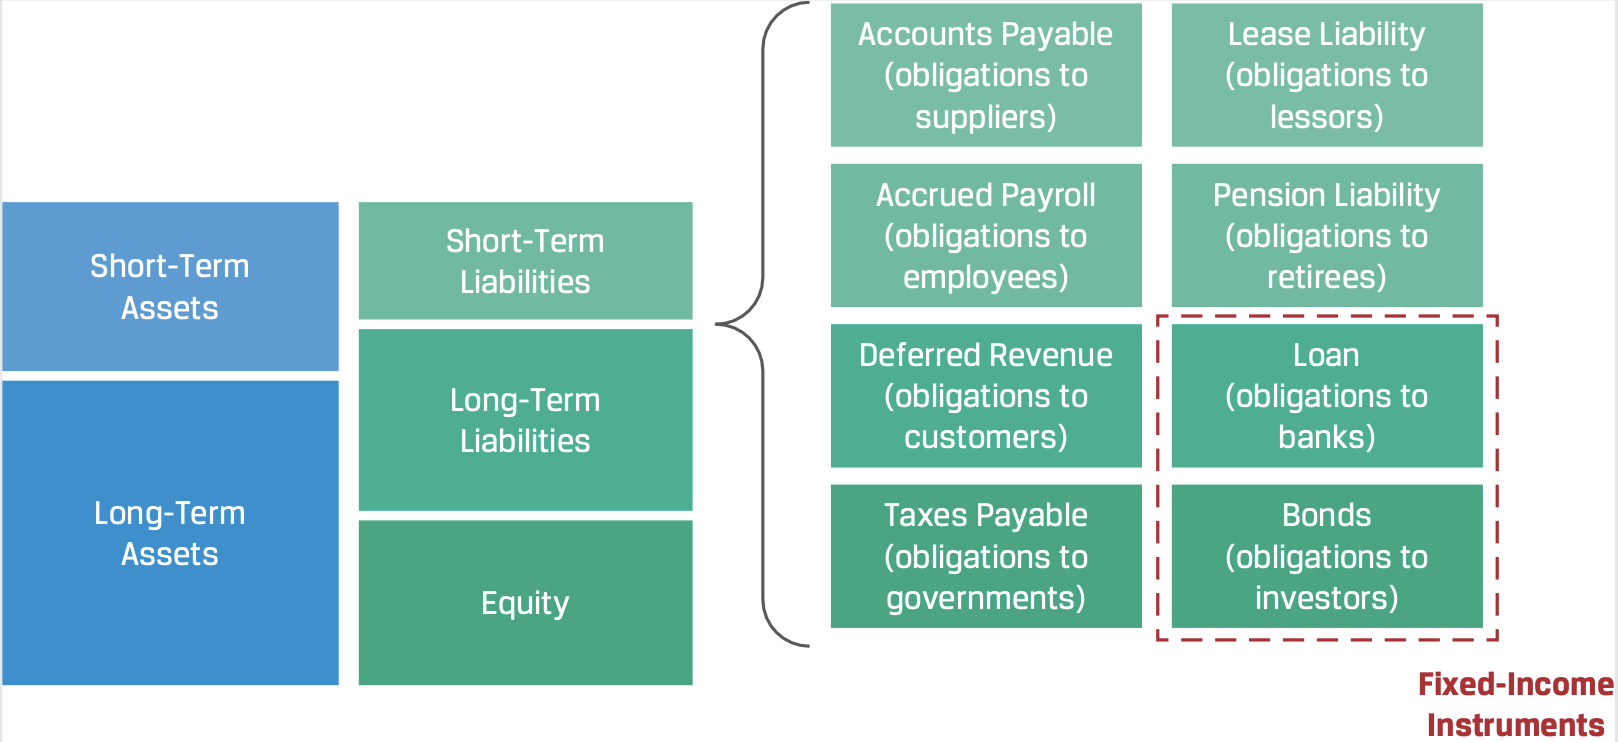
\includegraphics[scale=0.4]{/fi/fiscope}
\caption{Scope of fixed income instruments}
\end{figure}

\begin{remark} Issuers of Fixed Income
\begin{enumerate}[label=\roman*.]
\setlength{\itemsep}{0pt}
\item Supranational Organisations: World Bank, European Bank
\item Government Bonds: sovereign (national), non-sovereign (local), quasi-national (agencies)
\item Corporate: from financial and non-financial firms
\item Special Legal Entities: securitise assets for asset-backed securities (ABS)
\end{enumerate}
\end{remark}

\begin{remark} Common Terminology
\begin{enumerate}[label=\roman*.]
\setlength{\itemsep}{0pt}
\item Maturity: date of final payment the issuer makes to investors
\item Tenor: remaining time to maturity
\item Par Value: amount issuer agrees to pay the bondholder on the maturity date, quoted on $100$-point system
\item Market Reference Rate: standard borrowing or lending rate for issuers with lowest default risk for different currencies and maturities.
\end{enumerate}
\end{remark}

\begin{remark} \hlt{Classification of Fixed Income by Maturity}
\begin{enumerate}[label=\roman*.]
\setlength{\itemsep}{0pt}
\item Money Market Security: maturity at issuance less than $1$ year
\item Capital Market Security: maturity at issuance greater than $1$ year
\item Perpetual Bonds: bond type with no stated maturity
\end{enumerate}
\end{remark}

\begin{remark} \hlt{Classification of Fixed Income by Coupon Rate and Frequency}
\begin{enumerate}[label=\roman*.]
\setlength{\itemsep}{0pt}
\item Floating-Rate Notes (FRNs): market reference rate (MRR) with issuer-specific credit spread.
\item Quarterly Income Debt Security (QUIDS): senior unsecured debt issued in small denominations with long maturities, interest paid quarterly.
\end{enumerate}
\end{remark}

\newpage

\subsection{Fixed Income Valuation}

\begin{definition} \hlt{Time Value of Money}
\begin{equation}
PV = \sum\limits_{t=1}^N \frac{PMT}{(1+r)^t} + \frac{FV}{(1+r)^N} \nonumber
\end{equation}
where $PV$ is present value of bond, $PMT$ is coupon payment, $FV$ is face value, $r$ is required rate of return.\\
\end{definition}

\begin{definition} \hlt{Yield to Maturity (YTM)}\\
Time value of money equation may be modified to solve for $r$ (internal rate of return on cash flows). This is the implied or observed single market discount rate. Assumes the following:
\begin{enumerate}[label=\roman*.]
\setlength{\itemsep}{0pt}
\item Investor holds bond to maturity
\item All coupon and principal payments are on scheduled dates
\item Investor is able to reinvest coupon payments at the same yield
\end{enumerate}
\end{definition}

\begin{definition} \hlt{Horizon Yield}\\
Internal rate of return between total return and purchase price of bond.\\
The horizon yield on a bond investment is the annualised holding-period rate of return.
\end{definition}

\subsubsection{Pricing of Fixed Income}

\begin{definition} \hlt{Flat Price, Accrued Interest, Full Price}\\
When bond is priced between coupon payment dates, its price has two components: the flat price $PV^{\text{Flat}}$, and the accrued interest $AI$. Sum of the parts is the full price $PV^{\text{Full}}$.
\begin{align}
PV^{\text{Full}} &= PV^{\text{Flat}} + AI \nonumber \\
AI &= \frac{t}{T} \times PMT \nonumber
\end{align}
where $t$ is number of days from prior coupon payment to settlement date, $T$ is number of days in coupon period.
\end{definition}

\begin{figure}[H]
\centering
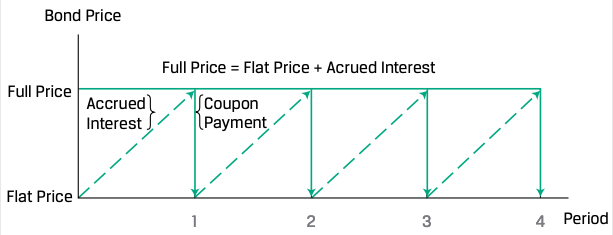
\includegraphics[scale=0.4]{/fi/fullprice}
\caption{Full price of the bond}
\end{figure}

\begin{remark} \hlt{Conventions for Day Counting}\\
Specified by two parameters: how days are counted in a given period, and the number of days assumed per period. Common conventions are $30/360$ and Actual$/$Actual
\end{remark}

\begin{remark} \hlt{Full Price and Payment}\\
Full price of fixed-rate bond between coupon payments, given by market discount rate per period $r$, is present value of future cash flows as of trade settlement ate.
\begin{align}
PV^{\text{Full}} &= \sum\limits_{n=1}^N \frac{PMT}{(1+r)^{n-t/T}} + \frac{FV}{(1+r)^{N-t/T}} \nonumber \\
&= \left[ \sum\limits_{n=1}^N \frac{PMT}{(1+r)^{n}} + \frac{FV}{(1+r)^{N}} \right] \times (1+r)^{t/T} \nonumber \\
&= PV \times (1+r)^{t/T} \nonumber
\end{align}
\end{remark}


\begin{remark} \hlt{Quotation for Bonds}\\
On a basis-point ($100$-point) system, i.e., $@106$ means $106\%$ of face value.\\
If coupon rate $<$ market discount rate, then $PV < 100$, the bond is at a discount.\\
If coupon rate $=$ market discount rate, then $PV = 100$, the bond is at par.\\
If coupon rate $>$ market discount rate, then $PV > 100$, the bond is at a premium.
\end{remark}

\begin{remark} \hlt{Price and Interest Rate Relationship}\\
Bond prices and interest rates are inversely related. Price decreases as interest rate increases.
\end{remark}

\begin{remark} \hlt{Spot Rate Pricing}\\
Spot rate is the yield-to-maturity on zero-coupon bonds.\\
Calculate with sequence of market discount rates corresponding to the CF dates.
\begin{equation}
PV = \sum\limits_{t=1}^N \frac{PMT}{(1+Z_t)^{t}} + \frac{FV}{(1+Z_N)^{N}} \nonumber
\end{equation}
where $Z_t$ is the spot rate/zero-coupon yield for period $t$.
\end{remark}

\begin{remark} \hlt{Bond Relationships}
\begin{enumerate}[label=\roman*.]
\setlength{\itemsep}{0pt}
\item Inverse Relationship: bond prices and interest rates are inversely related.\\
Price decreases as interest rate increases.
\item Convexity Effect: for the same coupon rate and time-to-maturity, $\abs{\% \Delta \text{Price}}_{r \downarrow} > \abs{\% \Delta \text{Price}}_{r \uparrow}$.\\
Prices are more volatile on the upside for a $1\%$ change in interest rate.
\item Coupon Effect: given same time-to-maturity, lower-coupon bond has greater $\% \Delta$ Price than higher-coupon bond for same change in market discount rates.
\item Maturity effect: given same coupon rate, longer-term bond has greater $\% \Delta$ Price than shorter-term bond for same change in market discount rates. May not hold for low-coupon, long-term discount bonds
\end{enumerate}
\end{remark}

\begin{figure}[H]
\centering
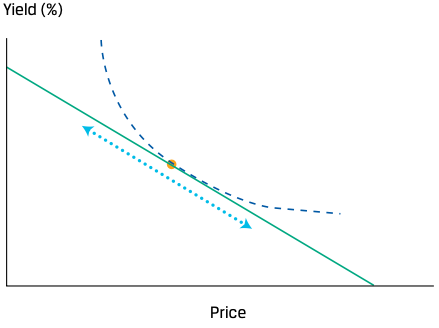
\includegraphics[scale=0.4]{/fi/convexpyrel}
\caption{Convex Price-Yield Relationship}
\end{figure}

\begin{remark} \hlt{Constant-Yield Price Trajectory}\\
As time passes, bondholder comes closer to receiving par value at maturity.\\
Price of bond approaches par value as its time-to-maturity approaches zero.\\
Carrying value is purchase price plus amortised amount of discount if purchased below par value, or minus amortised amount of premium if purchased above par value.
\end{remark}

\begin{figure}[H]
\centering
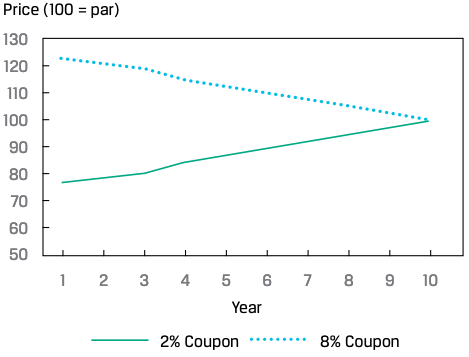
\includegraphics[scale=0.4]{/fi/constpricetraj}
\caption{Constant-Yield Price Trajectory}
\end{figure}

\begin{remark} Purpose of Matrix Pricing\\
To price illiquid or new fixed-rate bonds.\\
Underwriting new bonds to get an estimate of the required yield spread over the benchmark rate.\\
Estimate market discount rate and price based on quoted or flat prices of more frequently traded comparable bonds, with similar time-to-maturity, coupon rates, and credit quality.
\end{remark}

\begin{method} \hlt{Determining Price of New or Illiquid Bond with Matrix Pricing}
\begin{enumerate}[label=\roman*.]
\setlength{\itemsep}{0pt}
\item Identify actively traded, comparable bonds with similar times-to-maturity, coupon rates, credit quality.
\item Calculate YTM for each comparable bonds, and calculate average yield for each maturity year.
\item Linearly interpolate the YTMs of comparable bonds to estimate YTM closest to target bond maturity.
\item Using estimated YTM, calculate price of new/illiquid bond by discounting all coupon and principal.
\end{enumerate}
\end{method}

\begin{figure}[H]
\centering
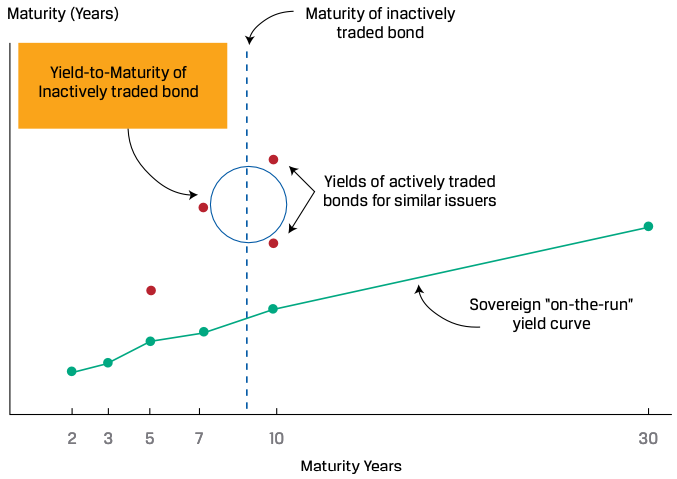
\includegraphics[scale=0.45]{/fi/matrixprice}
\caption{Matrix Pricing}
\end{figure}

\begin{remark} \hlt{Spread over the Benchmark}\\
Used in underwriting new bonds to get an estimate of required yield spread over benchmark rate.\\
Benchmark rate is the YTM on government bond with similar time-to-maturity.\\
Spread (over the benchmark) is the difference between YTM on new bond and benchmark rate.\\
Spread is the additional compensation to account for difference in credit risk, liquidity risk, tax status of bond relative to government bond.
\end{remark}

\subsubsection{Yield and Yield-Spread Measures for Fixed-Rate Instruments}

\begin{definition} Yield Rate Terminologies 
\begin{enumerate}[label=\roman*.]
\setlength{\itemsep}{0pt}
\item \hlt{Semiannual Bond Basis/Equivalent Yield}: annual rate with periodicity of two.
\item \hlt{Effective Annual Rate}: rate with periodicity of one.
\end{enumerate}
\end{definition}

\begin{figure}[H]
\centering
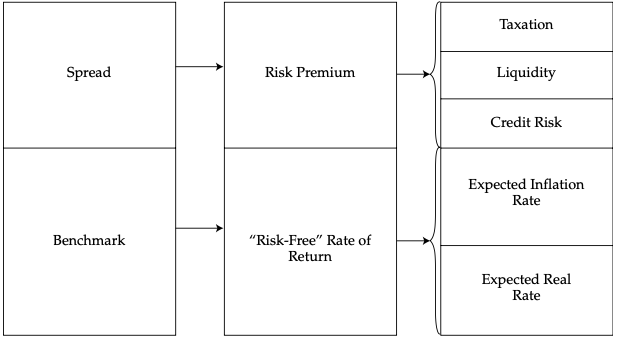
\includegraphics[scale=0.4]{/fi/yscom}
\caption{Components of Yield Spread}
\end{figure}

\begin{flushleft}
Summary of Yield Conventions
\begin{tabularx}{\textwidth}{p{11em}|X}
\hline
\rowcolor{gray!30}
Convention & Meaning \\
\hline
Actual$/$Actual & Actual number of days from prior coupon payment to settlement date/number of days in coupon period, assuming actual number of days in a year.\\
& Typically used with government bonds. \\
\hline
$30/360$ & Number of days from prior coupon payment to settlement date, assuming $30$ days in a month/number of days in a coupon period, assuming $360$ days in a year.\\
& Typically used with corporate bonds.\\
\hline
Street Convention & Yield measure that does not account for weekends and bank holidays and thus assumes cash flows are paid on their scheduled dates. \\
\hline
True Yield & Yield measure that accounts for weekends and bank holidays and thus assumes cash flows are paid after their scheduled dates. True yield is never higher than street convention yield due to the delay in time to payment.\\
\hline
Government Equiv Yield & Yield measure that restates a $30/360$ day count YTM to one based on an Actual$/$Actual day count. It is used to restate the YTM on a corporate bond to obtain the spread over the government YTM.\\
\hline
Simple Yield & Yield measure that is the sum of coupon payments plus the straight-line amortised share of the gain or loss, divided by the flat price.\\
& It is used mostly to quote Japanese government bonds (JGBs). \\
\hline
\end{tabularx}
\end{flushleft}

\begin{definition} \hlt{Annual Percentage Rate (APR)}\\
Allows conversion of an annualised yield in one periodicity to another periodicity. Compounding more frequently with lower annual rate corresponds to compounding less frequently at higher annual rate.
\begin{equation}
\left(1 + \frac{\text{APR}_m}{m} \right) = \left(1 + \frac{\text{APR}_n}{n} \right) \nonumber
\end{equation}
\end{definition}

\begin{definition} \hlt{Current Yield}\\
Measure equal to bond's annual coupon divided by flat price. Focuses solely on interest income, ignores frequency of coupon payments, interest on interest (time value of money), and accrued interest.
\begin{equation}
\text{CY}_t = \frac{\text{Annual Coupon}_t}{\text{Bond Price}_t} \nonumber
\end{equation}
\end{definition}

\begin{definition} \hlt{Simple Yield}\\
Used to quote Japanese government bonds (JGBs).
\begin{equation}
\text{Simple Yield} = \frac{1}{PV^{\text{Flat}}} \left(\sum PMT + \text{Straight Line Amortisation of Gain/Loss} \right) \nonumber
\end{equation}
\end{definition}

\begin{definition} \hlt{Bonds with Embedded Options: Yield-to-Call}\\
To modify return measure that takes bond's call feature into account.
\begin{align}
PV &= \sum\limits_{t=1}^N \frac{PMT}{(1+r)^t} + \frac{\text{Call Price}}{(1+r)^N} \nonumber \\
\text{Yield-to-Worst} &= \min\{r_i, YTM\} \nonumber
\end{align}
where $r$ is yield-to-call, to be separately calculated for each call date.\\
The \hlt{Option-Adjusted Price} is value of embedded call option added to flat price of bond. Investor bears call risk, hence embedded call option reduces value of.
\end{definition}

\begin{definition} \hlt{Option-Adjusted Yield}\\
Compute the value of the embedded option with the option pricing model, taking estimate of future interest rate volatility. Next, compute the option-adjusted price,
\begin{equation}
\text{Option-Adjusted Price} = PV^{\text{Flat}} + \text{Value of Option} \nonumber
\end{equation}
Lastly, use the option-adjusted price to compute for the yield.
\end{definition}

\begin{definition} \hlt{Bond Equivalent Yield (BEY)}\\
Periodic bond yields for straight, zero-coupon bonds computed based on semi-annual periods.\\
This yield is an internal rate of return with semi-annual compounding.
\begin{equation}
\text{BEY} = \frac{\text{Face Value} - \text{Price}}{\text{Price}} \times \frac{365}{\text{Days to Maturity}} \nonumber
\end{equation}
\end{definition}

\begin{definition} \hlt{Effective Annual Yield (EAY)}\\
Measure of return on bond if coupon payments reinvested.
\begin{equation}
\text{EAY} = \left(1 + \frac{r}{n} \right)^n - 1 \nonumber
\end{equation}
\end{definition}

\begin{remark} \hlt{BEY and EAY Relationship}\\
BEY is obtained with simple interest to annualise semi-annual YTM.
\begin{align}
\text{BEY} &= 2 \times \text{Semi-annual YTM} \nonumber \\
\text{EAY} &= \left(1 + \frac{\text{Semi-annual BEY}}{2} \right)^2 - 1 \nonumber \\
\text{BEY} &= 2(\sqrt{1+\text{EAY}} - 1) \nonumber 
\end{align}
\end{remark}

\begin{definition} Benchmark Rate Terminologies
\begin{enumerate}[label=\roman*.]
\setlength{\itemsep}{0pt}
\item On-the-Run Security: most recently issued government bond, which is also the most actively traded security and has coupon rate closest to current market discount rate. Price is close to par value.
\item Off-the-Run Security: seasoned government bonds, trade at slightly higher YTM than on-the-run bonds wth same or similar times-to-maturity, due to differences in demand for the securities and cost of financing.
\item Benchmark Spread; yield spread over a specific benchmark, represents credit risk premium, liquidity risk premium, and tax impact.
\end{enumerate}
\end{definition}

\begin{figure}[H]
\centering
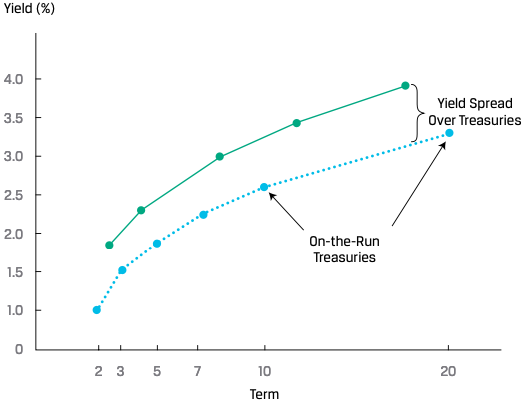
\includegraphics[scale=0.5]{/fi/otrvsotr}
\caption{On-the-run treasuries and seasoned treasuries}
\end{figure}

\begin{definition} \hlt{Government-Spread (G-Spread)}\\
Yield spread in basis points over an actual or interpolated government bond.\\
The return for bearing greater credit, liquidity, and other risks relative to the sovereign bond.
\end{definition}

\begin{method} \hlt{Approximation of G-Spread}\\
Used when comparable benchmark bond does not exist.
\begin{enumerate}[label=\roman*.]
\setlength{\itemsep}{0pt}
\item Compute the bond's current YTM
\item Linearly interpolate current rates (YTMs) for sovereign benchmark bonds with maturities closest to (below/above) given bond’s maturity, to find an approximate sovereign rate matching given bond’s maturity.
\item G-spread is difference between bond’s current YTM and interpolated sovereign benchmark rate.
\end{enumerate}
\end{method}

\begin{definition}
\label{def:ispread}
\hlt{Interpolated Spread (I-Spread)}\\
The yield spread for a bond over the standard swap rate in that currency of the same tenor.\\
Allows comparison of bonds with differing credit and liquidity risks against an interbank lending benchmark.\\
Issuers will use the I-spread to determine the relative cost of fixed-rate bonds versus floating-rate alternatives.\\
The higher the value of I-spread, the higher the compensation for liquidity and credit risk.
\end{definition}

\begin{definition} 
\label{def:zpsread}
\hlt{Zero-Volatility Spread (Z-Spread)}\\
Spread added to each benchmark spot rate to make the present value of a bond’s cash flows equal its price.
\begin{align}
PV = \sum\limits_{t=1}^N \frac{PMT}{(1 + z_t + Z)^t} + \frac{FV}{(1 + z_t + Z)^N} \nonumber
\end{align}
The benchmark spot or zero rates ($z_t$) are derived from government yield curve, or from fixed rates on interest rate swaps. $Z$ is the Z-spread.
\end{definition}

\begin{definition} \hlt{Option-Adjusted Spread (OAS)}\\
Spread of fixed-income security rate and risk-free rate of return, adjusted to take into account an embedded option. Based on an option-pricing model and an assumption about future interest rate volatility.
\begin{equation}
\text{OAS} = \text{Z-Spread} - \text{Option value in basis point per year} \nonumber
\end{equation}
For callable bonds, OAS $<$ Z-Spread.
\end{definition}

\begin{flushleft}
Summary of Yield Spreads
\begin{tabularx}{\textwidth}{p{11em}|X}
\hline
\rowcolor{gray!30}
Type & Description \\
\hline
G-Spread & Yield spread in basis points over an actual or interpolated government bond.\\
& Used in the US, the UK, Japan, and other jurisdictions. \\
\hline
I-Spread & Yield spread of a bond over the standard swap rate in the same currency and with the same tenor. Euro-denominated corporate bonds are typically priced vs. a euro interest rate swap benchmark. \\
\hline
Z-Spread & A constant yield spread over a government (or interest rate swap) spot curve used to derive the term structure of credit spreads for an issuer. \\
\hline
OAS & The Z-spread adjusted for the value of an embedded call option. \\
\hline
\end{tabularx}
\end{flushleft}

\subsubsection{Yield and Yield-Spread Measures for Floating-Rate Instruments}

\begin{remark} \hlt{Floating Rate Notes Characteristics}\\
Price is constant. Principal is non-amortising and redeemed in full at maturity.\\
Reference rate determined at beginning of period, and interest payment made at end of the period (‘in arrears’).
\end{remark}

\begin{remark} \hlt{Floating Rate Notes Coupons}\\
Fluctuates as interest rates change (tied to short-term money market rate, i.e. 3 month LIBOR).\\
Coupon is dependent on reference rate and quoted margin (spread), where spread is credit related.
\end{remark}

\begin{definition} Margin Terminology
\begin{enumerate}[label=\roman*.]
\setlength{\itemsep}{0pt}
\item \hlt{Quoted Margin}: to compensate investor for differences in credit risk of issuer and that implied by reference rate. Firms with very low credit risk may be able to obtain negative quoted margin.
\item \hlt{Required Margin}: yield spread over or under reference rate such that the FRN is priced at par value on a rate reset date. This is determined by market.\\
If quoted margin equals required margin at payment date, FRN is at par.\\
If FRN is priced in between payment dates, accrued interests are quoted on Actual$/360$ or Actual$/365$.
\end{enumerate}
\end{definition}

\begin{remark} \hlt{Changes in Required Margin of Floating Rate Notes}\\
Changes in required margin come from changes in issuer’s credit risk, liquidity or tax status.\\
If credit risk dropped, then quoted margin $<$ required margin, $PV > 100$ on payment date. FRN is premium.\\
If credit risk increased, then quoted margin $<$ required margin, $PV < 100$ on payment date. FRN is discount.
\end{remark}

\begin{remark} \hlt{FRN Pull-to-Par}\\
Between payment dates, flat price will be at premium (discount) to par value if reference rate goes down (up).\\
If required margin continues to be the same as quoted margin, the flat price is pulled to par value as next reset date nears.
At reset date, any change in reference date is included in interest payment for next period.
\end{remark}

\begin{definition} \hlt{Floating Rate Notes Pricing Model}
\begin{equation}
PV = \sum\limits_{t=1}^N \frac{\frac{(MRR + QM) \times FV}{m}}{\left(1 + \frac{MRR + DM}{m} \right)^t} + \frac{FV}{\left(1 + \frac{MRR + DM}{m} \right)^N} \nonumber
\end{equation}
where $MRR$ is the market reference rate, $QM$ is quoted margin, $m$ is periodicity of floating-rate note, $DM$ is discount margin (required margin), $N$ is number of periods to maturity. Model assumes the following:
\begin{enumerate}[label=\roman*.]
\setlength{\itemsep}{0pt}
\item The $PV$ is as of rate reset date; there is no accrued interest, so the flat price is full price.
\item $30/360$ day-count convention is used, but in practice Actual$/360$ day-count is used.
\item The same $MRR$ is used for all cash flows
\end{enumerate}
\end{definition}

\subsubsection{Yield and Yield-Spread Measures for Money-Market Instruments}

\begin{remark} \hlt{Differences in Yield Measures for Money Market vs Bonds}
\begin{enumerate}[label=\roman*.]
\setlength{\itemsep}{0pt}
\item Bond YTM are annualised and compounded. Money market yields are annualised but not compounded; the return on a money market instrument is stated on a simple interest basis.
\item Bond YTM are stated on a common periodicity for all times-to-maturity. Money market instruments with different times-to-maturity have different periodicities for the annual rate.
\item Bond YTM can be calculated using standard time-value-of-money analysis. Money market instruments are often quoted using non-standard interest rates and require different pricing equations.
\end{enumerate}
\end{remark}

\begin{method} \hlt{Discount-Rate Pricing}
\begin{equation}
PV = FV \times \left(1 - \frac{\text{Days}}{\text{Years}}\times DR \right) \nonumber
\end{equation}
where $DR$ is the discount rate stated in annual percentage rate. Equation may be rewritten as
\begin{equation}
DR = \frac{\text{Days}}{\text{Years}} \times \frac{(FV-PV)}{FV} \nonumber
\end{equation}
where the first term is periodicity of the annual rate. Note that the discount rate understates rate of return to investor, and understates cost of borrowed funds to issuer.\\
The quoted amount is $FV$, for commercial paper, treasury bills, banker's acceptances.
\end{method}

\begin{method} \hlt{Add-On Rate Pricing}
\begin{equation}
PV = \frac{FV}{\left( 1 +  \frac{\text{Days}}{\text{Years}} \times AOR \right)} \nonumber
\end{equation}
where $AOR$ is the add-on-rate in annual percentage term. Equation may be rewritten as
\begin{equation}
AOR = \frac{\text{Days}}{\text{Years}} \times \frac{(FV-PV)}{PV} \nonumber 
\end{equation}
First term is the periodicity, and second term is return on investment.\\
The quoted amount is $PV$, for bank certificates of deposit, repurchase agreements (Repos), MRRs.
\end{method}

\begin{method} \hlt{Comparing Money Market Instruments on Bond Equivalent Yield Basis}
\begin{enumerate}[label=\roman*.]
\setlength{\itemsep}{0pt}
\item For a MM instrument quoted on DR basis, determine price per 100 of Par (PV).
\item Determine AOR for this MM instrument using PV.
\item Bond Equivalent Yield (BEY) is a MM rate stated on a $365$-day AOR basis. This instrument is now comparable with other MM instruments expressed on a BEY basis.
\end{enumerate}
\end{method}

\subsubsection{Arbitrage-Free Valuation Framework}

\begin{definition} \hlt{Value Additivity Arbitrage}\\
Value of the whole differs from the sum of value of parts.
\begin{enumerate}[label=\roman*.]
\setlength{\itemsep}{0pt}
\item Stripping: portfolio of strips trading less than intact bond. To purchase the strips, combine them, then sell them as a bond.
\item Reconstitution: bond is worth less than its components. To purchase the bond, break it into portfolio of strips, then sell the components.
\end{enumerate}
\end{definition}

\begin{definition} \hlt{Dominance Arbitrage}\\
One asset trades at lower price than another asset with identical characteristics.
\end{definition}

\begin{figure}[H]
\centering
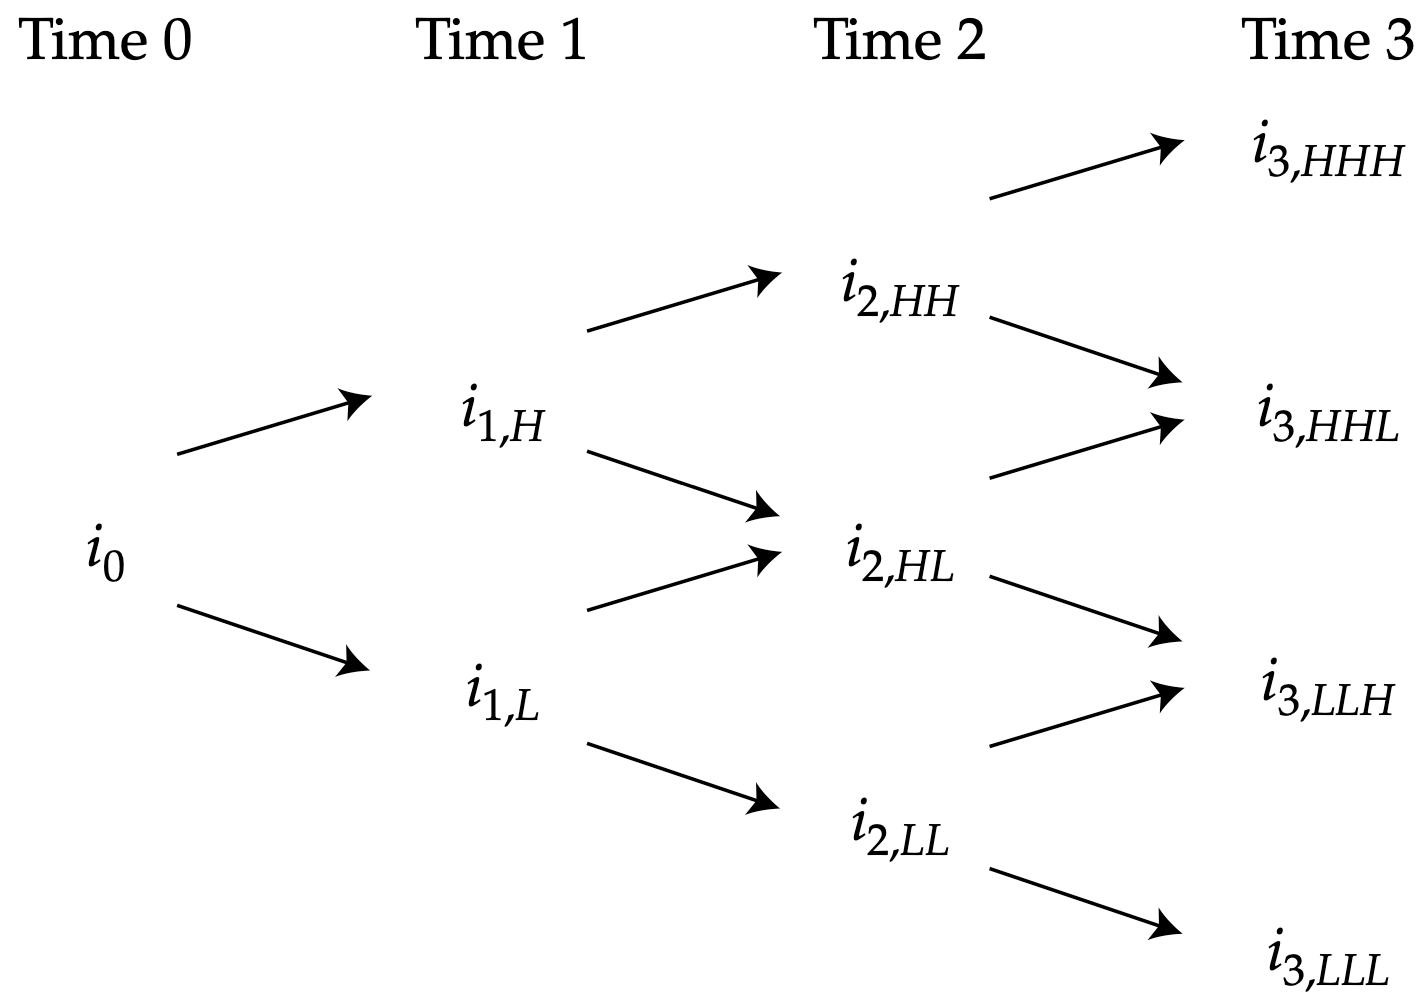
\includegraphics[scale=0.25]{/fi/bintree}
\caption{Binomial interest rate tree}
\end{figure}

\begin{method} \hlt{Binomial Interest Rate Tree}\\
Assumes interest rates have equal probability of taking one of two possible values in the next period.\\
Starting point $i_0$ of tree is current $1$-period spot rate.\\
A lognormal random walk is assumed for the implied interest rate, as lognormal properties allows for non-negativity of interest rates and higher volatility at higher interest rates. Note that
\begin{equation}
i_{1, H} = i_{i,L} e^{2 \sigma} \nonumber
\end{equation}
where $\sigma$ is the standard deviation of interest rates. Two vertical-adjacent nodes differ by factor of $e^{2 \sigma}$.
\end{method}

\begin{figure}[H]
\centering
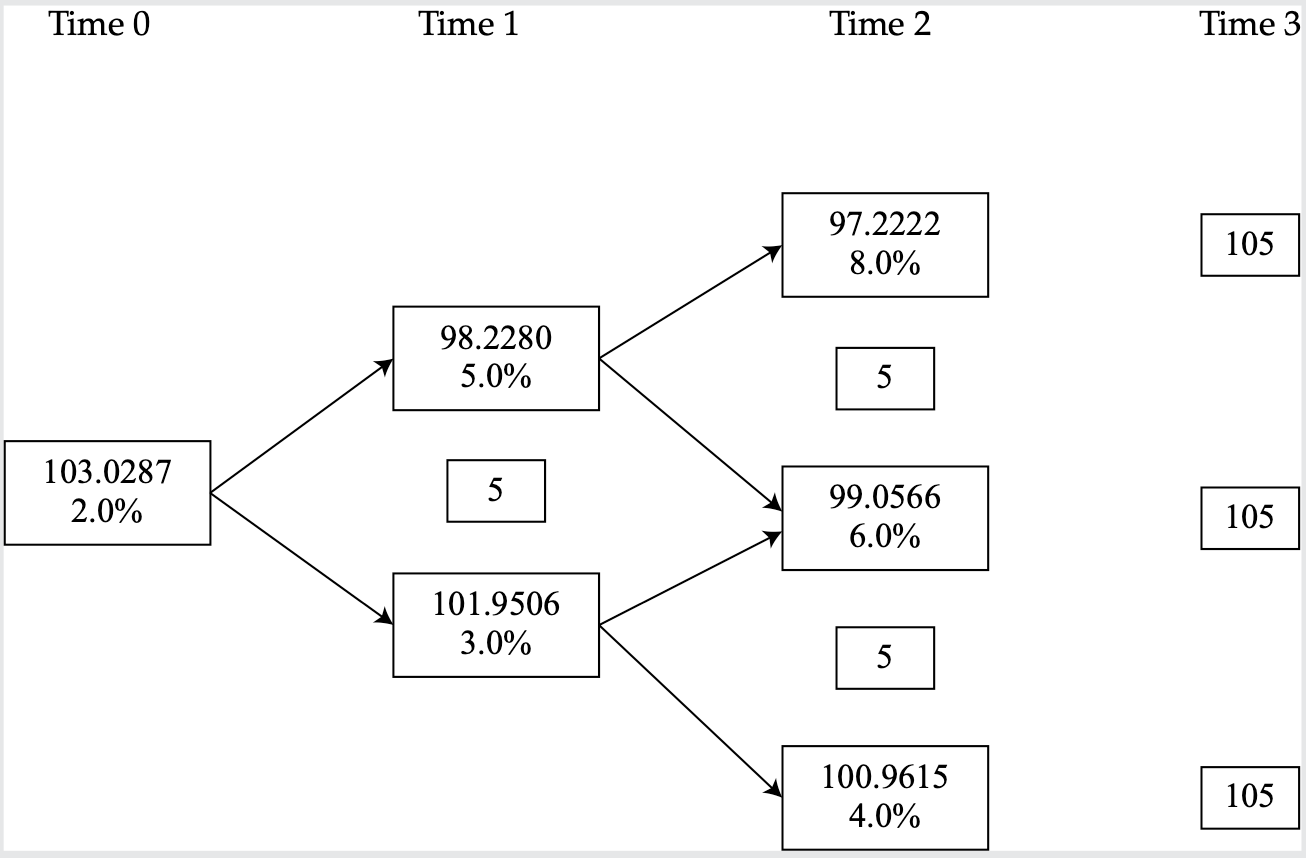
\includegraphics[scale=0.4]{/fi/backwardinduc}
\caption{Backward induction of binomial tree}
\end{figure}

\begin{method} \hlt{Backward Induction of Binomial Tree for Straight Bonds}\\
for $t$ in range $(0, T-1, -1)$: \# Computing from second last layer to the first \\
{\color{white}space} for $n$ in layer$\_t\_$nodes:
\begin{equation}
\text{v}(t,n) = \frac{\text{PMT}(t+1,n)+ [0.5 \text{v}(t+1, nH) + 0.5 \text{v}(t+1, nL)]}{1 + i(t, n)} \nonumber
\end{equation}
where $\text{v}(t,n)$ is value of node at time $t$ at position $n$, $\text{v}(t+1,nH)$ and $\text{v}(t+1,nL)$ is value of node at next time step $t+1$ at positions up ($H$) and down ($L$), $\text{PMT}(t+1,n)$ is beginning coupon payment for next time step, $i(t,n)$ is interest rate at time $t$ at position $n$ in decimal. \\
Note that at last layer $T$, the value at node $n$ is as follows:
\begin{equation}
\text{v}(T, n) = \frac{\text{PMT}(T,n) + \text{Redemption Value}(T,n)}{1 + i(T, n)} \nonumber
\end{equation}
\end{method}

\begin{remark} \hlt{Calibration of Software for Binomial Tree}
\begin{enumerate}[label=\roman*.]
\setlength{\itemsep}{0pt}
\item Interest rate tree should generated arbitrage-free values for benchmark security. Value of bonds produced by tree much be equal to their market pice.
\item Vertically-adjacent rates are $e^{2 \sigma}$ values apart
\item The middle forward rate in a period is approximately equal to the implied (from benchmark spot rate curve) one-period forward rate for that period
\end{enumerate}
\end{remark}

\begin{method} \hlt{Path-Wise Valuation}
\begin{enumerate}[label=\roman*.]
\setlength{\itemsep}{0pt}
\item Specify list of all potential paths along the tree
\item Determine the present value of a bond along each potential path
\item Calculate the average across all possible paths.
\end{enumerate}
\end{method}

\begin{method} \hlt{Monte Carlo Simulation}
\begin{enumerate}[label=\roman*.]
\setlength{\itemsep}{0pt}
\item Simulate numerous paths of interest rates under a volatility assumption and probability distribution
\item Generate spot rates from the simulated interest rates
\item Calculate present value from the cash flow along each interest rate path
\item Take the average of the present value across all interest rate paths
\end{enumerate}
Simulated paths should be calibrated so benchmark interest rate paths value benchmark securities at market price (arbitrage-free valuation). Calibration process involves adding/subtracting a constant to all rates when value from simulated paths is too high/low relative to market prices. This will result in a drift adjusted model.\\
Upper and lower bounds on interest rates may be imposed; bounds are based on notion of mean reversion.
\end{method}

\subsubsection{Valuation of Bonds with Embedded Options}

\begin{remark} \hlt{Embedded Options}\\
Allows issuer to manage interest rate risk, and/or issue bonds at an attractive coupon rate.
\end{remark}

\begin{remark} \hlt{Types of Bond Options}
\begin{enumerate}[label=\roman*.]
\setlength{\itemsep}{0pt}
\item Callable bond: gives issuer option to call back the bond. Investor is short the option.\\
Callable bonds usually have call protection period in which the bond cannot be called.
\item Putable bond: allows investor to put the bond back to issuer prior to maturity. Investor is long put.
\item Extendible bond: allows investor to extend maturity of bond.\\
May be evaluated as a putable bond with longer maturity.
\item Estate put: includes provision that allows heirs of investor to put the bond back to issuer upon death of investor. Value of contingent put option is inversely the investor's life expectancy.
\item Sinking fund bonds: require issuer to set aside funds periodically to retire the bond.\\
Reduces the credit risk of the bond over time. Sinkers typically have several related issuer options (call provisions, acceleration provisions, delivery options).
\end{enumerate}
\end{remark}

\begin{remark} \hlt{Value of Callable Bonds}\\
Investor is long bond but short the call option. Value of call option decreases the value of the callable bond.
\begin{equation}
v_{\text{Call Option}} = v_{\text{Straight Bond}} - v_{\text{Callable Bond}} \nonumber
\end{equation}
\end{remark}

\begin{remark} \hlt{Value of Putable Bonds}\\
Investor is long both bond and putable option. Value of put option increases the value of putable bond.
\begin{equation}
v_{\text{Put Option}} = v_{\text{Putable Bond}} - v_{\text{Straight Bond}} \nonumber
\end{equation}
\end{remark}

\begin{remark} \hlt{Interest Rate Volatility on Value of Callable or Putable Bond}\\
If interest rate volatility increases, values of both call and put options increase, hence value of callable bond decreases, while value of putable bond increases.
\end{remark}

\begin{figure}[H]
\centering
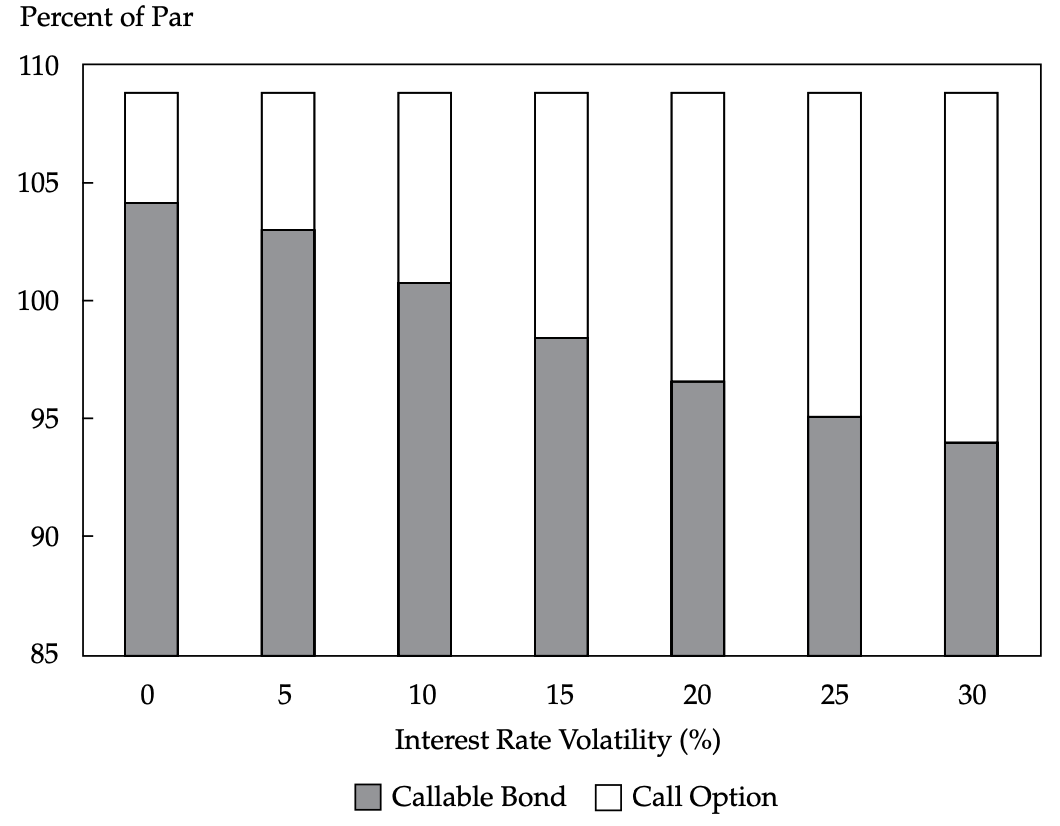
\includegraphics[scale=0.35]{/fi/volchangecallbond}
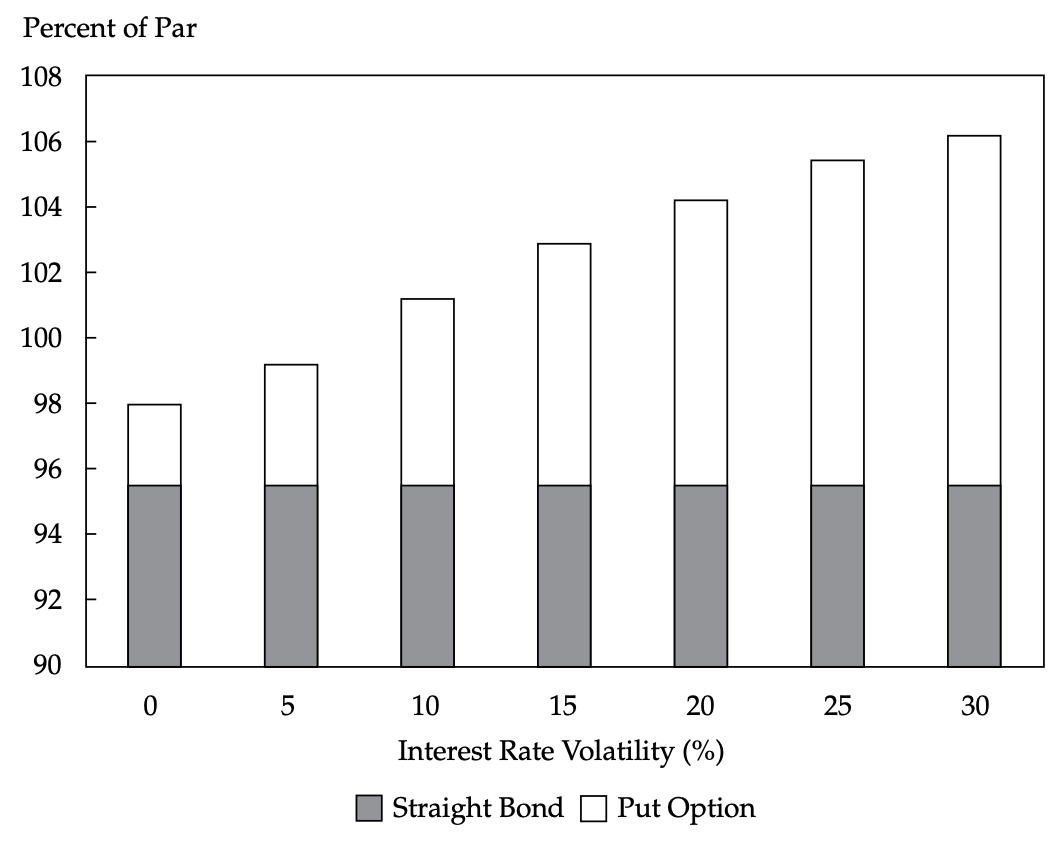
\includegraphics[scale=0.35]{/fi/volchangeputbond}
\caption{Effect of change in interest rate volatility on value of callable and putable bonds}
\end{figure}

\begin{remark} \hlt{Interest Rate Level on Value of Callable or Putable Bond}\\
As interest rates decrease, short call in callable bond limits bond's upside, hence value of callable bond rises less rapidly than value of otherwise equivalent straight bond.\\
As interest rtes increase, long put in putable bond hedges against loss in value, hence value of putable bond falls less rapidly than value of otherwise equivalent straight bond.\\
Call option value is inversely correlated to level of interest rates.\\
Put option is directly correlated to level of interest rates.
\end{remark}

\begin{figure}[H]
\centering
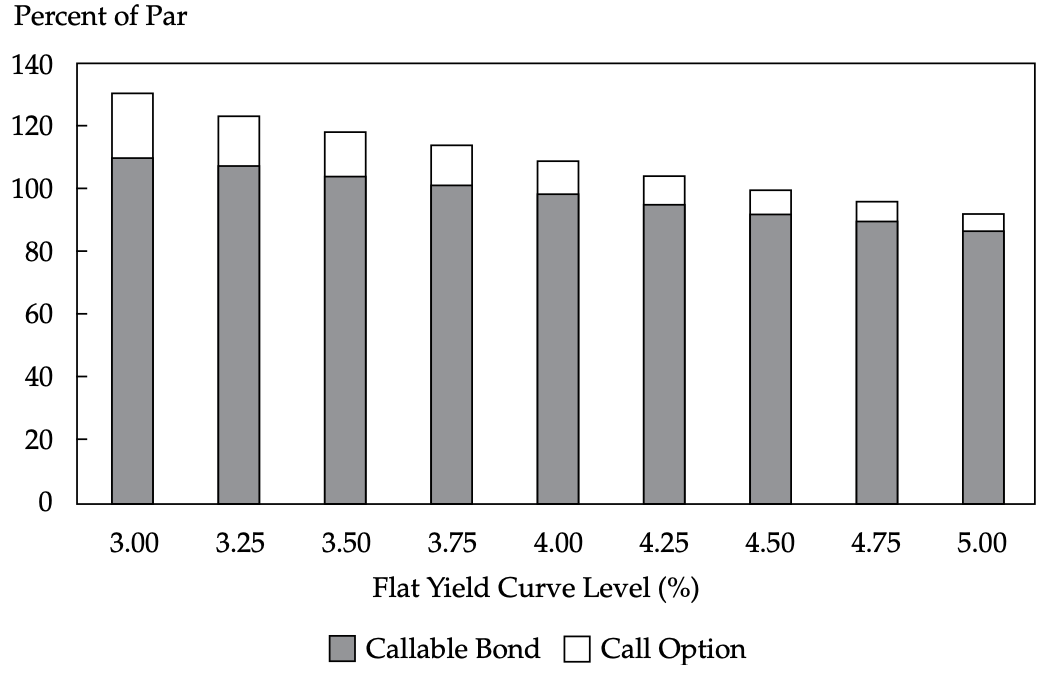
\includegraphics[scale=0.44]{/fi/flatyieldcurvelvcallbond}
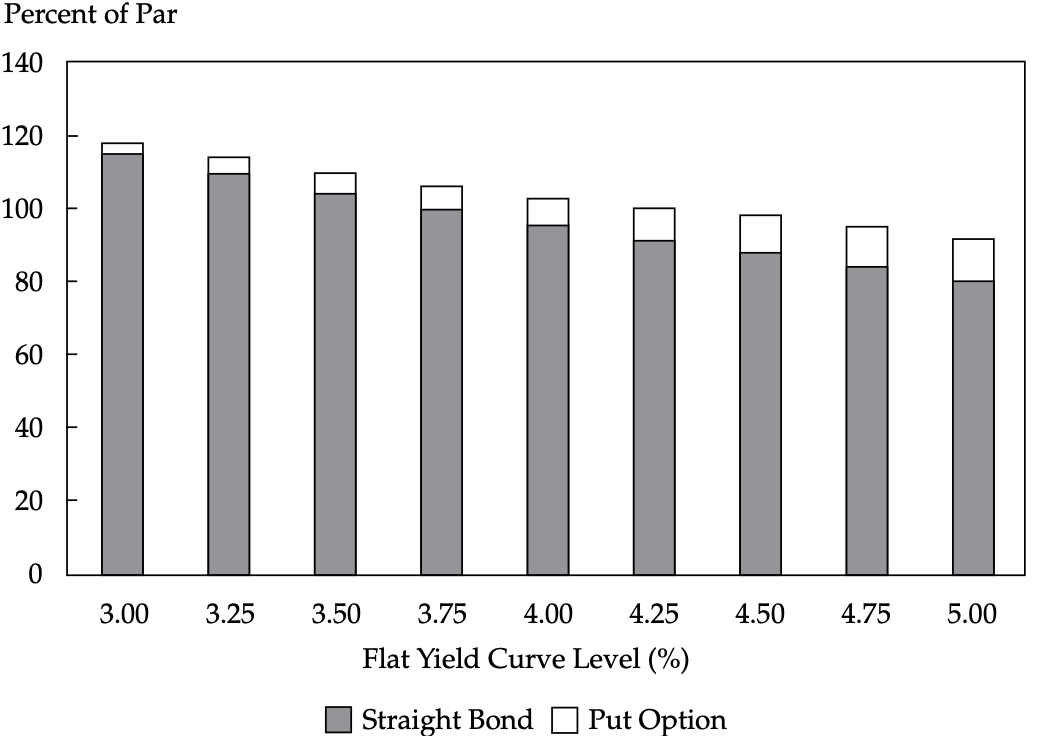
\includegraphics[scale=0.4]{/fi/flatyieldcurvelvputbond}
\caption{Value of callable and putable bond under different flat yield curve levels}
\end{figure}

\begin{remark} \hlt{Yield Curve Shape on Value of Callable or Putable Bond}\\
Value of embedded call option increases as interest rates decline.\\
When yield curve is upward sloping, distant one-period forward rates are higher than near one-period forward rates. Higher interest rate scenario limits probability of call option bing in the money, hence value of call option will be lower for upward sloping yield curve. As upward-sloping yield curve flattens, call option value increases.\\
Value of put option increases with interest rates. Upward sloping yield curve indicates higher probability of put option going in the money. Put option value declines as yield curve flattens.
\end{remark}

\begin{figure}[H]
\centering
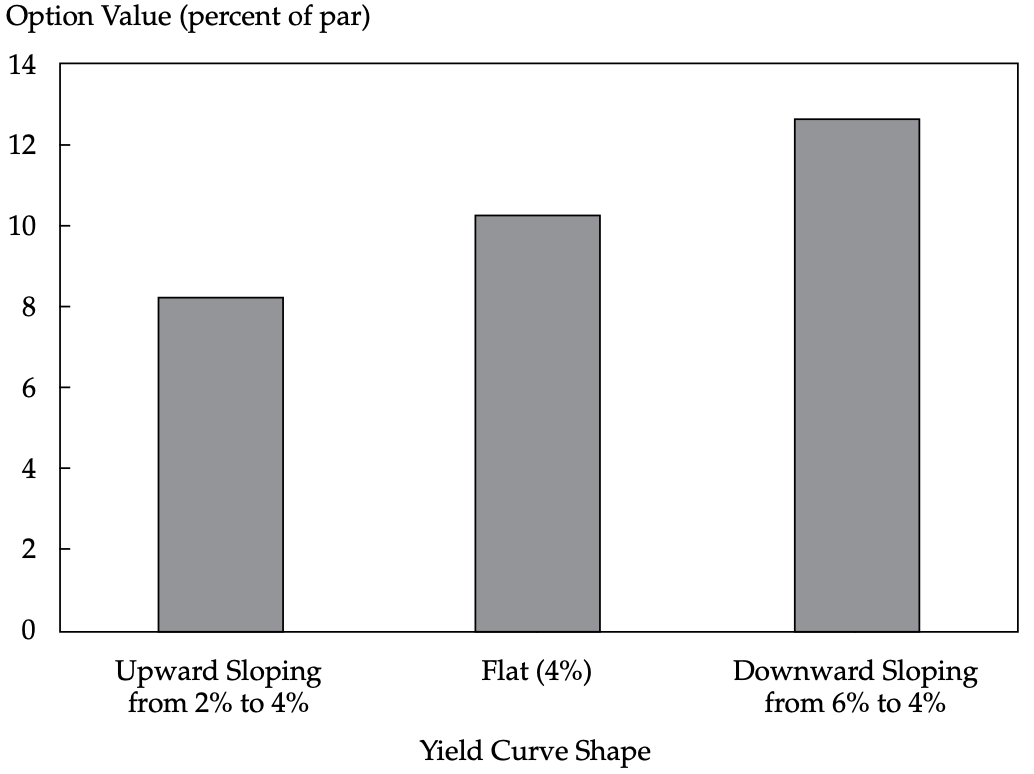
\includegraphics[scale=0.35]{/fi/yieldcurveshapecallbond}
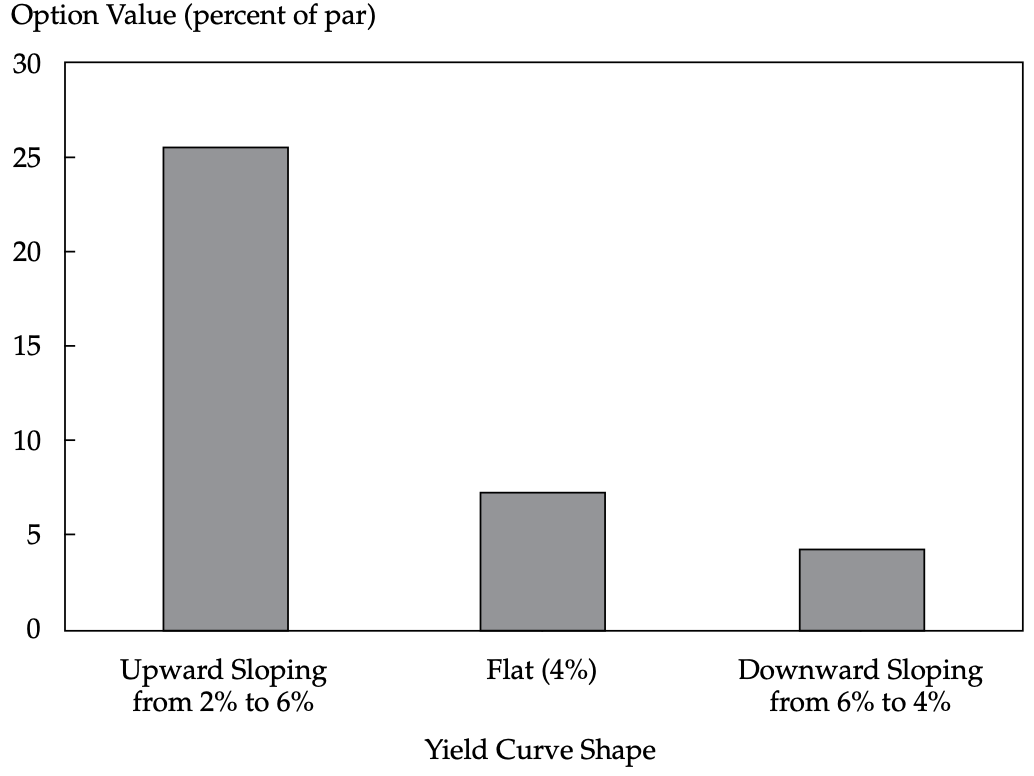
\includegraphics[scale=0.35]{/fi/yieldcurveshapeputbond}
\caption{Value of putable bond under different flat yield curve shapes}
\end{figure}

\begin{method} \hlt{Backward Induction of Binomial Tree for Bonds with Embedded Options}\\
One-period forward rates are used, instead of spot rates.
for $t$ in range $(0, T-1, -1)$: \# Computing from second last layer to the first \\
{\color{white}space} for $n$ in layer$\_t\_$nodes:
\begin{align}
\text{v}(t,n) = \frac{\text{PMT}(t+1,n)+ [0.5 \text{v}(t+1, nH) + 0.5 \text{v}(t+1, nL)]}{1 + i(t, n)} \nonumber
\end{align}
{\color{white}space} {\color{white}space} if option is callable:
\begin{equation}
\text{v}(t,n) = \min \{\text{Strike}, \text{v}(t,n) \} \nonumber
\end{equation}
{\color{white}space} {\color{white}space} if option is putable:
\begin{equation}
\text{v}(t,n) = \max \{\text{Strike}, \text{v}(t,n) \} \nonumber
\end{equation}
where $\text{v}(t,n)$ is value of node at time $t$ at position $n$, $\text{v}(t+1,nH)$ and $\text{v}(t+1,nL)$ is value of node at next time step $t+1$ at positions up ($H$) and down ($L$), $\text{PMT}(t+1,n)$ is beginning coupon payment for next time step, $i(t,n)$ is interest rate at time $t$ at position $n$ in decimal. \\
Note that at last layer $T$, the value at node $n$ is as follows:
\begin{equation}
\text{v}(T, n) = \frac{\text{PMT}(T,n) + \text{Redemption Value}(T,n)}{1 + i(T, n)} \nonumber
\end{equation}
\end{method}

\begin{figure}[H]
\centering
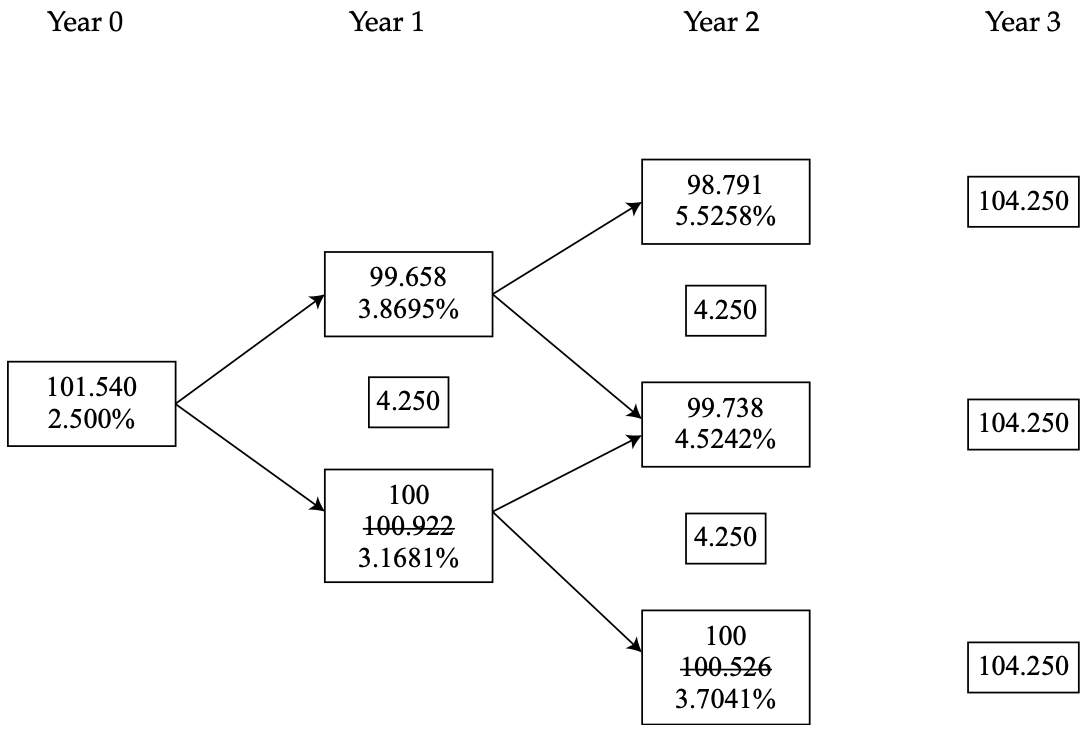
\includegraphics[scale=0.4]{/fi/backwardinduccallable}
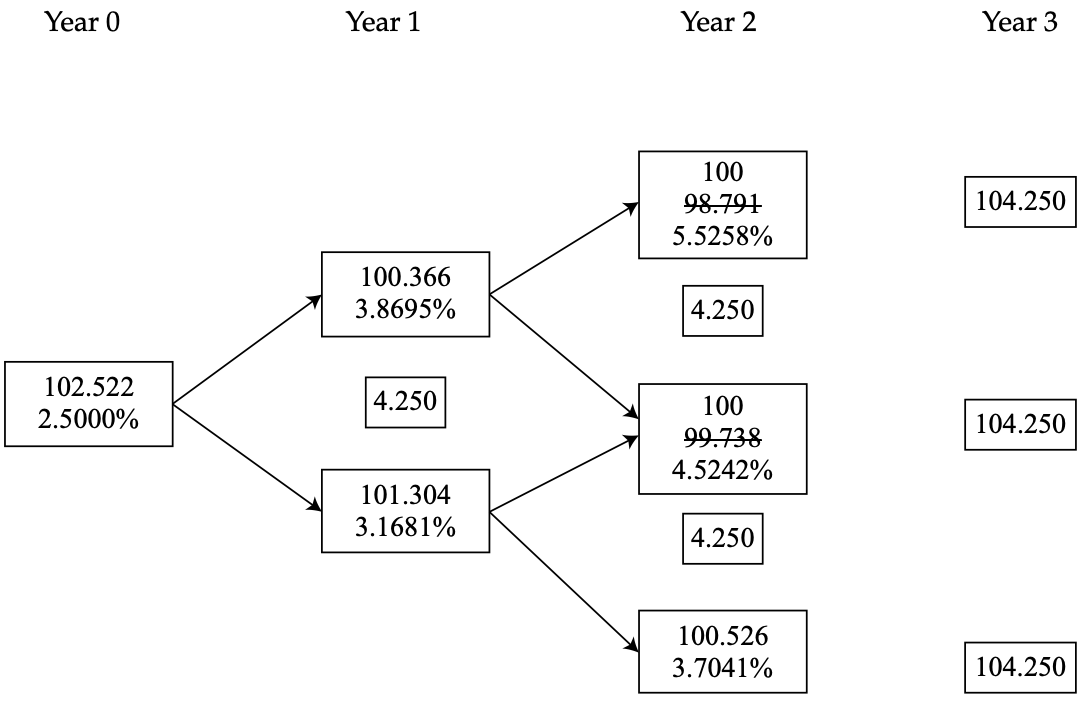
\includegraphics[scale=0.4]{/fi/backwardinducputable}
\caption{Backward induction with adjustment of node values for callable and putable bonds}
\end{figure}

\begin{remark} \hlt{Option-Adjusted Spreads (OAS) for Risky Callable and Putable Bonds}\\
Constant spread added to all one-period rates in the tree such that the calculated value equals market price. This spread is only added to the tree after adjustment for the embedded option.\\
If OAS for a bond is higher than OAS of its peers for the same credit risk, it is undervalued, vice versa.
\end{remark}

\begin{figure}[H]
\centering
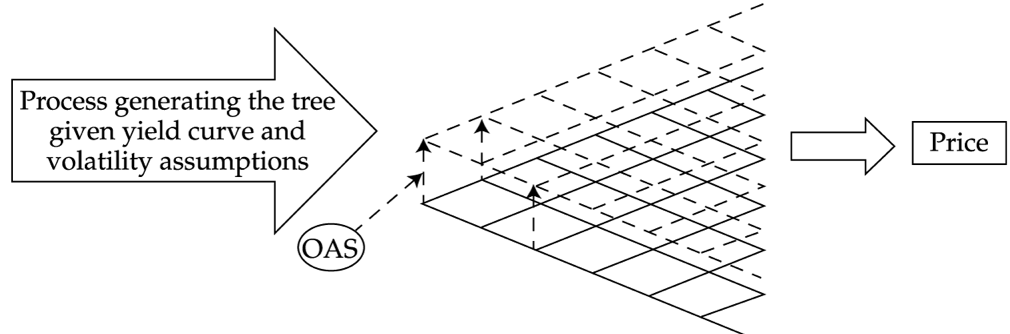
\includegraphics[scale=0.5]{/fi/oas}
\caption{Option-adjusted spread}
\end{figure}

\begin{remark} \hlt{Interest Rate Volatility on OAS}\\
Higher volatility lead to increased value of call option, hence decreasing the value of the call option. Hence when estimated volatility of benchmark rates used is higher, the computed value of callable bond will be lower, hence close to its true market price. The OAS that needs to be added to benchmark rates to correctly price the bond is therefore lower.\\
Hence, as assumed level of volatility used in interest rate tree increases, the computed OAS for a callable bond decreases. The computed OAS for a putable bond increases as the assumed level of volatility increases.
\end{remark}

\begin{flushleft}
Relationship Between Volatility and OAS
\begin{tabularx}{\textwidth}{p{5em}|X|X|X|X|X|X}
\hline
\rowcolor{gray!30}
Volatility & Call & Put & Callable & Putable & OAS$_{\text{Call}}$ & OAS$_{\text{Put}}$ \\
\hline
High & High & High & Low & High & Low & High \\
\hline
Low & Low & Low & High & Low & High & Low \\
\hline
\end{tabularx}
\end{flushleft}

\begin{figure}[H]
\centering
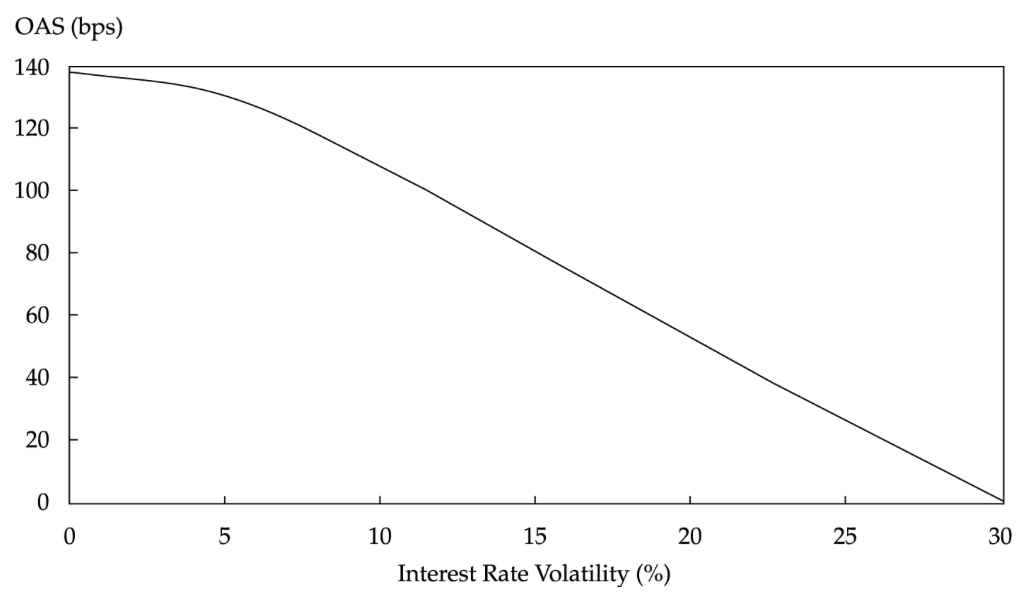
\includegraphics[scale=0.45]{/fi/voloas}
\caption{Interest rate volatility on OAS for a callable bond}
\end{figure}

\begin{remark} \hlt{Value of Floored Floater}\\
Capped floater protects investor against declining interest rates, hence is an investor option.\\
Investor is long bond long option, hence value of floor increases value of floored floater relative to straight bond.
\begin{equation}
v_{\text{Floored Floater}} = v_{\text{Straight Bond}} + v_{\text{Embedded Floor}} \nonumber
\end{equation}
\end{remark}

\begin{remark} \hlt{Value of Capped Floater}\\
Capped floater protects issuer against rising interest rates, hence is an issuer option.\\
Investor is long bond short option, hence value of cap decreases value of capped floater relative to straight bond.
\begin{equation}
v_{\text{Capped Floater}} = v_{\text{Straight Bond}} - v_{\text{Embedded Cap}} \nonumber
\end{equation}
\end{remark}

\begin{method} \hlt{Backward Induction of Binomial Tree for Floored Floater and Capped Floater}\\
One-period forward rates are used, instead of spot rates. \\
for $t$ in range $(0, T-1, -1)$: \# Computing from second last layer to the first \\
{\color{white}space} for $n$ in layer$\_t\_$nodes: \\
{\color{white}space} {\color{white}space} if option is floored floater:
\begin{equation}
\text{PMT}(t,n) = \min \{\text{Min Interest Rate} \times 100, \text{Coupon Rate} \times 100\} \nonumber
\end{equation}
{\color{white}space} {\color{white}space} if option is capped floater:
\begin{equation}
\text{PMT}(t,n) = \max \{\text{Min Interest Rate} \times 100, \text{Coupon Rate} \times 100\} \nonumber
\end{equation}
{\color{white}space} Then compute value:
\begin{align}
\text{v}(t,n) = \frac{\text{PMT}(t+1,n)+ [0.5 \text{v}(t+1, nH) + 0.5 \text{v}(t+1, nL)]}{1 + i(t, n)} \nonumber
\end{align}
where $\text{v}(t,n)$ is value of node at time $t$ at position $n$, $\text{v}(t+1,nH)$ and $\text{v}(t+1,nL)$ is value of node at next time step $t+1$ at positions up ($H$) and down ($L$), $\text{PMT}(t+1,n)$ is beginning coupon payment for next time step, $i(t,n)$ is interest rate at time $t$ at position $n$ in decimal. \\
Note that at last layer $T$, the value at node $n$ is as follows:
\begin{equation}
\text{v}(T, n) = \frac{\text{PMT}(T,n) + \text{Redemption Value}(T,n)}{1 + i(T, n)} \nonumber
\end{equation}
Redemption value to be computed using the floored or capped floater PMT computation earlier.
\end{method}

\begin{figure}[H]
\centering
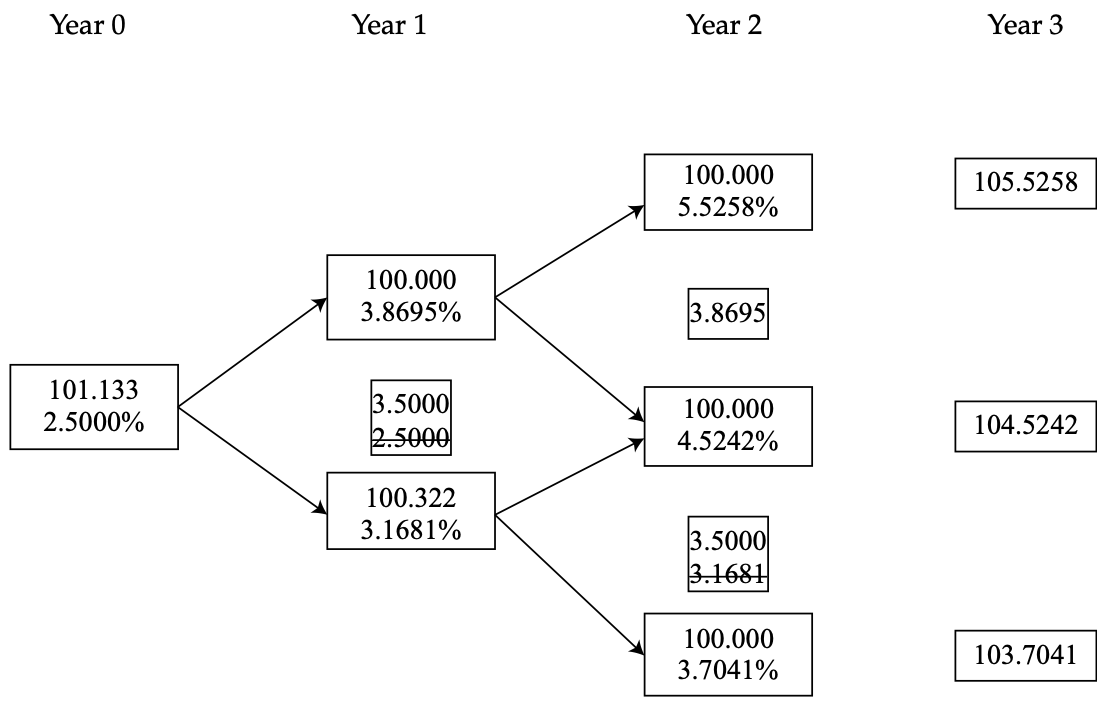
\includegraphics[scale=0.4]{/fi/backwardinducfloor}
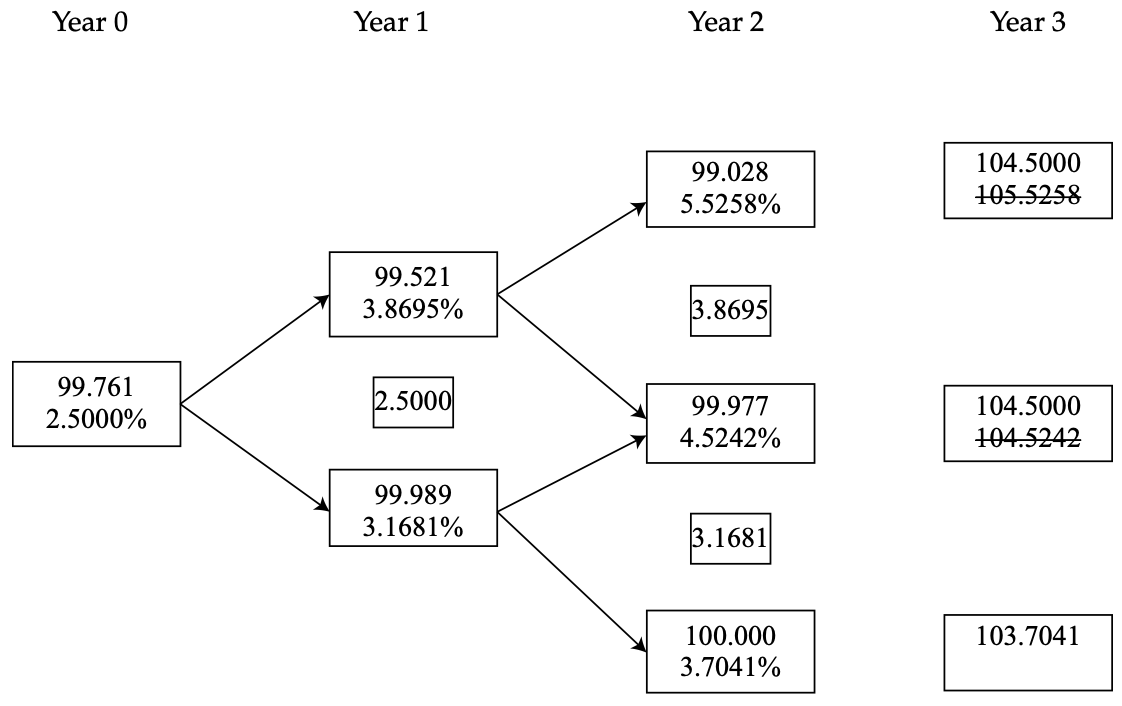
\includegraphics[scale=0.4]{/fi/backwardinduccap}
\caption{Backward induction with adjustment of node values for floor and cap floater bonds}
\end{figure}

\begin{remark} \hlt{Convertible Bonds}\\
Investor has right to convert the bond into fixed number of shares during the conversion period at conversion price, hence enjoying the upside of the issuer stock at cost of lower yield. Existing shareholders face dilution.\\
Offer document will indicate how the initial conversion ratio would be modified to account for corporate actions such as stock splits or stock dividends. \\
Offer documents may provide contingent put option in event of change-of-control events such as mergers; this may be exercised for a specific period of time after change of control. Alternatively, a lower conversion price may be specified in event of change of control. Conversion ratio may be adjusted upward if company pays dividend in excess of specified threshold dividend, hence protecting bondholders in event that the company pays out an unusually large dividend, which cause the ex-dividend price of stock to decline.\\
Other put options such as hard puts (i.e., redeemable for cash) or soft puts (i.e., issuer decides whether to redeem the bond for cash, stock, subordinated debentures, or combination of the three) may be embedded.
\end{remark}

\begin{remark} Convertible Bonds Terminology
\begin{enumerate}[label=\roman*.]
\setlength{\itemsep}{0pt}
\item \hlt{Conversion Value}: value of common stock that the bond maybe converted.
\begin{equation}
\text{Conversion Value} = \text{Market Price of Stock} \times \text{Conversion Ratio} \nonumber
\end{equation}
\item \hlt{Straight/Investment Value}: value of convertible bond if it were not convertible
\item \hlt{Minimum Value}: greater of its conversion value or straight value.\\
If convertible bond sells for less than its conversion value, then it could be purchased, immediately converted into common stock, and the stock sold for more than cost of the bond.
\item \hlt{Market Conversion Price/Conversion Parity Price}: price that convertible bondholder would pay for the stock if the bond is bought and immediately converted.
\begin{equation}
\text{Market Conversion Price} = \frac{\text{Market Price of Convertible Bond}}{\text{Conversion Ratio}} \nonumber
\end{equation}
\item \hlt{Market Conversion Premium Per Share}: market conversion price minus current market price.
\begin{equation}
\text{Market Conversion Premium Ratio} = \frac{\text{Market Conversion Premium per Share}}{\text{Market Price of Common Stock}} \nonumber
\end{equation}
\item \hlt{Premium Over Straight Value}: measure of downside risk, which is limited by bond's underlying straight value as price of convertible bond will not fall below this value.\\
The greater the premium over straight value, the less attractive the convertible bond.\\
Straight value is not constant, and varies with changes in interest rate and credit spread of bond.
\begin{equation}
\text{Premium Over Straight Value} = \frac{\text{Convertible Bond Price}}{\text{Straight Value}} - 1 \nonumber
\end{equation}
\end{enumerate}
\end{remark}

\begin{remark} \hlt{Contingent Convertibles}
\begin{enumerate}[label=\roman*.]
\setlength{\itemsep}{0pt}
\item Contingent Convertible Bonds ('CoCos'): pay higher coupon than otherwise identical non-convertible bonds, but are deeply subordinated and may be converted into equity or face principal write-downs if regulatory capital ratios are breached.
\item Convertible Contingent Convertible Bonds ('CoCoCos'): combined traditional convertible bond and a 'CoCo'. Convertible at discretion of investor, hence offering upside potential if share price increases. Also converted into equity or face principal write-downs in event of regulatory capital breach.
\end{enumerate}
\end{remark}

\begin{remark} \hlt{Value of Convertible Bonds in Arbitrage-Free Framework}\\
Investing in non-callable/non-putable convertible bond is equivalent to buying an option-free bond and a call option on amount of common stock equal to conversion ratio.
\begin{enumerate}[label=\roman*.]
\setlength{\itemsep}{0pt}
\item Non-Callable/Non-Putable Convertible Bond
\begin{equation}
\text{Bond Value} = \text{Straight Value} + \text{Call Option on Stock} \nonumber
\end{equation}
\item Callable Convertible Bond: includes call option that gives issuer right to call the bond
\begin{equation}
\text{Bond Value} = \text{Straight Value} + \text{Call Option on Stock} - \text{Call Option on Bond} \nonumber
\end{equation}
\item Convertible Bond that is Callable and Putable
\begin{equation}
\text{Bond Value} = \text{Straight Value} + \text{Call Option on Stock} - \text{Call Option on Bond} + \text{Put Option on Bond} \nonumber
\end{equation}
\end{enumerate}
\end{remark}

\begin{remark} \hlt{Difficulties of Valuing Convertible Bonds}\\
More difficult to value than callable bonds. To consider all of the factors that affect the value of callable bond, including interest rates and interest rate volatility, plus all of the factors that affect issuer’s common stock price and options on its common stock, such as its price volatility.
\end{remark}

\begin{remark} \hlt{Characteristics of Underlying Stock Price and Risk-Return of Convertible Bond}
\begin{enumerate}[label=\roman*.]
\setlength{\itemsep}{0pt}
\item If stock price falls, return on convertible bonds exceed those of the stock, as convertible bond's price has floor equal to straight bond value. As stock price approaches zero, convertible value will move towards the present value of estimated recovery.
\item If stock price rises, bond will underperform due to conversion premium.
\item If stock price is stable, return on convertible bond may exceed stock return due to coupon payments received from the bond, assuming no change in interest rates or credit risk of issuer.
\item If stock price is so low that it has little or no effect on convertible's price, bond trades as though it is a straight bond, and is referred to as a busted convertible.
\item If stock price is so high that convertible behaves as though it is an equity, the convertible is a common stock equivalent.
\end{enumerate}
\end{remark}

\begin{figure}[H]
\centering
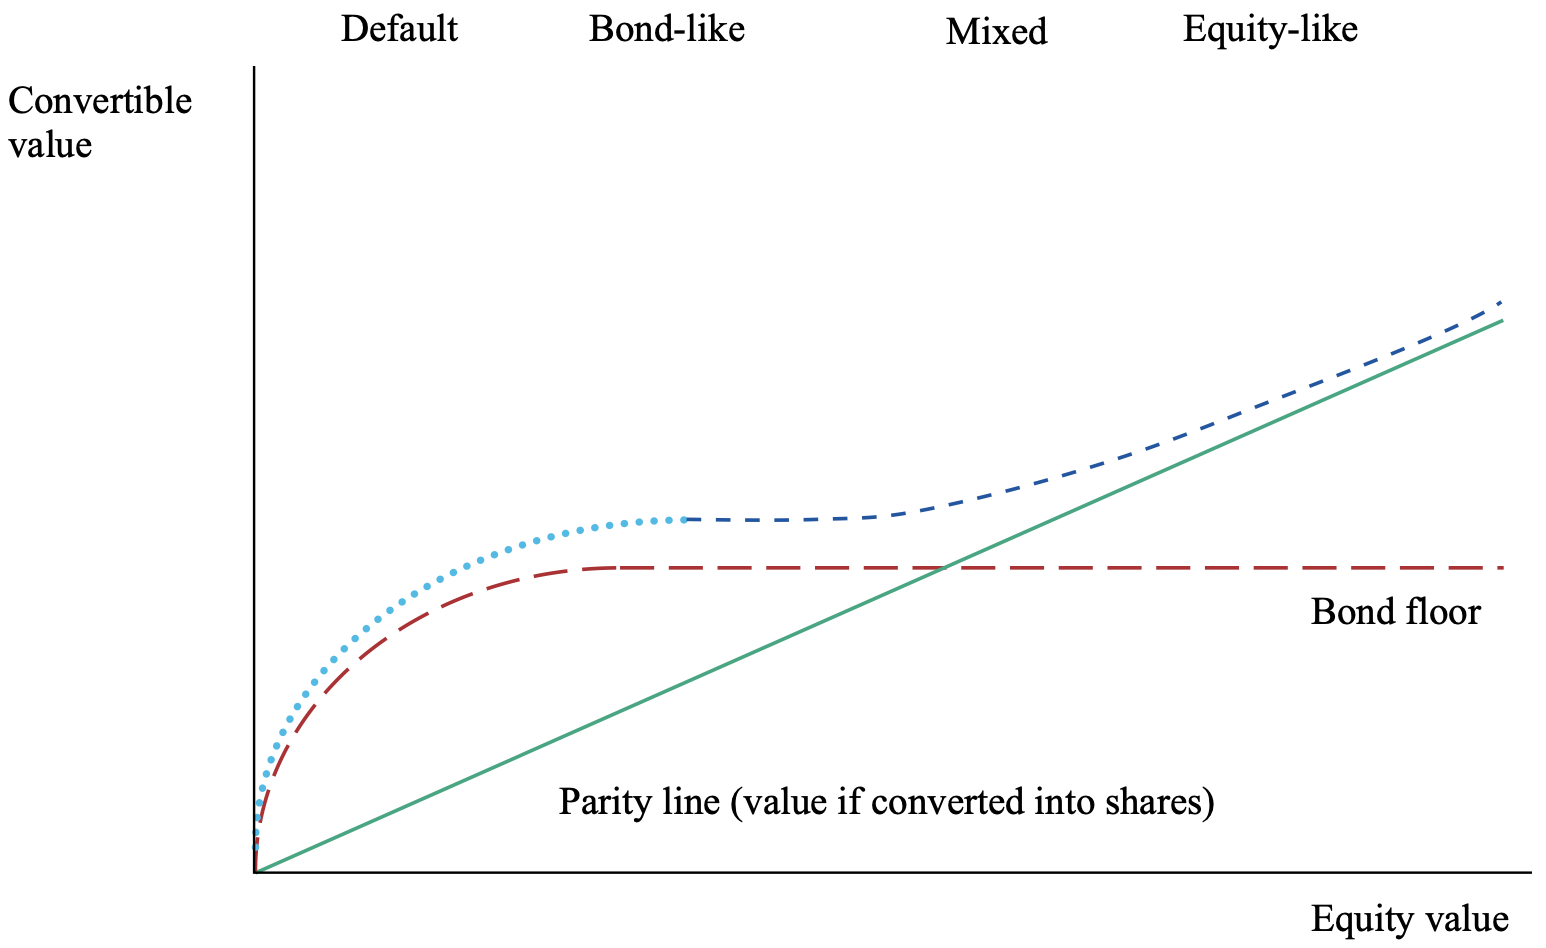
\includegraphics[scale=0.5]{/fi/convertiblebehavior}
\caption{Price behaviour of convertible bond and underlying common stock}
\end{figure}

\newpage

\subsection{Asset Backed Securities}



\newpage

\subsection{Fixed Income Risk}

\begin{remark} \hlt{Sources of Return in Fixed-Rate Bond}
\begin{enumerate}[label=\roman*.]
\setlength{\itemsep}{0pt}
\item Coupon and principal payments
\item Interest earned on coupon payments that are reinvested over holding period
\item Capital gain or loss if bond is sold before maturity
\end{enumerate}
\end{remark}

\begin{remark} \hlt{Performance of Return}\\
Assuming no credit risk, and the interest rate earned on reinvested coupon payments is the same as prevailing YTM on the bond, there are five key results:
\begin{enumerate}[label=\roman*.]
\setlength{\itemsep}{0pt}
\item Unchanged YTM, bond held to maturity: investor will earn annualised rate of return equal to YTM of the bond when purchased
\item Unchanged YTM, bond sold before maturity: investor will earn YTM of the bond
\item Changed YTM, bond held to maturity: if rates increase after the bond is purchased before first coupon date, holding a bond to maturity will earn rate of return greater than YTM at purchase
\item Changed YTM, bond sold before maturity in short period: if rates increases after bond is purchased before first coupon date, investor will earn lower than YTM at purchase
\item Changed YTM, bond sold before maturity in long period: if rates decreases after bond is purchased before first coupon date, investor will earn lower than YTM at purchase
\end{enumerate}
\end{remark}

\begin{definition} \hlt{Price Risk}\\
The uncertainty on bond's price due to uncertainty about prevailing market YTM at time of sale
\end{definition}

\begin{definition} \hlt{Reinvestment Risk}\\
The uncertainty about total coupon payments and reinvestment income on these payments due to uncertainty about future reinvestment rates.
\end{definition}

\begin{remark} \hlt{Price Risk vs Reinvestment Risk}
\begin{enumerate}[label=\roman*.]
\setlength{\itemsep}{0pt}
\item Short investment time horizon: price risk > reinvestment risk
\item Long investment time horizon: price risk < reinvestment risk
\end{enumerate}
Premium bond is more dependent on reinvestment income than par bond.\\
Zero-coupon bonds has no reinvestment risk if held to maturity as there is no periodic cash flow to be reinvested.
\end{remark}

\subsubsection{Yield-Based Duration and Convexity Measures}

\begin{definition} \hlt{Bond Duration}\\
Measures sensitivity of bond’s full price to changes in bond’s own yield, or to changes in benchmark rate.\\
Represents approximate amount of time a bond to be held for market discount rate to be realised.
\end{definition}

\begin{definition} \hlt{Yield Duration}\\
Sensitivity of bond price to its own YTM.\\
May be Macaulay, Modified, Money, Price Value of a Basis Point (PVBP)
\end{definition}

\begin{definition} \hlt{Curve Duration}\\
Sensitivity of price to benchmark yield, as measured by effective duration.\\
Change in benchmark yield not equal same change in bonds YTM, to be measured based on par curve.
\end{definition}

\begin{definition} \hlt{Portfolio Duration}\\
Weighted average of duration of individual bonds in portfolio.\\
Can be used for bonds with embedded options. However, using cash flow yield is theoretical correct.
\end{definition}

\begin{definition} \hlt{Macaulay Duration Long Form}
\begin{equation}
\text{MacDur} = \frac{\sum\limits_{n=1}^N \frac{(n - t/T) \times PMT}{(1+r)^{n - t/T}} + \frac{(N - t/T) \times FV}{(1+r)^{N - t/T}}}{\sum\limits_{n=1}^N \frac{PMT}{(1+r)^{n - t/T}} + \frac{FV}{(1+r)^{N - t/T}}} \nonumber
\end{equation}
where $t$ is days from last coupon payment to settlement date, $T$ is number of days in coupon period, $PMT$ is coupon payment per period, $FV$ is future value paid at maturity or par value of bond, $r$ is YTM or market discount rate per period, $N$ is number of evenly spaced periods to maturity as of beginning of current period.\\
Note that the denominator is the full price of bond including accrued interest.
\begin{equation}
PV^{\text{Full}} = \sum\limits_{n=1}^N \frac{PMT}{(1+r)^{n - t/T}} + \frac{FV}{(1+r)^{N - t/T}} \nonumber
\end{equation}
\end{definition}

\begin{definition} \hlt{Macaulay Duration Closed Form}
\begin{equation}
\text{MacDur} = \left\{\frac{1+r}{r} - \frac{1+r+[N \times (c-r)]}{c \times [(1+r)^N - 1] + r} \right\} - \frac{t}{T} \nonumber
\end{equation}
where $c$ is coupon rate per period.
\end{definition}

\begin{definition} \hlt{Annualised Macaulay Duration}
\begin{equation}
\text{AnnMacDur} = \frac{\text{MacDur}}{\text{Number of coupon payments in a year}} \nonumber
\end{equation}
\end{definition}

\begin{flushleft}
\begin{tabularx}{\textwidth}{X|X|X}
\hline
\rowcolor{gray!30}
Scenario & Dominant Risk & Source of Interest Rate Risk \\
\hline
Investment Horizon $>$ MacDur & Reinvestment risk & Falling interest rates \\
\hline
Investment Horizon $=$ MacDur & Equal risk & $-$ \\
\hline
Investment Horizon $<$ MacDur & Price risk & Rising interest rates \\
\hline
\end{tabularx}
\end{flushleft}

\begin{figure}[H]
\centering
\includegraphics[scale=0.45]{/fi/macdurirrise}\hfill
\includegraphics[scale=0.45]{/fi/macdurirdrop}
\caption{Interest rate effects on Macaulay Duration}
\end{figure}

\begin{remark} \hlt{Interpretation of Macaulay Duration}\\
Weighted average of time to receipt of bond’s promised payments, where the weights are shares of full price that correspond to each of the bond’s promised future payments
\end{remark}

\begin{method} \hlt{Computing Macaulay Duration}
\begin{enumerate}[label=\roman*.]
\setlength{\itemsep}{0pt}
\item Calculate PV of each payment for each period
\item Calculate weight of each payment as percentage of total PV
\item Take the weighted of each payment, multiply by $(i-t/T)$
\item Sum up the results from above step to get MacDur.
\end{enumerate}
\end{method}

\begin{definition} \hlt{Modified Duration}\\
Provides an estimate of the percentage price change for a bond given a change in YTM (linear estimate).
\begin{equation}
\text{ModDur} = \frac{\text{MacDur}}{1+r} \nonumber
\end{equation}
Annualised modified duration may be computed by dividing by the number of coupon periods per year.
\begin{equation}
\text{AnnModDur} = \frac{\text{ModDur}}{\text{Number of coupon payments in a year}} \nonumber = \frac{\text{AnnMacDur}}{1+r} \nonumber
\end{equation}
\end{definition}

\begin{remark} \hlt{Annualised Modified Duration and Full Bond Price Relationship}
\begin{equation}
\%\Delta PV^{\text{Full}} \approx - \text{AnnModDur} \times \Delta \text{Annualised Yield} \nonumber
\end{equation}
If interest rate increase, price of bond decrease, and yield $>0$, thus $PV^{\text{Full}}$ decrease.
\end{remark}

\begin{remark} \hlt{Approximate Modified Duration}\\
If Macaulay Duration is not known, Modified Duration may be approximated.
\begin{align}
\text{AnnModDur} &\approx \frac{(PV_{-}) - (PV_{+})}{2 \times (\Delta \text{Yield}) \times PV_0} \nonumber \\
\text{AnnMacDur} &\approx \text{AnnModDur} \times (1+r) \nonumber
\end{align}
for a small $\Delta$Yield.
\end{remark}

\begin{figure}[H]
\centering
\includegraphics[scale=0.55]{/fi/moddurapprox}
\caption{Approximating modified duration}
\end{figure}

\begin{definition} \hlt{Money Duration}\\
A measure of the price change in currency units. The money duration can be stated per $100$ of par value or in terms of the actual position size.
\begin{align}
\text{MoneyDur} &= \text{AnnModDur} \times PV^{\text{Full}} \nonumber \\
\%\Delta PV^{\text{Full}} &\approx - \text{MoneyDur} \times \Delta \text{Yield} \nonumber
\end{align}
\end{definition}

\begin{definition} \hlt{Price Value of a Basis Point (PVBP)}\\
An estimate of the change in the full price of a bond given $1$ bp change in its yield-to-maturity.
\begin{equation}
\text{PVBP} = \frac{(PV_{-}) - (PV_{+})}{2} \nonumber
\end{equation}
\end{definition}

\begin{flushleft}
Summary of Yield-Based Duration Measures
\begin{tabularx}{\textwidth}{p{5em}|X|X}
\hline
\rowcolor{gray!30}
Measure & Calculation & Use \\
\hline
MacDur & Average time to receipt of promised cash flows, weighted by shares of the full price corresponding to each promised future cash flow & Holding period that would balance reinvestment and price risks\\
\hline
ModDur & First derivative of price with respect to yield. MacDur divided by $1 +$ yield per period & Estimate percentage price change for a bond given a change in its yield-to-maturity \\
\hline
MoneyDur & Modified duration multiplied by full price of bond or bond position & Estimate price change in bond investment for a given yield change \\
\hline
PVBP & Difference in price of a $1$ bp yield decrease and a $1$ bp yield increase, divided by $2$ & Estimate of the change in the bond price given a $1$ bp change in the yield-to-maturity \\
\hline
\end{tabularx}
\end{flushleft}

\begin{remark} Duration of Zero-Coupon Bond\\
As zero-coupon bonds have a single payments, face value at maturity, present weighted-average time to receipt of cash flows is same as time-to-maturity as that single cash flow has a present value weight of $1$.\\
Macaulay duration of a zero-coupon bond is its time-to-maturity, modified duration is time-to-maturity divided by $1$ plus yield.
\end{remark}

\begin{remark} Duration of Perpetual Bond\\
Bond does not mature, so there is no face or maturity value received at time $T$.\\
Non-callable perpetuities have Macaulay duration of $(1+r)/r$.
\end{remark}

\begin{remark} Duration of Floating-Rate Notes\\
Interest rate risk arises only between reset dates, as at the next reset date, coupon payments will adjust to the new MRR. Hence, the Macaulay duration for a floating-rate note or bond is simply the fraction of a period remaining until the next reset date, $(T-t)/T$.
\end{remark}

\begin{flushleft}
Properties of Yield Duration Statistics
\begin{tabularx}{\textwidth}{p{20em}|X}
\hline
\rowcolor{gray!30}
Increase in Feature & Effect on Duration (Interest Rate Risk) \\
\hline
Coupon rate $c$ & $\downarrow$ (inverse relationship) \\
\hline
Yield-to-maturity $r$ & $\downarrow$ (inverse relationship) \\
\hline
Time-to-maturity $T$ & $\uparrow$ (direct relationship) \\
\hline
Fraction of current coupon period elapsed $t/T$ & $\downarrow$ (inverse relationship) \\
\hline
\end{tabularx}
\end{flushleft}

\begin{figure}[H]
\centering
\includegraphics[scale=0.5]{/fi/macdurprop}
\caption{Properties of Macaulay Duration}
\end{figure}

\begin{definition} \hlt{Convexity}\\
Measures non-linear effect of yield changes on price for an option-free fixed-rate bond.\\
Fixed-rate bond will have greater convexity from:
\begin{enumerate}[label=\roman*.]
\setlength{\itemsep}{0pt}
\item longer time-to-maturity
\item lower coupon rate
\item lower yield-to-maturity
\item greater dispersion (degree to which payments are spread out over time)
\end{enumerate}
\end{definition}

\begin{figure}[H]
\centering
\includegraphics[scale=0.45]{/fi/convexity}
\caption{Convexity of an Option-Free Fixed-Rate Bond}
\end{figure}

\begin{remark} \hlt{Convexity Adjustment}
\begin{align}
\% \Delta PV^{\text{Full}} &\approx (-\text{AnnModDur} \times \Delta \text{Yield}) + \left[ \frac{1}{2} \times \text{AnnConvexity} \times (\Delta \text{Yield})^2 \right] \nonumber \\
\% \Delta PV^{\text{Full}} &\approx (-\text{MoneyDur} \times \Delta \text{Yield}) + \left[ \frac{1}{2} \times \text{MoneyConvexity} \times (\Delta \text{Yield})^2 \right] \nonumber
\end{align}
\end{remark}

\begin{flushleft}
Impact of changes in rates on duration and convexity
\begin{tabularx}{\textwidth}{p{10em}|X|X}
\hline
\rowcolor{gray!30}
Change in Rates & Impact on Duration & Impact on Convexity \\
\hline
$\Delta$BP $+$ & Negative & Positive \\
\hline
$\Delta$BP $-$ & Positive & Positive \\
\hline
\end{tabularx}
\end{flushleft}

\begin{definition} \hlt{Approximate Convexity}\\
Useful for bonds with uncertain cash flows, such as those with contingency features and default risk.
\begin{equation}
\text{ApproxConv} = \frac{(PV_{-}) + (PV_{+}) - [2 \times (PV_0)]}{(\Delta \text{Yield})^2 \times (PV_0)} \nonumber
\end{equation}
\end{definition}

\begin{figure}[H]
\centering
\includegraphics[scale=0.5]{/fi/convonoptfreebond}
\caption{Positive attributes of bond convexity on option-free bond}
\end{figure}

\begin{definition} \hlt{Exact Convexity}
\begin{equation}
\text{ExactConv} - \frac{[N - (t/T)] \times [N+1-(t/T)]}{(1+r)^2} \nonumber
\end{equation}
where $t/T$ is fraction of period that has passed, $r$ is YTM per period.
\end{definition}

\begin{remark} \hlt{Impact of Change in YTM on Convexity}\\
For two bonds with same price, YTM, and modified duration:\\
If YTM $\downarrow$, then the more convex bond will $\uparrow$ more in price.\\
If YTM $\uparrow$, then the more convex bond will $\downarrow$ less in price.\\
Hence, the more convex bond outperforms the less convex bond.\\
However, the more convex bond will have higher price, and lower YTM, hence investor have to pay for it.
\end{remark}

\begin{definition} \hlt{Weighted Average Time to Receipt of Aggregate Cash Flows}\\
Difficult in practice, as cash flow yield us not commonly calculated for bond portfolios.\\
Amount and timing of future cash payments are uncertain for bonds with embedded options or FRNs.\\
$\Delta$ cash flow yield is not the same as $\Delta$ YTM on individual bonds.\\
Interest rate risk is not usually expressed as $\Delta$ cash flow yield.
\end{definition}

\begin{definition} \hlt{Weighted Average Individual Bond Durations}\\
Easily used as measure of interest rate risk, i.e., $100$ bps rise in YTM, then estimated drop in portfolio is the average modified duration (AvgModDur).\\
Assumes parallel shift in yield curve. In reality, parallel shifts are rare.
\begin{align}
\text{AvgModDur} &= \sum\limits_{i=1}^N \text{ModDur}_i \left( \frac{\text{Bond}_{i, \text{Market Value}}}{\text{Portfolio Market Value}} \right) \nonumber \\
\text{ModDur}_i &= \frac{\text{AnnMacDur}_i}{1 + \frac{YTM_i}{m}} \nonumber
\end{align}
where $m$ is the periodicity.
\end{definition}

\subsubsection{Curve-Based and Empirical Duration and Convexity Measures}

\begin{definition} \hlt{Effective Duration}\\
Sensitivity of the bond’s price to a parallel change in a benchmark yield curve.
\begin{equation}
\text{EffDur} = \frac{(PV_{-}) - (PV_{+})}{2 \times \Delta \text{Curve} \times PV_0} \nonumber
\end{equation}
\end{definition}

\begin{definition} \hlt{Effective Convexity}
\begin{equation}
\text{EffConv} = \frac{(PV_{-}) + (PV_{+}) - [2 \times (PV_0)]}{(\Delta \text{Curve})^2 \times (PV_0)} \nonumber
\end{equation}
Callable bonds may have negative convexity (‘concavity’). Putable bonds always have positive convexity.
\end{definition}

\begin{figure}[H]
\centering
\includegraphics[scale=0.5]{/fi/callablebondrisk} \hfill
\includegraphics[scale=0.5]{/fi/putablebondrisk}
\caption{Interest rate risk characteristics of a callable bond and a putable bond}
\end{figure}

\begin{remark} \hlt{Effective Duration, Convexity Characteristics of Callable Bond}\\
Price of the non-callable bond is always greater than comparable callable bond; difference is embedded call option which is held by bond issuer.\\
When interest rates are high relative to coupon rate, value of call option is low.\\
When rates are low, the value of the call option is high since issuer is more likely to exercise the option to refinance debt at the lower prevailing rates.\\
Investor bears “call risk”. If the bond is called, investor must reinvest the proceeds at a lower interest rate.\\
When benchmark rates are high, effective duration of callable and non-callable bonds are very similar.\\
When benchmark rates are low, effective duration of callable bond is lower than comparable non-callable bond, as callable bond price does not increase as much when benchmark yields fall; call option limits price appreciation.
\end{remark}

\begin{remark} \hlt{Effective Duration, Convexity Characteristics of Putable Bond}\\
Price of putable bond is always higher than comparable non-putable bond; difference is embedded put option as held by investor.\\
Putable bond allows investor to sell bond back to issuer before maturity, usually at par value, protecting the investor from higher benchmark yields that would otherwise drive the bond’s price below par.\\
When benchmark rates are low, effective duration of putable and non-putable bonds are very similar.\\
When benchmark rates are high, put option is more valuable to investor, since the ability to sell the bond back to the issuer at par limits the price depreciation as rates rise.
\end{remark}

\begin{remark} \hlt{Relation to Full Price of Bond}
\begin{equation}
\% \Delta PV^{\text{Full}} \approx (-\text{EffDur} \times \Delta \text{Curve}) + \left[ \frac{1}{2} \times \text{EffConv} \times (\Delta \text{Curve})^2 \right] \nonumber
\end{equation}
\end{remark}

\begin{definition} \hlt{Key Rate Duration}\\
Measure of bond’s sensitivity to change in benchmark yield at a specific maturity (sensitivity to \hlt{shaping risk}).
\begin{align}
\text{KeyRateDur}_k &= - \frac{1}{PV} \times \frac{\Delta PV}{\Delta r_k} \nonumber \\
\text{EffDur} &= \sum\limits_{k=1}^n \text{KeyRateDur}_k \nonumber \\
\frac{\Delta PV}{\Delta r_k} &= -\text{KeyRateDur}_k \times \Delta r_k \nonumber
\end{align}
where $r_k$ represents the $k$th key rate.
\end{definition}

\begin{figure}[H]
\centering
\includegraphics[scale=0.5]{/fi/keyrateshiftone}
\includegraphics[scale=0.43]{/fi/keyrateshifttwo}
\caption{Key rate shift at single point, and across the benchmark curve}
\end{figure}

\begin{flushleft}
Summary of Curve-Based and Empirical Duration Statistics
\begin{tabularx}{\textwidth}{p{7em}|X|X}
\hline
\rowcolor{gray!30}
Measure & Definition & Interpretation \\
\hline
ApproxModDur & Estimates slope of line tangent to bond’s price–yield curve & Yield-based method to estimate ModDur \\
\hline
EffDur & Sensitivity of a bond’s price to a change in a benchmark yield curve & Curve-based method to estimate ModDur for complex bonds with uncertain cash flows \\
\hline
Key Rate & Measures bond sensitivity to benchmark yield change for a specific maturity & Partial duration statistic that gauges bond’s sensitivity to non-parallel benchmark yield curve changes \\
\hline
Empirical & Measure using historical data in statistical models and incorporating factors affecting bond prices to determine the price–yield relationship & Statistical estimate that accounts for correlation between yield spreads and benchmark yield-to-maturity changes under different economic scenarios \\
\hline
\end{tabularx}
\end{flushleft}

\newpage

\subsection{Term Structure and Interest Rate Dynamics}



\newpage

\subsection{Credit Analysis}

\begin{definition} \hlt{Credit Risk}\\
Risk associated with losses to fixed income investors, due to failure of borrower to make payment of interest or principal. When borrower fails to service their debt, they are in default.
\end{definition}

\subsection{Fundamentals of Credit Analysis}

\begin{figure}[H]
\centering
\includegraphics[scale=0.35]{/fi/csofcredit}
\caption{The Cs of Credit Analysis}
\end{figure}

\begin{remark} \hlt{Bottom-Up Credit Analysis Factors}
\begin{enumerate}[label=\roman*.]
\setlength{\itemsep}{0pt}
\item Capacity: measures borrower's ability to make debt payments on time
\item Capital: other resources available to borrower that reduce reliance on debt
\item Collateral: quality and value of assets supporting issuer's indebtedness
\item Covenants: legal terms and conditions the borrowers and lenders agree to as part of bond issue
\item Character: quality of management and willingness of repay indebtedness
\end{enumerate}
\end{remark}

\begin{remark} \hlt{Top-Down Credit Analysis Factors}
\begin{enumerate}[label=\roman*.]
\setlength{\itemsep}{0pt}
\item Conditions: general economic, competitive, and business environment faced by all borrowers that may affect their ability to service or refinance debt
\item Country: geopolitical environment, legal and political system faced by all issuers in a jurisdiction that may affect debt payment
\item Currency: affects issuers whose cash flows are affected by exchange rate changes or who borrow in a currency outside of their jurisdiction, such as sovereign issuers with foreign currency debt.
\end{enumerate}
\end{remark}

\begin{flushleft}
Borrower Types, Sources of Repayment, Sources of Credit Risk
\begin{tabularx}{\textwidth}{p{6.5em}|p{11em}|p{11em}|X}
\hline
\rowcolor{gray!30}
Borrower Type & Primary CF Source & Secondary CF Source & Credit Risk Source \\
\hline
Corporate & 
\xxx Business Operations
\xxx Investment, financing activities
&
\xxx Asset sales
\xxx Divestitures
\xxx Additional debt issuance
\xxx Equity issuance
&
\xxx Economic contraction
\xxx Strategic shifts in business and market environment
\xxx Increase competition
\xxx Reduced pricing power
\xxx Shrinking operating margin, increased losses
\xxx Excessive debt service needs \\
\hline
Soverigen or Public Entity & 
\xxx Taxes (income, sales, VAT, capital gains, wealth-based)
\xxx Tariffs, fees, other government revenue
&
\xxx Newly issued debt
\xxx Sale of public assets, privatisation
&
\xxx Economic contraction
\xxx Political uncertainty
\xxx Excessive debt service needs
\xxx Expansionary economic policies
\xxx Budget deficits
\xxx Tax cuts
\xxx Limited ability to collect taxes \\
\hline
\end{tabularx}
\end{flushleft}

\begin{figure}[H]
\centering
\includegraphics[scale=0.35]{/fi/sovcorpsourceofpayment}
\caption{Sovereign and Corporate Bond Sources of Repayment}
\end{figure}

\begin{remark} \hlt{Illiquid vs Insolvent}\\
Illiquid issuer is an issuer unable to raise cash to service debt.\\
Insolvent issuer has assets falling below the value of its debt.\\
An illiquid issuer may not necessarily be insolvent, but could still default.
\end{remark}

\begin{remark} \hlt{Bond Identure Clauses}
\begin{enumerate}[label=\roman*.]
\setlength{\itemsep}{0pt}
\item Cross-Default Clause: a default on one bond issuer causes a default on all issues
\item Pari Passu Clause: all bonds of certain type rank equally in the default process
\end{enumerate}
If both provisions exist on unsecured debt, a default on one issuer implies all holders of unsecured claims have access to general assets of the issuer to satisfy their obligations.\\
If both provisions exist on secured debt, default on any obligation of the issuer will grant access to general assets of the company and to assets pledged as collateral for the debt.\\
If value of pledged assets fall below amount of pari passu secured debt, secured bond investor have credit losses.
\end{remark}

\begin{remark} \hlt{Components of Credit Risk}
\begin{enumerate}[label=\roman*.]
\setlength{\itemsep}{0pt}
\item Probability of Default (POD): likelihood that issuer fails to make full and timely payments of principal and interest. Measure is typically annualised.
\item Loss Given Default (LGD): investor's loss conditional on issuer event of default. Combines severity of loss under fault scenario with amount of investor's claim at time of default.
\item Recovery Rate (RR): percentage of outstanding debt claim recovered when issuer defaults.
\item Loss Severity ($1 - \text{RR}$): unrecovered portion of the claim
\item Expected Exposure (EE) or Exposure at Default (EAD): amount an investor may expect to lose in case of default, equal to loan or bond face value plus accrued interest, less current market value of collateral.
\end{enumerate}
\begin{align}
\text{EL} &= \text{POD} \times \text{LGD} \nonumber \\
\text{LGD} &= \text{EE} \times (1 - \text{RR}) \nonumber
\end{align}
Using annualised EE as estimate of annualised credit spread over risk-free benchmark for credit risk,
\begin{equation}
\text{Credit Spread} \approx \text{POD} \times \text{LGD} \nonumber
\end{equation}
If actual credit spread of issue is higher than this estimated credit spread, investor is more than fairly compensated for the credit risk of the investment. 
\end{remark}

\begin{figure}[H]
\centering
\includegraphics[scale=0.4]{/fi/creditriskcomp}
\caption{Components of Credit Risk}
\end{figure}

\begin{remark} \hlt{Drivers of Probability of Default}
\begin{enumerate}[label=\roman*.]
\setlength{\itemsep}{0pt}
\item Profitability: stable, predictable cash flows and profits. Higher is better.
\item Coverage: sufficient cash flows/profits to make debt payments. Higher is better.
\item Leverage: relative reliance on debt financing. Lower is better.
\end{enumerate}
\end{remark}

\begin{figure}[H]
\centering
\includegraphics[scale=0.38]{/fi/keyfinratiocredit1}
\includegraphics[scale=0.38]{/fi/keyfinratiocredit2}
\caption{Key financial ratios for corporate credit risk and ratings}
\end{figure}

\begin{remark} \hlt{Drivers of Loss Given Default}\\
A function of nature and seniority of creditor's claim in a default scenario.\\
More senior, secured debt will have lower losses given default than junior, unsecured debt.\\
High-yield issuer may issue secured debt with secondary source of repayment in event of default. Hence high-yield debt can have lower loss given default than unsecured bonds of investment grade issuer.\\
Greatest risk in unsecured investment grade debt is an increase in probability of default due to deterioration of issuer's financial situation.
\end{remark}

\begin{definition} \hlt{Hazard Rate (HR)}\\
Conditional probability of default given that default has previously not occured.
\end{definition}

\begin{definition} \hlt{Probability of Survival (POS)}\\
Assuming a constant hazard rate, at time $t$, 
\begin{align}
\text{POS}_t &= 1 - \text{Cumulative POD} \nonumber \\
&= (1-\text{HR})^t \nonumber \\
\text{POD}_t &= \text{HR} \times \text{POS}_{t-1} \nonumber
\end{align}
Note that POS decreases over time, and POD depends on POS from prior period.\\
In first year, POD $=$ HR, as PS $=1$ at inception. In subsequent periods, PD $<$ HR.
\end{definition}

\begin{definition} \hlt{Credit Valuation Adjustment (CVA)}\\
Sum of present value of expected loss for each period. CVA is monetary value of credit risk in present value terms; it is difference in value of risk-free bond and identical risky bond.
\begin{equation}
\text{CVA} = \text{Price of Risk-Free Bond} - \text{Price of Risky Bond} = \text{Sum of PV of Expected Loss}\nonumber
\end{equation}
\end{definition}

\begin{remark} \hlt{Risk Neutral Probability of Default}\\
Probability of default implied on current market price. Solve for POD below:
\begin{equation}
\text{Market Price of Bond} = \frac{\text{EE} \times (1-\text{POD}) + (1- \text{LGD})\times \text{POD}}{1 + \text{Benchmark Rate}} \nonumber
\end{equation}
The implied RR may also be derived from the equation, given POD.\\
If POD assumed is greater than the risk-neutral POD, then implied RR will be higher.\\
Given the market price and credit spread, risk neutral POD and RR are positive correlated.\\
Note that in the model, POD an RR are both estimates.
\end{remark}

\begin{remark} \hlt{ESG Considerations for Credit Risk}\\
Estimated POD and LGD to account for ESG-related risk exposure.\\
Climate and green bonds are issued with proceeds earmarked for environmental purposes, and may come with tax incentives to enhance attractiveness to investors.\\
Catastrophe and pandemic bonds resemble an insurance product, offering high interest payments in return for takin on risk of losing capital should a pandemic occur.
\end{remark}

\subsubsection{Credit Scores and Ratings}

\begin{remark} \hlt{Uses of Credit Ratings}
\begin{enumerate}[label=\roman*.]
\setlength{\itemsep}{0pt}
\item Comparing credit risk of issuers across industries and bond types, assessing changing credit conditions
\item Assessing credit migration risk (risk that credit rating downgrade will decrease value of bonds and potentially trigger other contractual clauses)
\item Meeting regulatory, statutory, or contractual requiremeents
\end{enumerate}
\end{remark}

\begin{flushleft}
Long-Term Rating Matrix, Investment Grade vs Non-Investment Grade
\begin{tabularx}{\textwidth}{p{9em}|p{8em}|X|X|X}
\hline
\rowcolor{gray!30}
Grade & Detail & Moody's & S\&P & Fitch \\
\hline
Investment & High-Quality & Aaa & AAA & AAA \\
& & Aa1 & AA+ & AA+ \\
& & Aa2 & AA & AA \\
& & Aa3 & AA- & AA- \\
& Upper-Medium & A1 & A+ & A+ \\
& & A2 & A & A \\
& & A3 & A- & A- \\
& Low-Medium & Baa1 & BBB+ & BBB+ \\
& & Baa2 & BBB & BBB \\
& & Baa3 & BBB- & BBB- \\
\hline
Non-Investment & Low, Speculative & Ba1 & BB+ & BB+ \\
(Junk, High-Yield) & & Ba2 & BB & BB \\
& & Ba3 & BB- & BB- \\
& & B1 & B+ & B+ \\
& & B2 & B & B \\
& & B3 & B- & B- \\
& & Caa1 & CCC+ & \\
& & Caa2 & CCC & CCC \\
& & Caa3 & CCC- & \\
& & Ca & CC & CC \\
& & Ca & C & C \\
& Default & C & D & D \\
\hline
\end{tabularx}
\end{flushleft}
Rating agencies also provide an outlook (positive, negative, stable).\\
Higher rated bonds trade at lower spreads relative to benchmark rates.

\begin{remark} \hlt{Limitations of Credit Ratings from Agencies}
\begin{enumerate}[label=\roman*.]
\setlength{\itemsep}{0pt}
\item Credit ratings lag market pricing. Two bonds with same rating may trade at different yields as credit ratings focus on expected loss, but market pricing for distressed debt focuses more on default timing and expected recoveries.
\item Risks such as litigation, natural disasters, environmental risks, acquisitions and equity buybacks using debt are not easily predicted or captured in credit ratings. Agencies may take different views on likelihood of such events, leading to split ratings.
\item Mistakes may occur; corporate fraud may lead to companies with high credit ratings suddenly defaulting.
\end{enumerate}
\end{remark}

\begin{remark} \hlt{FICO Score Factors}
\begin{enumerate}[label=\roman*.]
\setlength{\itemsep}{0pt}
\item $35\%$ Payment History: presence or lack of such information such as delinquency, bankruptcy, court judgments, repossessions, foreclosures
\item $30\%$ Debt Burden: credit card debt-to-limit ratios, $\#$ accounts with balances $>0$, total amount owed
\item $15\%$ Length of Credit History: average age of accounts on credit file, age of oldest account
\item $10\%$ Types of Credit Used: use of instalment payments, consumer finance, mortgages
\item $10\%$ Recent Searches for Credit: 'hard' credit inquiries when consumers apply for new loans
\end{enumerate}
\end{remark}

\begin{definition} \hlt{Credit Migration}\\
A change in rating reflects a change in bond's credit risk.\\
Change in price of the bond depends on modified duration of the bond, and change in spread resulting from change in credit risk as reflected by the credit migration.
\begin{equation}
\Delta \% \text{Price} = - \text{ModDur} \times (\Delta \text{Spread}) + \frac{1}{2} \text{Convexity}(\Delta \text{Spread})^2 \nonumber
\end{equation}
\end{definition}

\begin{definition} \hlt{Credit Spread Risk}\\
Risk that yield spreads widen due to deteriorating conditions, causing credit-risky bond prices to increase.\\
Credit spread risk arises from macroeconomic, issuer-specific, market related factors.
\end{definition}

\begin{remark} \hlt{Credit Spread Risk Macroeconomic Factors}
\end{remark}



\newpage

\subsection{Credit Derivatives}

\begin{definition} \hlt{Credit Derivatives}\\
Derivative instrument where the underlying is a measure of borrower's credit quality.\\
Includes total return swaps, credit spread options, credit-linked notes, credit default swaps (CDS).
\end{definition}

\subsubsection{Credit Default Swaps}

\begin{definition} \hlt{Credit Default Swap (CDS)}\\
Underlying is the credit quality of a borrower. Credit protection buyer (short credit risk and CDS) gets compensated by credit protection seller (long credit risk and CDS) through paying CDS spread to seller.
\end{definition}

\begin{figure}[H]
\centering
\includegraphics[scale=0.45]{/fi/cdspayment}
\caption{Payment structure of CDS}
\end{figure}

\begin{remark} \hlt{Credit Events}\\
Credit events covered may include bankruptcy, failure to pay, restructuring.\\
Sovereign and municipal bond may have moratorium, or repudiation of debt where the government authority declares a moratorium on payments due under the terms of obligation, or challenges the validity of the entire debt obligation. Succession event occurs when there is a change in corporate structure of reference entity.\\
A $15$-member group of ISDA called the Determinations Committee (DC) is required to have supermajority vote ($>12$ members) for a credit event to be declared.
\end{remark}

\begin{definition} \hlt{Single-Name CDS}\\
CDS on one specific entity. Borrower is the reference entity, fixed-income security 	on which the swap is written is the reference obligation, and the contract specifies a reference obligation.\\
The designated instrument is usually a senior unsecured obligation.\\
CDS pay offs only when reference entity defaults on any other issue that is ranked pari passu or higher.\\
CDS payoff is based on market value of cheapest-to-deliver (CTD) bond (debt instrument with same seniority as reference obligation but can be purchased and delivered at lowest code).
\end{definition}

\begin{definition} \hlt{Index CDS}\\
Covers multiple issuers, allow market participants to take exposure on credit risk of several companies simultaneously. Protection for each issuer is equally weighted, total notional capital is sum of protection on all issuers. Pricing is dependent on credit correlation; the more correlated the defaults, the more costly the index CDS.\\
When entity in index defaults, it is removed from index and settled as a single-name CDS based on its relative proportion in the index. The index moves forward with smaller notional.\\
Index CDS are used to take positions on credit risk of sectors covered, and protect bond portfolio which consists of or are similar to components of the indexes.
\end{definition}

\begin{definition} \hlt{Tranche CDS}\\
Covers a combination of borrowers but only up to pre-specified level of losses.
\end{definition}

\begin{remark} \hlt{International Swaps and Derivatives Association (ISDA) Master Agreement}\\
Specifications which parties to CDS contracts conform to.
\end{remark}

\begin{remark} \hlt{Features of CDS Contract}\\
Each CDS contract specifies a notional amount (amount of protection being purchased), which can be thought of as size of contract. Total notional amount can exceed debt outstanding of reference entity.\\
Typical maturity range is 1 to 10 years, but two parties can negotiate any maturity.\\
Standard annual coupon rates are $1\%$ and $5\%$, where buyer makes quarterly payments. Difference between credit spread and standard rate is converted to present value basis, and buyer/seller makes upfront premium.
\end{remark}

\begin{remark} \hlt{Settlement Protocol}\\
Settlement typical occurs 30 days after declaration of credit event, by physical or cash settlement.\\
In physical settlement, seller receives the reference obligation (bond or loan) and pays buyer the notional.\\
In cash settlement, seller pays buyer according to recovery rate.
\begin{align}
\text{Payout Amount} &= \text{LGD} \times \text{Notional} \nonumber \\
\text{LGD} &= 1 - \text{Recovery Rate} \nonumber
\end{align}
\end{remark}

\begin{remark} \hlt{Valuation of CDS}\\
CVA is a reasonable approximation for a CDS hedge position that would give investor a risk-free rate of return.\\
Method of computing CDS Spread is largely similar to CVA in Method \ref{method:computingcva}, to compute RR and POD.
\begin{equation}
\text{CDS Spread} \approx (1-\text{RR}) \times \text{POD} \nonumber
\end{equation}
Cash payments made by buyer on CDS cease when there is a default. Hence expected value of coupon payments also depends on hazard rate.\\
Payments from buyer to seller are the premium leg. In case of default, seller makes payment to buyer with contingent payments, which make up the protection leg.
\begin{equation}
\text{Buyer Upfront Payment} = PV(\text{Protection Leg}) - PV(\text{Premium Leg}) \nonumber
\end{equation}
Upfront premium may be approximated as difference between CDS spread and CDS coupon rate, multiplied by duration of CDS. The CDS spread is compensation for bearing credit risk of reference obligation.
\begin{align}
\text{Upfront Premium}\% \approx (\text{CDS Spread} - \text{CDS Coupon}) \times \text{Duration} \nonumber
\end{align}
\end{remark}

\begin{figure}[H]
\centering
\includegraphics[scale=0.45]{/fi/cdspropreleg}
\caption{Determination of CDS protection and premium legs}
\end{figure}

\begin{definition} \hlt{Credit Curve}\\
Credit spreads for range of maturity of company's debt, as determined by CDS rates.\\
Constant hazard rate will flatten the curve, but curve will not be completely flat due to discounting.\\
Upward-sloping credit curves imply greater probability of default in later years, downward-sloping are a result of severe near-term stress in financial markets
\end{definition}

\begin{remark} \hlt{Valuation Changes in CDS Over Bond Life}\\
At inception, the CDS spread and upfront premium is computed based on credit quality of reference entity.\\
After inception, credit quality of reference entity and credit risk premium in overall market may change, leading to underlying CDS having non-zero value. If credit spread declines, seller (locked in higher credit spread at initiation) would gain.\\
Change in value of CDS after inception approximated by change in spread multiplied by duration of CDS.
\begin{align}
\text{P\&L for Protection Buyer} &\approx \Delta\text{Spread} \times \text{Duration} \times \text{Notional} \nonumber \\
\text{\% Change in CDS Price} &\approx \Delta\text{Spread in bps} \times \text{Duration} \nonumber
\end{align}
Note protection buyer is short credit risk, hence benefits when credit spreads widen.
\end{remark}

\begin{remark} \hlt{Monetising Gains and Losses of CDS}\\
Protection buyer or seller may unwind an existing CDS exposure prior to expiration or default by entering into an offsetting transaction with same terms as original CDS and maturity equal to remaining maturity on existing CDS. Difference between upfront premium paid and received is approximately equal to profit for protection buyer. This process of capturing value from in-the-money CDS exposure is monetising the gain.
\end{remark}

\begin{remark} \hlt{CDS for Managing Portfolio Credit Exposure}\\
Lender buy protection to reduce its credit exposure to a borrower, as lender may have assumed too much credit risk but does not want to sell the bond or loan due to significant transaction costs, or the bond is illiquid. If risk is temporary, it is easier to temporary reduce risk by using CDS.\\
Seller objective is to profit from market making in CDS. Exposure may be managed by diversifying credit risks or hedging the risk by entering the transaction into another party (i..e, shorting the debt or equity of reference entity), with investment of the funds in a repurchase agreement.\\
Alternatively, a bondholder is a buyer of credit and interest rate risk. If only credit risk is wanted, then protection is sold, which would require less capital and transaction cost than buying the bond. CDS may be more liquid than the bond, hence position can be unwounded more easily. 
\end{remark}

\begin{remark} \hlt{Naked CDS}\\
Investor with no underlying exposure buys or sells protection.\\
Investor is taking position that entity's credit quality will improve.
\end{remark}

\begin{remark} \hlt{Long/Short Credit Trade}\\
Investor buys protection on one reference entity while selling protection on another (related) reference entity.\\
Investor is betting that the difference in credit spreads between two reference entities will change advantageously.\\
Investor may also long/short CDS indexes. In recession, buy protection with high-yield CDS index and sell protection on investment-grade CDS index. As high-yield spreads widen relative to investment-grade spreads, the trade would realise a profit.
\end{remark}

\begin{remark} \hlt{Curve Trade}\\
Investor buys protection at one maturity and sell protection on same reference entity at difference maturity.\\
If upward-sloping yield curve becomes steeper, long-term credit risk increases relative to short-term credit risk; investor buy long-term duration and sell short-term duration. In the short-run, curve-steeping trade is bullish, as short-term outlook for reference entity is better than long-term outlook. Vice versa for curve-flattening case.
\end{remark}

\begin{remark} \hlt{Strategy for Shift in Level of Curve}\\
If all spreads is expected to go up, investor to buy protection at the long-term, and sell protection at the short-term, as longer-term CDS will move more than short-term CDS.
\end{remark}

\begin{remark} \hlt{Basis Trade}\\
Attempt to exploit difference in credit spreads between bond markets and CDS market.\\
Mis-pricing will be temporary and the disparity should eventually disappear.\\
If credit spread in bond market is higher than CDS spread on same bond, buy the bond and take buyer protection position in CDS market. If convergence occurs, investor makes profit.
\end{remark}

\begin{remark} \hlt{Arbitrage on Same Name Entity Instruments}\\
Investor to use CDS market to first determine if any of the instruments of the single reference entity is priced incorrectly relative to the CDS, then buy the cheaper instrument and sell the more expensive instrument.\\
Assumes the market will adjust. More complex to execute, as priority of claims mean not all instruments pay off equally if default occurs.
\end{remark}

\begin{remark} \hlt{Arbitrage on CDS Indexes}\\
If cost of index is not equivalent to aggregate cost of index components, investor to long cheaper instrument and short more expensive instrument.\\
Assumes convergence will occur. Investor gains profit while neutralising the risk.\\
Transaction costs may be significant and hence nullify the profit potential.
\end{remark}

\begin{remark} \hlt{LBO-Event Investment}\\
In LBO, firm issues great amount of debt to repurchase all of target's public equity, which increases CDS spread as default is more likely. Investor who anticipates an LBO to purchase both stock and CDS protection, both of which will increase in value when LBO occurs.
\end{remark}

\begin{remark} \hlt{Synthetic CDO Arbitrage}\\
CDSs are claims against portfolio of debt securities. Synthetic CDO has similar credit risk exposure to cash CDO, but assembled with CDS. If Synthetic CDO can be created at lower cost than cash CDO, investor to buy synthetic CDO and sell the cash CDO, hence profiting from the arbitrage.
\end{remark}


\newpage



\newpage

\section{Derivatives}

\subsection{Forward Commitments}

\begin{remark} \hlt{No-Arbitrage Principle}\\
There should be no risk-less profit to be gained by a combination of forward contract and other assets.
\begin{enumerate}[label=\roman*.]
\setlength{\itemsep}{0pt}
\item Transaction costs are zero (market frictions are nil)
\item Replicating instruments are identifiable and investable
\item Short selling is allowed with full use of proceeds
\item Borrowing and lending are available at a known risk-free rate
\end{enumerate}
\end{remark}

\begin{remark} \hlt{Carry Arbitrage Model}\\
No-arbitrage approach where the underlying instrument is either bought or sold along with establishing a forward position. Models account for costs to carry the underlying asset, such as financing costs plus storage and insurance costs. Model also adjusts for carry benefits such as dividends and interests received.
\end{remark}

\begin{flushleft}
Characteristics of Futures and Forward Contracts
\begin{tabularx}{\textwidth}{X|X}
\hline
\rowcolor{gray!30}
Futures & Forwards \\
\hline
Exchange-Traded & Negotiated between contract and counterparties\\
\hline
Standardised dates and deliverables & Customised dates and deliverables\\
\hline
Trades guaranteed by clearinghouse & Trades subjected to counterparty risk\\
\hline
Initial value $=0$ & Initial value $=0$ (typically, but not required)\\
\hline
Initial margin deposit required. Margin account adjusted for G\&L daily. If daily losses caused by margin balance drops below maintenance margin, additional funds to be deposited or position will be closed.
&
Margin requirements may be specified by counterparties.\\
\hline
Daily settlement marks contract price equal to market price and contract value $=0$ &
Contract may outline settlement schedule. Forward may accumulate or los value between settlement periods or until maturity.\\
\hline
\end{tabularx}
\end{flushleft}

\begin{remark} \hlt{Convergence Property of Futures and Forwards}\\
At expiration time $T$, both the forward price $F_T$ and futures price $f_t$ are equivalent to spot price $S_T$.
\begin{equation}
F_T = f_T = S_T \nonumber
\end{equation}
\end{remark}

\begin{figure}[H]
\centering
\includegraphics[scale=0.4]{/derivatives/convgprop}
\caption{Convergence property of forward price to spot price}
\end{figure}

\begin{definition} \hlt{Price of Forward Contract}
\begin{equation}
F_0 = S_0 \times (1+r_f)^T \nonumber
\end{equation}
where $F_0$ is forward price, $S_0$ is spot price at inception of contract, $r_f$ is annual risk free rate.
\end{definition}

\begin{flushleft}
Cash flows from long underlying and short forward
\begin{tabularx}{\textwidth}{X|X|X}
\hline
\rowcolor{gray!30}
& Time $0$ & Time $T$ \\
\hline
\textbf{Borrow funds to long asset} & & \\
Underlying & $-S_0$ (purchase) & $+S_T$ (sale) \\
Borrowed Funds & $+S_0$ (inflow) & $-FV(S_0)$ (repayment) \\
Net Cash Flow & $-S_0 + S_0 = 0$ & $+S_T - FV(S_0)$ \\
\textbf{Short Forward} & & \\
Short Forward & $V_0 = 0$ & $V_T = F_0 - S_T$ \\
\textbf{Overall} & & \\
& $+S_0 - S_0 + V_0 = 0$ & $+S_T - FV(S_0) + V_T = 0$\\
& & $+S_T - FV(S_0) + (F_0 - S_T) = 0$\\
& & $+F_0 - FV(S_0) = 0$\\
\textbf{Net} & $0$ & $F_0 = FV(S_0)$\\
\hline 
\end{tabularx}
\end{flushleft}

\begin{remark} \hlt{Carry Arbitrage and Reverse Carry Arbitrage}\\
Buy underpriced assets and sell overpriced assets, take opposite positions in spot and forward markets.\\
In the case that forward is overpriced, to engage in carry arbitrage
\begin{enumerate}[label=\roman*.]
\setlength{\itemsep}{0pt}
\item Sell forward contract on underlying
\item Borrow funds to purchase the underlying
\item Purchase the underlying
\end{enumerate}
In the case that the forward is underpriced, to engage in reverse carry arbitrage
In the case that forward is overpriced, to engage in carry arbitrage
\begin{enumerate}[label=\roman*.]
\setlength{\itemsep}{0pt}
\item Buy forward contract on underlying
\item Short the underlying
\item Lend the short sale proceeds
\end{enumerate}
\end{remark}

\begin{remark} \hlt{Value of Forward Contract}
\begin{equation}
V_t = PV(F_t - F_0) = \frac{F_t - F_0}{(1+r)^{T-t}} = S_t - \frac{F_0}{(1-r)^{T-t}} \nonumber
\end{equation}
where $V_t$ is value of forward contract at time $t$, $PV$ is present value, $F_t$ is price of forward contract at time $t$.\\
Basis of $T = t/365$ is used for Equity Forward Contracts.\\
If the forward contract has cost of carry $CC_0$ and cost of benefit $CB_0$, then the price of contract is
\begin{equation}
F_0 = FV(S_0 + CC_0 - CB_0) \nonumber
\end{equation}
The value of the forward contract will use the adjusted price of contract as input.\\
$FV$ will use exponential in the case of continuous compounding.
\end{remark}

\begin{remark} \hlt{Forward Rate Agreements (FRA)}\\
An OTC forward contract where the underlying is an interest rate on a deposit.\\
The fixed-rate payer is long FRA, the fixed-rate receiver is short FRA.\\
Long position will profit when market reference rate (MRR) rises above rate in FRA.\\
FRAs are settled in cash for the difference between fixed interest payment established on initiation date and a floating interest payment established on FRA expiration date.\\
FRAs are identified by $h \times m$, and payoff is based on spot $m$-day MRR observed in $h$-days from FRA initiation.
\end{remark}

\begin{figure}[H]
\centering
\includegraphics[scale=0.35]{/derivatives/hmfra}
\caption{A $h \times m$ FRA}
\end{figure}

\begin{remark} \hlt{FRA Settlement Terminologies}\\
Either by 'advanced set, settled in arrears' or 'advanced set, advanced settled' (typically for FRAs).
\begin{enumerate}[label=\roman*.]
\setlength{\itemsep}{0pt}
\item Advanced set: reference interest rate is set at the time the money is deposited.
\item Settled in Arrears: interest payment is made at time $h+m$, the maturity of the instrument.
\item Advanced Settle: settlement made at time $h$.
\end{enumerate}
\end{remark}

\begin{remark} \hlt{Add-On Basis of FRA}\\
FRA uses add-on basis for MRR, where the terminal amount is expressed as
\begin{equation}
TA = NA \times (1 + L_m t_m) \nonumber
\end{equation}
where $NA$ is notional amount, $L_m$ is MRR spot rate (set at time $t=0$) for $m$-day deposit, $t_m = m/360$ is accrual period as a fraction for $m$-day deposit.
Interest paid is then
\begin{equation}
TA - NA = NA \times (L_m t_m) \nonumber
\end{equation}
\end{remark}

\begin{method} \hlt{Pricing of FRAs}
\begin{enumerate}[label=\roman*.]
\setlength{\itemsep}{0pt}
\item Long position incurs gain when rates rise, incurs loss when rates decrease. Vice versa for short position.
\item FRA price $FRA_0$ is implied forward rate for the period beginning when FRA expires to underlying loan maturity. Hence two spot rates are required to determine the implied forward rate.
\item Although interest on underlying loan won't be paid until end of the loan, payoff on FRA will occur at expiration of FRA 9advanced settled), hence payoff on FRA is present value of interest savings on loan.
\end{enumerate}
The annualised FRA is then
\begin{equation}
FRA_0 = \left(\frac{1 + L_T t_T}{1 + L_h t_h} - 1 \right)/t_m \nonumber
\end{equation}
\end{method}

\begin{method} \hlt{Valuation of FRAs}\\
The value of FRA comes from interest savings on a loan to be made at settlement date, and when this value is to be received (at end of the loan), then computed to present value.\\
Let fixed-rate at initiation be $FRA_0$, and rate of FRA at time $g$ be $FRA_g$. The value of long FRA is then
\begin{equation}
V_g = NA \times \frac{FRA_g - FRA_0}{1 + D_{(T-g)} t_{(T_g)}} \nonumber
\end{equation}
\end{method}

\begin{figure}[H]
\centering
\includegraphics[scale=0.5]{/derivatives/pricefra}
\caption{FRA rates based on spot MRR}
\end{figure}

\begin{remark} \hlt{Characteristics of Fixed-Income Forwards}\\
Fixed-income forwards have to adjust for accrued interest in valuation.\\
In addition, fixed-income forwards may have more than one bond that can be delivered by seller. As bonds trade at different prices based on maturity and stated coupon, a conversion factor $CF$ has to be applied to make all deliverable bonds approximately equal in price.\\
Third, when multiple bonds can be delivered for forward, a cheapest-to-deliver bond emerges after adjusting for the conversion factor.
\end{remark}

\begin{figure}[H]
\centering
\includegraphics[scale=0.45]{/derivatives/bondfuttime}
\caption{Timeline for bond futures and forwards}
\end{figure}

\begin{method} \hlt{Pricing of Fixed-Income Forwards}\\
Let accrued interest be $AI$, number of accrued days since last coupon payment be $NAD$, number of total days in coupon payment period be $NTD$, annual coupon amount be $C$, number of coupon payments per year be $n$.
\begin{equation}
AI = \frac{NAD}{NTD} \times \frac{C}{n} \nonumber
\end{equation}
The fixed-income forwards prices is then
\begin{align}
F_0 &= FV(B_0 - AI_0 - PVCI) \nonumber \\
Q_0 &= \frac{F_0}{CF} \nonumber
\end{align}
where $B_0$ is full bond price at initiation, $AI_0$ is accused interest at initiation, $PVCI = CB_0$ is present value of all coupon interest paid over forward contract horizon from $t = 0$ to $t = T$, $Q_0$ is quoted futures price, $CF$ is the conversion factor.
\end{method}

\begin{method} \hlt{Value of Fixed-Income Forwards}\\
Value of forward contract at time $t$ is
\begin{equation}
V_t = PV(F_t - F_0) \nonumber
\end{equation}
\end{method}

\begin{remark} \hlt{Futures Contracts}\\
Requires mark-to-market, where margin balance of the futures account is adjusted each day to account for change in value of contract from previous trading day, based on settlement price.\\
Priced similar to forwards, except with adjustment for mark-to-market, as forwards do not accumulate value changes over the term of the contract.
\begin{equation}
\text{Value of futures} = \text{Current futures price} - \text{previous mark-to-market price} \nonumber
\end{equation}
\end{remark}

\begin{remark} \hlt{Swap Contracts}\\
Agreement to exchange a series of cash flows at certain periodic dates.\\
May be synthetically created as a portfolio of underlying instruments or forward contracts.
\end{remark}

\begin{figure}[H]
\centering
\includegraphics[scale=0.5]{/derivatives/irswapasport}
\caption{Interest rate swap, receive-floating, pay-fixed, as portfolio of bonds}
\end{figure}

\begin{remark} \hlt{Swap Fixed Rate}\\
The fixed rate such that the present value of the floating-rate payments is equal to that of fixed-rate payments.\\
The swap fixed rate may be computed as follows:
\begin{enumerate}[label=\roman*.]
\setlength{\itemsep}{0pt}
\item Compute present value factors for each rate in the MRR term structure corresponding to the swap tenor
\begin{equation}
PV_i(1) = \frac{1}{1 + Rspot_i\left(\frac{NAD_i}{360} \right)} \nonumber
\end{equation}
where $NAD_i$ is number of accrued days during payment period for time $i$, $Rspot_i$ is spot interest rate.
\item Next, compute the periodic swap fixed rate,
\begin{equation}
r_{\text{FIX}, \text{Periodic}} = \frac{1 - PV_T(1)}{\sum\limits_{i=1}^n PV_i(1)} \nonumber 
\end{equation}
where $PV_T(1)$ is the final discount factor.
\item The annualised swap fixed rate is then
\begin{equation}
r_{\text{FIX}, \text{Annual}} = r_{\text{FIX}, \text{Periodic}} \times \text{Number of settlement periods in a year} \nonumber
\end{equation}
\end{enumerate}
\end{remark}

\begin{remark} \hlt{Market Value of Interest Rate Swap}\\
Party that is fixed-rate payer benefits if rates increase as they are paying the lower (older) fixed rate while receiving the higher (newer) floating rate, vice versa.\\
Value of swap is calculated as present value of difference in payments under new rate, relative to old rate.
\begin{equation}
V_{\text{Swap}, t} = \sum\limits_{i=1}^n PV_i \times (r_{\text{FIX}, \text{New}} - r_{\text{FIX}, \text{Old}}) \times \frac{NAD}{360} \times NA \nonumber
\end{equation}
where $NA$ is notional amount.
\end{remark}

\begin{figure}[H]
\centering
\includegraphics[scale=0.5]{/derivatives/swapreplic}
\caption{Interest rate swaps and replicating and offsetting portfolios}
\end{figure}

\begin{remark} \hlt{Features of Currency Swaps}
\begin{enumerate}[label=\roman*.]
\setlength{\itemsep}{0pt}
\item Currency swaps involve an exchange of notional amounts at initiation and expiration of swap
\item Payment on each leg of swap is in different currency unit, and payments are not netted
\item Each leg of swap can be either fixed or floating
\end{enumerate}
Note that with currency swaps, there are two yield curves and two swap fixed rates, one for each currency.
\end{remark}

\begin{remark} \hlt{Pricing of Currency Swaps}\\
Fixed swap rate does not depend on notional amounts, hence fixed swap rates are found in same manner as that in an interest rate swap. Let $a,b$ be two different currencies, then
\begin{align}
r_{\text{Fix}, a} &= \frac{1 - PV_{n,a}(1)}{\sum\limits_{i=1}^n PV_{i,a}(1)} \nonumber \\
r_{\text{Fix}, b} &= \frac{1 - PV_{n,b}(1)}{\sum\limits_{i=1}^n PV_{i,b}(1)} \nonumber
\end{align}
\end{remark}

\begin{remark} \hlt{Value of Currency Swaps}\\
The value to any party in a currency swap is present value of cash flows expected to receive minus present value of cash flows expected to pay. Let $S_t$ be spot exchange rate that converts currency $b$ into currency $a$.
\begin{equation}
V_{\text{Swap}} = NA_a \left(r_{\text{Fix}, a} \sum\limits_{i=1}^n PV_{(i, a)}(1) + PV_{(n, a)}(1) \right) - S_t NA_b \left(r_{\text{Fix}, b} \sum\limits_{i=1}^n PV_{(i, b)}(1) + PV_{(n, b)}(1) \right) \nonumber
\end{equation}
\end{remark}

\begin{remark} \hlt{Pricing Equity Swaps}\\
To price an $N$-period pay-fixed equity swap, the same formula for a plain vanilla swap may be used.
\begin{equation}
r_{\text{Fix}} = \frac{1 - PV_{n}(1)}{\sum\limits_{i=1}^n PV_{i}(1)} \nonumber
\end{equation}
\end{remark}

\begin{figure}[H]
\centering
\includegraphics[scale=0.5]{/derivatives/equityswapreplic}
\caption{Receive-fixed, pay-equity swap offset with equity and bond portfolio}
\end{figure}

\begin{method} \hlt{Valuation of Equity Swaps on Settlement Date}\\
Use the valuation formula discussed in valuation of interest rate swaps.\\
Fixed-rate side is priced and valued like an interest rate swap.\\
Equity side can be valued by multiplying notional amount of contract by $1 +$ percentage equity appreciation since last payment date.\\
Difference in values is then used to value the swap.
\end{method}

\begin{method} \hlt{Valuation of Equity Swaps Between Settlement Dates}
\begin{enumerate}[label=\roman*.]
\setlength{\itemsep}{0pt}
\item Pay-fixed, receive-equity:
\begin{enumerate}[label=\arabic*.]
\setlength{\itemsep}{0pt}
\item Compute value of fixed side, where
\begin{align}
V_{\text{Fix}}(1) &= r_{\text{Fix}} \times \frac{NAD}{360} \times \sum\limits_{i=1}^n PV_{i}(1) + PV_{n}(1) \nonumber \\
V_{\text{Fix}}(NA) &= NA \times V_\text{Fix}(1) \nonumber
\end{align}
where $NAD$ is number of accrued days during payment period for time $i$, $NA$ is notional amount.\\
Value of fixed-rate side of swap per $\$1$ notional is sum of PV of coupons and PV of principal.
\item Compute value of receive-equity side, where
\begin{equation}
V_{\text{Equity}} = NA \times \frac{p_n}{p_1} \nonumber
\end{equation}
where $p_t$ is price of equity at time $t$.
\item Compute value of swap after $n$ days as
\begin{equation}
V_{\text{Swap}} = V_{\text{Fix}}(NA) - V_{\text{Equity}} \nonumber
\end{equation}
which may then be discounted back to period $1$.
\end{enumerate}
\item Pay-equity$_A$ receive-equity$_B$ swap: value at time $n$ is
\begin{equation}
V_{\text{Swap}} = NA \times (r_B - r_A) \nonumber
\end{equation}
where $r_A$, $r_B$ is return of equity $A$ and $B$ respectively. Value may be discounted back to period $1$.
\end{enumerate}
\end{method}



\newpage

\subsection{Contingent Claims}

\subsubsection{Pricing with Binomial Models}

\begin{remark} \hlt{One-Period Binomial Model}\\
At $t=1$, there are only two outcomes: up $u = \frac{S^+}{S}$ and down $d = \frac{S^-}{S}$, where $S^+, S^-$ are stock prices.\\
Let $h$ be number of units of underlying bought, $c^+$ and $c^-$ be value of call if underlying goes up or down.\\
Solve for the appropriate hedge ratio where $-c^+ + h S^+ = -c^- + hS^-$ (cash flow at $t=1$ is equal):
\begin{equation}
h = \frac{c^+ - c^-}{S^+ - S^-} \geq 0 \nonumber
\end{equation}
To either borrow or lend amount such that future net cash flows are  equal to zero. The cash flows are then\\
\begin{tabularx}{\textwidth}{p{14em}|p{14em}|X|X}
\hline
\rowcolor{gray!30}
Strategy & $t=0$ & $t=1$ Down & $t=1$ Up \\
\hline
$1$) Write one call option & $+c$ & $-c^-$ & $-c^+$ \\
$2$) Buy $h$ underlying units & $-hS$ & $+hS^-$ & $+hS^+$ \\
$3$) Borrow or lend & $-PV(-hS^- + c^-)$ & $-hS^- + c^-$ & $-hS^+ + c^+$ \\
& $= -PV(-hS^+ + c^+)$ & & \\
Net cash flow & $+c-hS - PV(-hS^- + c^-)$ & $0$ & $0$ \\
\hline
\end{tabularx}
The value of net portfolio at $t=0$ or else there is arbitrage opportunity. Hence,
\begin{align}
+c &-hS - PV(-hS^- + c^-) = +c-hS - PV(-hS^+ + c^+) = 0 \nonumber \\
c &= hS + PV(-hS^- + c^-) = hS + PV(-hS^+ + c^+)\nonumber
\end{align}
The financed amount is then $PV(-hS^- + c^-)=PV(-hS^+ + c^+)$; long call is equal to owning $h$ shares of stock partially financed. The no-arbitrage single-period put option valuation is then
\begin{align}
p &= hS + PV(-hS^- + p^-) = hS + PV(-hS^+ + p^+) \nonumber \\
h &= \frac{p^+ - p^-}{S^+ - S^-} \leq 0 \nonumber
\end{align}
To replicate long put, short underlying and lend portion of proceeds.
\end{remark}

\begin{method} \hlt{Expectations Approach to Binomial Model}\\
Results in identical value as no-arbitrage  approach, and is easier to compute.
\begin{align}
c &= PV[\pi c^+ + (1-\pi)c^-] \nonumber \\
p &= PV[\pi p^+ + (1-\pi)p^-] \nonumber \\
\pi &= \frac{FV(1)-d}{u-d}, \ \ \ FV(1) = \frac{1}{PV(1)} = 1+r \nonumber
\end{align}
The expected terminal option payoffs are then
\begin{align}
E(c_1) &= \pi c^+ + (1-\pi)c^- \nonumber \\
E(p_1) &= \pi p^+ + (1-\pi)p^- \nonumber
\end{align}
where $c_1$, $p_1$ are option value at $t=1$. Option values are then
\begin{align}
c &= PV_r[E(c_1)] \nonumber \\
p &= PV_r[E(p_1)] \nonumber
\end{align}
\end{method}

\begin{remark} \hlt{Put-Call Parity}\\
Value of put option may be determined based on put-call parity, where
\begin{equation}
S + p = PV(X) + c \nonumber 
\end{equation}
where $S$ is long stock, $p$ is long put, $PV(X)$ is present value of exercise price $X$.
\end{remark}

\begin{method} \hlt{Two-Period Binomial Method}\\
Valuation is similar to single period binomial model, except requiring more steps.
\begin{enumerate}[label=\roman*.]
\setlength{\itemsep}{0pt}
\item Calculate stock value at $t=2$
\item Calculate the option payoffs at $t=2$
\item Calculate expected option payoff using the up and down probabilities for $t=2$
\item Discount expected option payoff at $t=2$ back one period at risk-free rate to get option values at $t=1$
\item Calculate expected option value at end of $t=1$ using up and down probabilities
\item Discount expected option value at end of $t=1$ back one period at risk-free rate for option values at $t=0$
\end{enumerate}
\end{method}

\begin{remark} \hlt{Valuation of American-Style Options}\\
Early exercise feature not valuable for call options on non-dividend paying stocks.\\
Deep-in-the-money put options could benefit from early exercise, allowing capture of intrinsic value of the option and forgoing the time value. If intrinsic value may be invested at risk-free rate, interest earned is less than time value in most cases. The upside is limited as stock price $\geq 0$; interest on intrinsic value can exceed time value.\\
For valuation, same process as binomial model is used, except at each node, take maximum of exercise value and intrinsic value. For dividend-paying stocks, stock price falls when stock goes ex-dividend, hence to exercise the call option before such a decline in price.
\end{remark}

\begin{figure}[H]
\centering
\includegraphics[scale=0.55]{/derivatives/americancallbinmodel}
\caption{Two-period binomial option for American-style call option with dividends}
\end{figure}

\begin{remark} \hlt{Valuation of Interest Rate Option with Binomial Tree}\\
Interest rate at each node is the one-period forward rate.\\
Call option has positive payoff when reference rate is greater than exercise rate,
\begin{equation}
\text{Call Payoff} = NA \times \max(0, \text{Reference Rate} - \text{Exercise Rate}) \nonumber
\end{equation}
Call options increase in value when rates increase.\\
Put option has positive payoff when reference rate is less than exercise rate,
\begin{equation}
\text{Put Payoff} = NA \times \max(0, \text{Exercise Rate} - \text{Reference Rate}) \nonumber
\end{equation}
Put option increases in value when rates decrease.\\
Valuation of options with binomial tree is similar to that of stock options, where value of each node is present vale of expected value of option. Model assumes that options cash settle at maturity.
\end{remark}

\subsubsection{Pricing with Black-Scholes-Merton (BSM) Models}

\begin{definition} \hlt{Black-Scholes-Merton (BSM) Model}\\
Values options in continuous time, based on no-arbitrage condition.\\
Main principle is to hedge the option by buying and selling underlying asset in a specific way to eliminate risk.
\end{definition}

\begin{remark} \hlt{Assumptions of BSM Model}
\begin{enumerate}[label=\roman*.]
\setlength{\itemsep}{0pt}
\item Underlying follows continuous Geometric Brownian Motion, $dS_t = \mu S_t + \sigma S_t d W_t$, $\mu$ is drift, $\sigma$ is volatility.
\item Underlying asset is liquid.
\item Short selling is permitted, with no market frictions and no arbitrage opportunities.
\item Options are European options.
\item Risk-free rate and volatility is known and constant. Borrowing and lending is at risk-free rate.
\end{enumerate}
\end{remark}

\begin{remark} \hlt{BSM Model Equation}
\begin{align}
c &= SN(d_1) - e^{-rT}XN(d_2) \nonumber \\
p &= e^{-rT}XN(-d_2) - SN(-d_1) \nonumber \\
d_1 &= \frac{\ln(S/X) + (r + \sigma^2/2)T}{\sigma T}, \ \ \ d_2 = d_1 - \sigma\sqrt{T} \nonumber
\end{align}
where $N(x)$ is standard normal cumulative distribution function.\\
Model provides the present value of expected option payoff at expiration.\\
Calls are replicated with long $N(d_1)$ units of stock, short $N(d_2)$ units of bonds with value of $e^{-rT}X$.\\
Puts are replicated with long $N(-d_2)$ units of bonds, short $N(-d_1)$ units of stock.\\
Note $N(d_2)$ is risk-neutral probability that call option will expire in the money, likewise $N(-d_2)$ for puts.
\end{remark}

\begin{flushleft}
Binomial Optino Pricing vs BSM
\begin{tabularx}{\textwidth}{p{11em}|X|X|X|X}
\hline
\rowcolor{gray!30}
Model & Call Underlying & Call Financing & Put Underlying & Put Financing \\
\hline
Binomial Model & $hS$ & $PV(-hS^- + c^-)$ & $hS$ & $PV(-hS^- + p^-)$ \\
BSM Model & $N(d_1)S$ & $-N(d_2) e^{-rT} X$ & $-N(-d_1)S$ & $N(-d_2) e^{-rT}X$ \\
\hline
\end{tabularx}
\end{flushleft}

\begin{remark} \hlt{BSM Model for Options on Stocks with Carry Benefits}
\begin{align}
c &= Se^{-\gamma T}N(d_1) - e^{-rT}XN(d_2) \nonumber \\
p &= e^{-rT}XN(-d_2) - Se^{-\gamma T}N(-d_1) \nonumber \\
d_1 &= \frac{\ln(S/X) + (r - \gamma + \sigma^2/2)T}{\sigma T}, \ \ \ d_2 = d_1 - \sigma\sqrt{T} \nonumber
\end{align}
where $\gamma$ is the carry benefits. Value of put option may be found based on carry-benefit adjusted put-call parity.
\begin{equation}
p + S e^{-\gamma T} = c + e^{-rT} X \nonumber
\end{equation}
\end{remark}

\begin{remark} \hlt{BSM Model for Options on Currencies}
\begin{align}
c &= Se^{-r(F)T}N(d_1) - e^{-r(B)T}XN(d_2) \nonumber \\
p &= e^{-r(B)T}XN(-d_2) - Se^{-r(F)T}N(-d_1) \nonumber \\
d_1 &= \frac{\ln(S/X) + (r(B) - r(F) + \sigma^2/2)T}{\sigma T}, \ \ \ d_2 = d_1 - \sigma\sqrt{T} \nonumber
\end{align}
where $r(F)$ and $r(B)$ is foreign and base risk-free interest rate.\\
The value of option may be thought of as having a bond component and a foreign exchange component.\\
The carry benefit is the interest earned on deposit of foreign currency.\\
Spot exchange rate $S$ is discounted at the base or foreign currency exchange rate, and bond component $e^{-r(B)T}X$ is the exercise exchange rate discounted at the base exchange rate.
\end{remark}

\begin{remark} \hlt{Black Model for Options on Futures}\\
Assume future prices follow Geometric Brownian Motion, ignoring margin requirements and mark-to-market.
\begin{align}
c &= e^{-rT}[F_0(T)N(d_1) - XN(d_2)] \nonumber \\
p &= e^{-rT}[XN(-d_2) - F_0(T)N(-d_1)] \nonumber \\
d_1 &= \frac{\ln[F_0(T)/X] + (\sigma^2/2)T}{\sigma \sqrt{T}}, \ \ \ d_2 = d_1 - \sigma\sqrt{T} \nonumber
\end{align}
where $F_0(T)$ is futures price at $t=0$ that expires at $t=T$, and $\sigma$ is volatility of futures price.\\
Model provides present value of difference between futures price and exercise price, adjusted by $N(\cdot)$.\\
Note, black model is just BSM model with $e^{-rT}F_0(T)$ substituted in place of $S$.\\
Calls are replicated with long $N(d_1)$ units of futures and short $N(d_2)$ units of bonds.\\
Puts are replicated with long $N(-d_2)$ units of bonds and short $N(-d_1)$ units of futures.
\end{remark}

\begin{remark} \hlt{Standard Market Model for Options on Forward Rate Agreements (FRAs)}\\
Call option on FRA gains when rates rise. Put option on FRA gains when rates fall. Interest rates on FRAs are fixed in advance, and settled in arrears. FRA uses $30/360$, but options on FRAs use $\text{Actual}/365$.\\
Value of option on notional capital of $1$ is:
\begin{align}
c &= (AP)e^{-r(t_{j-1} + t_m)}[FRA(0, t_{j-1}, t_m)N(d_1) - R_{X}N(d_2)] \nonumber \\
p &= (AP)e^{-r(t_{j-1} + t_m)}[R_{X}N(-d_2) - FRA(0, t_{j-1}, t_m)N(-d_1)] \nonumber \\
d_1 &= \frac{\ln[FRA(0, t_{j-1}, t_m)/R_X] + (\sigma^2/2)t_{j-1}}{\sigma \sqrt{t_{j-1}}}, \ \ \ d_2 = d_1 - \sigma\sqrt{T} \nonumber
\end{align}
where $AP=\text{Actual}/365$ is accrual period in years, $FRA(0, t_{j-1}, t_m)$ is fixed rate on FRA at $t=0$ which expires at $t = t_{j-1}$, with underling maturing at $t_j = t_{j-1} + t_m$, on an annual basis. $\sigma$ is annualised standard deviation.
\end{remark}

\begin{remark} \hlt{Replication of Contracts with Interest Rate Options}
\begin{enumerate}[label=\roman*.]
\setlength{\itemsep}{0pt}
\item Long interest rate call option and short interest rate put replicates a receive-floating, pay-fixed FRA.
\item If exercise rate $=$ current FRA rate, long interest rate put option and short interest rate call option is equivalent to receive-fixed, pay-floating FRA.
\item Set of floating-rate loan payments can be hedged with long position in an \hlt{interest rate cap} (portfolio or strip of interest rate call options (caplets)) encompassing a series of interest rate call options.
\item Floating-rate bond can be hedged with an \hlt{interest rate floor} (portfolio or strip of interest rate put options (floorlets)) encompassing a series of interest rate put options.
\item Long interest rate cap and short interest rate floor with exercise prices at swap rate is equivalent to a receive-floating, pay-fixed swap. If underlying is above strike, the cap and swap payoff to the party. If underlying is below strike, party must make payment on floor and swap.
\item Short interest rate cap and long interest rate floor can replicate a receiver swap.
\item If exercise rate $=$ swap rate, value of cap $=$ value of floor at the swap. When interest rate swap is initiated, current value zero (at-market swap). 
\item If exercise rate selected such that cap value $=$ floor value, then initial cost of long cap and short floor is also zero, which occurs when cap strike $=$ floor strike $=$ swap rate.
\end{enumerate}
\end{remark}

\begin{remark} \hlt{Swap Options (Swaption)}\\
Gives holder the right but not obligation to enter a swap at the pre-agreed swap rate.
\begin{enumerate}[label=\roman*.]
\setlength{\itemsep}{0pt}
\item Payer Swaption: option on a swap to pay-fixed, receive-floating. As interest rates rise, option becomes more valuable. Holder will exercise if market rate is greater than exercise rate at expiration.
\item Receiver Swaption: option to receive-fixed, pay-floating. As interest rates decrease, option becomes more valuable. Holder will exercise if market rate is less than exercise rate at expiration.
\end{enumerate}
Swaption is equivalent to option on series of cash flows, one for each settlement date of underlying swap, equal to difference between exercise rate and market swap fixed rate.
\end{remark}

\begin{remark} \hlt{Modified Black Model for Options on Swaps}\\
Let $AP$ be accrual period, $\sigma$ be volatility of forward swap rate.\\
PV of annuity matching forward swap payment is
\begin{equation}
\text{PVA} = \sum\limits_{j=1}^n PV_{0, t_j} (1) \nonumber
\end{equation}
The term is also referred to as an annuity discount factor. Model is then
\begin{align}
\text{PAY}_{\text{SWN}} &= (AP) \text{PVA} [r_{\text{Fix}} N(d_1) - r_{X} N(d_2)] \nonumber \\
\text{REC}_{\text{SWN}} &= (AP) \text{PVA} [r_{X} N(-d_2) - r_{\text{Fix}} N(-d_1)] \nonumber \\
d_1 &= \frac{\ln[r_{\text{Fix}}/r_X] + (\sigma^2/2)T}{\sigma \sqrt{T}}, \ \ \ d_2 = d_1 - \sigma\sqrt{T} \nonumber
\end{align}
where $r_{\text{Fix}}$ is market swap fixed rate, $r_X$ is exercise rate.\\
Actual premium to be scaled by notional amount.\\
Model requires adjustments: one for accrual period, and one for present value of annuity.\\
Note discount factor is absent, as present value of annuity embeds the option-related discount factor.\\
Underlying is a fixed rate on a forward interest rate swap.\\
Swaption may be described as present value of expected option payoff at expiration,
\begin{align}
\text{PAY}_{\text{SWN}} &= PV[E(\text{PAY}_{\text{SWN}, T})] = PV[e^{rT} \text{PAY}_{\text{SWN}}] \nonumber \\
\text{REC}_{\text{SWN}} &= PV[E(\text{REC}_{\text{SWN}, T})] = PV[e^{rT} \text{REC}_{\text{SWN}}] \nonumber
\end{align}
Payer is long swap with $r_{\text{Fix}}$ variable, short bond with $r_X$ variable. Vice versa for receiver.
\end{remark}

\begin{remark} \hlt{Replication of Swaptions}
\begin{enumerate}[label=\roman*.]
\setlength{\itemsep}{0pt}
\item Long receiver, short payer with same exercise rate replicates receive-fixed, pay-floating swap.
\item Long payer, short receiver with same exercise rate replicates pay-fixed, receive-floating swap.
\item If exercise rate of payer and receiver set such that values of payer and receiver are equal, then exercise rate is equal to market forward swap fixed rate.
\item Long straight fixed-rate bond and short receiver replicates callable fixed-rate bond.
\end{enumerate}
\end{remark}

\subsubsection{Option Greeks and Dynamic Hedging}

\begin{definition} \hlt{Delta}\\
Change in price of derivative instrument given a change in value of underlying.\\
Option delta for calls and puts are
\begin{align}
\bm{\Delta}_{\text{Call}} &= e^{-\delta T}N(d_1), \ \ \ \bm{\Delta}_{\text{Put}} = - e^{-\delta T}N(-d_1) \nonumber
\end{align}
where $\delta$ is dividend yield on the stock.
\end{definition}

\begin{remark} \hlt{Delta Change with Change in Price and Time}\\
As stock price increase, call option goes deeper in the money, and $N(d_1) \rightarrow 1$.\\
As stock price decrease, call option goes deeper out of money, and $N(d_1) \rightarrow 0$.\\
As $t \rightarrow T$, $\Delta \rightarrow 0$ if option is out of money, or $N(d_1) \rightarrow 1$ if option is in the money.
\end{remark}

\begin{definition} \hlt{Delta Hedging} \\
Establishing a position in underlying as prescribed by option delta so as to have no exposure to small movements in underlying price. Delta neutral portfolio is where portfolio delta is close to zero.\\
Let $N_H$ he number of units of option, $\bm{\Delta}_H$ be Delta of option. Delta neutral implies $\bm{\Delta}_{\text{Portfolio}} + N_H \bm{\Delta}_H = 0$.\\
Optimal number of hedging units is then
\begin{equation}
N_H = - \frac{\bm{\Delta}_{\text{Portfolio}}}{\bm{\Delta}_H} \nonumber
\end{equation}
Delta hedging is imperfect, and gets worse as underlying moves away from exercise price of hedging instrument.
\end{definition}

\begin{definition} \hlt{Gamma}\\
Change in derivative delta given change in underlying value.\\
Measures curvature of option price in relation to underlying price.
\begin{equation}
\Gamma_{\text{Call}} = \Gamma_{\text{Put}} = \frac{e^{-\delta T}}{S \sigma \sqrt{T}} n(d_1) \geq 0 \nonumber
\end{equation}
where $n(\cdot)$ is the standard normal probability density function.
\end{definition}

\begin{remark} \hlt{Gamma Change with Change in Price and Time}\\
Gamma has largest value for at-the-money options.\\
Deep in-the-money or deep out-of-money options have low gamma.\\
Gamma changes with stock price changes and with time to expiration.\\
Call and put options on same underlying asset with same exercise price, time-to-expiration have equal gammas.
\end{remark}

\begin{definition} \hlt{Gamma Neutral Portfolio}\\
To decrease (increase) gamma of portfolio, to short (long) options.\\
Once revised portfolio has reached desired gamma, may then get portfolio level to desired level as step two, by either buying or selling stock (positive delta, zero gamma).
\end{definition}

\begin{remark} \hlt{Gamma Risk}\\
If assumptions of BSM hold, changes in stock price will be continuous, hence there will be no gamma risk.\\
Gamma risk is the risk that stock price might abruptly jump, leaving the delta-hedged portfolio unhedged.\\
A delta-hedged portfolio that is long stocks and short calls will have negative net gamma exposure.
\end{remark}

\begin{remark} \hlt{Change in Option Price Approximation with Delta and Gamma}\\
Change in option price may be approximated with Delta and Gamma as follows:
\begin{align}
\Delta c = \bm{\Delta}_{\text{Call}} \times \Delta S + \frac{1}{2} \Gamma \times (\Delta S)^2, \ \ \ \Delta p = \bm{\Delta}_{\text{Put}} \times \Delta S + \frac{1}{2} \Gamma \times (\Delta S)^2 \nonumber
\end{align}
where $\bm{\Delta}$ is Delta; $\Delta$ is change in $(\cdot)$; $c, p, S$ are call, put, and stock prices.
\end{remark}

\begin{figure}[H]
\centering
\includegraphics[scale=0.33]{/derivatives/deltagamma}
\caption{Call option Delta $\bm{\Delta}$ and Gamma $\Gamma$}
\end{figure}

\begin{definition} \hlt{Theta (Time Decay)}\\
Change in option price to passage of time. Speed of option value decline $\uparrow$ as $t \rightarrow T$.\\
As time passes, option's speculative value declines, all else equal. Note, $\Theta \leq 0$, and $\Theta \rightarrow 0$ as $t \rightarrow T$.
\end{definition}

\begin{definition} \hlt{Vega}\\
Change in option price to changes in volatility of returns on underlying.\\
Vega of call equals Vega of put, based on put-call parity. As options are at or near the money, $\mathcal{V} \uparrow$.\\
Futures and options on various volatility indexes may be used to manage Vega exposure.
\end{definition}

\begin{definition} \hlt{Rho}\\
Change in option price to changes in risk-free rate.\\
Rho of call is positive, as buying an option avoids financing costs with purchasing the stock. $i/r \uparrow \rightarrow c \uparrow$.\\
Rho of put is negative, as selling the stock delays opportunity to earn interest on proceeds from sale. $i/r \uparrow \rightarrow p \downarrow$.
\end{definition}

\begin{figure}[H]
\centering
\includegraphics[scale=0.35]{/derivatives/theta}
\includegraphics[scale=0.35]{/derivatives/vega}
\includegraphics[scale=0.35]{/derivatives/rho}
\caption{Option Theta $\Theta$, Vega $\mathcal{V}$ and Rho $\rho$}
\end{figure}

\begin{remark} \hlt{Implied Volatility}\\
Standard deviation of continuously compounded asset returns as implied by market price of an option.\\
To get implied volatility, input stock price, exercise price, risk-free rate, time-to-maturity into BSM model.\\
Different implied volatilities for different exercise prices and for calls and puts with same terms are observed.\\
Term structure of volatility is the plot of implied volatility with respect to time-to-expiration.\\
Volatility smile is the plot of implied volatility with respect to exercise price.\\
Volatility surface is the combined plot of term structure and volatility smile; flat if BSM assumptions are true.\\
Implied volatility may be used to gauge market perception. Options with same underlying with different exercise prices may have different implied volatility, violating BSM assumption of constant volatility.\\
Implied volatility may be used to quote option prices. Options with different exercise prices and maturity dates may be quoted using same unit of measurement.
\end{remark}

\newpage


\newpage

\section{Alternatives}

\subsection{Commodity and Commodity Derivatives}

\begin{remark} \hlt{Characteristics of Commodity as an Asset Class}\\
Commodities' value derives from either use as consumables, or as inputs to production of goods and services.\\
As some commodities need to be processed or are perishable, to account for growth and extraction patterns and logistic associated with transportation of these physical goods.\\
Storage costs can lead to forward prices that are higher the further the forward settlement date is in the future.\\
Spot price of commodity can be viewed as discounted value of expected selling price at a future date.\\
Convergence of forward/future to spot is not guaranteed if delivery is required, or market participants do not have ability to make or take delivery of the commodity.
\end{remark}

\begin{remark} \hlt{Fundamental Analysis of Commodities}
\begin{enumerate}[label=\roman*.]
\setlength{\itemsep}{0pt}
\item Direct Announcements: government or private agencies broadcast inventory and production data which can be used to infer demand.
\item Component Analysis: breaking down of high-level supply and demand into various components, with application of stock and flow approach. Stock or potential production sets boundaries on what is actually produced or wanted. Flow considers utilisation of the stock of raw material.\\
Note that a new policy such as stricter emission standards may affect both supply and demand. Political unrest may disrupt consumption.
\item Timing Considerations: seasonality and logistics that may affect demand and supply. 
\item Macroeconomic Factors: inflation may result in an increase in demand for commodities. Low interest rates may increase capital spending and demand for commodities in the medium term.
\end{enumerate}
\end{remark}

\subsubsection{Characteristics of Commodities Sector}

\begin{remark} \hlt{Energy Sector} \\
Fuel transportation, industrial production, electricity generation.\\
Products includes crude oil, natural gas, coal, refined oil products (gasoline, heating oil etc).
\begin{enumerate}[label=\roman*.]
\setlength{\itemsep}{0pt}
\item Stocks: discovery and depletion of new fields, economic and political costs, certainty of access to fields, refinery technology and maintenance, power plant type, construction, economic (GDP) size
\item Flows: pipeline and tanker reliability, seasonality, adverse weather, automobile/truck sales, geopolitical instability, environmental requirements, economic (GDP) growth
\end{enumerate}
\end{remark}

\begin{remark} \hlt{Lifecycle of Energy Sector}
\begin{enumerate}[label=\roman*.]
\setlength{\itemsep}{0pt}
\item Extraction: drilling location selected after surveys. Water may be required to create pressure (fracking)
\item Storage: crude oil is commercially stored for few months, oil may be stored on tanker ships. Natural gas may be delivered directly via pipeline, or injected to storage for winter months before consumption.
\item Refining: crude oil is distilled into component parts with cracking. Distilled products may be consumed.
\end{enumerate}
Crude oil market's most commonly traded contracts are WTI and Brent, representing high-quality refinery input that exploration and production companies can use as a hedging device.\\
Refineries are expensive to build as processing a low grade crude oil requires more investment. Pipeline costs are expensive but pale in comparison with costs and risks of oil exploration.
\end{remark}

\begin{remark} \hlt{Industrial/Base Metals Sector} \\
Materials for durable consumer goods, industry and construction.\\
Products include copper, aluminium, nickel, zinc, lead, tin, and iron.
\begin{enumerate}[label=\roman*.]
\setlength{\itemsep}{0pt}
\item Stocks: mined acreage, smelter capacity, economic (GDP) stage of industrial/consumer development
\item Flows: government industrial and environmental policies, economic (GDP) growth, automobile/truck sales, infrastructure investent
\end{enumerate}
\end{remark}

\begin{remark} \hlt{Precious Metals Sector} \\
Certain metals that act as monetary stores of value (as well as industrial uses).\\
Products include gold, silver, and platinum.
\begin{enumerate}[label=\roman*.]
\setlength{\itemsep}{0pt}
\item Stocks: mined acreage, smelter capacity, fiat money supply/banking development
\item Flows: central bank monetary policy, geopolitics, economic (GDP) growth
\end{enumerate}
\end{remark}

\begin{remark} \hlt{Lifecycle of Industrials and Precious Metals Sector}
\begin{enumerate}[label=\roman*.]
\setlength{\itemsep}{0pt}
\item Extraction: ore (raw earth with $~2\%$ metal content is removed via mine or open pit. Ore is ground into powder and concentrated to $~25\%$ purity.
\item Smelting: purified ore is heated, more impurities removed as slag, increasing metal content to $60\%$. Further processes increase concentration to $99.99\%$.
\item Storage/Logistics: purified metal is held in bonded warehouse until shipment
\end{enumerate}
Economies of scale is crucial; marginal costs decline substantially with both scale and utilisation. Overproduction continues until smaller or financially weaker competitors are forced to shutdown.\\
There is lack of seasonality in production of metals. Variability comes from demand.
\end{remark}

\begin{remark} \hlt{Livestock Sector} \\
Animals raised for human consumption.\\
Products include hogs, cattle, sheep, poultry.
\begin{enumerate}[label=\roman*.]
\setlength{\itemsep}{0pt}
\item Stocks: herd size, processing plant capacity, consumer preferences, feed availability/cost
\item Flows: speed of maturity to slaughter weight, economic (GDP) growth/consumer income, disease, weather
\end{enumerate}
\end{remark}

\begin{remark} \hlt{Lifecycle of Livestock Sector}\\
Good weather and access to high-quality pasture and feed accelerate weight gain, resulting in fluctuation of animals ready for slaughter. Timing to maturity increases with size of livestock.\\
Livestock has a significant seasonal component. Hog and cattle futures may be used to hedge commitments.\\
Grain futures are used to hedge against cost of feeding an animal.
\end{remark}

\begin{remark} \hlt{Gains Sector} \\
Provide human and animal sustenance but may also be distilled into fuel (i.e., ethanol).\\
Products include corn, soy, wheat, and rice.
\begin{enumerate}[label=\roman*.]
\setlength{\itemsep}{0pt}
\item Stocks: arable farmland, storage/port facilities (infrastructure), human and animal population size
\item Flows: weather, disease, consumer preferences, GMO, biofuel substitution, population growth
\end{enumerate}
\end{remark}

\begin{remark} \hlt{Lifecycle of Grains Sector}
\begin{enumerate}[label=\roman*.]
\setlength{\itemsep}{0pt}
\item Planting: placing the seeds in the ground after preparation/fertilisation work
\item Growth: emerging of seedling to full height
\item Pod/Ear/Head Formation: food grain is created by the plant
\item Harvest: collection of grain by the farmer.
\end{enumerate}
As demand is constant, grains are stored in silos and warehouses to maintain stockpiles.\\
Monitoring purchasing patterns of government tenders can provide details on grain demand.\\
Grains futures may be used to hedge exposure, and contract delivery months reflect the growth cycle of grains.
\end{remark}

\begin{remark} \hlt{Softs (Cash Crops) Sector} \\
Crops sold for income and often seen as luxuries.\\
Products include cotton, cocoa, sugar, coffee
\begin{enumerate}[label=\roman*.]
\setlength{\itemsep}{0pt}
\item Stocks: arable farmland, storage/port facilities (infrastructure), economic (GDP) size
\item Flows: weather, disease, consumer prefs, biofuel substitution, economic (GDP) growth/consumer income
\end{enumerate}
\end{remark}

\begin{remark} \hlt{Lifecycle of Softs Sector}\\
Production cycles and storage options vary by product. Coffee is harvested every month, stored in warehouses after transport. Local buyer than roast the beans and ships them to retail location.\\
Robusta are lower quality with lower variety, traded in London. Arabic is the higher quality variant, traded in New York. Futures contracts are for the un-roasted beans.\\
Farmers and distributers sell future contracts to hedge sales price of production, coffee roasters buy futures contracts to hedge coffee bean purchase costs. Contract maturities match product delivery schedules.
\end{remark}

\subsubsection{Valuation of Commodity and Derivatives}

\begin{remark} \hlt{Pricing Terminologies}
\begin{enumerate}[label=\roman*.]
\setlength{\itemsep}{0pt}
\item Spot price: current price to deliver a physical commodity
\item Futures price: price agreed on to deliver or receive a defined quantity at a future date
\item Basis: difference between spot and futures prices.
\item Backwardation: spot price $>$ futures price. Future prices at nearer dates $>$ further dates
\item Contango: futures price $>$ spot price. Future prices at further dates $>$ nearer dates
\item Calendar spread: difference between futures price of nearer maturity and more-distant maturity
\end{enumerate}
Futures market in backwardation results in long futures positions with positive roll return (futures prices $<$ spot prices). Since futures prices converge to spot prices, there is positive return over time.\\
Futures market in contango results in long futures positions with negative roll return. As futures prices converge to spot prices, this results in decrease in value of long futures position.
\end{remark}

\begin{remark} \hlt{Theories of Futures Returns: Insurance Theory by John Keynes}\\
Desire of commodity producers to reduce price risk that drive commodity future returns.\\
Producers hedge price risk by selling futures contracts, driving down futures prices.\\
Future pries $<$ spot price to provide a return to those buying futures. Resulting positiver return to buyers is their return of providing insurance against price uncertainty to producers. Backwardation is hence 'normal'.\\
Empirical evidence shows that buying futures has not resulted in extra returns for providing insurance. Many markets are in contango instead, which imply negative return for providing insurance to producers.
\end{remark}

\begin{figure}[H]
\centering
\includegraphics[scale=0.5]{alts/normalbackwardation}
\caption{Normal backwardation}
\end{figure}

\begin{remark} \hlt{Theories of Futures Returns: Hedging Pressure Hypothesis}\\
Insurance Theory with additional hedging behaviour of commodity consumers.\\
Consumers hedging price risk will long future, resulting in more upward price pressure.\\
If producer's hedging behaviour dominates, there will be backwardation. If consumer's hedging pressure dominates, there will be contango. If forces are equal, there will be a flat commodity curve.\\
Producers face more concentrated price risk than consumers, as actual cost of commodity may only represent small proportion of total cost of production or of total income.\\
Both producers and consumers may be speculators in the market. Also, hedging pressure is non-observable.
\end{remark}

\begin{figure}[H]
\centering
\includegraphics[scale=0.5]{alts/balancedhedging}
\caption{Balanced Hedging of Producers and Consumers}
\end{figure}

\begin{remark} \hlt{Theories of Futures Returns: Theory of Storage}\\
Whether futures market is in backwardation or contango depends on relationship between cost of storage and benefits of holding physical inventory.\\
When costs $>$ benefits, futures are more attractive than current inventory, hence futures price $>$ spot price.\\
When benefits $>$ costs, holding inventory is more attractive, hence spot price $>$ futures price.
\begin{equation}
\text{Futures Price} = \text{Spot Price} + \text{Storage Costs} - \text{Convenience Yield} \nonumber
\end{equation}
\end{remark}

\begin{remark} \hlt{Total Return Components of Commodity Futures}
\begin{enumerate}[label=\roman*.]
\setlength{\itemsep}{0pt}
\item Price Return (Spot Yield): change in spot prices, proxied by futures prices on near-month contracts.
\begin{equation}
\text{Price Return} = \frac{S_{t+1} - S_{t}}{S_{t}} \nonumber
\end{equation}
\item Roll Return (Roll Yield): for maintaining a position over time, where expiring futures position must be closed out and reestablished with new position further in the future. Roll return positive if price curve is in backwardation, and may be negative if price curve is in contango.
\begin{equation}
\text{Roll Yield} = \frac{F_{\text{Expiring}} - F_{\text{New}}}{F_{\text{Expiring}}} \times \text{\% Rolling Futures Positions} \nonumber
\end{equation}
Roll return is modest over multiple periods, but may be significant portion of total return in single period.
\item Collateral Yield: yield for bonds or cash used to maintain futures positions, with an initial margin. 
\end{enumerate}
With an index, return from rebalancing components is also added to total returns.
\end{remark}

\begin{remark} \hlt{Total Return Swap}\\
Swap buyer (long) receive periodic payments based on change in futures price of commodity plus return on collateral, in return for series of fixed payments.\\
Each period, long will receive total return on holding commodity times notional principal amount, net of payment to short. If total return is negative, long makes fixed payment plus negative return on commodity over the period, times the notional amount.\\
Used by institutions to gain exposure to price risk of underlying without holding the commodity or managing a long position in futures contracts over time.
\end{remark}

\begin{remark} \hlt{Excess Return Swap}\\
Party may make single payment at initiation of swap, then receive periodic payments of any percentage by which commodity price exceeds fixed or benchmark value, times notional value of swap.\\
If commodity price does not exceed fixed value, no payments are made.
\end{remark}

\begin{remark} \hlt{Basis Swap}\\
Variable payments based on difference in price of two commodities. One commodity has liquid traded futures available for hedging; the other has no liquid futures contracts. As price changes to two commodities are positively correlated, the difference (basis) between them changes over time.\\
Combining a hedge using liquid futures on basis swap allows hedging of price risk from the input that does not have a liquid futures market.
\end{remark}

\begin{remark} \hlt{Variance Swaps, Volatility Swaps}\\
Underlying factor is volatility of commodity price. If volatility of commodity price is higher than expected level of volatility specified in swap, buyer receives payment; else seller receives payment.\\
A similar swap settles based on variance in price levels of the commodities.
\end{remark}

\begin{remark} \hlt{Commodity Indexes Variations}\\
A commodity index is investable if the index can be replicated with liquid futures contracts.\\
Commodity indexes differ on the following:
\begin{enumerate}[label=\roman*.]
\setlength{\itemsep}{0pt}
\item Mix and weights of constituent commodities, which will result in differences in returns
\item Equal weightage, or weightage by some factor (i.e., value of global production of an individual commodity or commodity sector)
\item Passive strategy by rolling expiring futures into near-month contract each month. Active strategy by maximising roll return, by selecting further-out contracts with greatest backwardation or smallest contango.
\item Frequency of rebalancing, which may capture gains from either mean reversion over shorter periods, or from gains from trend of commodity prices over long term.
\end{enumerate}
\end{remark}

\newpage

\subsection{Real Estate Investments}

\subsubsection{Overview of Real Estate Investments}

\begin{remark} \hlt{Types of Real Estate}
\begin{enumerate}[label=\roman*.]
\setlength{\itemsep}{0pt}
\item Residential: single-family homes, apartments, condominiums, manufactured housing
\item Non-Residential Property: office, shopping centres, factories, warehouses, agriculture, specialty real estate
\end{enumerate}
\end{remark}

\begin{figure}[H]
\centering
\includegraphics[scale=0.4]{/alts/reinvestments}
\caption{Forms of Real Estate Investments}
\end{figure}

\begin{remark} \hlt{Private vs Public Real Estate}
\begin{enumerate}[label=\roman*.]
\setlength{\itemsep}{0pt}
\item Public Real Estate: ownership on securities that serve as claims on underlying.
\begin{enumerate}[label=\arabic*.]
\setlength{\itemsep}{0pt}
\item Real Estate Investment Trust (REIT): restricted to primarily owning and operating rental properties, or purchasing mortgages. Required to distribute all earnings to avoid paying corporate income taxes.
\item Real Estate Operating Company (REOC): taxable corporations that operate and manage commercial real estate with few corporate-structure restrictions. Own and often develop real estate.
\item Mortgage-Backed Securities (MBS): classified as public investments when there are active secondary trading markets. Restrictions exist as to purchase eligibility and minimum trade sizes. Trust certificate owners (bondholders) typically own right to receive cash flow from underlying pool of mortgages, which are secured by real property.
\end{enumerate}
\item Private Real Estate: direct investment by purchasing property or lending money to purchaser. Can be solely owned or owned through partnerships, where GP provides property management services.
\end{enumerate}
\end{remark}

\begin{remark} \hlt{Capital Position}
\begin{enumerate}[label=\roman*.]
\setlength{\itemsep}{0pt}
\item Equity investor has ownership interest in real estate or securities of an entity that owns real estate. Controls decisions such as borrowing money, property management, exit strategy.
\item Debt investor owns mortgage or mortgage securities, usually secured by the underlying. Lender has superior claim over equity investor during default.
\end{enumerate}
As lender has to be repaid first, value of equity interest is value of property less outstanding debt.
\end{remark}

\begin{remark} \hlt{Characteristics of Real Estate Investment}
\begin{enumerate}[label=\roman*.]
\setlength{\itemsep}{0pt}
\item Heterogeneity: no two RE are the same due to size, age, construction materials, tenants, lease terms
\item High Unit Value: RE is indivisible, unit value is higher, hence difficult to construct diversified portfolio
\item Active Management: private Re investment require active property management, which involves maintenance, negotiating leases, collection of rents
\item High Transaction Costs: involves appraisers, lawyers, brokers, construction personnel
\item Depreciation: less desirable due to location, design, or obsolescence. Deductibility of depreciation for tax purposes is attractive feature for investors in most jurisdictions
\item Illiquidity: takes time to market and complete sale of property
\item Need for Debt Capital: due to high costs of acquisition. RE values are lower when interest rates are high and debt capital is scarce
\item Price Determination: due to heterogeneity and low transaction volume, appraisals are required, which is based on similar but not identical properties. Market is less efficient. Limited participants, importance  of local knowledge, makes it harder to know market value of a property
\end{enumerate}
\end{remark}

\begin{remark} \hlt{Demand and Supply Risk Factors of Commercial Real Estate}
\begin{enumerate}[label=\roman*.]
\setlength{\itemsep}{0pt}
\item Business Conditions: GDP, employment, household income, interest rates, inflation affect rental
\item Demographics: shifts in size and age distribution affect type of property in demand. Changes in socioeconomic groups and rate of new household formation all affect demand.
\item Excess Supply: market conditions can change significantly while approvals are obtained, while property is completed, and when property is fully leased.\\
During lead time, if market conditions weaken, lower demand affects rents and vacant rates, resulting in lower returns. Commercial property demand coincide with business cycle.
\end{enumerate}
\end{remark}

\begin{remark} \hlt{Valuation Risk Factors of Commercial Real Estate}
\begin{enumerate}[label=\roman*.]
\setlength{\itemsep}{0pt}
\item Cost and Availability of Capital: RE must compete with other investments for capital. Demand for RE is reduced when debt capital is scarce, interest rates are high.
\item Availability of Information: lack of info to conduct property analysis adds to risk of investment. Availability of data depends on country. More information is available as RE investments become more global.
\item Lack of Liquidity: due to size and complexity of transactions, due diligence takes time and is costly. Quick sale will require significant discount.
\item Interest Rates: RE values may initially decline when interest rates rise, but may increase over time through the latter part of the RE cycle.
\end{enumerate}
\end{remark}

\begin{remark} \hlt{Operational Risk Factors of Commercial Real Estate}
\begin{enumerate}[label=\roman*.]
\setlength{\itemsep}{0pt}
\item Management Expertise: property managers and asset managers must take important operational decisions, such as lease negotiation, property maintenance, marketing, property renovation.
\item Lease Provisions: pre-determined contractual rent step-ups can move in line with unexpected inflation if tied to consumer price or other inflation-linked index. Expense caps will limit how much of annual increase of operating expenses is passed to tenant. Short-term leases allow periodic rent reviews in response to changing market conditions.
\item Leverage: use of leverage to finance real estate affect returns but not value of underlying RE. Loan-to-value (LTV) ratio (ratio of borrowed funds to total purchase price) measure leverage, with higher LTV resulting in higher leverage hence higher risk. With leverage, small decrease in net operating income (NOI) negatively magnifies amount of CF available to equity investors after debt service.
\item ESG Considerations: RE values may be affected by environmental conditions. Social and governance-related issues may impact development and management of RE.
\item Obsolescence: Changes in tenant preferences, regulations, technology affect space demand. May not be economically viable to upgrade, reconfigure, or repurpose old buildings to comply with energy efficiency and other modernisation requirements or changing business and consumer preferences.
\item Market Disruptions: new innovations such as remote working, online shopping, same-day delivery and other disruptions affect the demand for various kinds of real estate.
\item Other Risk Factors: unobserved physical defects in property, natural disasters, pandemics, terrorism, climate change may be unidentified and difficult-to-forecast at time of purchase.
\end{enumerate}
\end{remark}

\begin{remark} \hlt{Reasons to Invest in Real Estate}
\begin{enumerate}[label=\roman*.]
\setlength{\itemsep}{0pt}
\item Current Income: earn income from letting, leasing, or renting, after paying operating expenses, financing costs, and taxes. Usually largest component of investor return.
\item Capital Appreciation: property values may increase over time, which forms part of total return
\item Inflation Hedge: both rents and property values expected to rise in inflationary environment
\item Diversification: not typically highly correlated with performance of other asset classes, hence may reduce risk relative to expected return. Publicly traded RE behaves more like stock in the short-run.
\item Tax Benefits: private RE investments may receive favourable tax treatment. In US, RE can be depreciated for tax purposes faster than actual life. In some countries, REITs do not may income taxes if income is distributed ($> 90\%$) to shareholders.
\end{enumerate}
\end{remark}

\begin{remark} \hlt{Role of Real Estate in Portfolio}\\
RE has both bond and stock characteristics. Leases call for periodic rental payments, similar to coupon payments of a bond. As lease expires, there is uncertainty on renewal and future rental rates. Availability of competing space, tenant profitability, state of overall economy affect this uncertainty just as these factors affect stock prices. Hence RE risk-return profile is between risk-return profile of stocks and bonds.
\end{remark}

\begin{remark} \hlt{Core Investing Style}\\
A conservative strategy that limits investments to high quality and low leverage ($< 30\%$ LTV), and avoids speculative risks in favour of steady returns.
\end{remark}

\begin{remark} \hlt{Economic Value Determinants of Real Estate Investments}\\
National GDP growth is largest driver of economic value for all RE types, as this means more jobs, greater need for office space, more disposal income, more growth in shopping centres, greater demand for hotel rooms etc.
\end{remark}

\begin{flushleft}
Economic Value Determinants
\begin{tabularx}{\textwidth}{p{10em}|p{12em}|p{6em}|p{2.5em}|p{2.5em}|p{2.5em}|p{4.5em}}
\hline
\rowcolor{gray!30}
Factor Type & Factor & Multi-Family & Retail & Hotel & Office & Industrial \\
\hline
Macro & GDP Growth & $\checkmark$ & $\checkmark$ & $\checkmark$ & $\checkmark$ & $\checkmark$ \\
& Population Growth & $\checkmark$ & $\checkmark$ & $\checkmark$ & $\checkmark$ & $\checkmark$ \\
& Job Creation & $\checkmark$ & $\checkmark$ & $\checkmark$ & $\checkmark$ & $\checkmark$ \\
& Wage Growth & $\checkmark$ & $\checkmark$ & $\checkmark$ & $\checkmark$ & $\checkmark$ \\
& Regulatory & $\checkmark$ & $\checkmark$ & $\checkmark$ & $\checkmark$ & $\checkmark$ \\
& Taxes & $\checkmark$ & $\checkmark$ & $\checkmark$ & $\checkmark$ & $\checkmark$ \\
\hline
Individual & Household Formations & $\checkmark$ & $\checkmark$ & & & \\
& Personal Income & $\checkmark$ & $\checkmark$ & $\checkmark$ & & \\
& Consumer Confidence & $\checkmark$ & $\checkmark$ & $\checkmark$ & & \\
& Consumer Credit & $\checkmark$ & $\checkmark$ & $\checkmark$ & & \\
\hline
Business Environment & Retail Sales Growth & & $\checkmark$ & & & $\checkmark$ \\
& Consumer Spending & & $\checkmark$ & $\checkmark$ & & $\checkmark$ \\
& Business Formations & $\checkmark$ & & $\checkmark$ & $\checkmark$ & $\checkmark$ \\
& Business Investment & & & $\checkmark$ & $\checkmark$ & $\checkmark$ \\
& Business Confidence & & $\checkmark$ & $\checkmark$ & $\checkmark$ \\
\hline
Industrial & Industrial Production & & & & & $\checkmark$ \\
& Trade, Transport, Logistics & & & & & $\checkmark$ \\
& Changing Supply Routes & & & & & $\checkmark$ \\
\hline
\end{tabularx}
\end{flushleft}

\begin{remark} \hlt{Types of Leases}
\begin{enumerate}[label=\roman*.]
\setlength{\itemsep}{0pt}
\item Net Lease: tenant responsible for paying operating expenses.
\item Gross Lease: owner to pay operating expenses.
\item Triple-Net Lease (NNN): tenants to pay for share of common area maintenance (CAM) and repair expenses, property taxes, building insurance costs; also responsible for own furnishings, equipment, systems etc. against fire, water damage, and other perils.
\item Sales-Leaseback: long-term single-tenant lease requiring tenant to pay all expenses directly, in addition to base rent. Company sells building it owns and occupies to a RE investor and the company then signs long-term least with buyer to continue to occupy the building.
\end{enumerate}
\end{remark}

\begin{remark} \hlt{Commercial Property Classifications}
\begin{enumerate}[label=\roman*.]
\setlength{\itemsep}{0pt}
\item Residual Properties: multi-family and single-family properties that are not owner occupied, purchased with the intent to rent out to produce income.\\
Multi-family properties differentiated by location (urban, suburban), structure height (high-rise, mid-rise, low-rise, garden apartments, townhouses), amenities (pool, balcony, exercise facilities, concierge services).\\
Demand depends on population growth. Age demographic vary by country, type of property, locale. Cost of buying versus cost of renting, measured by ratio of home prices to rents, also affect demand.
\item Office: multi-tenant, or single-tenant. Built with needs of specific tenants in mind.\\
Demand heavily dependent on job growth, especially in industries that are heavy users of office space. Average length of office leases varies globally.
\item Industrial and Warehouse: wholesale and retail distribution centres, combination warehouse/showroom and office buildings, light or heavy manufacturing facilities and associated warehouse space.\\
Demand heavily dependent on overall economy. Import and export activities also affect demand.\\
Net leases are common.
\item Retail: vary significantly in size. Large regional shopping centres, malls with large department stores, big-box retailers, neighbourhood shopping centres, standalone properties.\\
Demand heavily dependent on consumer spending, which in turn depends on overall economy, job growth, population growth, savings rates.\\
Retail lease terms vary by quality of property, size and importance of tenant.\\
Retail tenant often required to pay additional rent when sales reach certain level (percentage lease or rent). Lease will specify minimum amount of rent to be paid without regard to sales. 
\item Hospitality: varies by size and available amenities. Motels, smaller hotels, resort hotels etc.
\item Other Specialty Types: hospitals, bioscience laboratories, self-storage, student housing, cell towers, data centres, parking facilities, marinas, sport complexes etc.
\end{enumerate}
Low-risk commercial property types include office, industrial/warehouse, retail, multi-family. Hospitality properties are riskier as leases are not used, and performance is highly correlated with business cycle.
\end{remark}

\begin{remark} \hlt{Property Due Diligence: Market Review}
\begin{enumerate}[label=\roman*.]
\setlength{\itemsep}{0pt}
\item Understand market trends, including local market population, job and income growth
\item Understand expected additions to supply and space absorption rates (how much net space is leased yearly)
\item Understand tenant preferences, building amenities, market rents, and expense trends.
\end{enumerate}
\end{remark}

\begin{remark} \hlt{Property Due Diligence: Lease and Rent Review}
\begin{enumerate}[label=\roman*.]
\setlength{\itemsep}{0pt}
\item Compare the tenant rents with market rent forecasts and lease length to determine how much rents will change when leases expire.
\item Review lease expiration timeline for all tenants. $~20\%$ of leases expire in any given year, or there may be some years with larger lease expirations.
\item Analyse the history of rental payments, late payments, and any defaults for the major tenants.
\end{enumerate}
\end{remark}

\begin{remark} \hlt{Property Due Diligence: Review Costs of Re-Leasing}\\
Review costs and incentives provided to both renewing and new tenants.
\begin{enumerate}[label=\roman*.]
\setlength{\itemsep}{0pt}
\item Costs: typically include commissions paid to real estate brokers and downtime between leases.
\item Incentives: typically include a period of free rent and allowances for tenant improvements to their space.
\end{enumerate}
These costs are typically not included in annual operating income. Instead, these expenses are capitalised and amortised over the length of the lease.
\end{remark}

\begin{remark} \hlt{Property Due Diligence: Review Documentation}
\begin{enumerate}[label=\roman*.]
\setlength{\itemsep}{0pt}
\item Review copies of bills for operating expenses, i.e., utility bills and real estate taxes.
\item Review multiple years of audited fin statements. CFS provide details on Opex and revenue trends.
\item Look for evidence of overstated income (Capex underspending) or occupancy (tenant incentives).
\end{enumerate}
\end{remark}

\begin{remark} \hlt{Property Due Diligence: Property Inspections and Service Agreements}
\begin{enumerate}[label=\roman*.]
\setlength{\itemsep}{0pt}
\item Conduct environmental inspection to check for issues, i.e., contaminant material.
\item Conduct physical and engineering inspection for structural issues. Check condition of systems, structures, and foundation and  adequacy of utilities.
\item Review service and maintenance agreements to determine whether recurring problems exist.
\item Conduct property survey to determine if the planned physical improvements are in the boundary lines of the site and to find out if any easements would affect the value.
\end{enumerate}
\end{remark}

\begin{remark} \hlt{Property Due Diligence: Legal Documentation and Tax Compliance}
\begin{enumerate}[label=\roman*.]
\setlength{\itemsep}{0pt}
\item Conduct title search by reviewing the ownership history. Make sure there are no issues related to the property title and that the property is not subject to any previously unidentified liens.
\item Verify that the property is compliant with zoning laws, environmental regulations, parking ratios etc.
\item Verify that property taxes, insurance, special assessments etc. have been paid.
\end{enumerate}
\end{remark}

\begin{method} \hlt{Appraisal-Based Indexes}\\
Index combine valuation from individual properties to provide measure of market movements.\\
In US, members of NCREIF (National Council of Real Estate Investment Fiduciaries) contribute appraised values, net operating income (NOI), capital expenditures and other information on a quarterly basis. The return for all properties is then calculated as
\begin{equation}
\text{Return} = \frac{\text{NOI} - Capex + (\text{Market Value}_{\text{End}} - \text{Market Value}_{\text{Beginning}})}{\text{Market Value}_{\text{Beginning}}} \nonumber
\end{equation}
The return is a holding-period return. The index is then value weighted based on returns of separate properties.
\end{method}

\begin{remark} \hlt{Characteristics of Appraisal-Based Indexes}\\
The index has a current yield component (NOI divided by beginning market value).\\
Remaining components of equation produce the capital return.\\
Note that the income component of return does not represent REIT distributions, unlike other asset classes.\\
The index lags actual transactions as transactions occur before appraisals are performed. The lag can be adjusted by un-smoothing the index or by using a transaction-based index.\\
Global RE index is a cap-weighted index that is published quarterly, and includes local currency return. Index combines data from US, Europe, and Asia.
\end{remark}

\begin{method} \hlt{Transaction-Based Indices}
\begin{enumerate}[label=\roman*.]
\setlength{\itemsep}{0pt}
\item Repeat-Sales Index: relies on repeat sales of same property. Change in market conditions can be measured once a property is sold more than once.\\
Regression may then be used to allocate change in value to each quarter.
\item Hedonic Index: requires only single sale data. Regression model controls for differences in property characteristics such as size, age, quality of construction, and location. Require a lot of data, most reliable at national level; may be reliable at regional level if sufficient transactions are available.
\end{enumerate}
\end{method}

\subsubsection{Publicly Traded Real Estate Investments}

\begin{remark} \hlt{Equity Real Estate Instruments}\\
Equity securities represent ownership stakes in properties.
\begin{enumerate}[label=\roman*.]
\setlength{\itemsep}{0pt}
\item Equity REITs: tax-advantaged companies (trusts) exempt from corporate income tax. Actively managed, own income-producing real estate, seek to profit by generating cash flows, improving existing properties, purchasing additional properties. Usually specialise in a particular property, diversifying holdings by geography and other factors. To be tax advantaged, required to distribute $> 90\%$ of taxable income.
\item Real Estate Operating Companies (REOCs): not tax advantaged; ordinary corporations that own RE. Business will form REOC if ineligible to form REIT, as the company may intend to develop and sell RE rather than generating cash from rental payments, offer non-qualifying services such as brokerage or third-party property management, or located in a country that does not allow tax-advantaged REITs.
\end{enumerate}
\end{remark}

\begin{remark} \hlt{Debt Real Estate Instruments}
\begin{enumerate}[label=\roman*.]
\setlength{\itemsep}{0pt}
\item Residential or Commercial Mortgage-Backed Securities (RMBS, CMBS): publicly traded asset-backed securitised debt obligations that receive CF from an underlying pool of mortgage loans. Represents a far larger aggregate market value than publicly traded RE equity.
\item Mortgage REITs: invest primarily in mortgages, mortgage securities, loans secured by RE.
\end{enumerate}
\end{remark}

\begin{remark} \hlt{REIT Structures}\\
To quality as a REIT, the requirements are as follows:
\begin{enumerate}[label=\roman*.]
\setlength{\itemsep}{0pt}
\item distribute $90\%$ to $100\%$ of otherwise taxable earnings
\item invest at least $75\%$ in RE
\item derive at least $75\%$ of income from RE rental income or interest on mortgages
\end{enumerate}
Require minimum number of shareholders, maximum share ownership by single shareholder, minimum number of properties, maximum asset concentration, maximum level of non-rental income, maximum amount of development, limits on leverage and types of loans.\\
In US, REIT must have at least $100$ shareholders, no fewer than five shareholders can own more than $50\%$ of shares ($5/50$ rule). Most REITs are self-managed and self-advised, which hav fewer conflicts than externally-managed or externally-advised REITs
\end{remark}

\begin{remark} \hlt{Advantages of REITs}
\begin{enumerate}[label=\roman*.]
\setlength{\itemsep}{0pt}
\item Liquidity: greater liquidity than that of physical real estate, as REIT trade on major exchanges
\item Transparency: readily available share price and transaction histories
\item Diversification: by property type, geography, underlying tenant credit
\item High=Quality Portfolios: companies own high-quality assets in leading markets
\item Active Portfolio Management: strong executive management overseeing dedicated property management teams with economies of scale
\item Potentially Stable Income: well-occupied properties with long-term leases generate predictable income
\item Tax Efficiency: avoid corporate income taxation, leaving investor to only pay taxes on dividends received
\end{enumerate}
\end{remark}

\begin{remark} \hlt{Disadvantages of REITs}
\begin{enumerate}[label=\roman*.]
\setlength{\itemsep}{0pt}
\item Lack of Retained Earnings: must access capital markets to fund growth. The faster the expansion, the more often the company must raise new capital.
\item Regulatory Costs: have cost burden of maintaining a corporate structure of publicly traded company and complying with regulatory filings.
\item Reduced Portfolio Diversification Benefits: REIT shares pricing are partially determined by stock market movements and liquidity rather than only by underlying value, unlike private RE
\item Limit in Types of Assets Owned: constrained in type of assets owned.\\
REITs form taxable REIT subsidiaries (TRS) which pay income taxes on earnings from non-REIT-qualifying activities such as merchant development or third-party property management 
\end{enumerate}
\end{remark}

\subsubsection{Net Asset Value Approach}

\begin{definition} \hlt{Net Asset Value Per Share (NAVPS) Approach}\\
Market-based approach, measures per-share amount by which assets exceed liabilities.\\
Considered most appropriate measure of fundamental value of REITs. If market price of REIT varies from NAVPS, premium/discount reflect investor's view of management capabilities, leverage and governance.\\
REITs with high leverage and trading at discount to NAVPS may find it difficult to refinance maturing debt.\\
Superior to Book Value per Share (NVPS) as it relies on depreciated historical cost of REIT asset.
\end{definition}

\begin{remark} \hlt{Valuation of Investment Properties: IFRS}
\begin{enumerate}[label=\roman*.]
\setlength{\itemsep}{0pt}
\item Cost Model: identical to cost model used for PP\&E
\item Fair Value Model: all changes in fair value affect net income. Requires reliability in determining property fair value on continuation basis. Once chosen for reporting, must continue usage of model until disposal of property or change in property use such that it is no longer investment property.
\end{enumerate}
Investment property is a separate line item on the balance sheet. Companies to disclose choice of model.\\
If fair value model is chosen, to make additional disclosures on how fair value is determined and must provide reconciliation between beginning and ending carrying amounts.\\
If cost model is used, depreciation method and useful life estimates must be disclosed. Must also disclose fair value of the investment property.
\end{remark}

\begin{remark} \hlt{Valuation of Investment Properties: GAAP}\\
Historical cost accounting model used, which values asset at original purchase price plus capital investment less historical depreciation. Model does not accurately represent economic values of assets and liabilities if there is significant operating income and asset price changes, or long-term inflation.\\
Method understates carrying values on long-held property assets often appreciating due to general price inflation or other property-specific reasons, and overstates depreciation when companies use accelerated depreciation.
\end{remark}

\begin{method} \hlt{Computing NAVPS with Net Operating Income (NOI)}\\
If reliable appraisal is unavailable, value of operating real estate holdings may be estimated by capitalising the REIT's cash net operating income (NOI).
First, calculate the market-required rate of return (Cap Rate), based on prices of comparable recent transactions that have taken place in the market.
\begin{align}
\text{Cap Rate} &= \frac{\text{NOI}_{\text{Comps}}}{\text{Transaction Price}_{\text{Comps}}} \nonumber \\
\text{NOI} = \text{Gross rental revenue} &- \text{Estimated vacancy and collection losses} - \text{Opex} \nonumber
\end{align}
NOI is calculated before subtracting financing costs, depreciation, general and admin expenses, income taxes.\\
To compute Cash NOI, subtract non-cash rent.
\begin{equation}
\text{Non-Cash Rent} = \text{Average rent over term of lease contract} - \text{Actual cash rent received} \nonumber
\end{equation}
To forecast NOI for next year, two adjustments are made to current period NOI:
\begin{enumerate}[label=\roman*.]
\setlength{\itemsep}{0pt}
\item impact of acquisitions for the current year, which are not fully reflected in current period NOI
\item growth rate
\end{enumerate}
\end{method}

\begin{flushleft}
Computing NAVPS from NOI
\begin{tabularx}{\textwidth}{X|p{25em}}
\hline
\rowcolor{gray!30}
Line Item & Comments \\
\hline
Last $12$ Month NOI & \\
$-$ Non-Cash Rents & Actual contractual rent $-$ cash rent paid \\
$+$ Full-year adjustment for acquisition & Full-year rent for properties acquired during the year \\
$=$ Pro-Forma cash NOI for last 12 month & \\
\hline
$+$ Next $12$-month growth in cash NOI & Estimated growth in cash NOI over next year \\
$=$ Estimated next 12-month cash NOI & \\
\hline
$\div$ Assumed cap rate & Based on recent transaction for comparables \\
$=$ Estimated value of operating real estate & \\
\hline
$+$ Cash and equivalents & \\
$+$ Land held for future development & \\
$+$ Accounts receivable & \\
$+$ Prepaid and Other Assets & Does not include intangible assets \\
$=$ Estimated gross asset value & \\
\hline
$-$ Total debt & \\
$-$ Other liabilities & \\
$=$ Net Asset Value & \\
\hline
$\div$ Shares outstanding & \\
$=$ Net Asset Value Per Share (NAVPS) & \\
\hline
\end{tabularx}
\end{flushleft}

\begin{remark} \hlt{Considerations in NAV-Based Approach to Valuing REITs}\\
Common methods used to calculate NAV are:
\begin{enumerate}[label=\roman*.]
\setlength{\itemsep}{0pt}
\item using cap rate approach to valuing NOI to property or portfolio of properties
\item applying value per square foot or unit to property or portfolio of properties
\item using appraised values disclosed in company's financial statements
\end{enumerate}
The appraised value may be adjusted if the underlying assumptions are not reliable. Cap rate and values per unit are derived from market transactions. Sophisticated direct purchasers will use detailed forecasting of cash flows expected to achieve from owning and operating a specific property to arrive at the NAV value.\\
Price-to-NAV ratio will vary by market, sector, outlook, perceived quality of management and governance.\\
Appraisal-based NAV approach lags changes in market conditions.\\
NAV implicitly treats a company as an individual asset or static pool of assets, which is not consistent with going-concern assumption. To consider how much value a management can add or subtract from current NAV.
\end{remark}

\begin{remark} \hlt{Relative Valuation using NAVPS}\\
Relative valuation with NAVPS is comparing NAVPS to market price of a REIT/REOC share. If market is trading at premium to NAVPS, select investments with lowest premium.
\end{remark}

\subsubsection{Price Multiple Approach}

\begin{definition} \hlt{Funds from Operations (FFO)}\\
FFO attempts to approximate continuing operating performance.\\
\begin{tabularx}{\textwidth}{p{25em}|X}
\hline
\rowcolor{gray!30}
Line Item & Comments \\
\hline
Accounting Net Income & \\
$+$ Depreciation, amortisation, impairments, write-downs & Accounting dep often $>$ economic dep \\
$-$ Gains from sales of property & Not considered part of continuing income \\
$+$ Loss from sales of property & Not considered part of continuing income \\
\hline
$=$ Funds from Operations (FFO) & \\
\hline
\end{tabularx}
Like cash flow form operations, FFO is not a measure of cash flow.
\end{definition}

\begin{definition} \hlt{Adjusted Funds from Operations (AFFO)}\\
Also known as funds available for distribution (FAD) or cash available for distribution (CAD). More accurate measure of current economic income.\\
\begin{tabularx}{\textwidth}{p{25em}|X}
\hline
\rowcolor{gray!30}
Line Item & Comments \\
\hline
Funds from Operations (FFO) & \\
$-$ Non-cash (straight-line) rent adjustment & $=$ average contractual rent $-$ rent actually paid \\
$-$ Recurring capex & Maintenance, leasing commissions \\
\hline
$=$ Adjusted Funds from Operations (AFFO) & \\
\hline
\end{tabularx}
AFFO considers the capex that are required to sustain the property's economic income.\\
AFFO is also a better indicator for sustainability of REIT's dividend paying capacity.\\
AFFO relies more on estimates and is more subjective; hence FFO is more frequently cited in practice.
\end{definition}

\begin{remark} \hlt{Comparison of P/FFO, P/AFFO, EV/EBITDA Multiples}\\
FFO and AFFO are based on net income available to equity, hence represent levered income.\\
P/FFO multiples are lower for companies with higher leverage, all things equal.\\
EBITDA measures income before leveraging effect of debt, and EV/EBITDA fits how investors evaluate RE.\\
The main drivers that differentiate the multiples are as follows:
\begin{enumerate}[label=\roman*.]
\setlength{\itemsep}{0pt}
\item Expectation for growth in FFO and AFFO: the higher the expected growth, the higher the multiple or relative valuation. Growth may be driven by business model, geography, and other factors.
\item Risk associated with underlying RE: cash flow volatility related to asset type, quality, and age; market conditions; lease types; submarket location also affect valuation
\item Risk associated with company's capital structures and access to capital: as leverage increases, risk increases, increasing required return and hence decreasing FFO and AFFO multiples.
\end{enumerate}
\end{remark}

\begin{remark} \hlt{Advantages of P/FFO, P/AFFO Multiples Approach}
\begin{enumerate}[label=\roman*.]
\setlength{\itemsep}{0pt}
\item Earning multiples are widely accepted in evaluating shares
\item Portfolio managers may use valuation of REITs and REOCs in context with other investment alternatives
\item FFO estimates are readily available through market data providers
\item Multiples may be used in conjunction with other factors such as growth rates to allow reconciliation of differences in multiples between different REITs
\item As leverage is not explicitly accounted for, to adjust for leverage differences in relative value analysis
\end{enumerate}
\end{remark}


\begin{remark} \hlt{Disadvantages of P/FFO, P/AFFO Multiples Approach}
\begin{enumerate}[label=\roman*.]
\setlength{\itemsep}{0pt}
\item Multiples do not capture intrinsic value of all RE assets held, such as non-income producing assets, underused assets, or assets with below-market rents
\item P/FFO does not adjust for impact of recurring capex maintenance expenditures, which is required to maintain the earning power of properties
\item One-time gains and charges, new revenue recognition rules has affected the income statement, making comparisons between companies difficult.
\end{enumerate}
\end{remark}


\begin{flushleft}
Public vs Private Real Estate Advantages
\begin{tabularx}{\textwidth}{X|X}
\hline
\rowcolor{gray!30}
Private Real Estate (Direct Investment) & Public Real Estate (REITs, REOCs) \\
\hline
\xxx Direct exposure to RE fundamentals
\xxx Stable returns, low volatility
\xxx Property performance drives returns
\xxx Low correlations with other asset classes
\xxx Potential inflation hedge
\xxx Control (direct real estate and separate accounts)
\xxx Potential to earn illiquidity premium
\xxx Wide variety of strategies/few restrictions
\xxx Tax benefits (accelerated dep, deferred taxes)
&
\xxx Tracks real estate fundamentals over the long term
\xxx Liquidity
\xxx Access to professional management
\xxx Potential inflation hedge
\xxx Potential for strong alignment of interests
\xxx Tax-efficient, avoids double taxation (REITs only)
\xxx Potential for exposure to diversified portfolios
\xxx Access to special sectors (i.e., data centers)
\xxx Low investment requirements
\xxx Low entry/exit costs
\xxx No special investor qualifications
\xxx Limited liability
\xxx Greater regulation and investor protections
\xxx High transparency \\
\hline
\end{tabularx}
\end{flushleft}

\begin{flushleft}
Public vs Private Real Estate Disadvantages
\begin{tabularx}{\textwidth}{X|X}
\hline
\rowcolor{gray!30}
Private Real Estate (Direct Investment) & Public Real Estate (REITs, REOCs) \\
\hline
\xxx Low liquidity
\xxx High fees and expenses
\xxx High minimum investment
\xxx Appraisal valuations lag market conditions
\xxx Fewer regulations to protect investors
\xxx Some managers focus on asset gathering over profit
\xxx High minimum investment
\xxx Low transparency
\xxx High returns often derived from leverage
&
\xxx High volatility (compared with private real estate)
\xxx Equity market correlation is high in short term
\xxx REIT structure limits possible activities
\xxx Stock prices may not reflect underlying valuation
\xxx Dividends taxed at high current income tax rates
\xxx Compliance costs prohibitive for small companies
\xxx Poor governance/agency conflict
\xxx Equity markets penalise high leverage \\
\hline
\end{tabularx}
\end{flushleft}

\newpage

\subsection{Hedge Fund Strategies}

\subsubsection{Overview of Hedge Fund Strategies}

\begin{remark} \hlt{Classification of Hedge Funds and Strategies}
\begin{enumerate}[label=\roman*.]
\setlength{\itemsep}{0pt}
\item Equity: focus primarily on equity markets, with primarily equity risk. Includes long-short equity, dedicated short bias, equity market neutral.
\item Event-Driven: focuses on corporate actions such as governance events, mergers and acquisitions, bankruptcy etc. Soft-catalyst is investment made before event announcement; hard-catalyst is investment made after event announcement. Primarily takes on event risk. Includes merger arbitrage, distressed securities etc.
\item Relative Value: focused on relative valuation between two or more securities. Primarily takes on credit and liquidity risk. Includes fixed-income arbitrage, convertible bond arbitrage etc.
\item Opportunistic: top-down approach, focusing on multi-asset (macro-oriented) opportunity set. Risk depends on opportunity set, vary across time and asst class. Includes global macro, managed futures etc.
\item Specialist: focus on special or niche opportunities which require a specialised skill or knowledge of specific market. Exposed to unique risks from particular market sectors, niche securities, and/or esoteric instruments. Includes option volatility strategies, reinsurance strategies.
\item Multi-Manager: focus on portfolio of diversified hedge fund strategies. Managers combine diverse strategies and dynamically re-allocate over time. Includes multi-strategy funds and funds-of-funds.
\end{enumerate}
\end{remark}

\begin{remark} \hlt{Long-Short Equity}\\
Long positions believing to rise in value, short positions believing to fall in value. May shift between industry sectors, factors, and geography. Strong focus on fundamental research. Not known for market-timing skills from portfolio allocation perspective. To take concentrated positions if there is high conviction, and may apply leverage to increase positions.
\begin{enumerate}[label=\roman*.]
\setlength{\itemsep}{0pt}
\item Investment Characteristics: resulting portfolio has beta equal to weighted sum of positive and negative betas of various long-short positions. Manager does not seek to eliminate market exposure entirely, but with $40\% \sim 60\%$ net long position, which is beneficial as markets generally trend upward. May seek to provide returns comparable to long-only funds, but with half the standard deviation.
\item Strategy Implementation: managers may specialise in specific geography, sector, or investment style; may also generalise with a more balanced and flexible approach, but may miss detailed industry subtleties. Short positions may be used as hedge against unexpected market downturns, or used opportunistically when uncovering negative issues from a company. Performance in crisis may differentiate managers.\\
Some managers may add alpha via market timing of portfolio beta tilt, but most managers do this poorly. Index funds may be used to achieve desired exposure.\\
Comparatively market neutral, may need leverage to achieve returns.
\item Role in Portfolio: derive alpha from long-short single-stocks and naturally net long embedded beta. To weight if investment is worthwhile given potentially high fees (as long-only equity position may be more efficient to achieve comparable beta exposure).
\end{enumerate}
\end{remark}

\begin{remark} \hlt{Dedicated Short-Selling and Short-Biased Equity}\\
Dedicated short-selling managers take short-on positions that are overpriced. Short-biased managers use similar strategy, except short position is slightly offset by long exposure.\\
Activist short-selling managers not only takes short position, but also presents research that contends that the stock is overpriced. Not deemed market manipulation as long as activist short-seller is not publishing erroneous information, not charging for such information, and is acting in best interest of limited partners.
\begin{enumerate}[label=\roman*.]
\setlength{\itemsep}{0pt}
\item Investment Characteristics: managers eek negative correlation with conventional securities. Return is typically less compared to other hedge fund strategies, but with negative correlation benefit.\\
As markets generally rise over time, there is tendency for negative return for shorts.\\
More volatile than long-short equity. Limited partnership used due to difficult operational aspects.
\item Strategy Implementation: dedicated short-seller only trade short, but may moderate short beta with cash, with $60\% \sim 120\%$ short. Short-biased moderate short beta with some value-oriented long exposure or index-oriented long exposure as well as cash, with $30\% \sim 60\%$ short.\\
May face regulatory challenges as countries may impose limit or stringent rules on short selling. Limits may also be placed during extreme market environments.\\
Return profile for successful manager is increasingly positive returns as market declines, and risk-free rate when market rises. Possible to generate positive returns even as the market trends up by looking for short-selling targets from overvalued or mismanaged companies, or in-development single products.\\
Sufficient natural volatility means no need to add much leverage.
\item Role in Portfolio: produce returns uncorrelated or negatively correlated to conventional assets, provide diversification to portfolio. However, expected returns are relatively low.
\end{enumerate}
\end{remark}

\begin{remark} \hlt{Equity Market Neutral}\\
Manager takes long-short positions in similar or related equities with divergent valuations, with near-zero beta.\\
Manager may also set betas for sectors or industries as well as common risk factors equal to zero.
\begin{enumerate}[label=\roman*.]
\setlength{\itemsep}{0pt}
\item Investment Characteristics: create portfolio that generates alpha and is relatively immune to movements in overall market. Returns are relatively modest; leverage must be applied for meaningful return.\\
Funds may offer significant diversification and low volatility.
\item Strategy Implementation: long stocks that are temporarily undervalued, short stocks that are temporarily overvalued. In mean reversion, alpha will be created.\\
Portfolios constructed using highly quantitative methodologies, with diverse holdings and short holding time. Zero market beta may be constructed with derivatives.\\
Subtypes of funds includes:
\begin{enumerate}[label=\arabic*.]
\setlength{\itemsep}{0pt}
\item Pairs Trading: two stocks with similar characteristics but are overvalued and undervalued are identified. Co-integrated trading prices of pairs are monitored, and unusual divergence exploited.
\item Stub Trading: going long and short shares of a subsidiary and its parent. Positions taken correspond to percentage of subsidiary owned by parent.
\item Multi-Class Trading: going long and short relatively mis-priced share classes of same firm (i.e., non-voting and voting). Alpha from reversion of prices of shares to historical relative valuations.
\end{enumerate}
\item Role in Portfolio: produce alpha without taking market beta risk. Composition of portfolio creates less volatility than funds that rely on beta as source of return. Used when markets are volatile and poor.
\end{enumerate}
\end{remark}

\begin{remark} \hlt{Merger Arbitrage}\\
Generate return from uncertainty that exists in market during time between announcement of acquisition to completion of acquisition. Profit by correctly anticipating the outcome of various deals; analogous to writing insurance on an acquisition, where if acquisition is completed, manager earns a premium.
\begin{enumerate}[label=\roman*.]
\setlength{\itemsep}{0pt}
\item Investment Characteristics: return is typically $3\% \sim 7\%$ spread depending on deal-specific risks. If average time for deal completion is $3$ to $4$ months, with capital recycled into new deals and with $3 \times \sim 5 \times$ leverage, net annualised returns may reach $7\% \sim 12\%$, with little correlation to non-deal-specific factors.\\
If deal fails, initial price rise is typically reversed, with up to $40\%$ loss; strategy has left-tail risk.\\
Compared to other strategies, merger arbitrage is more liquid.
\item Strategy Implementation: for cash-for-stock acquisition, leverage may be used to buy target firm. On stock-for-stock acquisition, to long target and short acquirer, but shorting may be difficult due to liquidity issues (i.e., emerging markets). Derivatives used to overcome short-sale constraints and manage risks.\\
Convertibles may be used to provide cushion if deal fails. If acquirer credit is superior to target, CDS may be used, with short target to benefit from improved credit quality after merger. Long CDS may be used as partial hedge against merger failing. Overall market risk hedged with short equity index ETFs/Futures or long equity index put positions.
\item Role in Portfolio: sharpe ratios are high, as strategy usually produce relatively steady returns. However, there is significant left-tail risk.
\end{enumerate}
\end{remark}

\begin{remark} \hlt{Distressed Securities}\\
Take positions in companies that are in bankruptcy, facing potential bankruptcy, or under financial stress, due to waning competitiveness, excessive leverage, poor governance, accounting irregularities, fraud.\\
Securities often trade at greatly depressed prices. As some institutions such as insurance and banks are not permitted to hold non-investment-grade securities, there may be significant pricing inefficiencies for profit.\\
Firm may be liquidated, or reorganised. If reorganised, debtors may exchange debt for new equity or agree to extension of maturity.
\begin{enumerate}[label=\roman*.]
\setlength{\itemsep}{0pt}
\item Investment Characteristics: returns are greater than other event-driven strategies, but with larger variability of outcomes. Lock-up periods is comparatively long (no redemptions for first two years), reflecting extended periods of time it can take to value and exit a distressed security.\\
Returns are lumpy and cyclical. Attractive in early stage of economic recovery after financial crisis.
\item Strategy Implementation: some managers take passive position; some will acquire majority of certain class of security to take creditor control in bankruptcy.\\
Successful execution requires skillset in analysing complicated legal proceedings, bankruptcy processes, creditor committee discussions, re-organisation scenarios, anticipate market reactions to corporate actions.\\
'Capital structure arbitrage' may be captured, by long securities expected to receive recoveries, short securities where value-recovery prospect are dim.\\
In an active negotiation process, fulcrum securities (partially-in-the-money claims) identified to provide leverage in re-organisation.\\
Investment style is usually long-biased, with high levels of illiquidity in concentrated activist approach.\\
Moderate to low leverage is used, typically with $1.2 \times \sim 1.7 \times$ NAV used, and some nominal leverage from derivatives hedging.
\item Role in Portfolio: strategy involves moderately high levels of illiquidity due to nature of assets purchased. Returns are on-average higher than other event-driven strategies, but unpredictable and sensitive to declines in overall market.
\end{enumerate}
\end{remark}

\begin{remark} \hlt{Fixed-Income Arbitrage}\\
Buy relatively undervalued securities and short relatively overvalued securities with expectation that mis-pricing will resolve itself within specified investment horizon. Valuation differences beyond normal historical range may be due to differences in credit quality, liquidity, volatility, issue sizes.\\
Realising net positive relative carry may also be achieved through exploiting kinks in yield curve or an expected shift in shape of yield curve.
\begin{enumerate}[label=\roman*.]
\setlength{\itemsep}{0pt}
\item Investment Characteristics: as pricing inefficients are quite small, but correlation aspects across different securities is quite high, substantial leverage is used to exploit inefficiencies, with leverage ratio of $4 \times \sim 15 \times$.\\
Liquidity of fixed-income arbitrage depends on particular strategy employed and kinds of fixed-income instruments used, i.e., US Treasures are very liquid, while MBS or foreign instruments are less liquid.
\item Strategy Implementation: long-short positions may reduce interest rate risk by taking duration-neutral positions, providing hedge against small shifts in yield curves. To hedge against large yield changes and/or non-parallel yield curve movements, fixed-income derivatives may be used. In addition, derivatives are used to hedge sovereign risk, credit risk, pre-payment risks etc depending on portfolio.
\begin{enumerate}[label=\arabic*.]
\setlength{\itemsep}{0pt}
\item Yield Curve Trades: calendar spread strategy involves long-short positions at different points of yield curve to profit from anticipated yield curve steepening or flattening. If positions are taken in securities of different firms, then liquidity, credit, and interest rate risks will be present. Otherwise, interest rate movements would be main source of risk.
\item Carry Trades: short low-yield, long high-yield. Source of return is from yield differential (as spreads narrow) and price changes as mean reversion occurs.
\end{enumerate}
\item Role in Portfolio: return distribution similar to returns from writing puts. If trade follows expectations, earn return from spread narrowing and positive carry; else use of leverage may result in negative returns.\\
Drawback is that highly leveraged nature may cause modest price volatility and lead to domino effect of margin calls and de-leveraging.
\end{enumerate}
\end{remark}

\begin{remark} \hlt{Convertible Bond Arbitrage}\\
Profit from purchasing implied volatility of convertible bonds, which is often underpriced. Take other positions to hedge the delta and gamma risk of convertible bond.
\begin{enumerate}[label=\roman*.]
\setlength{\itemsep}{0pt}
\item Investment Characteristics: convertible bonds are impacted by overall interest rate levels, corporate credit spreads, bond coupon and principal cash flows, value of embedded stock option etc. Most convertible bonds are non-rated, thinly-traded, hence the embedded options trade at relatively low implied volatility levels compared to historical volatility level of underlying security. Convertibles are cyclical relative to amount of new issuances of such securities; the higher the new issuance, the cheaper their pricing and hence more attractive the arbitrage opportunities available.\\
To extract the cheap embedded optionality, ned to hedge away interest rate risk, credit risk, market risk with combination of interest rate derivatives, CDS, short sales of appropriate delta-adjusted amount of underlying or purchase of stock options, which may erode attractiveness of the asset.\\
Credit-oriented convertible managers may choose not to hedge the credit default risk. Volatility-oriented managers may over-hedge equity risk to create bearish tilt on underlying with higher volatility exposure.
\item Strategy Implementation: long relatively undervalued convertible bond, short relatively overvalued underlying stock. Strategy profits from sufficiently large stock price swings and proper periodic balancing.\\
If realised equity volatility exceeds implied volatility of embedded option, gain is achieved.\\
Short selling may be vulnerable to short squeeze. Credit issues may complicate valuation when credit spreads widen or narrow. Time decay of embedded call option in reduced volatility periods lead to losses.\\
Relatively high levels of leverage required to extract modest ultimate gain from delta hedging, with portfolios at $300\%$ long vs $200\%$ short, the short exposure being function of delta-adjusted equity.
\item Role in Portfolio: strategy perform best when convertible issuance is high, general volatility levels are moderate, liquidity to trade and adjust positions is ample.\\
Strategy may not perform well in periods of illiquidity or acute credit weakness.
\end{enumerate}
\end{remark}

\begin{remark} \hlt{Global Macro Strategies}\\
Attempts to make correct assessments and forecasts of global economic variables such as inflation, currency exchange rates, yield curves, central bank policies, general economic health of various countries. Broad range of security types and global asset classes including derivatives are used to take positions on these views.\\
Manager tend to focus on certain themes, regions, or styles.
\begin{enumerate}[label=\roman*.]
\setlength{\itemsep}{0pt}
\item Investment Characteristics: managers may take directional or thematic positions. Leverage through use of derivatives may be used to magnify profits, with margin-to-equity ratio of $15\% \sim 25\%$ posted against futures or forward positions. Source of returns from correctly discerning and capitalising global trends.\\
Mean-reverting low volatility markets are not favourable for global macro returns.\\
If global economies do not behave as expected or unanticipated risks emerge, returns may be uneven and volatile. However, strategy is useful over full market cycle for diversification.
\item Strategy Implementation: based on top-down analysis. Different managers may implement strategies with different techniques, i.e., technical analysis vs fundamental analysis, or discretionary vs systematic.\\
Manager making directional predictions will generally use fundamental analysis to determine if asset is overvalued or undervalued. Manager using relative value strategy will consider securities which are under- or overvalued relative to each other.
\item Role in Portfolio: strategy may add portfolio diversification to portfolio of traditional assets. Manager will anticipate changes before other market participants and take corresponding position before market reacts. This contrarian tendency makes allocation to global macro managers advantageous.\\
In times of market stress, managers have historically delivered right-tail skewed returns.
\end{enumerate}
\end{remark}

\begin{remark} \hlt{Managed Futures Strategy}\\
Long-short positions on variety of derivatives contracts such as futures, options on futures, forwards and swaps, commodities and currencies, and even more exotic contracts.
\begin{enumerate}[label=\roman*.]
\setlength{\itemsep}{0pt}
\item Investment Characteristics: positive skewness in periods of market stress, but return profile is very cyclical due to mean-reverting characteristics of markets, and is more volatile.\\
Managers may apply great amounts of leverage, with $1/8$ of capital as collateral on futures, and rest of capital in some highly liquid security that serve as collateral for futures clearinghouse.\\
The funds are highly liquid, as the futures are highly liquid; they trade globally and continuous. Long-short positions allow manager to easily access exposures across range of asset classes.\\
Crowding has occured, as many market participants pursue same trades and use similar signals.
\item Strategy Implementation: involve a momentum/trend driven trigger or volatility signal across different time horizons, with short-term mean reversion filters. The longer-term model will have higher weight than short-term filter. Position sizing considers volatility of each underlying futures position as well as correlation of returns. The greater the volatility, the smaller the sizing.\\
For closing a position exit methodologies will be a price target, momentum reversal, time-based exit, trailing stop-loss, or some combination thereof.\\
To develop rules and signals that performs well in future out-of-sample period. As more managers use similar signals, there will be alpha decay.
\begin{enumerate}[label=\arabic*.]
\setlength{\itemsep}{0pt}
\item Time-Series Momentum: follow the trend, long assets increasing in price, short assets falling in price. May be net long or net short; work best when past returns are good predictor of future returns.
\item Cross-Sectional Momentum: implemented with a cross-section of assets, generally within an asset class. Long those rising in price, short those falling in price. Result in net zero or market-neutral position. Work well when market's relative performance to other markets is reliable predictor of future performance. May be constrained by limited futures contracts.
\end{enumerate}
\item Role in Portfolio: managed futures have very little correlation with traditional equity and fixed-income assets. Hence, this will generally improve the total risk-adjusted return. Diversification is used in times of market stress, where right-skewed return distribution provides significant advantage.
\end{enumerate}
\end{remark}

\begin{remark} \hlt{Volatility Trading}\\
Relative value volatility arbitrage strategy goal is to source and buy cheap volatility and sell more expensive volatility while netting out time decay aspects normally associated with option portfolios. Depending on instruments used, value may be extracted from active gamma trading adjustments when markets move.\\
Generally, volatility prices in Asian markets is lower than in other regions.\\
Another volatility trade involves acting as counterparty to market participants consistently seeking long volatility. Due to negative correlation between stock market returns and equity volatility, volatility may be used as a hedge. Selling volatility will earn an insurance-like premium; upturn in volatility may unravel the strategy.\\
VIX futures tend to be mean reverting as high volatility naturally tends to dissipate over time.
\begin{enumerate}[label=\roman*.]
\setlength{\itemsep}{0pt}
\item Investment Characteristics: long volatility has positive convexity, useful for hedging. On short side, option premium sellers extract steadier returns in normal market environments. Relative value trading may provide alpha across different geographies and asset classes. Liquidity varies across different instruments.\\
Use of futures contracts makes it easy to apply leverage. Convexity of volatility derivatives mean large gains can be made going long volatility while taking little risk.\\
Volatility trading benchmarking is difficult as it is a niche strategy.
\item Strategy Implementation:
\begin{enumerate}[label=\arabic*.]
\setlength{\itemsep}{0pt}
\item Time-Zone Arbitrage: capturing volatility spread between options traded in Asian time zones against those traded in London, New York, or Chicago
\item Cross-Asset Volatility Trading: sourcing asian market implied volatility at cheaper levels than US market implied volatility, even though asian market option has realised volatility higher than that of the US market option.
\item Long Volatility Trading: equity volatility is $\sim 80\%$ negatively correlated with equity market returns, making long volatility strategy potential diversifier for long equity strategies.
\item Option Strategies: bull and bear spreads, straddles, calendar spreads may be constructed using basic exchange-traded options, which captures relative timing and strike pricing opportunities
\item Over-the-Counter (OTC) Options: tenor and strike prices of options customised. Subject to counterparty risk and illiquidity risk.
\item Futures on VIX Index: directly express view on volatility without need for hedging. As VIX index is mean reverting, trend-following trades will be unprofitable. Abundant supply of traders and investors sell volatility and capture the premium and volatility roll down payoff, making profit difficult.
\item OTC Volatility Swap or Variance Swap: provides relatively pure exposure to volatility. Both swaps are forward contacts with payoff based on difference between observed variance and expected variance in contract, multiplied by notional amount.
\end{enumerate}
\item Role in Portfolio: long volatility may be diversifier as equity volatility is negatively correlated with market returns. However, premium must be paid to volatility seller.
\end{enumerate}
\end{remark}

\begin{remark} \hlt{Reinsurance/Life Settlements}\\
Insurance market has wide range of highly specific and detailed contracts which are less standardised. Hence, these are not as liquid. Hedge funds may have differentiated view of individual or group life expectancy, which may provide attractive uncorrelated returns.\\
Reinsurance of catastrophe risk allows transfer of risk, capital management, and solvency management. These are also a source of uncorrelated return alpha.
\begin{enumerate}[label=\roman*.]
\setlength{\itemsep}{0pt}
\item Investment Characteristics: strategies are illiquid due to the unstandardised nature of insurance policies
\item Strategy Implementation: manager that invest in life settlements will analyse pools of life insurance contracts that brokers offer, and invest in those with attractive expected return. Profit if present value of future insurance payout exceeds present value of payments made by manager.\\
Manager will look for following policy characteristics:
\begin{enumerate}[label=\arabic*.]
\setlength{\itemsep}{0pt}
\item surrender value offered to insured individual is relatively low
\item ongoing premium payments to keep policy alive are also relatively low
\item probability is relatively high that designated insured person is likely to die relatively soon
\end{enumerate}
Appraising life settlement requires significant amount of skill and knowledge, and requires comparing individual policyholder's outlook to actuarial averages.\\
For catastrophe insurance investor, profit may be achieved if manager can
\begin{enumerate}[label=\arabic*.]
\setlength{\itemsep}{0pt}
\item obtain sufficient policy diversity in terms of geography and type of insurance offered
\item receive sufficient buffer in terms of loan loss reserves from insurance company
\item receive enough premium income
\end{enumerate}
Appraising catastrophe insurance requires using global weather patterns to make forecasts. These assumptions are weighted against reinsurance income to be received.
\item Role in Portfolio: risk inherent in these strategies is almost entirely uncorrelated with market risks ad business cycles. Hence managers may increase alpha while adding diversification.
\end{enumerate}
\end{remark}

\begin{remark} \hlt{Fund of Funds (FoF)}\\
Managers aggregate investors' capital and investment in number of different funds.\\
Benefits include diversification across many hedge fund strategies, expertise in individual manager selection, strategic allocation and style allocation, due diligent, occasional value-added tactical decisions, currency hedging, leverage at portfolio level, better liquidity relative to individual hedge funds, access to certain closed hedge funds, economies of scale in fund monitoring, research expertise, potentially concessions from underlying funds.\\
Disadvantages include a second layer of fees for the investor, lack of transparency into individual hedge funds, no netting of performance fees, additional principal-agent problems.
\begin{enumerate}[label=\roman*.]
\setlength{\itemsep}{0pt}
\item Investment Characteristics: individual hedge funds use a $2$ and $20$ fee structure ($2\%$ management fee, $20\%$ performance incentive fees). FoF adds additional $1\%$ management fee and further $20\%$ incentive fee on total FoF portfolio (but over time, FoF fees become negotiable and smaller).\\
FoF makes investment into hedge funds practical for smaller investors, allowing diversified exposure to a number of individual funds, and less resources as due diligence will not be required on the underlying.\\
FoF also provides access to high-profile managers whose funds are otherwise closed to new investors. Larger size of FoF may allow the fund to obtain valuable concessions from underlying fund management.\\
FoF requires one-year initial lock-up before allowing greater liquidity afterwards. Underlying funds have stricter limits on liquidity which may put FoF manager in a squeeze.\\
Investors could be required to make substantial incentive payments to small number of successful underlying funds, even if overall performance of FoF is poor (netting risk).
\item Strategy Implementation: implemented as follows:
\begin{enumerate}[label=\arabic*.]
\setlength{\itemsep}{0pt}
\item Usage of fund database and personal introductions to become familiar with target hedge funds
\item Choose appropriate strategic allocation to different hedge fund strategies. Tactical allocation may also be conducted, where FoF will underweight or overweight various strategies to reflect FoF manager's perception of changing market environment.
\item Initiate manager selection process, applying both top-down and bottom-up techniques
\item For each hedge fund strategy, consider some candidates and interview managers
\item Review relevant materials such as audit reports, personnel, operational processes, risk management
\item Negotiate with managers for lower fees, improved liquidity, or other terms
\item After investment approval and inclusion in FoF, monitoring process begins, detecting major personnel changes, style drift etc.
\end{enumerate}
\item Role in Portfolio: greater diversification, steady returns, less concentrated exposure to risks, less volatility, less exposure to downside risk of any individual fund manager
\end{enumerate}
\end{remark}

\begin{remark} \hlt{Multi-Strategy Hedge Funds}\\
Multiple hedge fund strategies combined under same hedge fund structure.\\
Teams of managers dedicated to running different strategies share operational and risk management systems.
\begin{enumerate}[label=\roman*.]
\setlength{\itemsep}{0pt}
\item Investment Characteristics: diversification provides steady returns and low volatility.\\
Operational risks are not as well-diversified as that of FoF as all operational processes are under one roof.\\
Diversity of strategies are limited as managers in multi-strategy fund tend to have similar investment viewpoints and methods.\\
Tactical allocation decisions may be made with speed and ease due to high internal transparency and fast response time. Investor fees are more attractive than FoF, as investor only pays incentive fee on total fund performance, but some funds will use an FoF 'pass-through' fee model (resulting in netting risk).\\
Investor liquidity is limited using redemption periods and initial lockups. There is additional limits on amount of redemption each quarter.
\item Strategy Implementation: investments are made in number of varying strategies.\\
Tactical allocation may be made with speed and ease; internal teams are well informed on why and when capital and leverage should be reallocated across strategies, while FoF is more opaque in the process.\\
Risk management may be more effective as managers have solid understanding of correlation and common risks between various funds.\\
There is efficiency from sharing same administrative resources.\\
There is greater use of leverage than FoF. In periods of market stress, left-tail risks may threaten survival of fund. Multi-strategy funds have more varied performance than FoF.
\item Role in Portfolio: adds diversification and steady, low-volatility returns. Performs better than FoF due to superior fee structure, greater ability to execute tactical asset allocation. Leveraged nature may lead to left-tail blow-up in times of stress.
\end{enumerate}
\end{remark}

\subsubsection{Analysis of Hedge Fund Strategies}

\begin{remark} \hlt{Conditional Factor Risk Model}\\
Conditional model can show whether hedge fund exposures that are insignificant in calm market periods may become significant in turbulent market periods.
\begin{equation}
r_{\text{Hedge Fund}, i, t} = \alpha_i + \sum\limits_{n=1}^n \beta_{i,n} (\text{Factor } n)_t +  \sum\limits_{n=1}^n D_t \beta_{i,n} (\text{Factor } n)_t + \epsilon_{i,t} \nonumber
\end{equation}
where $\beta_{i,n} (\text{Factor } n)_t$ is exposure to risk factor $n$ for hedge fund $i$ at time $t$ in normal periods, $D_t \beta_{i,n} (\text{Factor } n)_t$ is incremental exposure to risk factor $n$ for hedge fund $i$ at time $t$ in turbulent market periods.\\
Any returns not explained by model's risk factor may be attributed to either omitted risk factors, alpha, or randomness. Hasanhodzic and Lo ($2007$) used the following factors:
\begin{enumerate}[label=\roman*.]
\setlength{\itemsep}{0pt}
\item Equity Risk (SNP500): monthly total return of S\&P $500$ index, including dividends
\item Interest Rate Risk (BOND): Bloomberg Barclays Corporate Intermediate Bond Index monthly return
\item Currency Risk (USD): monthly return of US Dollar index
\item Commodity Risk (CMDTY): monthly return of Goldman Sachs Commodity Index (GSCI)
\item Credit Risk (CREDIT): difference between monthly season Moody's Baa and Aaa corporate bond yields
\item Volatility Risk (VIX): first-difference of end-of-month value of CBOE Volatility Index (VIX)
\end{enumerate}
\end{remark}

\begin{method} \hlt{Stepwise Regression for Conditional Factor Risk Model}\\
The following process allows building of linear conditional factor models, avoiding multi-collinearity issues
\begin{enumerate}[label=\arabic*.]
\setlength{\itemsep}{0pt}
\item Identify potentially important risk factors
\item Calculate pairwise correlations across all risk factors. If two-state conditional models are used, calculate correlations across all risk factors for both states—for example, during normal market conditions (state 1) and during market crisis conditions (state 2). 
\item For highly correlated risk factors A and B, regress the return series of interest (i.e., hedge fund returns) on all risk factors excluding factor A. Then, regress the same returns on all the risk factors excluding factor B. Given the adjusted $R^2$ for regressions without A and without B, keep the risk factor that results in the highest adjusted $R^2$.
\item Repeat step 3 for all other highly correlated factor pairs, with the aim of eliminating the least useful (in terms of explanatory power) factors and thereby avoiding multi-collinearity issues.
\end{enumerate}
When run on Hasanhodzic and Loc ($2007$), BOND and CMDTY are dropped due to multicollinearity issues.
\end{method}

\begin{flushleft}
Interpretation of Conditional Risk Factor Exposures
\begin{tabularx}{\textwidth}{p{4em}|p{5em}|p{11em}|p{4em}|p{4em}|X}
\hline
\rowcolor{gray!30}
State & Risk Factor & Market Trend & Position & Factor & Comments \\
\hline
Normal & SNP500 & Equities rising & Long & Positive & Add risk, increase return \\
& Credit & Spreads flat/narrowing & Long & Positive & Add risk, increase return \\
& USD & USD flat/depreciating & Short & Negative & Sell USD, boost returns \\
& VIX & Volatility falling & Short & Negative & Sell volatility, boost returns \\
\hline
Crisis & DSNP500 & Equities falling sharply & Short & Negative & Aim to reduce risk \\
& DCREDIT & Spreads widening & Short & Negative & Aim to reduce risk \\
& DUSD & USD appreciating & Long & Positive & USD is haven in crisis periods \\
& DVIS & Volatility rising & Long & Positive & Negative corr with equities \\
\hline
\end{tabularx}
\end{flushleft}

\begin{remark} \hlt{Performance Contribution to a $60/40$ Portfolio}\\
Assuming $20\%$ allocation to at $60\%$ equity, $40\%$ bond to result in $20\%$ hedge fund, $48\%$ equity, $32\%$ bond,
\begin{enumerate}[label=\arabic*.]
\setlength{\itemsep}{0pt}
\item total portfolio standard deviation decreases
\item Sharpe ratio increases
\item Sortino ratio increases
\item Maximum drawdown increases (in $\sim 1/3$ of portfolios)
\end{enumerate}
Hedge fund strategies generally increase risk-adjusted return and provide diversification to a $60/40$ portfolio.
\end{remark}

\begin{remark} \hlt{Dissection of Return Performance on Traditional $60/40$ Portfolio}\\
High Sharpe ratio: systematic futures, distressed securities, FI arbitrage, global macro, equity market neutral.\\
High Sortino ratio: equity market neutral, systematic futures, long-short equity, event driven.\\
Superior Risk-Adjusted Performance: systematic futures, equity market neutral, global macro, event driven.\\
Do not significantly enhance risk-adjusted performance: FoF, multi-strategy
\end{remark}

\begin{remark} \hlt{Dissection of Risk Reduction on Traditional $60/40$ Portfolio}\\
Lowest standard deviation of returns: dedicated short-biased, bear market neutral\\
Low standard deviation of returns: systematic futures, FoF (macro, systematic), equity market neutral\\
The risk-reduction ability of these strategies are substantial. They also improve risk-adjusted returns.\\
Little impact on reducing standard deviation: event-driven (distressed), relative value (convertible arbitrage)\\
For event-driven distressed securities, lack of ability to reduce standard deviation cause these funds to take long positions in securities, result in either mild success or grand failures.\\
For relative value convertible arbitrage, strategy's leveraged nature becomes liability in times of volatility.
\end{remark}

\begin{remark} \hlt{Dissection of Drawdown on Traditional $60/40$ Portfolio}\\
Smallest maximum drawdowns: opportunistic strategies (global macro, systematic futures, merger arbitrage, equity market neutral)\\
By conditional risk model, these strategies have minimal exposure to credit risk or equity risk in market risk. These strategies also benefit from either liquid nature.\\
No effect on maximum drawdowns: long-short equity, event-driven (distressed), relative value (convertible arb)\\
By conditional risk model, these strategies have significant exposure to equity risk, and in crisis periods, they also have significant exposure to credit risk.
\end{remark}

\newpage


\newpage

\section{Portfolio Management}

CFA Level 1 Materials

\subsection{Fundamentals}

\begin{definition} \hlt{Safety-First Ratio} \\
Optimal portfolio minimises the probability that portfolio return $R_p$ falls below the threshold level $R_L$.
\begin{equation}
\text{SF Ratio} = \frac{E[R_p] - R_L}{\sigma_p} \nonumber
\end{equation}
Note that $P(\text{Return} < R_L) = N(-\text{SF Ratio})$.
\begin{enumerate}[label=\roman*.]
\setlength{\itemsep}{0pt}
\item Calculate each portfolio's safety-first ratio.
\item Choose the portfolio with maximum safety-first ratio.
\end{enumerate}
\end{definition}




\newpage

\section{Ethics}

\subsection{Code of Ethics}

\begin{remark} \hlt{Preamble}\\
The CFA Institute Code of Ethics and Standards of Professional Conduct are fundamental to the values of CFA Institute and essential to achieving its mission to lead the investment profession globally by promoting the highest standards of ethics, education, and professional excellence for the ultimate benefit of society. High ethical standards are critical to maintaining the public’s trust in financial markets and in the investment profession.\\
Since their creation in the 1960s, the Code and Standards have promoted the integrity of CFA Institute members and served as a model for measuring the ethics of investment professionals globally, regardless of job function, cultural differences, or local laws and regulations.\\
All CFA Institute members (including holders of the Chartered Financial Analyst [CFA] designation) and CFA candidates have the personal responsibility to embrace and uphold the provisions of the Code and Standards and are encouraged to notify their employer of this responsibility. Violations may result in disciplinary sanctions by CFA Institute. Sanctions can include revocation of membership, revocation of candidacy in the CFA Program, and revocation of the right to use the CFA designation.
\end{remark}

\begin{definition} \hlt{Code of Ethics}\\
Members of CFA Institute (including CFA charter-holders) and candidates for the CFA designation (“Members and Candidates”) must:
\begin{enumerate}[label=\roman*.]
\setlength{\itemsep}{0pt}
\item Act with integrity, competence, diligence, and respect and in an ethical manner with the public, clients, prospective clients, employers, employees, colleagues in the investment profession, and other participants in the global capital markets.
\item Place the integrity of investment profession and interests of clients above their own personal interests.
\item Use reasonable care and exercise independent professional judgment when conducting investment analysis, making investment recommendations, taking investment actions, engaging in other professional activities.
\item Practice and encourage others to practice in a professional and ethical manner that will reflect credit on themselves and the profession.
\item Promote the integrity and viability of the global capital markets for the ultimate benefit of society.
\item Maintain and improve their professional competence and strive to maintain and improve the competence of other investment professionals.
\end{enumerate}
\end{definition}

\newpage

\subsection{Standards of Professional Conduct}

\begin{definition} \hlt{Standards of Professional Conduct}
\begin{enumerate}[label=\Roman*.]
\setlength{\itemsep}{0pt}
\item Professionalism
\begin{enumerate}[label=\Alph*.]
\setlength{\itemsep}{0pt}
\item Knowledge of the Law\\
Members and Candidates must understand and comply with all applicable laws, rules, and regulations (including the CFA Institute Code of Ethics and Standards of Professional Conduct) of any government, regulatory organization, licensing agency, or professional association governing their professional activities. In the event of conflict, Members and Candidates must comply with the more strict law, rule, or regulation. Members and Candidates must not knowingly participate or assist in and must dissociate from any violation of such laws, rules, or regulations.
\item Independence and Objectivity\\
Members and Candidates must use reasonable care and judgment to achieve and maintain independence and objectivity in their professional activities. Members and Candidates must not offer, solicit, or accept any gift, benefit, compensation, or consideration that reasonably could be expected to compromise their own or another’s independence and objectivity.
\item Misrepresentation\\
Members and Candidates must not knowingly make any misrepresentations relating to investment analysis, recommendations, actions, or other professional activities.
\item Misconduct\\
Members and Candidates must not engage in any professional conduct involving dishonesty, fraud, or deceit or commit any act that reflects adversely on their professional reputation, integrity, or competence.
\end{enumerate}
\item Integrity of Financial Markets
\begin{enumerate}[label=\Alph*.]
\setlength{\itemsep}{0pt}
\item Material Nonpublic Information\\
Members and Candidates who possess material nonpublic information that could affect the value of an investment must not act or cause others to act on the information.
\item Market Manipulation\\
Members and Candidates must not engage in practices that distort prices or artificially inflate trading volume with the intent to mislead market participants.
\end{enumerate}
\item Duties to Clients
\begin{enumerate}[label=\Alph*.]
\setlength{\itemsep}{0pt}
\item Loyalty, Prudence, and Care\\
Members and Candidates have a duty of loyalty to their clients and must act with reasonable care and exercise prudent judgment. Members and Candidates must act for the benefit of their clients and place their clients’ interests before their employer’s or their own interests.
\item Fair Dealing\\
Members and Candidates must deal fairly and objectively with all clients when providing investment analysis, making investment recommendations, taking investment action, or engaging in other professional activities.
\item Suitability
\begin{enumerate}[label=\arabic*.]
\setlength{\itemsep}{0pt}
\item When Members and Candidates are in an advisory relationship with a client, they must:
\begin{enumerate}[label=\alph*.]
\setlength{\itemsep}{0pt}
\item Make a reasonable inquiry into a client’s or prospective client’s investment experience, risk and return objectives, and financial constraints prior to making any investment recommendation or taking investment action and must reassess and update this information regularly.
\item Determine that an investment is suitable to the client’s financial situation and consistent with the client’s written objectives, mandates, and constraints before making an investment recommendation or taking investment action.
\item Judge the suitability of investments in the context of the client’s total portfolio.
\end{enumerate}
\item When Members and Candidates are responsible for managing a portfolio to a specific mandate, strategy, or style, they must make only investment recommendations or take only investment actions that are consistent with the stated objectives and constraints of the portfolio.
\end{enumerate}
\item Performance Presentation\\
When communicating investment performance information, Members and Candidates must make reasonable efforts to ensure that it is fair, accurate, and complete.
\item Preservation of Confidentiality\\
Members and Candidates must keep information about current, former, and prospective clients confidential unless:
\begin{enumerate}[label=\arabic*.]
\setlength{\itemsep}{0pt}
\item The information concerns illegal activities on the part of the client or prospective client,
\item Disclosure is required by law, or
\item The client or prospective client permits disclosure of the information.
\end{enumerate}
\end{enumerate}
\item Duties to Employers
\begin{enumerate}[label=\Alph*.]
\setlength{\itemsep}{0pt}
\item Loyalty\\
In matters related to their employment, Members and Candidates must act for the benefit of their employer and not deprive their employer of the advantage of their skills and abilities, divulge confidential information, or otherwise cause harm to their employer.
\item Additional Compensation Agreements\\
Members and Candidates must not accept gifts, benefits, compensation, or consideration that competes with or might reasonably be expected to create a conflict of interest with their employer’s interest unless they obtain written consent from all parties involved.
\item Responsibilities of Supervisors\\
Members and Candidates must make reasonable efforts to ensure that anyone subject to their supervision or authority complies with applicable laws, rules, regulations, and the Code and Standards.
\end{enumerate}
\item Investment Analysis, Recommendations, and Actions
\begin{enumerate}[label=\Alph*.]
\setlength{\itemsep}{0pt}
\item Diligence and Reasonable Basis\\
Members and Candidates must:
\begin{enumerate}[label=\arabic*.]
\setlength{\itemsep}{0pt}
\item Exercise diligence, independence, and thoroughness in analysing investments, making investment recommendations, and taking investment actions.
\item Have a reasonable and adequate basis, supported by appropriate research and investigation, for any investment analysis, recommendation, or action.
\end{enumerate}
\item Communication with Clients and Prospective Clients\\
Members and Candidates must:
\begin{enumerate}[label=\arabic*.]
\setlength{\itemsep}{0pt}
\item Disclose to clients and prospective clients the basic format and general principles of the investment processes they use to analyse investments, select securities, and construct portfolios and must promptly disclose any changes that might materially affect those processes.
\item Disclose to clients and prospective clients significant limitations and risks associated with the investment process.
\item Use reasonable judgment in identifying which factors are important to their investment analyses, recommendations, or actions and include those factors in communications with clients and prospective clients.
\item Distinguish between fact \& opinion in presentation of investment analysis and recommendations.
\end{enumerate}
\item Record Retention\\
Members and Candidates must develop and maintain appropriate records to support their investment analyses, recommendations, actions, and other investment-related communications with clients and prospective clients.
\end{enumerate}
\item Conflicts of Interest
\begin{enumerate}[label=\Alph*.]
\setlength{\itemsep}{0pt}
\item Disclosure of Conflicts\\
Members and Candidates must make full and fair disclosure of all matters that could reasonably be expected to impair their independence and objectivity or interfere with respective duties to their clients, prospective clients, and employer. Members and Candidates must ensure that such disclosures are prominent, are delivered in plain language, and communicate the relevant information effectively.
\item Priority of Transactions\\
Investment transactions for clients and employers must have priority over investment transactions in which a Member or Candidate is the beneficial owner.
\item Referral Fees\\
Members and Candidates must disclose to their employer, clients, and prospective clients, as appropriate, any compensation, consideration, or benefit received from or paid to others for the recommendation of products or services.
\end{enumerate}
\item Responsibilities as a CFA Institute Member or CFA Candidate
\begin{enumerate}[label=\Alph*.]
\setlength{\itemsep}{0pt}
\item Conduct as Participants in CFA Institute (CFAI) Programs\\
Members and Candidates must not engage in any conduct that compromises the reputation or integrity of CFAI or the CFA designation or the integrity, validity, or security of CFAI programs.
\item Reference to CFA Institute, the CFA Designation, and the CFA Program\\
When referring to CFAI, CFAI membership, the CFA designation, or candidacy in the CFA Program, Members and Candidates must not misrepresent or exaggerate the meaning or implications of membership in CFAI, holding the CFA designation, or candidacy in the CFA Program.
\end{enumerate}
\end{enumerate}
\end{definition}

\subsubsection{Guidance for Standard I(A): Knowledge of the Law}

\begin{remark} \hlt{Code and Standards vs Local Law}
\begin{enumerate}[label=\roman*.]
\setlength{\itemsep}{0pt}
\item Must know the laws and regulations relating to professional activities in all countries business is conducted.
\item Always adhere to the most strict rules and requirements (CFAI Standards or the law) that apply
\item Must comply with applicable laws or regulations related to their professional activities.
\item Must not engage in conduct that constitutes a violation of the Code and Standards, even though it may otherwise be legal.
\end{enumerate}
\end{remark}

\begin{remark} \hlt{Participation or Association with Violations by Others}
\begin{enumerate}[label=\roman*.]
\setlength{\itemsep}{0pt}
\item To dissociate or separate from any ongoing client or employee activity that is illegal or unethical, even if it involves leaving an employer (in an extreme case).
\item Attempt to stop the behaviour by bringing this to attention of supervisor or compliance first.
\item Inaction with continued association may be construed as participation or assistance.
\item To consult legal and compliance advisers for guidance; do not compel reporting of violations to government or regulatory organisations unless such disclosure is mandatory under applicable law.
\end{enumerate}
\end{remark}

\begin{remark} \hlt{Investment Product and Applicable Laws}
\begin{enumerate}[label=\roman*.]
\setlength{\itemsep}{0pt}
\item To review whether associated firms that are distributing products or services developed by their employing firm also abide by the laws and regulations of the countries and regions of distribution
\item To undertake the necessary due diligence when transacting cross-border business to understand the multiple applicable laws and regulations in order to protect the reputation of their firm and themselves.
\end{enumerate}
\end{remark}

\begin{flushleft}
NS: countries wth no security laws or regulations\\
LS: countries with less strict securities laws and regulations than Code and Standards
MS: countries with more strict securities laws and regulations than Code and Standards
\begin{tabularx}{\textwidth}{X|p{14em}}
\hline
\rowcolor{gray!30}
Applicable Law & Duties\\
\hline
Reside in NS country, business in LS country; LS law applies & Adhere to code and standards\\
\hline
Reside in NS country, business in MS country; MS law applies & Adhere to MS country\\
\hline
Reside in LS country, business in NS country; LS law applies & Adhere to code and standards\\
\hline
Reside in LS country, business in MS country; MS law applies & Adhere to MS country\\
\hline
Reside in LS country, business in NS country; LS law applies, but states that law of locality where business is conducted governs & Adhere to code and standards\\
\hline
Reside in LS country, business in MS country; LS law applies, but states that law of locality where business is conducted governs & Adhere to MS country\\
\hline
Reside in MS country, business in LS country; MS law applies & Adhere to MS country\\
\hline
Reside in MS country, business in LS country; MS law applies, but states that law of locality where business is conducted governs & Adhere to code and standards\\
\hline
Reside in MS country, business in LS country with client who is citizen of LS country; MS law applies, but states that law of client country governs & Adhere to code and standards\\
\hline
Reside in MS country, business in LS country with client who is citizen of MS country; MS law applies, but states that law of client country governs & Adhere to MS country\\
\hline
\end{tabularx}
\end{flushleft}

\begin{remark} \hlt{Recommended Procedures: Members and Candidates}
\begin{enumerate}[label=\roman*.]
\setlength{\itemsep}{0pt}
\item To have procedures to keep up with changes in applicable laws, rules, and regulations.
\item To review compliance procedures on a regular basis to ensure that the procedures reflect current law, CFAI Standards and regulations.
\item To maintain current reference materials for employees to access to keep up to date.
\item To seek advice of counsel or compliance department when in doubt.
\item To document any violations when they disassociate themselves from prohibited activity and encourage employers to bring an end to such activity.
\item No requirement under Standards to report violations to governmental authorities, but may be advisable in some circumstances and required by law in others.
\item Strongly encouraged to report other member's violations of the Code and Standards
\end{enumerate}
Members who supervise creation and maintenance of investment services and products to be aware of and comply with regulations and laws regarding such services and products both in country of origin and where they will be sold.
\end{remark}

\begin{remark} \hlt{Recommended Procedures: Firms}
\begin{enumerate}[label=\roman*.]
\setlength{\itemsep}{0pt}
\item To develop and/or adopt a code of ethics
\item Make available to employees information that highlights applicable laws and regulations
\item Establish written procedures for reporting suspected violations of laws, regulations, or company policies
\end{enumerate}
\end{remark}

\subsubsection{Guidance for Standard I(B): Independence and Objectivity}

\begin{remark} \hlt{Investments, Gifts}
\begin{enumerate}[label=\roman*.]
\setlength{\itemsep}{0pt}
\item Do not let investment process to be influenced by any external sources. 
\item Modest gifts are permitted.
\item Allocation of shares in oversubscribed IPOs to personal accounts is not permitted.
\item Distinguish between gifts from clients and gifts from entities seeking to influence to detriment of client.
\item Gifts must be disclosed to employer in any case, either prior to acceptance if possible, or subsequently.
\end{enumerate}
\end{remark} 

\begin{remark} \hlt{Investment Banking Relationships}
\begin{enumerate}[label=\roman*.]
\setlength{\itemsep}{0pt}
\item Do not be pressured to issue favourable research on current or prospective investment-banking clients.
\item Only appropriate for analyst to work with investment bankers in road shows when conflicts are adequately and effectively managed and disclosed.
\item Ensure there are effective firewalls between research, investment management, and IB activities.
\end{enumerate}
\end{remark}

\begin{remark} \hlt{Public Companies}
\begin{enumerate}[label=\roman*.]
\setlength{\itemsep}{0pt}
\item Analysts should not be pressured to issue favourable research by companies they follow.
\item Do not confine research to discussions with company management.
\item Use variety of sources in research, including suppliers, customers, and competitors.
\end{enumerate}
\end{remark}

\begin{remark} \hlt{Buy-Side Clients}
\begin{enumerate}[label=\roman*.]
\setlength{\itemsep}{0pt}
\item Buy-side clients may try to pressure sell-side analysts. Portfolio managers may have large positions in particular security, and rating downgrade may have effect on portfolio performance.
\item Portfolio manager to ensure respect and foster intellectual honesty of sell-side research.
\end{enumerate}
\end{remark}

\begin{remark} \hlt{Fund Manager and Custodial Relationships}
Members responsible for selecting outside managers should not accept gifts, entertainment, or travel that might be perceived as impairing their objectivity.
\end{remark}

\begin{remark} \hlt{Performance Measurement and Attribution}
Performance analysts may experience pressure from investment managers who have produced poor results or acted outside their mandate. Must not let such influences affect their analysis.
\end{remark}

\begin{remark} \hlt{Manager Selection}
\begin{enumerate}[label=\roman*.]
\setlength{\itemsep}{0pt}
\item To exercise independence and objectivity when selecting investment managers.
\item Must not accept gifts or other compensation that could be seen as influencing hiring decisions, nor offer compensation when seeking to be hired as investment managers.
\item Responsibility to maintain independence and objectivity applies to all hiring and firing decisions, not just those that involve investment management.
\end{enumerate}
\end{remark}

\begin{remark} \hlt{Credit Rating Agencies}
\begin{enumerate}[label=\roman*.]
\setlength{\itemsep}{0pt}
\item Members in credit rating firms to ensure that procedures prevent undue influence by security issuer.
\item Members who use credit ratings should be aware of this potential conflict and interest, and consider whether independent analysis is warranted.
\end{enumerate}
\end{remark}

\begin{remark} \hlt{Issuer-Paid Research}\\
Fraught with potential conflicts. Analysts' compensation for preparing such research should be limited, and preference is for a flat fee, without regard to conclusions or report recommendations.
\end{remark}

\begin{remark} \hlt{Travel}\\
Best practice is for analysts to pay for their own commercial travel when attending information events or tours sponsored by the firm being analysed.
\end{remark}

\begin{remark} \hlt{Recommended Procedures}
\begin{enumerate}[label=\roman*.]
\setlength{\itemsep}{0pt}
\item Protect the integrity of opinions, make sure they are unbiased.
\item Create a restricted list and distribute only factual information about companies on the list
\item Restrict special cost arrangements. Pay for one's own commercial transportation and hotel; limit use of corporate aircraft to cases in which commercial transportation is not available.
\item Limit gifts to token gifts only. Customary, business-related entertainment is fine as long as its purpose is not to influence a member's professional independence or objectivity. Impose clear value limits on gifts.
\item Restrict employee investments in IPOs and private placements. Require pre-approval of IPO purchases.
\item Review procedures, have effective supervisory and review procedures.
\item Firms should have formal written policies on independence and objectivity of research.
\item Firms should appoint a compliance officer and provide clear procedures for employee reporting of unethical behaviour and violations of applicable regulations.
\end{enumerate}
\end{remark}

\subsubsection{Guidance for Standard I(C): Misrepresentation}

\begin{remark} \hlt{Guidance}
\begin{enumerate}[label=\roman*.]
\setlength{\itemsep}{0pt}
\item Do not make any misrepresentations or give false impressions. This includes oral, electronic, social media communications. Misrepresentations include guaranteeing investment performance and plagiarism (using someone else's work without giving credit).
\item Knowingly omitting information that could affect an investment decision or performance evaluation is considered misrepresentation.
\item Models and analysis developed by others in member firm are firm property, can be used without attribution. Report written by another analyst cannot be released as another analyst's work.
\end{enumerate}
\end{remark}

\begin{remark} \hlt{Recommended Procedures for Compliance}
\begin{enumerate}[label=\roman*.]
\setlength{\itemsep}{0pt}
\item Firm to provide employees who deal with clients or prospects a written list of firm's available services and a description of firm's qualifications. Employee qualification to be accurately presented as well.
\item To avoid plagiarism, maintain records of all materials used to generate reports or other firm products, properly cite sources (quotes and summaries) in work products. Information from recognised financial and statistical reporting services need not be cited.
\item Firms to establish procedures for verifying marketing claims of third parties whose information the firm provide to clients.
\end{enumerate}
\end{remark}

\subsubsection{Guidance for Standard I(D): Misconduct}

\begin{remark} \hlt{Guidance}\\
CFAI discourages unethical behaviour in all aspects of members' and candidates' lives.\\
Do not abuses CFAI Professional Conduct Program by seeking enforcement of this Standard to settle personal, political, or other disputes that are not related to professional ethics.
\end{remark}

\begin{remark} \hlt{Recommended Procedures for Compliance}\\
Firms are encouraged to adopt the following:
\begin{enumerate}[label=\roman*.]
\setlength{\itemsep}{0pt}
\item Develop and adopt code of ethics and make clear unethical behaviour will not be tolerated.
\item Give employees a list of potential violations and sanctions, including dismissal.
\item Check references of potential employees.
\end{enumerate}
\end{remark}

\subsubsection{Guidance for Standard II(A): Material Nonpublic Information}

\begin{remark} \hlt{Material Information}\\
Information is material if its disclosure would impact price of a security or if reasonable investors would want the information before making an investment decision.\\
The more ambiguous the effect of the information on price, the less material that information is considered.\\
Information is non-public until it has been made available to the marketplace. Analyst conference call is not public disclosure. Selectively disclosing information creates the potential for insider-trade violations.\\
Prohibition against against on material nonpublic information extends to mutual funds containing the subject securities as well related swaps and option contracts.\\
Nonpublic information may be used for its intended purpose (i.e., investment banking transactions), but must not use the information for any other purpose unless it becomes public information.
\end{remark}

\begin{remark} \hlt{Mosaic Theory}\\
There is no violation when analyst reaches an investment conclusion about a corporate action or event through analysis of public information together with nonmaterial nonpublic information.
\end{remark}

\begin{remark} \hlt{Social Media}\\
When gathering information from internet or social media sources, not all is considered public information.\\
To confirm that any material information received from these sources is also available from public sources.
\end{remark}

\begin{remark} \hlt{Industry Experts}\\
May seek insight from individuals who have specialised expertise in an industry. However, to not act or cause others to act on any material nonpublic information obtained until that information is made public.
\end{remark}

\begin{remark} \hlt{Investment Research Reports}\\
When a well-known analyst issues a report or makes changes to recommendations, the information alone may have effect on the market, thus be considered material.\\
Simply because public would find the conclusions material does not require analyst make work public. Investors who are not clients can either do the work themselves or become clients of the analysts to gain insights.
\end{remark}

\begin{remark} \hlt{Recommended Procedures for Compliance}
\begin{enumerate}[label=\roman*.]
\setlength{\itemsep}{0pt}
\item Make reasonable efforts to achieve public dissemination of the information
\item Firms to adopt compliance procedures to prevent misuse of material nonpublic information.
\item Firms to adopt disclosure policies designed to ensure information is disseminated to marketplace in an equitable manner. Company to not discriminate among analysts in provision of information.
\item To issue press release prior to analyst meetings and conference calls, script the meetings and calls. If material nonpublic information is disclosed for first time in call, to issue a press release or otherwise make the information publicly available.
\item Use of firewall within the firm, with elements including:
\begin{enumerate}[label=\arabic*.]
\setlength{\itemsep}{0pt}
\item substantial control of relevant interdepartmental communications, either through a clearance area such as compliance or the legal department
\item review of employee trading through maintenance of 'watch', 'restricted', 'rumour' lists
\item documentation of procedures designed to limit flow of information between departments, and actions taken to enforce those procedures
\item heightened review or restriction of proprietary trading while a firm is in possession of material non-public information
\end{enumerate}
\item Prohibition of all proprietary trading while firm is in possession of material nonpublic information may be inappropriate as it may send a signal to the market. In this case, firms to take only the contra side of unsolicited customer trades.
\end{enumerate}
\end{remark}

\subsubsection{Guidance for Standard II(B): Market Manipulation}

\begin{remark} \hlt{Guidance}
\begin{enumerate}[label=\roman*.]
\setlength{\itemsep}{0pt}
\item Information-based manipulation includes spreading false rumours to induce trading by others.
\item Transaction-based manipulation includes transactions that artificially affect prices or volume, and securing a controlling, dominant position in a financial instrument to exploit and manipulate the price of a related derivative and/or underlying asset.
\end{enumerate}
\end{remark}

\subsubsection{Guidance for Standard III(A): Loyalty, Prudence, and Care}

\begin{remark} \hlt{Identification of Actual Investment Client}\\
Client might be an individual, beneficiaries of pension plans or trusts.\\
If actual client or group of beneficiaries may not exist, to invest in manner consistent with stated mandate.\\
The 'client' may be the investing public as a whole rather than a specific entity or person.
\end{remark}

\begin{remark} \hlt{Guidance}\\
Client interests always come first, to act in client's best interest and recommend products that are suitable given client's investment objectives and risk tolerances.
\begin{enumerate}[label=\roman*.]
\setlength{\itemsep}{0pt}
\item Exercise the prudence, care, skill, and diligence under the circumstances that a person acting in a like capacity and familiar with such matters would use.
\item Manage pools of client assets in accordance with terms of governing documents, such as trust documents, or investment management agreements.
\item Make investment decision sin context of total portfolio.
\item Inform clients of any limitations in an advisory relationship (i.e., advisor recommend own firm products)
\item Vote proxies in an informed and responsible manner. Due to cost benefit considerations, it may not be necessary to vote all proxies.
\item Client brokerage ('soft dollars', 'soft commissions') must be used to benefit the client.
\end{enumerate}
\end{remark}

\begin{remark} \hlt{Recommended Procedures for Compliance}\\
Submit to clients itemised statements showing all securities in custody, all debits, credits, transactions at least quarterly. Encourage firms to address these topics when drafting policies and procedures on fiduciary duty:
\begin{enumerate}[label=\roman*.]
\setlength{\itemsep}{0pt}
\item Follow all applicable rules and laws
\item Establish the investment objectives of the client. Consider suitability of portfolio relative to client needs and circumstances, the investment basic characteristics, or basic characteristics of the total portfolio
\item Diversity investments to reduce risk of loss, unless contrary to account objectives
\item Carry out regular reviews
\item Deal fairly with all clients with respect to investment actions.
\item Disclose conflicts of interest
\item Disclose compensation arrangements
\item Vote proxies in best interest of clients and ultimate beneficiaries
\item Maintain confidentiality
\item Seek best execution
\item Place client interests first
\end{enumerate}
\end{remark}

\subsubsection{Guidance for Standard III(B): Fair Dealing}

\begin{remark} \hlt{Discrimination}
\begin{enumerate}[label=\roman*.]
\setlength{\itemsep}{0pt}
\item Do not discriminate against any clients when disseminating recommendations or taking investment action. 
\item Fairly does not mean equally. In normal course of business, there will be differences in the time message is received by clients. 
\item Different service levels is fine; disclose different service levels to all clients and prospects, and make premium levels of service available to all who wish to pay for them.
\end{enumerate}
\end{remark}

\begin{remark} \hlt{Investment Recommendations}
\begin{enumerate}[label=\roman*.]
\setlength{\itemsep}{0pt}
\item Give all clients a fair opportunity to act upon every recommendation.
\item Clients who are unaware of change in recommendation should be advised before order is accepted.
\end{enumerate}
\end{remark}

\begin{remark} \hlt{Investment Actions}\\
Treat clients fairly in light of their investment objectives and circumstances. Treat individual and institutional clients in a fair and impartial manner.\\
Should not take advantage of position in industry to disadvantage clients (i.e., during IPOs).
\end{remark}

\begin{remark} \hlt{Recommended Procedures for Compliance}\\
Encourage firms to establish compliance procedures requiring proper dissemination of investment recommendations and fair treatment of all customers and clients. Compliance procedures may be established as such:
\begin{enumerate}[label=\roman*.]
\setlength{\itemsep}{0pt}
\item Limit the number of people who are aware that a change in recommendation will be made
\item Shorten the time frame between decision and dissemination
\item Publish personal guidelines for pre-dissemination. Have in place guidelines prohibiting personnel who have prior knowledge of a recommendation from discussing it or taking action on the pending recommendation
\item Simultaneous dissemination of new or changed recommendation to all clients who have expressed an interest or for whom an investment is suitable
\item Maintain list of clients and holdings, ensure that all holders are treated fairly
\item Develop written trade allocation procedures, which ensure fairness to clients, timely and efficient order execution, and accuracy of client positions
\item Disclose trade allocation procedures
\item Establish systematic account review. Ensure that no client is given preferred treatment and that investment actions are consistent with account's objectives
\item Disclose available levels of service.
\end{enumerate}
\end{remark}

\subsubsection{Guidance for Standard III(C): Suitability}

\begin{remark} \hlt{General Guidance}\\
In advisory relationships, gather client information in the form of an investment policy statement (IPS).\\
Consider client needs and circumstances, and thus their risk tolerance, whether use of leverage is suitable.\\
If responsible for managing a fund to an index or other stated mandate, ensure consistency with mandate.
\end{remark}

\begin{remark} \hlt{Unsolicited Trade Requests}\\
If client request for trades that do not properly align with IPS, the trade may or may not have a material effect on the risk characteristics of client total portfolio and requirements are different for each case.\\
In either case, manager should not make the trade until discussion with the client the reasons (based on IPS) that the trade is unsuitable for the client's account.\\
If effect on risk/return profile on client total portfolio is minimal, after discussion, may follow firm's policy; client must acknowledge the discussion and an understanding of why the trade is unsuitable.\\
If effect on risk/return profile is material, one option is to update the IPS so client accepts a changed risk profile that would permit the trade. If client does not accept a changed IPS, follow firm policy, which may allow the trade to be made in a separate client-directed account. Otherwise, reconsider relationship with client.
\end{remark}

\begin{remark} \hlt{Recommended Procedures for Compliance}
\begin{enumerate}[label=\roman*.]
\setlength{\itemsep}{0pt}
\item Put each client's needs, circumstances, investment objectives into a written IPS.
\item Consider type of client, and whether there are separate beneficiaries, investor objectives (risk and return), investor constraints (liquidity needs, expected cash flows, time, tax, regulatory and legal circumstances), and performance measurement benchmarks.
\item Review investor objectives and constraints periodically to reflect any changes in client circumstances
\end{enumerate}
\end{remark}

\subsubsection{Guidance for Standard III(D): Performance Presentation}

\begin{remark} \hlt{Guidance}
\begin{enumerate}[label=\roman*.]
\setlength{\itemsep}{0pt}
\item Avoid misstating performance or misleading clients/prospects about investment performance
\item Should not misrepresent past performance or reasonably expected performance
\item Should not state or imply the ability to achieve a rate of return similar to that achieved in the past
\item For brief presentations, to make detailed information available on request, and indicate that the presentation has offered limited information.
\end{enumerate}
\end{remark}

\begin{remark} \hlt{Recommended Procedures for Compliance}
\begin{enumerate}[label=\roman*.]
\setlength{\itemsep}{0pt}
\item Encourage firms to adhere to Global Investment Performance Standards (GIPS)
\item Consider the sophistication of audience to whom a performance presentation is addressed
\item Presenting performance of weighted composite of similar portfolios rather than single account
\item Include terminated accounts as part of historical performance, clearly stating when they were terminated
\item Include all appropriate disclosures to fully explain results (i.e., model results included, gross or net of fees)
\item Maintain data and records used to calculate the performance being presented
\end{enumerate}
\end{remark}

\subsubsection{Guidance for Standard III(E): Preservation of Confidentiality}

\begin{remark} \hlt{Guidance}
\begin{enumerate}[label=\roman*.]
\setlength{\itemsep}{0pt}
\item If client is involved in illegal activities, members have obligation to report activities to authorities. The confidentiality standard extends to former clients as well.
\item Requirements of this standard is not intended to prevent members from cooperating with a CFAI Professional Conduct Program (PCP) investigation.
\end{enumerate}
\end{remark}

\begin{remark} \hlt{Recommended Procedures for Compliance}
\begin{enumerate}[label=\roman*.]
\setlength{\itemsep}{0pt}
\item To avoid disclosing information received from client except to authorised co-workers who are also working for the client.
\item To follow firm procedures for storage of electronic data and recommend adoption of such procedures if they are not in place.
\end{enumerate}
\end{remark}

\subsubsection{Guidance for Standard IV(A): Loyalty}

\begin{remark} \hlt{Employee Interests}
\begin{enumerate}[label=\roman*.]
\setlength{\itemsep}{0pt}
\item Must not engage in any activities that would injure the firm, deprive it of profit, or deprive it of the advantage of employee skills and abilities
\item Always place client interest above employer, consider effect of actions on firm integrity and sustainability
\item No requirement that employee put employer interests ahead of family and other personal obligations. Expected that employers and employees will discuss such matters and balance these with work obligations.
\end{enumerate}
\end{remark}

\begin{remark} \hlt{Employer Responsibilities}
\begin{enumerate}[label=\roman*.]
\setlength{\itemsep}{0pt}
\item Encouraged to give employer a copy of Code and Standards.\\
\item Employer should not have incentive and compensation systems that encourage unethical behaviour.
\end{enumerate}
\end{remark}

\begin{remark} \hlt{Independent Practice}\\
Independent practice for compensation is allowed if notification is provided to employer fully describing all aspects of the services, including compensation, duration, and nature of the activities, and if the employer consents to all terms of the proposed independent practice before it begins.
\end{remark}

\begin{remark} \hlt{Leaving an Employer}\\
To continue acting in employer's best interest until resignation is effective.\\
Activities which may constitute a violation include:
\begin{enumerate}[label=\roman*.]
\setlength{\itemsep}{0pt}
\item misappropriation of trad secrets
\item misuse of confidential information
\item solicitation of employer's clients prior to cessation of employment
\item self-dealing (appropriating for own property a business opportunity or information belonging to employer)
\item misappropriation of client or client lists
\end{enumerate}
Employer records on any medium are property of the firm.\\
Once employee has left firm, simple knowledge of names and existence of former clients is generally not confidential. There is no prohibition on use of experience or knowledge gained while with a former employer.\\
If agreement exists among employers that permits brokers to take certain client information when leaving a firm, may act within terms of agreement without violating the standard.
\end{remark}

\begin{remark} \hlt{Social Media}
\begin{enumerate}[label=\roman*.]
\setlength{\itemsep}{0pt}
\item Must adhere to employer's policies concerning social media.
\item When planning to leave an employer, ensure social media use complies with employer's policies for notifying clients about employee separations.
\item Best practice is to separate social media accounts for personal and professional communications.
\end{enumerate}
\end{remark}

\begin{remark} \hlt{Whistleblowing}\\
There may be isolated cases where duty to employer may be violated to protect clients or integrity of the market, and not for personal gain.
\end{remark}

\begin{remark} \hlt{Nature of Employment}\\
Applicability of standard is based on nature of employment.\\
If independent contract, still have duty to abide by terms of the agreement.
\end{remark}

\begin{remark} \hlt{Recommended Procedures for Compliance}
\begin{enumerate}[label=\roman*.]
\setlength{\itemsep}{0pt}
\item Understand any restrictions placed by employer on offering similar services outside the firm while employed. If noncompete is to be signed, ensure that details are clear and fully explained prior to signing.
\item Understand the termination policies of employer.
\item Aware of firm's policies related to whistleblowing and encourage adoption of best practices.
\item Understand status (i.e., part time, full time, contractor) within employer firm, and indicate how each of firm's policies applies to each employee case.
\end{enumerate}
\end{remark}

\subsubsection{Guidance for Standard IV(B): Additional Compensation Agreements}

\begin{remark} \hlt{Guidance}\\
Compensation includes direct, indirect compensation from client and other benefits received from third parties.\\
Written consent from employer includes email communication.\\
If hired to work part time, discuss any arrangements that may compete with employer's interest at time of hiring, and abide by any limitation that employer identifies.
\end{remark}

\begin{remark} \hlt{Recommended Procedures for Compliance}\\
Make immediate written report to employer detailing any proposed compensation and services, if additional to that provided by employer. Details such as nay performance incentives to be verified by offering party.
\end{remark}

\subsubsection{Guidance for Standard IV(C): Responsibilities of Supervisors}

\begin{remark} \hlt{Guidance}
\begin{enumerate}[label=\roman*.]
\setlength{\itemsep}{0pt}
\item Make reasonable efforts to prevent employees from violating laws, rules, regulations, or the Code and Standards, and make reasonable efforts to detect violations.
\item Understand that an adequate compliance system must meet industry standards, regulatory requirements, requirements of Code and Standards.
\item Members with supervisory responsibilities have obligation to bring an inadequate compliance system to attention of firm's management and recommend corrective action.
\item When investigation a possible breach of compliance procedures, limit the suspected employee's activities.
\item Member faced with no compliance procedures or with procedures believed to be adequate must decline supervisory responsibility in writing until adequate procedures are adopted by the firm.
\end{enumerate}
\end{remark}

\begin{remark} \hlt{Recommended Procedures for Compliance}\\
Member should recommend employer to adopt a code of ethics.\\
Employers should not commingle compliance procedures with code of ethics, as this can dilute the goal of reinforcing one's ethical obligations.\\
Members should encourage employers to provide their code of ethics to clients.\\
Adequate compliance procedures should
\begin{enumerate}[label=\roman*.]
\setlength{\itemsep}{0pt}
\item be contained in a clearly written and accessible manual that is tailored to the firm’s operations,
\item be drafted so that the procedures are easy to understand,
\item designate a compliance officer whose authority and responsibility are clearly defined and who has the necessary resources and authority to implement the firm’s compliance procedures,
\item describe the hierarchy of supervision and assign duties among supervisors,
\item implement a system of checks and balances,
\item outline the scope of the procedures,
\item outline procedures to document the monitoring and testing of compliance procedures,
\item outline permissible conduct, and
\item delineate procedures for reporting violations and sanctions.
\end{enumerate}
Once a compliance program is in place, a supervisor should
\begin{enumerate}[label=\roman*.]
\setlength{\itemsep}{0pt}
\item disseminate the contents of the program to appropriate personnel,
\item periodically update procedures to ensure that the measures are adequate under the law,
\item continually educate personnel regarding the compliance procedures,
\item issue periodic reminders of the procedures to appropriate personnel,
\item incorporate a professional conduct evaluation as part of an employee’s performance review,
\item review the actions of employees to ensure compliance and identify violators, and
\item take the necessary steps to enforce the procedures once a violation has occurred.
\end{enumerate}
Once a violation is discovered, a supervisor should
\begin{enumerate}[label=\roman*.]
\setlength{\itemsep}{0pt}
\item respond promptly,
\item conduct a thorough investigation of the activities to determine the scope of the wrongdoing,
\item increase supervision or place appropriate limitations on the wrongdoer pending investigation outcome,
\item review procedures for potential changes necessary to prevent future violations from occurring.
\end{enumerate}
\end{remark}

\subsubsection{Guidance for Standard V(A): Diligence and Reasonable Basis}

\begin{remark} \hlt{General Guidance}\\
Application of the standard depends on investment philosophy, role in investment decision-making process, resources and support provided by employers. These factors dictate the degree of diligence, thoroughness of research, and proper level of investigation required.
\end{remark}

\begin{remark} \hlt{Defining Diligence and Reasonable Basis}\\
Level of research required to satisfy the requirement for due diligence will differ depending on product or service offered. A list of attributes to consider when forming a recommendation includes:
\begin{enumerate}[label=\roman*.]
\setlength{\itemsep}{0pt}
\item global, regional, and country macroeconomic conditions,
\item a company’s operating and financial history,
\item the industry’s and sector’s current conditions and the stage of the business cycle,
\item a mutual fund’s fee structure and management history,
\item the output and potential limitations of quantitative models,
\item the quality of the assets included in a securitisation, and
\item the appropriateness of selected peer-group comparisons.
\end{enumerate}
\end{remark}

\begin{remark} \hlt{Using Secondary or Third-Party Research}\\
Encourage firms to adopt a policy for periodic review of quality of third-party research.\\
Examples of criteria to judge quality is as follows:
\begin{enumerate}[label=\roman*.]
\setlength{\itemsep}{0pt}
\item assumptions used,
\item rigour of the analysis performed,
\item date/timeliness of the research, and
\item evaluation of the objectivity and independence of the recommendations.
\end{enumerate}
To verify that the firm has a policy about the timely and consistent review of approved research providers to ensure that the quality of the research continues to meet the necessary standards
\end{remark}

\begin{remark} \hlt{Using Quantitative Research}
\begin{enumerate}[label=\roman*.]
\setlength{\itemsep}{0pt}
\item To explain basic nature of quantitative research and how it is used to make investment decisions
\item Consider scenarios outside those typically used to assess downside risk and the time horizon of the data used for model evaluation to ensure that both positive and negative cycle results have been considered.
\end{enumerate}
\end{remark}

\begin{remark} \hlt{Developing Quantitative Techniques}\\
Standard requires greater diligence of members and candidates who create quantitative techniques than of those who use techniques developed by others.
\begin{enumerate}[label=\roman*.]
\setlength{\itemsep}{0pt}
\item Must understand the technical aspects of the products they provide to clients.
\item Thorough testing of the model and resulting analysis should be completed prior to product distribution.
\item To consider the source and time horizon of the data used as inputs in financial models.
\item To test the models by using volatility and performance expectations that represent scenarios outside the observable databases.
\end{enumerate}
\end{remark}

\begin{remark} \hlt{Selecting External Advisers and Sub-Advisers}\\
To ensure that their firms have standardised criteria for reviewing these selected external advisers and managers:
\begin{enumerate}[label=\roman*.]
\setlength{\itemsep}{0pt}
\item reviewing the adviser’s established code of ethics,
\item understanding the adviser’s compliance and internal control procedures,
\item assessing the quality of the published return information, and
\item reviewing the adviser’s investment process and adherence to its stated strategy.
\end{enumerate}
\end{remark}

\begin{remark} \hlt{Group Research and Decision Making}
\begin{enumerate}[label=\roman*.]
\setlength{\itemsep}{0pt}
\item If member believes consensus opinion has a reasonable and adequate basis and is independent and objective, member need not decline to be identified with the report. 
\item If member is confident in the process, member does not need to dissociate from the report even if it does not reflect his or her opinion.
\end{enumerate}
\end{remark}

\begin{remark} \hlt{Recommended Procedures for Compliance}
\begin{enumerate}[label=\roman*.]
\setlength{\itemsep}{0pt}
\item Establish a policy requiring that research reports, credit ratings, and investment recommendations have a basis that can be substantiated as reasonable and adequate.
\item Develop detailed, written guidance that establishes the due diligence procedures.
\item Develop measurable criteria for assessing research quality, reasonableness and adequacy of the basis for any recommendation or rating, and the accuracy of recommendations over time.
\item Develop detailed, written guidance that establishes minimum levels of scenario testing of all computer-based models used in developing, rating, and evaluating financial instruments. 
\item Develop measurable criteria for assessing outside providers, including quality of information provided, reasonableness and adequacy of provider’s collection practices, and accuracy of information over time.
\item Adopt standardised set of criteria for evaluating adequacy of external advisers, to include how often and on what basis the allocation of funds to the adviser will be reviewed.
\end{enumerate}
\end{remark}

\subsubsection{Guidance for Standard V(B): Communication with Clients and Prospective Clients}

\begin{remark} \hlt{General Guidance}\\
Proper communication with clients is crucial to providing quality financial services. To distinguish between opinion and facts, always include basic characteristics of the security being analysed in a research report.
\end{remark}

\begin{remark} \hlt{Informing Clients of the investment Process}
\begin{enumerate}[label=\roman*.]
\setlength{\itemsep}{0pt}
\item To adequately describe the investment decision-making process, addressing factors that have positive and negative influences on the recommendations, including significant risks and limitations of the process.
\item To inform on an ongoing basis about changes to the investment process, especially newly identified significant risks and limitations
\end{enumerate}
\end{remark}

\begin{remark} \hlt{Different Forms of Communication}\\
Communication is not confined to a written report of the type traditionally generated by an analyst researching a security, company, or industry.\\
When using any social media service to communicate business information, to be diligent in efforts to avoid unintended problems because these services may not be available to all clients.
\end{remark}

\begin{remark} \hlt{Identifying Risks and Limitations}
\begin{enumerate}[label=\roman*.]
\setlength{\itemsep}{0pt}
\item In preparing recommendations, to communicate risk factors and risk changes specific to investments.
\item To communicate potential gains and losses on the investment clearly in terms of total returns.
\item To information clients limitations inherent to an investment, such as liquidity and capacity.
\end{enumerate}
\end{remark}

\begin{remark} \hlt{Report Presentation}\\
Investment advice based on quantitative research and analysis must be supported by readily available reference material and should be applied in a manner consistent with previously applied methodology.\\
If changes in methodology are made, they should be highlighted.
\end{remark}

\begin{remark} \hlt{Distinction between Facts and Opinions in Reports}\\
When using projections from quantitative models and analysis, to explain the limitations of the model and assumption it uses, which provides context for judging the uncertainty regarding the estimated result.
\end{remark}

\begin{remark} \hlt{Recommended Procedures for Compliance}\\
Selection of relevant factors in report can be a judgment call, hence be sure to maintain records indicating nature of research, be able to supply additional information if requested by client or other users of the report.
\end{remark}

\subsubsection{Guidance for Standard V(C): Record Retention}

\begin{remark} \hlt{Guidance}
\begin{enumerate}[label=\roman*.]
\setlength{\itemsep}{0pt}
\item To maintain research reports that support the reasons for conclusions and any investment actions taken. Such records are property of the firm. If no other regulatory standards of firm policies are in place, Standard recommends a $7$-year minimum holding period.
\item All communications with clients through any medium must be retained.
\item If changed firm, must recreate the analysis documentation supporting recommendation using publicly available information or information obtained from the company, and must not rely on memory or materials created at previous firm.
\end{enumerate}
\end{remark}

\begin{remark} \hlt{Recommended Procedures for Compliance}\\
Record keeping requirement is generally the firm's responsibility.
\end{remark}

\subsubsection{Guidance for Standard VI(A): Disclosure of Conflicts}

\begin{remark} \hlt{Disclosure to Clients}\\
All potential areas of conflict disclosed allows clients and prospects to judge motives and potential biases.
\begin{enumerate}[label=\roman*.]
\setlength{\itemsep}{0pt}
\item Disclosure of broker-dealer market-making activities
\item Disclosure of board service as a director
\item Disclosure of actual ownership of stock in companies that the analyst recommend to clients
\item Compensation and bonus structure, which can potentially crate initiatives to take actions that produce immediate gains for the member with little or no concern for longer-term returns for the client. To be disclosed in an advisory capacity, and updated in case of significant change in compensation structure.
\end{enumerate}
\end{remark}

\begin{remark} \hlt{Disclosure of Conflicts to Employers}\\
To give employer enough information to judge the impact of conflict.\\
To take reasonable steps to avoid conflicts, and report promptly if they occur.
\end{remark}

\begin{remark} \hlt{Recommended Procedures for Compliance}\\
To disclose any special compensation agreements, bonus programs, commissions, incentives.\\
If firm does not permit such disclosure, document the request and dissociate from the activity.
\end{remark}

\subsubsection{Guidance for Standard VI(B): Priority of Transactions}

\begin{remark} \hlt{Guidance}\\
Client transactions take priority over personal transactions and those made on behalf of member's firm. Personal transactions include those where member is 'beneficial owner'. Personal transactions may be taken only after clients and employer have adequate opportunity to act on a recommendation. Family accounts that are client accounts should be treated like any other client account.\\
Information on pending trades should not be acted for personal gain. Overriding considerations with respect to personal trades are that they do not disadvantage any clients.
\end{remark}

\begin{remark} \hlt{Recommended Procedures for Compliance}
\begin{enumerate}[label=\roman*.]
\setlength{\itemsep}{0pt}
\item Limit participation in IPOs. Conflict can be avoided by non-participation.
\item Restrictions on private placements. Strict limits placed on employee acquisition of these securities and proper supervisory procedures should be in place.
\item Establish blackout and restricted periods. Employees involved in investment decision-making to have blackout periods prior to trading for clients to avoid 'front running'. Size of firm and type of security should dictate how severe the blackout requirement should be.
\item Establish reporting procedures, including duplicate trade confirmations, disclosure of personal holdings and beneficial ownership positions, pre-clearance procedures.
\item To fully disclose to investors firm's personal trading policies.
\end{enumerate}
\end{remark}

\subsubsection{Guidance for Standard VI(C): Referral Fees}

\begin{remark} \hlt{Guidance}\\
Members to inform employers, clients, prospects of any benefit received for referrals of customers and clients, allowing them to evaluate the full cost of service as well as any potential partiality.\\
All types of consideration must be disclosed.
\end{remark}

\begin{remark} \hlt{Recommended Procedures for Compliance}\\
To encourage firms to adopt clear procedures regarding compensation for referrals.\\
Firms that do not prohibit such fees should have clear procedures for approval, and members to provide their employers with updates at least quarterly on nature and value of referral compensation received.
\end{remark}

\subsubsection{Guidance for Standard VII(A): Conduct as Participants in CFA Institute Programs}

\begin{remark} \hlt{Confidential Program Information, Restrictions}\\
Must not engage in any activity that undermines integrity of the CFA charter, which includes:
\begin{enumerate}[label=\roman*.]
\setlength{\itemsep}{0pt}
\item Cheating on the CFA exam or any other exam administered by CFA Institute
\item Revealing anything about either broad or specific topics tested, content of exam questions, or formulas required or not required in the exam
\item Not following rules and policies of any CFA Institute program
\item Giving confidential information on the CFA Program to candidates or the public
\item Improperly using the designation to further personal and professional goals
\item Misrepresenting information on the Professional Conduct Statement (PCS) or the CFA Institute Professional Development Program
\end{enumerate}
Candidates who violate any of the CFA exam policies (calculator, personal belongings, Candidate Pledge) have violated the standard.\\
Members who volunteer in the CFA Program may not solicit or reveal information about questions considered for or included on a CFA program, about the grading process, or about scoring of questions.
\end{remark}

\begin{remark} \hlt{Expression of Opinion}\\
Not precluded from expressing opinions regarding the exam program or CFA Institute, but must not reveal confidential information about the CFA program.
\end{remark}

\subsubsection{Guidance for Standard VIII(B): Reference to CFA Institute etc.}

\begin{remark} \hlt{Promotional Promises and Guarantees}\\
Do not make promotional promises or guarantees tied to CFA designation. Do not:
\begin{enumerate}[label=\roman*.]
\setlength{\itemsep}{0pt}
\item over-promise individual competence
\item over-promise investment results in the future (i.e., higher performance, less risk)
\end{enumerate}
\end{remark}

\begin{remark} \hlt{CFA Institute Membership}\\
Members must satisfy these requirements to maintain membership:
\begin{enumerate}[label=\roman*.]
\setlength{\itemsep}{0pt}
\item Sign annually the Professional Conduct Statement
\item Pay CFA Institute membership dues on an annual basis
\end{enumerate}
If member fail to do this, they are not longer considered an active member.
\end{remark}

\begin{remark} \hlt{Usage of CFA Designation}\\
Do not misrepresent or exaggerate the meaning of the designation. Use of CFA designation by charter-holder is subject to terms of the annual Professional Conduct Statement Agreement.
\end{remark}

\begin{remark} \hlt{Referencing Candidacy in the CFA Program}\\
There is no partial designation. It is acceptable to state that a candidate successfully completed the program in three years, if in fact he did, but claiming superior ability because of this is not permitted.
\end{remark}

\begin{remark} \hlt{Recommended Procedures for Compliance}\\
To disseminate written information about the Standard and the accompanying guidance to firm’s legal, compliance, public relations, and marketing departments.
\end{remark}

\newpage

\section{Key Ideas}

\section{Quantitative}

\subsection{Time Value of Money}

\begin{definition}
\hlt{Expected Annual Rate}
\begin{align}
\text{EAR} &= (1 + \text{periodic rate})^m - 1 \nonumber \\
\text{EAR} &= e^r - 1 \nonumber
\end{align}
\end{definition}

\begin{definition}
\hlt{Continuous Compounding}
\begin{equation}
FV_N = PV e^{r_s N} \nonumber
\end{equation}
\end{definition}

\begin{definition}
\hlt{Ordinary Annuity}: first cash flow one period from now.
\begin{equation}
FV_N = A \left[ \frac{(1+r)^N - 1}{r} \right] \nonumber
\end{equation}
\end{definition}

\begin{definition}
\hlt{Annuity Due}: first cash flow occurs from today.
\begin{equation}
FV_N = A \left[ \frac{(1+r)^N - 1}{r} \right] (1+r) \nonumber
\end{equation}
\end{definition}

\begin{definition}
\hlt{Perpetuity}: never ending cash flows.
\begin{equation}
PV = \frac{A}{r} \nonumber
\end{equation}
\end{definition}




\newpage

\subsection{Statistics}

\begin{definition}
\hlt{Harmonic Mean}
\begin{align}
\overline{X}_H = \frac{n}{\sum\limits_{i=1}^n \frac{1}{X_i}} \nonumber
\end{align}
\end{definition}

\begin{definition}
\hlt{Mean Absolute Deviation}
\begin{align}
\text{MAD} = \frac{\sum\limits_{i=1}^n \abs{X_i - \overline{X}}}{n} \nonumber
\end{align}
\end{definition}

\begin{definition}
\hlt{Semi-variance}: average squared deviation below mean
\begin{align}
s^2 = \frac{\sum\limits_{i=1}^n (X_i - \overline{X})^2}{n-1} \ \ \ \forall X_i \leq \overline{X} \nonumber
\end{align}
\end{definition}

\begin{definition}
\hlt{Chebyshev Inequality}: proportion of observations within $k$ standard deviation of arithmetic mean is at least $1 - \frac{1}{k^2}$
\begin{align}
P(\abs{X - \mu} \geq k \sigma) \leq \frac{1}{k^2} \nonumber
\end{align}
\end{definition}

\begin{definition}
\hlt{Coefficient of Variance} (CV): the lower the CV value the better; less risk per unit return.
\begin{equation}
CV = \frac{s}{\overline{X}} \nonumber
\end{equation}
\end{definition}

\begin{definition}
\hlt{Skewness}:
\begin{enumerate}[label=\roman*.]
\setlength{\itemsep}{0pt}
\item Symmetric: mean = median = mode
\item Positive skew: mode < median < mean
\item Negative skew: mean < median < mode
\end{enumerate}
Positive skewness is preferred.
\end{definition}

\begin{definition}
\hlt{Excess Kurtosis}: characterises kurtosis relative to the normal distribution.
\begin{enumerate}[label=\roman*.]
\setlength{\itemsep}{0pt}
\item Normal, mesokurtic distribution: excess kurtosis = 0
\item Leptokurtic distribution: excess kurtosis > 0
\item Platykurtic distribution: excess kurtosis < 0
\end{enumerate}
\end{definition}

\begin{definition}
\hlt{Odds}:
\begin{enumerate}[label=\roman*.]
\setlength{\itemsep}{0pt}
\item Odds for event $E = \frac{P(E)}{1 - P(E)}$
\item Odds against event $E = \frac{1-P(E)}{P(E)}$
\end{enumerate}
\end{definition}

\begin{definition} {\color{white}space}
\begin{enumerate}[label=\roman*.]
\setlength{\itemsep}{0pt}
\item Expected value: $E(X) = \sum\limits_{i=1}^n P(X_i) X_i$
\item Variance: $\sigma^2(X) = E[(X - E[X])^2] = \sum\limits_{i=1}^n P(X_i) [X_i - E[X_i]]^2$
\item Covariance: $\text{Cov}(R_i, R_j) = E[(R_i - E[R_i])(R_j - E[R_j])]$
\item Correlation: $\rho(R_i, R_j) = \frac{\text{Cov}(R_i, R_j)}{\sigma(R_i) \sigma(R_j)}$
\end{enumerate}
\end{definition}

\begin{definition} {\color{white}space}
\begin{enumerate}[label=\roman*.]
\setlength{\itemsep}{0pt}
\item Portfolio variance: $\sigma^2(X) = E[(R_p - E[R_p])^2] = \sum\limits_{i=1}^n \sum\limits_{j=1}^n w_i w_j \text{Cov}(R_i, R_j)$
\item Joint distribution function: $\text{Cov}(R_A, R_B) = \sum\limits_i \sum\limits_j P(R_{A,i}, R_{B,j}) (R_{A,i} - E[R_A]) (R_{B_i} - E[R_B])$.\\
Sum all possible standard deviation cross-products, weighted by the appropriate joint probability.
\end{enumerate}
\end{definition}

\begin{definition} {\color{white}space}
\begin{enumerate}[label=\roman*.]
\setlength{\itemsep}{0pt}
\item Labelling: of $N$ objects with $k$ different labels. Total combinations $= \frac{n!}{n_1 ! n_2 ! \ldots n_k !}$
\item Combination: $nCr = \frac{n!}{(n-r)! r!}$
\item Permutations: $nPr = \frac{n!}{(n-r)!}$
\end{enumerate}
\end{definition}

\begin{definition}
\hlt{Measurement scales}
\begin{enumerate}[label=\roman*.]
\setlength{\itemsep}{0pt}
\item Nominal: categorises data, but do not have rank
\item Ordinal: data is sorted ($<, >$)
\item Interval: differences are meaningful ($<, >, +, -$)
\item Ratio: true zero is origin ($<, >, +, -, 0$)
\end{enumerate}
\end{definition}

\begin{definition}
	{\color{white}space}
\begin{enumerate}[label=\roman*.]
\setlength{\itemsep}{0pt}
\item Monte Carlo Simulation: provides distribution of possible solutions to complex functions
\item Scenario analysis: shows changes in key financial quantities that result from given economic events
\item Historical simulation: approach in back-testing data
\end{enumerate}
\end{definition}

\begin{definition}
	{\color{white}space}
\begin{enumerate}[label=\roman*.]
\setlength{\itemsep}{0pt}
\item Empirical probability: estimated from data as relative frequency of occurrence
\item Subjective probability: drawn on personal or subjective judgment
\item Priori probability: Obtained based on logical analysis
\end{enumerate}
\end{definition}

\begin{definition} \hlt{Probability Distributions}\\

\begin{tabular}{|c|c|c|c|c|}
\hline
\rowcolor{gray!30}
\text{Distribution} & \text{Notation} & \text{PMF or PDF} & \text{Mean} & \text{Variance} \\
\hline
Binomial & $X \sim B(n,p)$ & $P(X=x) = \binom{n}{x} p^x (1-p)^{n-x}$ & $np$ & $np(1-p)$ \\
\hline
Normal & $X \sim N(\mu, \sigma^2)$ & $f(x) = \frac{1}{\sigma \sqrt{2} \pi} \exp(-\frac{1}{2} (\frac{x-\mu}{\sigma})^2)$ & $\mu$ & $\sigma^2$ \\
\hline
Standard Normal & $X \sim N(0, 1)$ & Standardised with $Z=\frac{X-\mu}{\sigma}$ & $0$ & $1$ \\
\hline
Log-Normal & $X \sim$ Lgn$(\mu, \sigma^2)$ & $\frac{1}{x \sigma \sqrt{2 \pi}} \exp \left( - \frac{(\ln x - \mu)^2}{2 \sigma^2} \right)$ & $\exp(\mu + \frac{\sigma^2}{2})$ & $[\exp(\sigma^2) - 1] \exp(2 \mu + \sigma^2)$ \\
\hline
Student's t & $X \sim t_v$ & $-$ & $0$ & $\frac{v}{v-2}$ for $v>2$, $v = n-1$ \\
\hline
\end{tabular}
\end{definition}

\begin{definition} \hlt{Central Limit Theorem} \\
For any distribution, mean $\overline{X}$ approaches a normal distribution with mean $\mu$ and variance $\frac{\sigma^2}{N}$ as $N \rightarrow \infty$.
\end{definition}

\begin{definition} \hlt{Confidence Interval}
\begin{equation}
\text{Point Estimate} \pm \text{Reliability Factor} \times \text{Standard Error} \nonumber
\end{equation}
\end{definition}

\begin{definition} \hlt{Biases}:
\begin{enumerate}[label=\roman*.]
\setlength{\itemsep}{0pt}
\item Data Mining: Continually mixing and matching factors until two or more data series that are highly correlated are discovered.
\item Sample Selection: Data availability leads to certain assets being excluded from analysis, i.e. non-response
\item Survivorship: Studies on databases that have eliminated all companies that have ceased to exist.
\item Look-ahead: Studies assume that fundamental info is available when it is not. Bias results up.
\item Time Period: Test design is based on a time period that may make results time-period specific.
\item Data Snooping: Bias in inference drawn due to prying into empirical results of others to guide own analysis
\end{enumerate}
\end{definition}


\newpage

\subsection{Hypothesis Testing}

\begin{definition} \hlt{One-tailed and Two-tailed Tests of Single Mean}
\begin{enumerate}[label=\roman*.]
\setlength{\itemsep}{0pt}
\item Two-tailed test $H_0: \theta = \theta_0$ against $H_{\alpha} : \theta \neq \theta_0$.\\
Reject $H_0$ if test statistic $z < - z_{\alpha/2}$ or $z > z_{\alpha/2}$.
\item Right-tailed test $H_0: \theta \leq \theta_0$ against $H_{\alpha} : \theta > \theta_0$.\\
Reject $H_0$ if test statistic $z > z_{\alpha}$.
\item Left-tailed test $H_0: \theta \geq \theta_0$ against $H_{\alpha} : \theta < \theta_0$.\\
Reject $H_0$ if test statistic $z < - z_{\alpha}$.
\end{enumerate}
\end{definition}

\begin{definition}
The \hlt{test statistic} is as follows:
\begin{equation}
\text{Test statistic} = \frac{\text{Sample statistic} - \text{Value of population parameter under } H_0}{\text{Standard error of sample statistic}} \nonumber
\end{equation}
\end{definition}

\begin{definition} \hlt{Type I and Type II Errors}\\

\begin{tabular}{|c|c|c|}
\hline
\rowcolor{gray!30}
Decision & $H_0$ True & $H_0$ False \\
\hline
Do not reject $H_0$ & Correct Decision & Type II Error \\
\hline
Reject $H_0$ & Type I Error & Correct Decision \\
\hline
\end{tabular}
\end{definition}

\hfill

\begin{definition} {\color{white}space}
\begin{enumerate}[label=\roman*.]
\setlength{\itemsep}{0pt}
\item \hlt{Significance Level}: probability of incorrectly rejecting the null hypothesis.
\item \hlt{Power of Test}: Probability of correctly rejecting the null hypothesis (not committing a Type II error).
\item \hlt{P-Value}: Smallest level of significance at which the null hypothesis can be rejected.
\end{enumerate}
\end{definition}

\begin{definition} \hlt{One-tailed and Two-tailed Tests of Two Mean}
\begin{enumerate}[label=\roman*.]
\setlength{\itemsep}{0pt}
\item Two-tailed test $H_0: \mu_1 - \mu_2 = 0$ against $H_{\alpha} : \mu_1 - \mu_2 \neq 0$.\\
Reject $H_0$ if test statistic $t > t_{\alpha/2}$ or if $t < t_{1 - \alpha/2}$, with $df = v$.
\item Right-tailed test $H_0: \mu_1 - \mu_2 \leq 0$ against $H_{\alpha} : \mu_1 - \mu_2 > 0$.\\
Reject $H_0$ if test statistic $t > t_{1 - \alpha}$, with $df = v$.
\item Left-tailed test $H_0: \mu_1 - \mu_2 \geq 0$ against $H_{\alpha} : \mu_1 - \mu_2 < 0$.\\
Reject $H_0$ if test statistic $t < t_{\alpha}$, with $df = v$.
\end{enumerate}
\end{definition}

\begin{definition} \hlt{One-tailed and Two-tailed Tests of Single Variance}
\begin{enumerate}[label=\roman*.]
\setlength{\itemsep}{0pt}
\item Two-tailed test $H_0: \sigma^2 = \sigma_0^2$ against $H_{\alpha} : \sigma^2 \neq \sigma_0^2$.\\
Reject $H_0$ if test statistic $> \chi_{\alpha/2}^2$ or if test statistic $< \chi_{1 - \alpha/2}^2$, with $df = n-1$.
\item Right-tailed test $H_0: \sigma^2 \leq \sigma_0^2$ against $H_{\alpha} : \sigma^2 > \sigma_0^2$.\\
Reject $H_0$ if test statistic $> \chi_{\alpha}^2$, with $df = n-1$.
\item Left-tailed test $H_0: \sigma^2 \geq \sigma_0^2$ against $H_{\alpha} : \sigma^2 < \sigma_0^2$.\\
Reject $H_0$ if test statistic $< \chi_{1-\alpha}^2$, with $df = n-1$.
\end{enumerate}
\end{definition}

\begin{definition} \hlt{One-tailed and Two-tailed Tests of Two Variances}
\begin{enumerate}[label=\roman*.]
\setlength{\itemsep}{0pt}
\item Two-tailed test $H_0: \sigma_1^2 = \sigma_2^2$ against $H_{\alpha} : \sigma_1^2 \neq \sigma_2^2$.\\
Reject $H_0$ if test statistic $> F_{\alpha/2}$.
\item Right-tailed test $H_0: \sigma_1^2 \leq \sigma_2^2$ against $H_{\alpha} : \sigma_1^2 > \sigma_2^2$.\\
Reject $H_0$ if test statistic $> F_{\alpha}$.
\item Left-tailed test $H_0: \sigma_1^2 \geq \sigma_2^2$ against $H_{\alpha} : \sigma_1^2 < \sigma_2^2$.\\
Reject $H_0$ if test statistic $< F_{1 - \alpha}$.
\end{enumerate}
\end{definition}

\begin{method}\hlt{Statistical Test Summaries}
\begin{enumerate}[label=\roman*.]
\setlength{\itemsep}{0pt}
\item \hlt{Test of Single Mean} \\
\begin{tabular}{|c|c|c|c|}
\hline
\rowcolor{gray!30}
Sample & Variance & Small Sample & Large Sample \\
\hline 
Normal & Known & $z = \frac{\overline{X} - \mu_0}{\sigma /\sqrt{n}}$ & $z = \frac{\overline{X} - \mu_0}{s /\sqrt{n}}$\\
\hline
Normal & Unknown & $t_{n-1} = \frac{\overline{X} - \mu_0}{s/\sqrt{n}}$ & $t_{n-1} = \frac{\overline{X} - \mu_0}{s/\sqrt{n}}$ or $z = \frac{\overline{X} - \mu_0}{s /\sqrt{n}}$ \\
\hline
Non-normal & Known & Not Available & $z = \frac{\overline{X} - \mu_0}{s /\sqrt{n}}$ \\
\hline
Non-normal & Unknown & Not Available & $t_{n-1} = \frac{\overline{X} - \mu_0}{s/\sqrt{n}}$ or $z = \frac{\overline{X} - \mu_0}{s /\sqrt{n}}$ \\
\hline
\end{tabular}
\item \hlt{Test of Two Mean} \\
\begin{tabular}{|c|c|c|c|}
\hline
\rowcolor{gray!30}
Sample & Variance & Test Statistics & Degrees of Freedom \\
\hline 
Normal & Equal, Unknown & $t = \frac{(\overline{X}_1 - \overline{X}_2) - (\mu_1 - \mu_2)}{\sqrt{\frac{s_p^2}{n_1} + \frac{s_p^2}{n_2}}}$, where $s_p^2 = \frac{(n_1 - 1)s_1^2 + (n_2 - 1)s_2^2}{n_1 + n_2 - 2}$ & $df = n_1 + n_2 -2$ \\
& &  is pooled estimator of common variance & \\
\hline
Normal & Unequal, Unknown & $t = \frac{(\overline{X}_1 - \overline{X}_2) - (\mu_1 - \mu_2)}{\sqrt{\frac{s_1^2}{n_1} + \frac{s_2^2}{n_2}}}$ & $df = \frac{\sqrt{\frac{s_1^2}{n_1} + \frac{s_2^2}{n_2}}}{\frac{(s_1^2 / n_1)^2}{n_1} + \frac{(s_2^2 / n_2)^2}{n_2}}$ \\
\hline
Normal & Paired, Unknown & $t = \frac{\overline{d} - \mu_{d0}}{s_{\overline{d}}}$, where $\overline{d} = \frac{1}{n} \sum\limits_{i=1}^n d_i$, $s_{\overline{d}} = \frac{1}{\sqrt{n}} \frac{\sum\limits_{i=1}^n (d_i - \overline{d})^2}{n-1}$ & $df = n-1$ \\
\hline
\end{tabular}
\item \hlt{Correlation Test}: Assess correlation strength of two variables, $H_0: \rho = 0$ against $H_1 : \rho \neq 0$.\\
Test statistic is $t = \frac{r \sqrt{n-2}}{\sqrt{1-r^2}}$, where $r$ is the sample correlation.\\
Degrees of freedom is $df = n-2$.
\item \hlt{Test of Single Variance Equality}: compare variance of population $\sigma^2$ against hypothesised value $\sigma_0^2$.\\
Test statistic is $\chi^2 = \frac{(n-1)s^2}{\sigma_0^2}$, where sample variance is $s^2 = \frac{\sum\limits_{i=1}^n (X_i - \overline{X})^2}{n-1}$.\\
Degrees of freedom is $df = n-1.$
\item \hlt{Test of Two Variance Equality}: for two populations with normal distribution.\\
Test statistic is $F = \frac{s_1^2}{s_2^2}$.\\
Degrees of freedom for numerator is $df_1 = n_1 - 1$, for denominator is $df_2 = n_2 - 1$.
\item \hlt{Spearman Rank Test}: If the assumption that two variables are uncorrelated is not valid, use the test.
\begin{enumerate}[label=\arabic*.]
\setlength{\itemsep}{0pt}
\item Rank observations on $X$ from large to small. For ties, assign average of ranks. Do same for $Y$.
\item Calculate difference $d_p$, between the ranks of each pair of observations on $X$ and $Y$.
\item With sample size $n$, test statistic is $r_s = 1 - \frac{\sum\limits_{i=1}^n d_i^2}{n (n^2 - 1)}$.\\
If $n>30$, use t-test instead, where $t = \frac{(n-2)^{1/2} r_s}{(1- r_s^2)^{1/2}}$ with degrees of freedom $df = n-2$.
\end{enumerate}
\item \hlt{Parametric vs Non-Parametric Tests}\\
\begin{tabular}{|c|c|c|}
\hline
\rowcolor{gray!30}
 & Parametric & Non-Parametric \\
\hline 
Tests on single mean & t-test, z-test & Wilcoxon signed-rank test \\
\hline
Tests on differences between means & t-test, approx t-test & Mann-Whitney U test \\
\hline
Tests on mean differences (paired) & t-test & Wilcoxon signed-rank test, sign test \\
\hline
\end{tabular}
\end{enumerate}
\end{method}





\newpage

\subsection{Regression}

\begin{definition} \hlt{Linear Regression Assumptions}
\begin{enumerate}[label=\roman*.]
\setlength{\itemsep}{0pt}
\item Linearity: $Y \sim a_i X_i$, where $a_i$ is a constant, $Y$ is dependent variable, $X_i$ is independent variable.
\item Homoscedasticity: Variance of residual $Var(Y - \hat{Y})$ is constant $\forall$ observations ($Y$ is actual, $\hat{Y}$ is predicted).
\item Independence: Residuals are uncorrelated across observations, $E[\epsilon_i \epsilon_j] = 0 \ \forall i \neq j$.
\item Normality: Residual term is normally distributed. 
\item Expected value of residual term is zero, $E[\epsilon] = 0$.
\item Independent variable is uncorrelated with the residuals.
\end{enumerate}
\end{definition}

\begin{definition} \hlt{Regression Performance Plots}:
\begin{enumerate}[label=\roman*.]
\setlength{\itemsep}{0pt}
\item Scatterplot (variable vs variable): for possible correlation between independent variables, identify outliers.
\item Scatterplot (residual vs predicted): for possible correlation between residual and predict value.
\item Normal Q-Q plot (theory vs empirical distribution): residual vs normal distribution. If residuals are along the diagonal, then it is good.
\end{enumerate}
\end{definition}

\begin{definition} The estimated \hlt{slope coefficient} $\hat{b}_1$ is computed as $\hat{b}_1 = \frac{Cov(X,Y)}{\sigma_X^2}$.
\end{definition}

\begin{definition}The \hlt{standard error (SE)} is defined as $SE = \frac{\sigma}{\sqrt{n}}$.
\end{definition}

\begin{definition} The \hlt{regression coefficient confidence interval} is defined as $\hat{b}_1 \pm (t_{\alpha} + SE_{\hat{b}_1})$, where $t_{\alpha}$ is the critical two-tailed t-value for the confidence level $\alpha$, with degrees of freedom $df = n-2$.
\end{definition}

\begin{definition} \hlt{Test of Slope Coefficient Significance}\\
Two-tailed test $H_0: b_1 = 0$ against $H_{\alpha} : b_1 \neq 0$.\\
Test statistic is $t = \frac{\hat{b}_1 - b_1}{SE_{\hat{b}_1}}$, with degrees of freedom $df = n-2$.\\
Reject $H_0$ if $t > t_{\alpha/2}$ or $t < - t_{\alpha/2}$.
\end{definition}

\begin{figure}[H]
\centering
\includegraphics[scale=0.5]{quant/onesidetest}
\caption{One-sided tests for slop and correlation, single regression}
\end{figure}

\begin{definition} The \hlt{predicted values confidence interval} is defined as $\hat{Y} \pm (t_{\alpha/2} \times SE_{f})$, where $t_{\alpha/2}$ is the critical two-tailed t-value for the confidence level $\alpha$, with degrees of freedom $df = n-2$, and $SE_f$ is the standard error of the forecast. 
 Note that $SE_f^2 = SEE^2 \left[1 + \frac{1}{n} + \frac{(X - \overline{X})^2}{(n-1)\sigma^2_X} \right]$, where $\sigma^2_X$ is the variance of the independent variable, $X$ is the value of the independent variable for which the forecast was made.
\end{definition}

\begin{figure}[H]
\centering
\includegraphics[scale=0.25]{quant/ssr}
\caption{Regression Error Terms}
\end{figure}
 
\begin{definition} \hlt{Analysis of Variance (ANOVA)} analyses the total variability of the dependent variable:
\begin{enumerate}[label=\roman*.]
\setlength{\itemsep}{0pt}
\item Sum of total squares (SST): measures total variation in dependent variable. Sum of squared differences between actual and mean value, $SST = \sum\limits_{i=1}^n (Y_i - \overline{Y})^2$.
\item Sum of squares regression (SSR): measures variation in dependent variable as explained by independent variable. Sum of square distances between predicted and mean value, $SSR = \sum\limits_{i=1}^n (\hat{Y}_i - \overline{Y})^2$.
\item Sum of squares residual error (SSE): measures unexplained variation in dependent variable. Sum of squared vertical distance between actual and predicted values. $SSE = \sum\limits_{i=1}^n (Y_i - \hat{Y})^2$.
\item Mean squares regression (MSR): $MSR = \frac{SSR}{k}$, where $k$ is number of independent variables.
\item Mean squares error (MSE): $MSE = \frac{SSE}{n-k-1}$, where $k$ is number of independent variables.
\item Standard error of estimate (SEE): $SEE = \sqrt{\frac{\sum\limits_{i=1}^n (Y_i - \hat{Y})}{n-2}} = \sqrt{MSE}$.
\item Standard error of intercept: $SE_{\hat{b}_0} = \sqrt{\frac{1}{n} + \frac{\overline{X}^2}{\sum\limits_{i=1}^n(X_i - \overline{X})^2}}$
\end{enumerate}
\end{definition}

\begin{definition} \hlt{Test of Slope Intercept Significance}\\
Two-tailed test $H_0: b_0 \leq B_0$ against $H_{\alpha} : b_0 > B_0$.\\
Test statistic is $t = \frac{\hat{b}_0 - B_0}{SE_{\hat{b}_0}}$, with degrees of freedom $df = n-2$.\\
Reject $H_0$ if $t > t_{\alpha}$.
\end{definition}

\begin{figure}[H]
\centering
\includegraphics[scale=0.5]{quant/slopeintercept}
\caption{Slope intercept test of regression}
\end{figure}

\begin{definition} \hlt{Coefficient of determination, $R^2$}, measure goodness of fit of regression to data.
\begin{equation}
R^2 = \frac{SST - SSE}{SST} = \frac{SSR}{SST} \nonumber
\end{equation}
\end{definition}

Note that $R^2$ do not allow us to know if coefficients are statistically significant. There is no info on bias in estimated coefficients and predicted values. There is no info if model fit is good as well.

\begin{definition} \hlt{Adjusted $R^2$}, adjusts for degrees of freedom.
\begin{equation}
\overline{R}^2 = 1 - \left[\left(\frac{n-1}{n-k-1} (1-R^2) \right) \right] \nonumber
\end{equation}
where $k$ is number of independent variables.
\end{definition}

If we are adding new independent variable to the regression, if the coefficient t-statistics $> \abs{1.0}$, then $\overline{R}^2$ will increase. If coefficient t-statistics $< \abs{1.0}$, then $\overline{R}^2$ will decrease.

\begin{definition} \hlt{Information Criterions}
\begin{enumerate}[label=\roman*.]
\setlength{\itemsep}{0pt}
\item \hlt{Akaike Information Criterion (AIC)}: evaluate model parsimony. Lower AIC means better fitting.
\begin{equation}
AIC = n \ln(\frac{SSE}{n}) + 2(k+1) \nonumber
\end{equation}
where $n$ is the sample size, k is number of independent variables.
\item \hlt{Bayesian Information Criterion (BIC)}: gives greater penalty than AIC if model has more parameters. Lower BIC means better fitting.
\begin{equation}
BIC = n \ln(\frac{SSE}{n}) + \ln(n)(k+1) \nonumber
\end{equation}
\end{enumerate}
\end{definition}

AIC is preferred if model is used for prediction. BIC is preferred if best goodness of fit is desired.


\newpage

\subsection{Time Series Analysis}

\subsubsection{Trend Model}

\begin{definition} \hlt{Linear Trend Model}\\
Dependent variable changes at a constant rate with them.
\begin{equation}
y_t = b_0 + b_1 t + \epsilon_t, \ \ \ t \in {1, \ldots, T} \nonumber
\end{equation}
Ordinary Least Squares (OLS) is used to estimate coefficient, to get $\hat{Y}_t = \hat{B}_0 + \hat{B}_1 (t)$\\
Trend models may use Durbin-Watson test for serial correlation.
\end{definition}

\begin{definition} \hlt{Log-Linear Trend Models}\\
Used in cases where there is exponential growth.
\begin{equation}
\ln (y_t) = b_0 + b_1 t + \epsilon_t, \ \ \ t \in {1, \ldots, T} \nonumber
\end{equation}
\end{definition}

\begin{figure}[H]
\centering
\includegraphics[scale=0.27]{/quant/lintrend}
\includegraphics[scale=0.27]{/quant/exptrend}
\caption{Linear trend, exponential trend}
\end{figure}

\subsubsection{AR Models}

\begin{definition} \hlt{Autoregressive (AR) Model of Order $p$}\\
Dependent variable is regressed against one or more lagged values of itself. For a model of order $p$, AR($p$),
\begin{equation}
x_t = b_0 + \sum\limits_{i=1}^p b_i x_{t-p} + \epsilon_t \nonumber
\end{equation}
\end{definition}

\begin{definition} \hlt{Covariance Stationary}\\
Statistical inference based on OLS estimates for AR($p$) model is invalid unless time series is covariance stationary:
\begin{enumerate}[label=\roman*.]
\setlength{\itemsep}{0pt}
\item Constant and finite expected value (expected value is constant over time; mean-reverting)
\item Constant and finite variance (volatility around its mean does not change over time)
\item Constant and finite covariance between values at any given lag
\end{enumerate}
\end{definition}

\begin{remark} \hlt{Test of Autocorrelation}
\begin{enumerate}[label=\roman*.]
\setlength{\itemsep}{0pt}
\item Compute the AR($p$) model using linear regression
\item Calculate the autocorrelation of the model residuals.\\
Note, the $k$-th order estimated autocorrelation $\hat{\rho}_k$ and autocorrelations of error term $\rho_{\epsilon, k}$ are as follows
\begin{align}
\hat{\rho}_k = \frac{\sum\limits_{t=k+1}^T [(x_t - \overline{x}) (x_{t-k} - \overline{x})]}{\sum\limits_{t=1}^T (x_t - \overline{x})^2}, \ \ \ \ \rho_{\epsilon, k} = \frac{E(\epsilon_t \epsilon_{t-k})}{\sigma_{\epsilon}^2} \nonumber
\end{align}
\item Test if the residual correlations are significantly from zero.\\
If model is correctly specified, none of the autocorrelations will be statistically significant.\\
To test for significant,$H_0: \rho_{\epsilon, k} = 0$ and $H_a: \rho_{\epsilon, k} \neq 0$.  $t$-statistic with $df = T-2$ is
\begin{equation}
t = \frac{\rho_{\epsilon, k}}{1/\sqrt{T}} \nonumber
\end{equation}
Note the standard error of residual correlation is $1/\sqrt{T}$.
\end{enumerate}
\end{remark}

\begin{remark} \hlt{Mean Reversion}\\
Time series exhibits tendency to move towards its mean.\\
For AR($1$), mean reverting is when $x_t = b_0 + b_1 x_t$, hence mean reverting level is $x_t = \frac{b_0}{1-b_1}$.\\
All covariance stationary time series have a finite mean-reverting level.
\end{remark}

\begin{remark} \hlt{Types of Forecasts}
\begin{enumerate}[label=\roman*.]
\setlength{\itemsep}{0pt}
\item In-Sample Forecasts: $\hat{Y}$ made within the range of data used to estimate the model.
\item Out-of-Sample Forecasts: made outside of the sample period, provides test of whether model has predictive power in real world.
\end{enumerate}
\end{remark}

\begin{remark} \hlt{Root Mean Squared Error (RMSE)}\\
RMSE is used to compare accuracy of AR($p$) models for out-of-sample values.
\begin{equation}
RMSE = \sqrt{\sum\limits_{i=1}^n \frac{(\hat{Y}_i - Y_i)^2}{n}} \nonumber
\end{equation}
where $\hat{Y}_i$ are predicted values, $Y_i$ are actual values, $n$ is number of observations.\\
Model with lowest RMSE for in-sample data may not be model with lowest RMSE for out-of-sample data.\\
Model with lower RMSE for out-of-sample data will have lower forecast error and better predictive power.
\end{remark}

\begin{definition} \hlt{Random Walk}\\
Time series in which the value of the series in one period is the value of the series in the previous period plus an unpredictable random error.
\begin{align}
x_t &= x_{t-1} + \epsilon_t \nonumber \\
E[\epsilon_t] &= 0, E[\epsilon_t^2] = \sigma^2 \nonumber \\
\text{Cov}[\epsilon_t, \epsilon_s] &= E[\epsilon_t \epsilon_s] = 0 \ \ \text{if} \ \ i \neq j \nonumber
\end{align}
Expected value of error is zero, variance of error is constant, there is no serial correlation in error.
\end{definition}

\begin{definition} \hlt{Random Walk with Drift}\\
Time series expected to increase or decrease by a constant amount each period.
\begin{equation}
x_t = b_0 + b_1 x_{t-1} + \epsilon_t \nonumber
\end{equation}
\end{definition}

\begin{remark} \hlt{Properties of Random Walk}\\
Random walk has an undefined mean-reverting level ($\frac{b_0}{1-b_1} = \frac{b_0}{0}$), hence is not covariance stationary.\\
All random walks have a unit root $b_1 = 1$, hence least squares regression cannot be used.
\end{remark}

\begin{definition} \hlt{First Difference}\\
Subtracts value of the time series in the first prior period from the current value of the time series.
\begin{equation}
\Delta x_t = x_t - x_{t-1} \nonumber
\end{equation}
\end{definition}

\begin{remark} \hlt{Dickey-Fuller Unit Root Test}\\
Given an AR($1$) model $x_t = b_1 x_{t-1} + \epsilon_t$, take the first difference to get $\Delta x_t = (b_1 - 1)x_{t-1} + \epsilon_t$.\\
Let $g_1 = b_1 -1 $. If there is a unit root in the model, then $g_1 = 0$.\\
Hypothesis test is then $H_0: g_1 = 0$ (has unit root, non-stationary), and $H_a: g_1 < 0$ (no unit root, stationary)\\
$t$-statistic is computed in a conventional manner for $\hat{g}_1$, but a revised set of values are used for the test.
\end{remark}

\begin{remark} \hlt{Seasonality}\\
Pattern that tends to repeat form year to year.\\
To adjust for seasonality in an AR($p$) model, add additional lag, i.e., $x_t = b_0 + b_1 x_{t-1} + b_2 x_{t-4} + \epsilon_t$
\end{remark}

\subsubsection{ARMA, ARCH Models}

\begin{definition} \hlt{Moving Average (MA) Models}\\
The MA($q$) model is as follows:
\begin{align}
x_t = \mu + \sum\limits_{i=1}^q \theta_i \epsilon_{t-i} + \epsilon_t, \ \ \ E[\epsilon_t] = 0, E[\epsilon_t^2] = \sigma^2, \text{Cov}[\epsilon_t, \epsilon_s] = E[\epsilon_t \epsilon_s] = 0 \ \ \text{for} \ \ t \neq s \nonumber
\end{align}
where $\mu$ is mean of the series, $\theta$ are coefficients of the series
\end{definition}

\begin{definition} \hlt{Autoregressive Moving Average (ARMA) Model}\\
Combines both autoregressive lags of dependent variable and moving-average errors. ARMA($p,q$) is as follows:
\begin{equation}
x_t = b_0 + \sum\limits_{i=1}^p b_i x_{t-i} + \mu + \sum\limits_{i=1}^q \theta_i \epsilon_{t-i} + \epsilon_t, \ \ \ E[\epsilon_t] = 0, E[\epsilon_t^2] = \sigma^2, \text{Cov}[\epsilon_t, \epsilon_s] = E[\epsilon_t \epsilon_s] = 0 \ \ \text{for} \ \ t \neq s \nonumber
\end{equation}
Note that parameters in ARMA models can be very unstable to slight perturbations.\\
Choosing the right $p,q$ values is more of an art than a science, as criteria for choosing is far from perfect.\\
Even after a model is selected, the model may not forecast well.
\end{definition}

\begin{definition} \hlt{Autoregressive Conditional Heteroskedasticity (ARCH) Model}\\
Used to test for autoregressive conditional heteroskedasticity. The time series variance of residuals in on e period is dependent on variance of residuals in preceding periods. An ARCH($q$) mode is as follows
\begin{equation}
\epsilon_t \sim N \left( 0, a_0 + \sum\limits_{i=1}^q a_i \epsilon_{t-1}^2 \right), \ \ \ \epsilon_t^2 = a_0 + \sum\limits_{i=1}^q a_i \epsilon_{t-1}^2 \nonumber
\end{equation}
Using $t$-statistics, if $a_i$ is statistically significant from zero, then series is ARCH($q$).
\end{definition}

\subsubsection{Regression on Multiple Timeseries}

\begin{remark} \hlt{Multiple Timeseries Regression}\\
To regress a time series $y_t$ on another time series $x_t$, i.e., $y_t = b_0 + b_1 x_t + \epsilon_t$.\\
As there are two different time series $x_t$ and $y_t$, either of both can be subject to non-stationarity.\\
First estimate the regression $y_t = b_0 + b_1 x_t + \epsilon_t$, then to run separate Dickey-Fuller tests with possible results:
\begin{enumerate}[label=\roman*.]
\setlength{\itemsep}{0pt}
\item Neither have unit root, i.e., both time series are covariance stationary.
\item Only dependent variable time series is covariance stationary, i.e, $H_0$ for dependent variable not rejected.
\item Only independent variable time series is covariance stationary, i.e, $H_0$ for independent variable not rejected.
\item Neither is covariance stationary, and both time series are not co-integrated.
\item Neither is covariance stationary, and both time series are co-integrated.
\end{enumerate}
For scenario $1$, linear regression may be used, and coefficients should be statistically reliable.\\
For scenario $2, 3$, linear regression may not be used, as coefficients will not be statistically reliable.\\
For scenario $4, 5$, whether linear regression can be used depends on whether two time series are co-integrated.
\end{remark}

\begin{definition} \hlt{Co-Integration of Time Series}\\
Two time series are economically linked, or follow the same trend, and relationship is not expected to change.\\
If two time series are co-integrated, the error term from regressing on eon the other is covariance stationary.
\begin{enumerate}[label=\roman*.]
\setlength{\itemsep}{0pt}
\item Estimate regression $y_t = b_0 + b_1 x_t + \epsilon_t$.
\item Test if $\epsilon_t$ has unit root with Dickey-Fuller, but use critical values by Engle and Granger (DF-EG test).
\item If test rejects $H_0$, then $\epsilon_t$ is covariance stationary, and both are co-integrated.
\end{enumerate}
\end{definition}

\begin{definition} \hlt{Steps for Time-Series Forecasting}
\begin{enumerate}[label=\roman*.]
\setlength{\itemsep}{0pt}
\item Understand investment problem, casual relationships of variables
\item Plot time series for indications of seasonality, structural shifts, linear or exponential trend.
\item If no seasonality or structural shifts, use a trend model.
\begin{enumerate}[label=\arabic*.]
\setlength{\itemsep}{0pt}
\item If data plot is a straight line, use a linear trend model
\item If data plot is a curve, use a log-linear trend model
\end{enumerate}
\item Run trend analysis, compute the residuals, test for serial correlation using Durbin-Watson test
\begin{enumerate}[label=\arabic*.]
\setlength{\itemsep}{0pt}
\item If no serial correlation, the trend model can be used.
\item If serial correlation is detected, use a more complex model
\end{enumerate}
\item If data has serial correlation, reexamine the data for stationarity before running AR model. If it is not stationary, treat the data for use in an AR model as follows:
\begin{enumerate}[label=\arabic*.]
\setlength{\itemsep}{0pt}
\item If data has linear trend, first-difference the data
\item If data has exponential trend, first-difference the natural log of the data
\item If there is structural shift in the data, run two separate models
\item If data has seasonal component, incorporate seasonality into the AR model
\end{enumerate}
\item After first-differencing, if series is covariance stationary, run AR($1$), test for serial correlation \& seasonality.
\begin{enumerate}[label=\arabic*.]
\setlength{\itemsep}{0pt}
\item If there is no remaining serial correlation, model may be used
\item If serial correlation is detected, incorporate lagged values of the variable (possibly including one for seasonality) into the AR model until serial correlation has been removed.
\end{enumerate}
\item Test residuals with ARCH. Regress square residuals on squared lagged value of residuals and test if resulting coefficient is significantly different from zero.
\begin{enumerate}[label=\arabic*.]
\setlength{\itemsep}{0pt}
\item If coefficient is not significantly different from zero, model may be used.
\item If coefficient is significantly different from zero, ARCH is present. Use generalised least squares.
\end{enumerate}
\item Perform tests of model’s out-of-sample forecasting performance with RMSE.
\end{enumerate}
\end{definition}


\newpage

\subsection{Machine Learning}

\begin{flushleft}
ML Algorithm Overview
\begin{tabularx}{\textwidth}{p{6.5em}|p{7.7em}|p{9.5em}|X}
\hline
\rowcolor{gray!30}
Variable Input & ML Classification & ML Type & ML Algorithms \\
\hline
Continuous & Supervised & Regression &
\xxx Linear, penalised regression/LASSO
\xxx Logistic
\xxx Classification and Regression Tree (CART)
\xxx Random Forest \\
& Unsupervised & Dimension Reduction & 
\xxx Principal Component Analysis (PCA) \\
& & Clustering &
\xxx K-Means
\xxx Hierarchical \\
\hline
Categorical & Supervised & Classification &
\xxx Logistic
\xxx Support Vector Machine (SVM)
\xxx K-Nearest Neighbour (KNN)
\xxx Classification and Regression Tree (CART) \\
& Unsupervised & Dimension Reduction & 
\xxx Principal Component Analysis (PCA) \\
& & Clustering &
\xxx K-Means
\xxx Hierarchical \\
\hline
Both & Both & &
\xxx Neural Networks
\xxx Deep Learning
\xxx Reinforcement Learning \\
\hline
\end{tabularx}
\end{flushleft}

\begin{remark} \hlt{Sources of Out-of-Sample Error}
\begin{enumerate}[label=\roman*.]
\setlength{\itemsep}{0pt}
\item Bias error: degree to which a model fits the training data. Poor algorithm assumptions lead to high bias, poor approximation, under-fitting, high in-sample error.
\item Variance error: how much the model’s results change in response to new data from validation and test samples. Unstable models pick up noise, produce high variance, overfitting, high out-sample error.
\item Base error: due to randomness of the data
\end{enumerate}
\end{remark}

\begin{figure}[H]
\centering
\includegraphics[scale=0.4]{/quant/learningcurves}
\caption{Learning curves showing accuracy in validation and training samples}
\end{figure}

\begin{figure}[H]
\centering
\includegraphics[scale=0.35]{/quant/fittingcurve}
\caption{Fitting curve showing bias-variance tradeoff and model complexity}
\end{figure}

\begin{definition} \hlt{$k$-Fold Cross Validation}\\
Data divided into $k$ samples. Rotate each sample used for validation.\\
Error is then measured for the model in each of the parts, process repeats $k$ times.\\
Average in-sample and out-of-sample error rates are then compiled.
\end{definition}

\begin{definition} \hlt{Penalised Regression}\\
Reduce the problem of overfitting by imposing a penalty based on number of features used.\\
Penalty value increases with number of independent variables used.\\
Penalty exclude features that are not meaningfully contributing to out-of-sample prediction accuracy.\\
Model seek to minimise Sum of Square Errors (SSE) and penalty value. 
\end{definition}

\begin{definition} \hlt{Least Absolute Shrinkage and Selection Operator (LASSO)}\\
In addition to minimising SSE, LASSO minimises the sum of the absolute values of the slope coefficients.\\
LASSO automatically eliminates the least predictive features.
\begin{equation}
\text{Penalty Term} = \lambda \sum\limits_{k=1}^K \abs{\hat{b}_k} \nonumber
\end{equation}
where $\lambda > 0$ is the hyper-parameter that balances between overfitting and parsimonious model.
\end{definition}

\begin{definition} \hlt{Regularisation}\\
Methods that reduce statistical variability in high-dimensional data estimation problems.\\
Aim to reduce regression coefficient estimates toward zero, avoiding complex models and the risk of overfitting
\end{definition}

\begin{definition} \hlt{Support Vector Machine (SVM)}\\
Linear classification algorithm that separates the data into one of two possible classifiers.\\
Algorithm maximises the probability of making a correct prediction by determining the boundary that is farthest away from all the observations, which is a discriminant boundary with margins on the side.\\
Margins are determined by the support vectors, observations that are closest to the boundary.\\
Misclassified observations in training data are handled via soft margin classification. This optimises the tradeoff between a wider margin and classification error.\\
Particularly suited for small to medium-size but complex high-dimensional datasets.
\end{definition}

\begin{figure}[H]
\centering
\includegraphics[scale=0.35]{/quant/svm}
\caption{Support Vector Machine}
\end{figure}

\begin{definition} \hlt{$K$-Nearest Neighbour ($K$NN)}\\
Classify an observation based on nearness to the observations in the training sample\\
Hyper-parameter $K$ is specified on number of categories to produce. If $K$ is too small, there is high error rate; if $K$ is too large, result diluted. If $K$ is even, there may be ties, with no clear winner.\\
Requires a distance metric to be specified. Inclusion of irrelevant or correlated features can skew the results.
\end{definition}

\begin{figure}[H]
\centering
\includegraphics[scale=0.35]{/quant/knn}
\caption{$K$-Nearest Neightbour}
\end{figure}

\begin{definition} \hlt{Classification and Regression Trees (CART)}\\
Appropriate when target variable is categorical, and used when target is binary (classification tree) or a continuous target variable (regression tree).\\
Classification trees assign observations to one of two possible classification at each node. At top of the tree, top feature is selected, and a cutoff value $c$ is estimated.\\
Observations with feature values $> c$ are assigned to one classification, remainder assigned to the other.\\
Tree stops when error cannot be reduced further, resulting in a terminal node.\\
To avoid overfitting, regularisation criteria such as maximum tree depth, maximum number of decision nodes can be specified. Alternatively, sections of tree with minimal explanatory power are pruned.
\end{definition}

\begin{figure}[H]
\centering
\includegraphics[scale=0.3]{/quant/cart}
\includegraphics[scale=0.4]{/quant/cartspace}
\caption{CART and the partitioned space}
\end{figure}

\begin{definition} \hlt{Ensemble Learning}\\
Combining the predictions from a collection of models.\\
Produces more accurate and more stable predictions than the best single model. 
\end{definition}

\begin{definition} \hlt{Ensemble Method}\\
Combination of multiple learning algorithms.
\end{definition}

\begin{definition} \hlt{Voting Classifiers}\\
Aggregation of heterogeneous learners, where different algorithms are combined with voting classification.\\
A majority-vote classifier will assign to a new data point the predicted label with the most votes.\\
There is an optimal number of models beyond which performance will deteriorate from overfitting.\\
To look for diversity in the choice of algorithms, modelling techniques, and hypotheses.
\end{definition}

\begin{definition} \hlt{Bootstrap Aggregating (Bagging)}\\
Aggregation of homogeneous learners, where the same algorithm is used on different training data.\\
For each new observation, aggregate the $n$ predictions using a majority-vote classifier for a classification or an average for a regression. Helps to improve the stability of predictions and protects against overfitting the model.
\end{definition}

\begin{definition} \hlt{Random Forest}\\
Collection of a large number of decision trees trained via a bagging method.\\
A randomly selected subset of features is used in creating each tree, which can mitigate the problem of overfitting.\\
Can increase the signal-to-noise ratio because errors across different trees tend to cancel each other out.\\
Note that the transparency of CART is lost when applying random forest classifier.
\end{definition}

\begin{definition} \hlt{Principal Component Analysis (PCA)}\\
Used to summarise or transform highly correlated features of data into a few main, uncorrelated composite variables. Transforms the covariance matrix of features into eigenvectors and eigenvalues.\\
Eigenvectors define new, mutually uncorrelated composite variables that are linear combinations of the original features. Eigenvalue gives proportion of total variance in the initial data that is explained by each eigenvector.
\end{definition}

\begin{definition} \hlt{Scree Plots}\\
Show the proportion of total variance in the data explained by each principal component.\\
The smallest number of principal components that collectively capture $85\%–95\%$ of total variance are retained.
\end{definition}

\begin{figure}[H]
\centering
\includegraphics[scale=0.35]{/quant/pca}
\includegraphics[scale=0.37]{/quant/screeplot}
\caption{PCA and the associated scree plot}
\end{figure}

\begin{definition} \hlt{$K$-Means Clustering}\\
Partitions observations into $k$ non-overlapping clusters, where $k$ is a hyper-parameter.\\
Each cluster has a centroid, each new observation is assigned to a cluster based on its proximity to the centroid.\\
As a new observation gets assigned to a cluster, its centroid is recalculated, which may result in reassignment of some observations, resulting in a new centroid and so forth until all observations are assigned, and no new assignment is made.
\end{definition}

\begin{definition} \hlt{Hierarchical Clustering}\\
Builds a hierarchy of clusters without any predefined number of clusters.\\
May be built bottom-up (agglomerative) or top-down (divisive).\\
Dendrograms may be used to visualise the hierarchical clusters.
\end{definition}

\begin{figure}[H]
\centering
\includegraphics[scale=0.45]{/quant/kmeans}
\includegraphics[scale=0.45]{/quant/hcluster}
\includegraphics[scale=0.3]{/quant/dendrogram}
\caption{$K$-Means Clustering, Hierarchical Clustering with Dendrogram}
\end{figure}

\begin{definition} \hlt{Neural Networks}\\
Used for classification and regression in supervised learning but are also important in reinforcement learning, which does not require human-labeled training data.\\
Able to model nonlinear relationships between dependent and independent variables.\\
Input layer has nodes equal to dimension (feature set). Hidden layers has nodes with summation operator, activation function. Output layer produces set of probability in target categories. 
\end{definition}

\begin{figure}[H]
\centering
\includegraphics[scale=0.4]{/quant/nn}
\caption{Neural Network}
\end{figure}

\begin{definition} \hlt{Deep Neural Networks (DNNs)}\\
Neural networks with at least $2$ but potentially more than $20$ hidden layers.
\end{definition}

\begin{definition} \hlt{Reinforcement Learning (RL)}\\
Algorithms have an agent that seeks to maximise a defined reward given defined constraints.\\
Does not rely on training data; learns based on feedback from trials. 
\end{definition}

\begin{figure}[H]
\centering
\includegraphics[scale=0.45]{/quant/flowchart}
\caption{Flowchart for choosing ML Algorithms}
\end{figure}


\newpage

\subsection{Big Data Projects}

\begin{remark} \hlt{ML Model Building Steps for Structured Data}
\begin{enumerate}[label=\roman*.]
\setlength{\itemsep}{0pt}
\item Conceptualisation of modelling task: define output, user, usage in existing or new processes
\item Data collection: whether from internal or external source
\item Data preparation and wrangling: cleansing, pre-processing of data
\item Data exploration: Exploratory Data Analysis (EDA), feature selection, feature engineering
\item Model training: select ML method, evaluate performance, tuning model
\end{enumerate}
\end{remark}

\begin{remark} \hlt{ML Model Building Steps for Unstructured Data}
\begin{enumerate}[label=\roman*.]
\setlength{\itemsep}{0pt}
\item Problem formulation: define input and output, usage, purpose
\item Data curation: via web scraping, and annotation of labels.
\item Text preparation and wrangling: convert data to usable format
\item Text exploration: create word clouds, text feature selection and engineering
\end{enumerate}
\end{remark}

\begin{figure}[H]
\centering
\includegraphics[scale=0.45]{/quant/mlbuild}
\caption{Model building for financial forecasting using big data}
\end{figure}

\begin{definition} \hlt{Data Cleansing}\\
Deals with reducing errors in raw data. Spot incomplete, duplicated, erroneous, or inaccurate values.\\
Metadata (summary data) may serve as starting point for error identification
\end{definition}

\begin{definition} \hlt{Data Wrangling}\\
Preprocessing the data for model use. Includes dealing with outliers, extract useful variables from existing data points, scaling the data, feature selection, aggregation of variables.
\end{definition}

\begin{definition} \hlt{Types of Data Errors and Rectification}
\begin{enumerate}[label=\roman*.]
\setlength{\itemsep}{0pt}
\item Incompleteness error: missing values and NA to be omitted or substituted
\item Invalidity error: data outside of meaningful range. Data to be verified.
\item Inaccuracy error: data not a measure of true value. To be rectified with business records.
\item Inconsistency error: in conflict with rest of data. To clarify with another source.
\item Non-uniformity error: data not in same format. To be converted to same format.
\item Duplication error: to remove duplicate entries.
\end{enumerate}
\end{definition}

\begin{remark} \hlt{Dealing with Outlier Data}
\begin{enumerate}[label=\roman*.]
\setlength{\itemsep}{0pt}
\item Trimming: removing highest and lowest $\alpha \%$ of observations
\item Winsorisation: extreme values replaced by maximum value allowable for that variable
\end{enumerate}
\end{remark}

\begin{remark} \hlt{Conversion of Data Features}
\begin{enumerate}[label=\roman*.]
\setlength{\itemsep}{0pt}
\item Normalisation: scales values between $0$ and $1$.
\begin{equation}
X_i = \frac{X_i - X_{\min}}{X_{\max} - X_{\min}} \nonumber
\end{equation}
\item Standardisation: centres variables at $0$, then scales them as standard deviations from mean.
\begin{equation}
X_i = \frac{X_i - \mu}{\sigma} \nonumber
\end{equation}
\end{enumerate}
Normalisation is sensitive to outliers. Standardisation is less sensitive to outliers
\end{remark}

\begin{method} \hlt{Text Preparation or Cleansing}
\begin{enumerate}[label=\roman*.]
\setlength{\itemsep}{0pt}
\item Remove HTML text using regular expression (regex).
\item Remove punctuations, except percentage, currency symbols, question marks. These to be substituted with annotations to preserve grammatical meaning.
\item Remove numbers and substituted with annotation /number/, except if of interest
\item Remove white spaces
\end{enumerate}
\end{method}

\begin{method} \hlt{Text Tokenisation (Normalisation of Text)}
\begin{enumerate}[label=\roman*.]
\setlength{\itemsep}{0pt}
\item Lowercase all alphabets to remove distinction among the same words
\item Stop words removed to reduce number of tokens in training set, except if critical
\item Stemming: convert inflicted forms of word to its base word. Porter’s algorithm may be used.
\item Lemmatisation: convert inflicted forms of word into its morphological root.
\end{enumerate}
Stemming, lemmatisation reduce repetition of words in various forms.
\end{method}

\begin{remark} \hlt{Output of Text Tokenisation}
\begin{enumerate}[label=\roman*.]
\setlength{\itemsep}{0pt}
\item Bag of words (BOW): collection of distinct set of tokens from all text in sample data
\item Document term matrix (DTM): each row is a document, each column is a token. 
\item N-grams: representation of word sequences. Provide context for advanced ML.
\end{enumerate}
\end{remark}

\begin{method} \hlt{Exploratory Data Analysis (EDA)}\\
Uses visualisation to summarise and observe data. To understand data properties, find patterns and relationships in data, inspect basic questions and hypothesis, document data distribution and characteristics, plan modelling strategies for next steps.
\begin{enumerate}[label=\roman*.]
\setlength{\itemsep}{0pt}
\item Feature selection: only pertinent features selected for training. Statistical measures used to assign a score gauging importance of each feature, then ranked.
\item Feature engineering: create new features by changing, transforming existing features
\item One-hot encoding: convert categorical variables into binary form.
\end{enumerate}
\end{method}

\begin{remark} \hlt{Text Exploration}
\begin{enumerate}[label=\roman*.]
\setlength{\itemsep}{0pt}
\item Term frequency (TF): ratio of number of times token occur, divided by total number of tokens.\\
To prune words with very low and very high TF values so as to remove noise.
\item Document frequency (DF): number of documents that contain token, divide by total document number.
\item Inverse document frequency (IDF): $IDF = \log (1/DF)$, measure how unique a term is.
\item TF-IDF: $=TF \times IDF$. A higher value means more frequent in smaller number of docs, hence indicates a more important word.
TF-IDF value varies by number of documents in dataset, hence performance vary if document number is small. Metric is calculated at the sentence level, not at collection level.
\item Word cloud: visualises the most informative words based on their TF value.
\end{enumerate}
\end{remark}

\begin{remark} \hlt{Feature Selection for Text}
\begin{enumerate}[label=\roman*.]
\setlength{\itemsep}{0pt}
\item Frequency measure used for vocabulary pruning, filter very high and low TF values.
\item $\chi^2$ test applied to test independence of $2$ events: occurrence of token and occur of class.\\
Test ranks tokens by usefulness to each class in text class probability.\\
Tokens with highest $\chi^2$-statistics occur more frequently in texts associated with a class, hence may be used as feature due to higher discriminatory potential.
\item Mutual information (MI) measures how much info is contributed by token to class of text.\\
$MI = 0$ if token distribution in all text class is same.\\
$MI = 1$ if token in any one class tends to occur more often in only that particular class of text.
\end{enumerate}
\end{remark}

\begin{remark} \hlt{Feature Engineering for Text}
\begin{enumerate}[label=\roman*.]
\setlength{\itemsep}{0pt}
\item Numbers: converted to token such as /number/
\item N-grams: multi-word patters that are discriminative identified, with connection intact
\item Name entity recognition (NER): analyse individual token and their surrounding semantics while referring to its dict to tag an object class to the token.\\
Can identify critical tokens on which lowercasing, stemming can be avoided.
\item Parts of speech (POS): tags words as noun, verb, adjective etc.\\
Useful for separating verbs and nouns for text analytics.
\end{enumerate}
\end{remark}

\begin{remark} \hlt{Causes of Model Fitting Errors}
\begin{enumerate}[label=\roman*.]
\setlength{\itemsep}{0pt}
\item Dataset size: small datasets lead to under-fitting the model
\item Number of features: may lead to under-fit or overfit.
\end{enumerate}
\end{remark}

\begin{remark} \hlt{Model Selection Factors}
\begin{enumerate}[label=\roman*.]
\setlength{\itemsep}{0pt}
\item Supervised or unsupervised learning: whether data is labelled/unlabelled, purpose of model
\item Type of data: numeric data use CART, text data use GLM and SVM. Image data use NN ad deep learning. Speech data use deep learning methods.
\item Size of data: type of models used depends on number of features and number of instances of data
\end{enumerate}
\end{remark}

\begin{definition} \hlt{Class Imbalance}\\
Number of instances for one class significantly larger than other classes. Not ideal for supervised learning.\\
Choice of under-sample or oversample depends on context.\\
Advanced techniques may reproduce synthetic data from existing data.
\end{definition}

\begin{flushleft}
Confusion Matrix\\
\begin{tabular}{|c|c|c|}
\hline
\rowcolor{gray!30}
Prediction vs Actual & Class $1$ & Class $0$ \\
\hline
Class $1$ & True Positives (TP) & False Positives (FP), Type I Error\\
\hline
Class $0$ & False Negatives (FN), Type II Error & True Negatives (TN)\\
\hline
\end{tabular}
\end{flushleft}

\begin{definition} \hlt{Model Performance Metrics}
\begin{enumerate}[label=\roman*.]
\setlength{\itemsep}{0pt}
\item Precision: ratio of true positives to all predicted positives.\\
High precision valued when cost of Type I error is large.
\begin{equation}
P = \frac{TP}{TP + FP} \nonumber
\end{equation}
\item Recall: ratio of true positives to all actual positives.\\
High recall valued when cost of Type II error is large.
\begin{equation}
R = \frac{TP}{TP + FN} \nonumber
\end{equation}
\item Accuracy: proportion of correct forecasts out of a total number of forecasts
\begin{equation}
\text{Accuracy} = \frac{TP + TN}{TP + FP + TN + FN} \nonumber
\end{equation}
\item $F1$ Score: harmonic mean of precision and recall.\\
More appropriate to be used when unequal class distribution is present in the dataset.
\begin{equation}
F1 \text{ Score} = \frac{2 \times P \times R}{P + R} \nonumber
\end{equation}
\end{enumerate}
\end{definition}

\begin{definition} \hlt{Receiver Operating Characteristic (ROC)}\\
Plots curve showing trade-off between false positive rate ($x$-axis) and true positive rate ($y$-axis).\\
More convex curve indicates better performance.\\
Area under the curve (AUC): $AUC \rightarrow 1$ is perfect prediction. $AUC \rightarrow 0.5$ is as good as random guess.
\begin{align}
TPR &= \frac{TP}{TP + FN}, \ \ \ FPR = \frac{FP}{FP + TN} \nonumber
\end{align} 
\end{definition}

\begin{figure}[H]
\centering
\includegraphics[scale=0.3]{/quant/aucroccurve}
\caption{ROC Curve}
\end{figure}

\begin{definition} \hlt{Root Mean Squared Error (RMSE)}\\
Useful for data predictions that are continuous, such as regression models.\\
The RMSE is a single metric summarising the prediction error in a sample.
$RMSE = \sqrt{\frac{1}{n} \sum\limits_{i=1}^n (\text{Predicted}_i - \text{Actual}_i)^2}$
\end{definition}

\begin{definition} \hlt{Grid Search}\\
Systematically train ML model using different combination of hyper-parameter values to determine combination of values that has best model performance.
\end{definition}

\begin{definition} \hlt{Regularisation}\\
Slight regularisation lightly penalises model complexity, thereby allowing most or all of the features to be included in the model and thus potentially enabling the model to memorise the data.\\
Large regularisation excessively penalises model complexity, thereby allowing too few of the features to be included in the model and causing the model to learn less from the data.\\
Optimum regularisation minimises both variance and bias errors in a balanced fashion. 
\end{definition}

\begin{figure}[H]
\centering
\includegraphics[scale=0.3]{/quant/hypparamfitcurve}
\caption{Fitting Curve for Regularisation Hyper-parameter $\lambda$}
\end{figure}

\begin{definition} \hlt{Ceiling Analysis}\\
Systematic process of evaluating different components in the pipeline of model building.\\
Determine which sub-model needs to be tuned to improve the overall accuracy of the larger model.
\end{definition}







\newpage

\subsection{Formula Sheet}

\subsubsection{Quantitative Methods: Multiple Regression}

ANOVA Table\\
\begin{tabularx}{\textwidth}{X|X|X|p{12em}|X}
\hline
\rowcolor{gray!30}
Source & Sum of Squares & $df$ & Mean Square & $F$-Statistics \\
\hline
Regression & $SSR$ & $k$ & $MSR = \frac{SSR}{k}$ & $F = \frac{MSR}{MSE}$ \\
Error & $SSE$ & $n-k-1$ & $MSE = \frac{SSE}{n-k-1} = SE^2$ & \\
Total & $SST$ & $n-1$ & &\\
\hline
\end{tabularx}

\begin{enumerate}[label=\roman*.]
\setlength{\itemsep}{0pt}
\item Logistic Regression: uses $log$-odds.
\begin{align}
\ln \frac{P}{1-P} &= \beta_0 + \beta_1 X_1 + \cdots + \beta_n X_n + \epsilon \nonumber \\
P &= \frac{1}{1 + \exp[-(\beta_0 + \beta_1 X_1 + \cdots + \beta_n X_n)]} \nonumber
\end{align}
\item $t$-value for Regression Coefficient: reject $H_0: \beta_i = 0$ if $t$-statistic < $t$-critical for two-tailed test, where $\beta_i$ is coefficient value, and $SE_i$ is standard error of coefficient.
\begin{equation}
t_{\beta_i} = \frac{\beta_i}{SE_i} \nonumber
\end{equation}
\item R-Squared: 
\begin{equation}
R^2 = \frac{SSR}{SST} \nonumber
\end{equation}
\item Adjusted R-Squared:
\begin{equation}
\overline{R}^2 = 1 - \left( \frac{n-1}{n-k-1} \right)(1-R^2) = 1 - \frac{SSE / (n-k-1)}{SST/(n-1)} \nonumber
\end{equation}
\item Standard Error of Estimate ($SEE$): low $SEE$ implies high $R^2$.
\begin{equation}
SEE = \sqrt{\frac{SSE}{n-k-1}} \nonumber
\end{equation}
\item Restricted vs Unrestricted Model: If $F$-statistic $>$ $F$-value, unrestricted model is not significant.\\
Let $q$ be number of independent variable difference between $R, U$ model.\\
The test is one-tailed, right side, on $\alpha \%$.
\begin{equation}
F = \frac{(SSE_R - SSE_U)/q}{SSE_U/(n-k-1)}, \ \ \ df = (q, n-k-1) \nonumber
\end{equation}
\item Akaike's Information Criterion: lower means better prediction.
\begin{equation}
AIC = n \ln \left( \frac{SSE}{n} \right) + 2 (k+1) \nonumber
\end{equation}
\item Bayesian Information Criterion: lower means better fit.
\begin{equation}
BIC = n \ln \left( \frac{SSE}{n} \right) + \ln (n) (k+1) \nonumber
\end{equation}
\item Test for Conditional Heteroskedasticity: Breusch-Pagan (BP) Test. One-tailed test\\
If test statistic $>$ test critical, reject $H_0$. Hence evidence of heteroskedasticity.\\
Let $n$ be number of observations, $R^2$ be regression from BP test.
\begin{equation}
\text{BP Test Statistic} = \chi^2_{k} = nR^2, \ \ \ df = k \nonumber
\end{equation}
\item Test of Multi-Collinearity: Variance Inflation Factor (VIF).
\begin{align}
VIF_j = \frac{1}{1 - R^2_j} \nonumber
\end{align}
$VIF_j > 5$ warrants investigation.\\
$VIF_j > 10$ indicates serious multi-collinearity.
\item Test of Leverage: to detect points of extreme observations of independent variable.\\
If $h_{ii} > 3 (\frac{k+1}{n})$, it is considered potentially influential. $k$ is $\#$ independent variable.
\item Test of Outlier: Studentised Residuals. Extreme observations of dependent variable.
\begin{equation}
t_{i^*} = \frac{e^{*}_i}{s_{e^*}} = \frac{e_i}{\sqrt{MSE_{(i)} (1-h_{ii})}} \nonumber
\end{equation}
where $e^{*}_i$ is residual with $i$th observation deleted, $s_{e^*}$ is s.d. of all residuals, $k$ is number of independent variables, $MSE_{(i)}$ is MSE of regression model that deletes $i$th observation, $h_{ii}$ is $i$th observation leverage.\\
If $\abs{t_{i^*}} > 3$, flag observation as outlier.\\
If $\abs{t_{i^*}} >$ $t$ critical value with $df=n-k-2$, potential influential
\item Test of Influential Data Points: Cook's Distance. Points exclusion causes substantial changes in regression.\\
\begin{equation}
D_i = \frac{e_i^2}{(k+1)MSE} \left[ \frac{h_{ii}}{(1-h_{ii})^2} \right] \nonumber
\end{equation}
where $e_i$ is residual for observation $i$.\\
Cook's distance is distributed as an $F$-distribution with $df = (k+1, n-k-1)$.\\
If $D_i \geq 0.5$, observation may be influential and merits further investigation.\\
If $D_i \geq 1$ or $D_i \geq \sqrt{k/n}$, observation is highly likely to be an influential datapoint.
\end{enumerate}


\subsubsection{Quantitative Methods: Time Series Analysis}

\begin{enumerate}[label=\roman*.]
\setlength{\itemsep}{0pt}
\item Test for Serial Correlation: Breusch-Godfrey (BG) Test.\\
If test statistic $>$ test critical, reject $H_0$. Hence evidence of serial correlation.\\
$F$-test $df = (p, n-p-k-1)$ where $p$ is $\#$ lag, $n$ is $\#$ observation, $k$ is $\#$ independent variables.
\item Test for Serial Correlation: Durbin-Watson (DW) Test.\\
If test value $< d_L$, reject $H_0$. Hence evidence of positive serial correlation.\\
If test value $> d_U$, do not reject $H_0$.
\item Standard Error of Correlations: let $T$ be number of observations in regression.
\begin{equation}
SE = \frac{1}{\sqrt{T}} \nonumber
\end{equation}
\item Test of Autocorrelation of Residual: if $t$-statistic $>$ $\abs{t \text{ Critical}}$, residuals are serially correlated.
\begin{equation}
t = \frac{\rho_{\epsilon, k}}{SE}, \ \ \ df = T - k \nonumber
\end{equation}
where $K$ is number of parameters.
\item Test of Unit Root: Dickey-Fuller. $H_0: g_1 = b_1 - 1= 0$, $H_{\alpha}: g_1 < 0$.\\
If $t$-statistic $>$ $\abs{t \text{ Critical}}$, series does not have unit root.
\item Test of ARCH: regress squared residuals on lagged squared residuals.\\
If coefficient of lagged residual is significantly different from $0$, the time series is ARCH($1$).\\
In this case, model using generalised least squares model.
\item Two Time Series Co-Integration Test: with Engle-Granger (DF-EG) test.\\
Used when both time series have unit root, hence to check for co-integration.\\
$H_0: g = \epsilon_t - \epsilon_{t-1} = 0$, $H_{\alpha} = 1$. If $H_0$ rejected, $\epsilon_t$ is covariance-stationary. Both are co-integrated.
\item Mean-Reversion Level: given time series $X_t = b_0 + b_1 X_{t-1}$, mean reverting level is
\begin{equation}
X_t = \frac{b_0}{1 - b_1} \nonumber
\end{equation}
\end{enumerate}

\subsubsection{Quantitative Methods: Big Data and Machine Learning}

For text processing:
\begin{enumerate}[label=\roman*.]
\setlength{\itemsep}{0pt}
\item Term Frequency (TF): prune very low and very high TF words to remove noise.
\begin{equation}
TF = \frac{\# \text{ tokens occur}}{\# \text{total tokens}} \nonumber
\end{equation}
\item Document Frequency (DF):
\begin{equation}
DF = \frac{\# \text{ documents containing token}}{\# \text{ total document number}} \nonumber
\end{equation}
\item Inverse Document Frequency (IDF): measures how unique a term is
\begin{equation}
IDF = \log(1/DF) \nonumber
\end{equation}
\item $TF$-$IDF$ higher value indicates more important word. Metric calculated at sentence level.\\
Varies by number of documents in dataset, hence model performance can vary when applied to dataset with just a few documents.
\begin{equation}
TF\text{-}IDF = TF \times IDF \nonumber
\end{equation}
\end{enumerate}

For model performance:
\begin{enumerate}[label=\roman*.]
\setlength{\itemsep}{0pt}
\item Precision: high precision valued when cost of Type I error is large.
\begin{equation}
P = \frac{TP}{TP + FP} = \frac{\text{Correctly predicted positive}}{\text{All predicted positive}} \nonumber
\end{equation}
\item Recall: high recall valued when cost of Type II error is large.
\begin{equation}
P = \frac{TP}{TP + FN} = \frac{\text{Correctly predicted positive}}{\text{All actual positive}} \nonumber
\end{equation}
\item Accuracy: proportion of correct forecasts out of total number of forecasts.
\begin{equation}
\text{Accuracy} = \frac{TP + TN}{TP + FP + TN + FN} \nonumber
\end{equation}
\item $F1$ Score: harmonic mean of precision and recall. Used when there is unequal class distribution in data.
\begin{equation}
F1 \text{ Score} = \frac{2 \times P \times R}{P + R} \nonumber
\end{equation}
\item Receiver Operating Characteristic (ROC): more convex is better performance.\\
Area Under Curve (AUC): $\rightarrow 1$ is perfect prediction, $\rightarrow 0.5$ is close to random guess.
\end{enumerate}

\subsubsection{Economics}


\newpage




\newpage

\section{Appendix}

\subsection{Financial Ratios}










%{\color{white}space}
%\begin{enumerate}[label=\roman*.]
%\setlength{\itemsep}{0pt}
%\item
%\end{enumerate}

%\raggedright

%\begin{figure}[H]
%\centering
%\includegraphics[scale=0.4]{dihedralgroups}
%\caption{Example of an equilateral triangle as a Dihedral Group $D_6$}
%\end{figure}

%\begin{lstlisting}[language=Python]
%\end{lstlisting}
	
\newpage

\bibliography{references}

\end{document}
	